%!TEX root = ./main.tex
\chapter{论文格式样例与模板验证}

本章作为模板的集中样例章，用于快速检查正文中常见排版元素的显示效果。
样例覆盖章节层级、正文段落、列表、脚注、图、表、公式、算法、交叉引用和参考文献引用等内容。
编写正式论文时，可以保留本章作为排版对照；定稿前可在 \texttt{main.tex} 中删除或注释 \verb|%!TEX root = ./main.tex
\chapter{论文格式样例与模板验证}

本章作为模板的集中样例章，用于快速检查正文中常见排版元素的显示效果。
样例覆盖章节层级、正文段落、列表、脚注、图、表、公式、算法、交叉引用和参考文献引用等内容。
编写正式论文时，可以保留本章作为排版对照；定稿前可在 \texttt{main.tex} 中删除或注释 \verb|%!TEX root = ./main.tex
\chapter{论文格式样例与模板验证}

本章作为模板的集中样例章，用于快速检查正文中常见排版元素的显示效果。
样例覆盖章节层级、正文段落、列表、脚注、图、表、公式、算法、交叉引用和参考文献引用等内容。
编写正式论文时，可以保留本章作为排版对照；定稿前可在 \texttt{main.tex} 中删除或注释 \verb|%!TEX root = ./main.tex
\chapter{论文格式样例与模板验证}

本章作为模板的集中样例章，用于快速检查正文中常见排版元素的显示效果。
样例覆盖章节层级、正文段落、列表、脚注、图、表、公式、算法、交叉引用和参考文献引用等内容。
编写正式论文时，可以保留本章作为排版对照；定稿前可在 \texttt{main.tex} 中删除或注释 \verb|\input{chapter0-guide}|，并从第~\ref{chap:introduction}~章开始组织正式内容。

\section{章节层级与正文段落}

论文正文通常从一级标题开始组织内容，一级标题使用 \verb|\chapter|，二级标题使用 \verb|\section|，三级标题使用 \verb|\subsection|。
本模板会自动设置章标题、节标题、页眉、页码和目录格式，作者只需要关注正文内容。
正文段落首行缩进、行距和中英文字体均由模板统一控制，一般不需要在正文中手动设置字号、字体或段间距。

中文正文可以直接书写；英文术语建议在首次出现时给出全称，例如自然语言处理（Natural Language Processing, NLP）。
行内公式可以写作 $E=mc^2$，行内代码或命令可以使用 \verb|\verb|，例如 \verb|\input{chapter0-guide}|。
脚注示例如此处所示\footnote{脚注用于补充说明，不宜放置过长的正文内容。}。
若某页因图表浮动或分页规则没有排满，脚注可能跟随正文排版区而显得略高，这是正常的 LaTeX 页面构建结果。

\subsection{字体、字号与强调}

模板预定义了常用中文字体命令。正式论文中通常不需要手动切换字体；只有在展示样式、术语强调或特殊说明时才建议使用。
当前模板已经为默认宋体和 \verb|\song| 字族配置伪粗体，因此 \verb|\textbf| 或 \verb|\bfseries| 可以用于中文局部强调。
需要注意的是，中文加粗应克制使用；标题层级、术语定义或表格重点值可以适当加粗，大段正文不建议整体加粗。
如果需要更明显的标题式强调，可使用黑体或调整标题层级；如果只是普通正文重点，优先使用 \verb|\textbf|。

\begin{table}[!htbp]
  \centering
  \neutabcaption{tab:ch0-fonts}{字体与强调样例}{Examples of Fonts and Emphasis}
  \begin{tabular}{lll}
    \toprule
    命令             & 显示效果                         & 使用建议       \\
    \midrule
    \verb|\song|   & {\song 宋体文字示例}               & 正文默认字体     \\
    \verb|\textbf| & \textbf{加粗文字示例}              & 局部强调、表格重点值 \\
    \verb|\hei|    & {\hei 黑体文字示例}                & 标题或较强强调场景  \\
    \verb|\kai|    & {\kai 楷体文字示例}                & 摘要、题签或引用语  \\
    \verb|\fs|     & {\fs 仿宋文字示例}                 & 特殊文书类内容    \\
    \verb|\textit| & \textit{Italic text example} & 英文斜体或变量说明  \\
    \bottomrule
  \end{tabular}
\end{table}

\subsection{列表环境}

无序列表适合列出并列事项：
\begin{itemize}
  \item 图题位于图下方，表题位于表上方。
  \item 图表应使用中英文双语标题。
  \item 公式、图、表、算法均应使用标签进行交叉引用。
\end{itemize}

有序列表适合描述步骤：
\begin{enumerate}
  \item 在 \texttt{main.tex} 中填写论文元信息。
  \item 在各章文件中撰写正文内容。
  \item 使用 \texttt{latexmk -xelatex main.tex} 完成编译。
\end{enumerate}

\section{图形排版}

本模板提供 \verb|\neufigcaption{label}{中文题名}{English title}| 用于生成中英文图题。
图题应置于图形下方，正文中使用 \verb|\neufigref{label}| 引用。
图形建议使用 \verb|[!htbp]| 浮动参数，让 LaTeX 在当前位置、页顶、页底或浮动页中选择较合适的位置；除非必须固定位置，否则不建议使用 \verb|[H]|。

\subsection{外部图片}
\begin{figure}[!htbp]
  \centering
  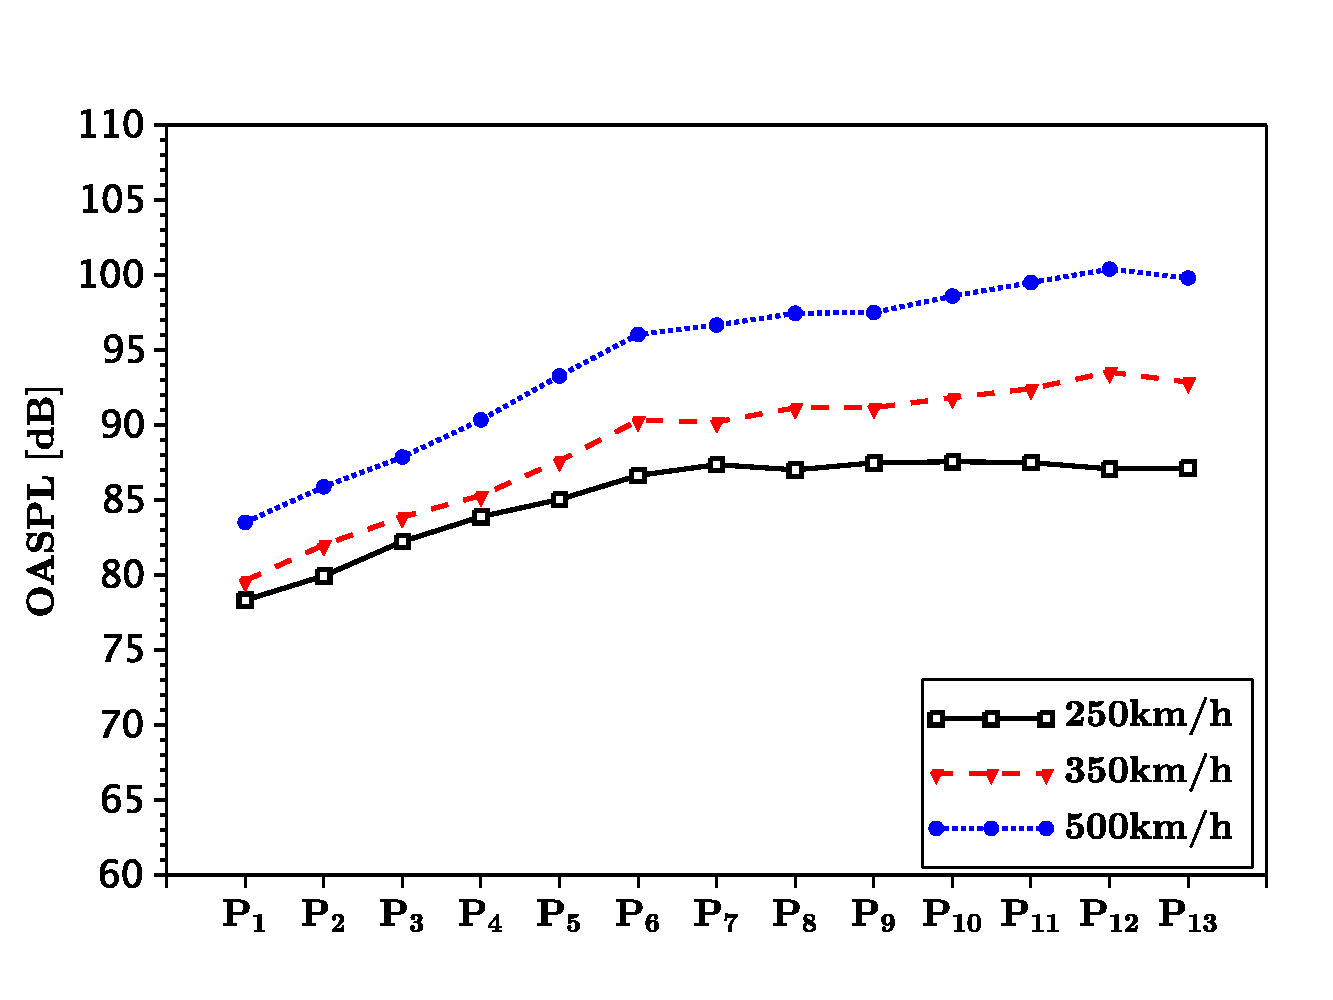
\includegraphics[width=0.55\textwidth]{Figures/oaspl_a.pdf}
  \neufigcaption{fig:ch0-cover}{外部图片插入样例}{Example of Including an External Image}
\end{figure}

\neufigref{fig:ch0-cover} 展示了通过 \verb|\includegraphics| 插入图片文件的方式。
正式论文中建议将图片统一放入 \texttt{Figures} 目录，并使用相对路径引用。

\subsection{PDF 或位图图片}
\begin{figure}[!htbp]
  \centering
  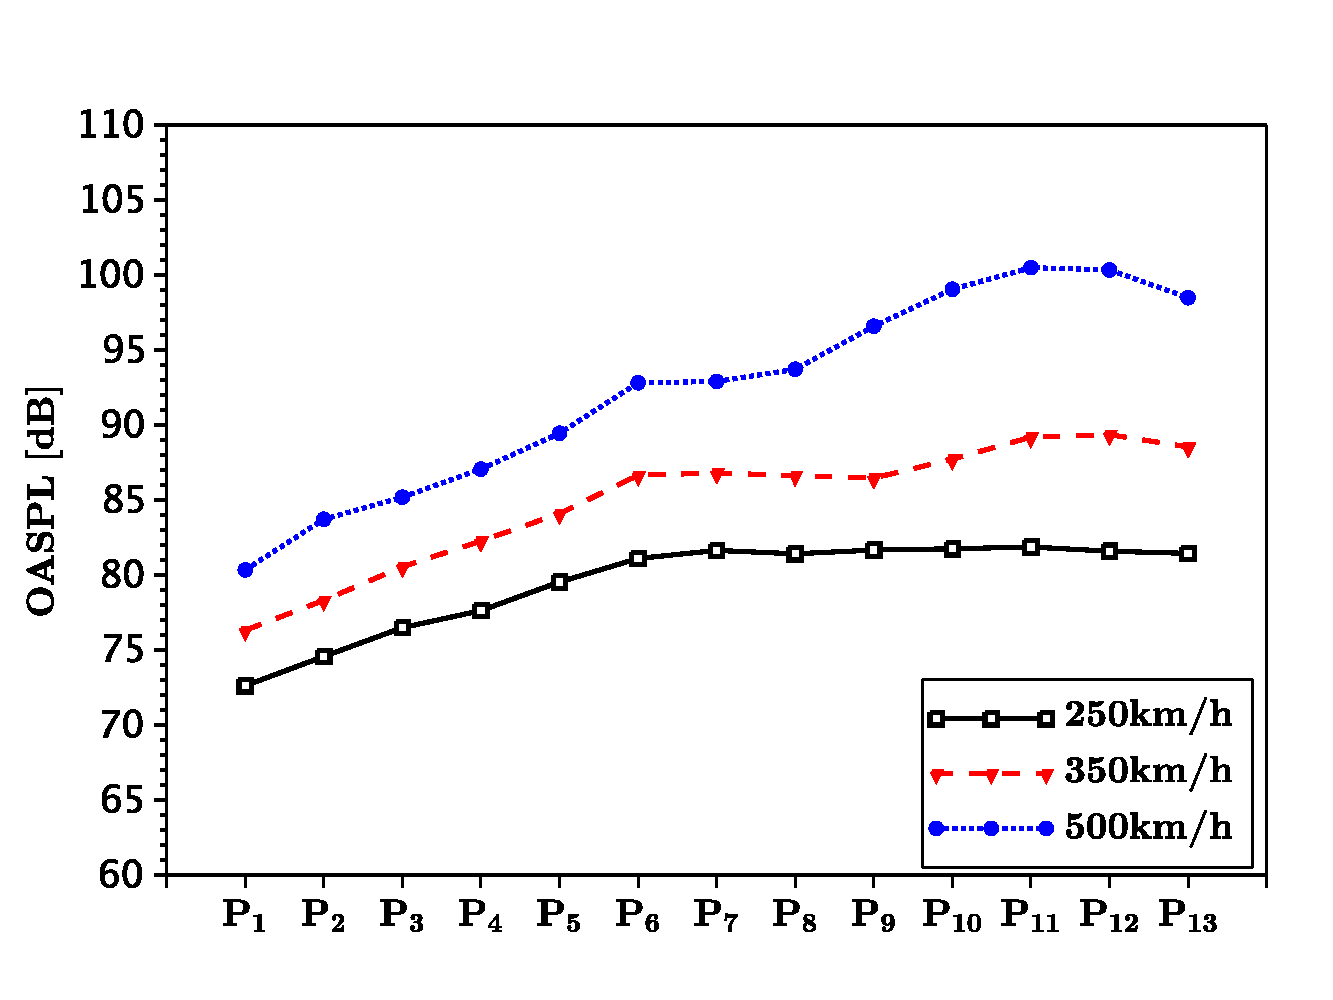
\includegraphics[width=0.55\textwidth]{Figures/oaspl_b.pdf}
  \neufigcaption{fig:ch0-pdf}{PDF 图片插入样例}{Example of Including a PDF Figure}
\end{figure}

PDF、PNG、JPG 等常见图片格式均可通过 \verb|\includegraphics| 插入。
若图片由绘图软件或数据分析程序导出，建议优先使用 PDF 格式以保持较清晰的显示效果。

\subsection{并列图片}
\begin{figure}[!htbp]
  \centering
  \begin{minipage}[t]{0.49\linewidth}
    \centering
    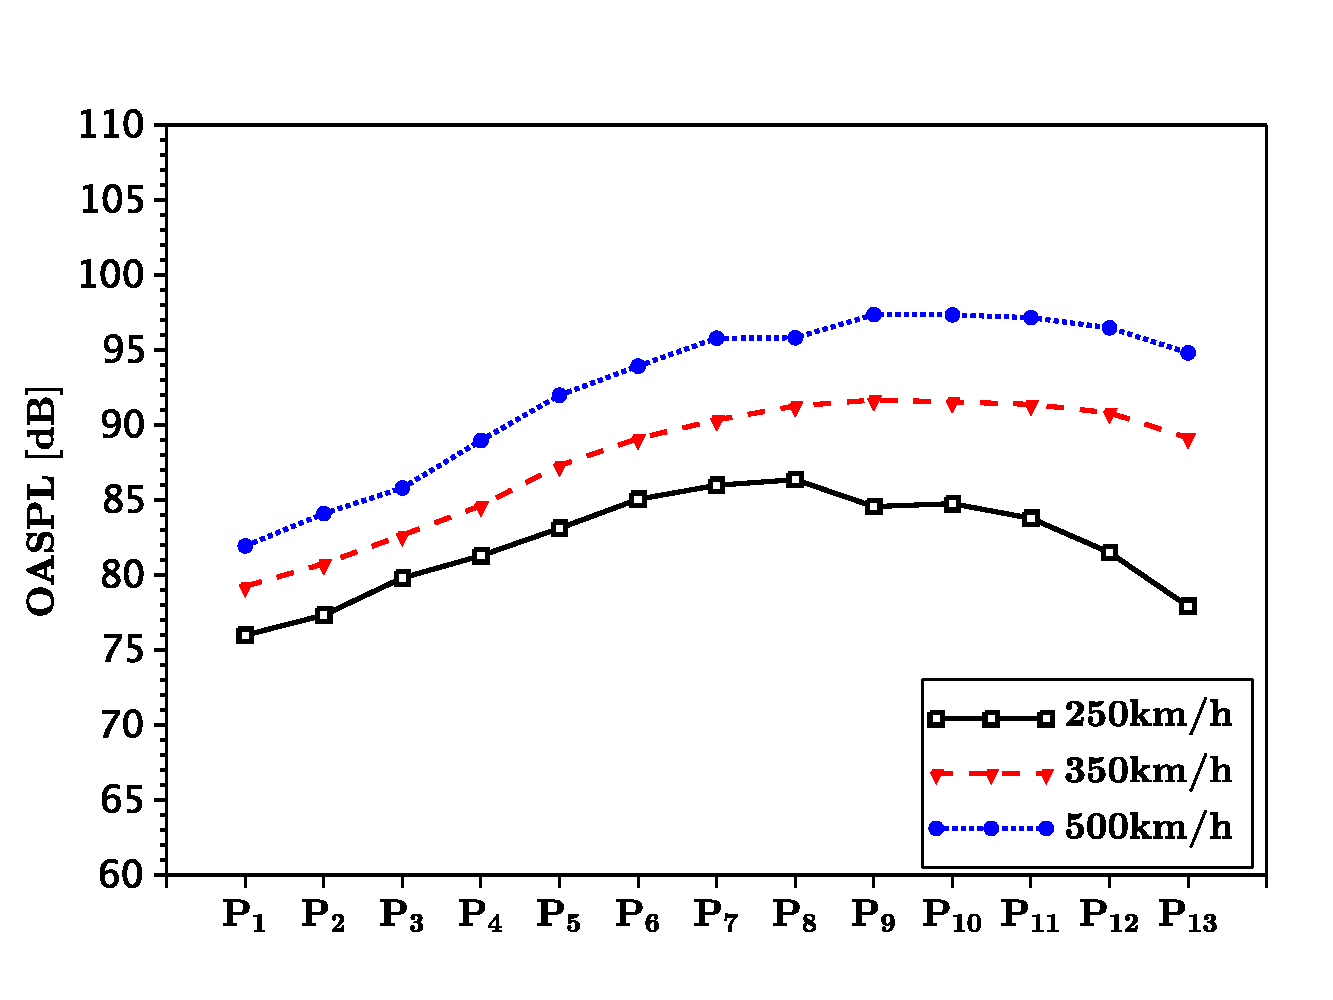
\includegraphics[width=\linewidth]{Figures/oaspl_c.pdf}
  \end{minipage}
  \hfill
  \begin{minipage}[t]{0.49\linewidth}
    \centering
    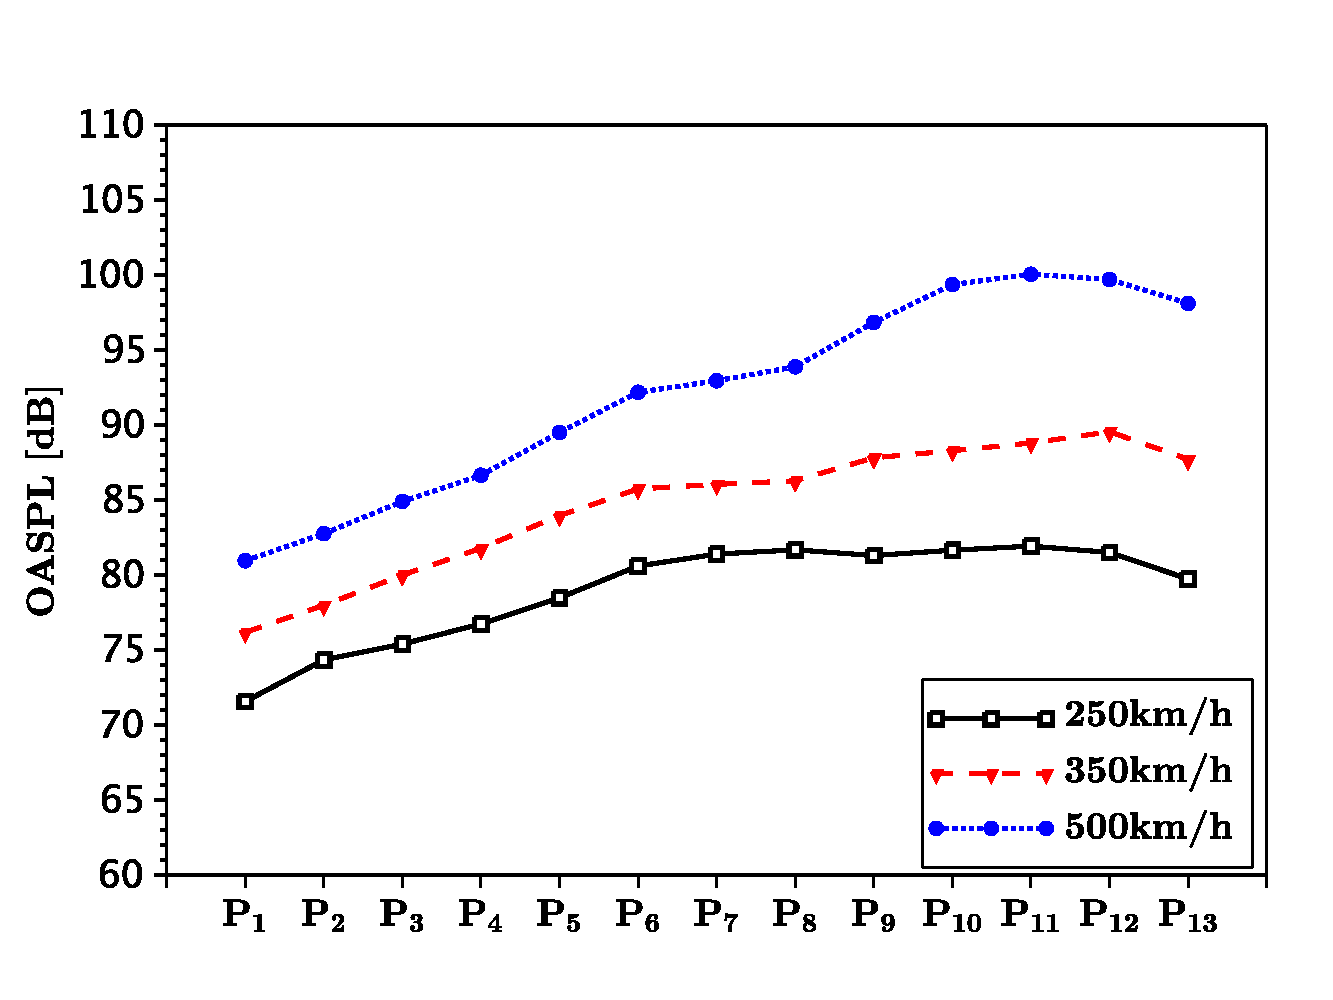
\includegraphics[width=\linewidth]{Figures/oaspl_d.pdf}
  \end{minipage}
  \neufigcaption{fig:ch0-side-by-side}{普通并列图形排版样例}{Example of Side-by-Side Figures}
\end{figure}

\neufigref{fig:ch0-side-by-side} 使用 \texttt{minipage} 完成普通并列排版。
当两幅图共享一个总标题且不需要分别引用时，可使用这种方式。

\subsection{并列子图}
\begin{figure}[!htbp]
  \centering
  \begin{neusubfigure}{0.49\linewidth}
    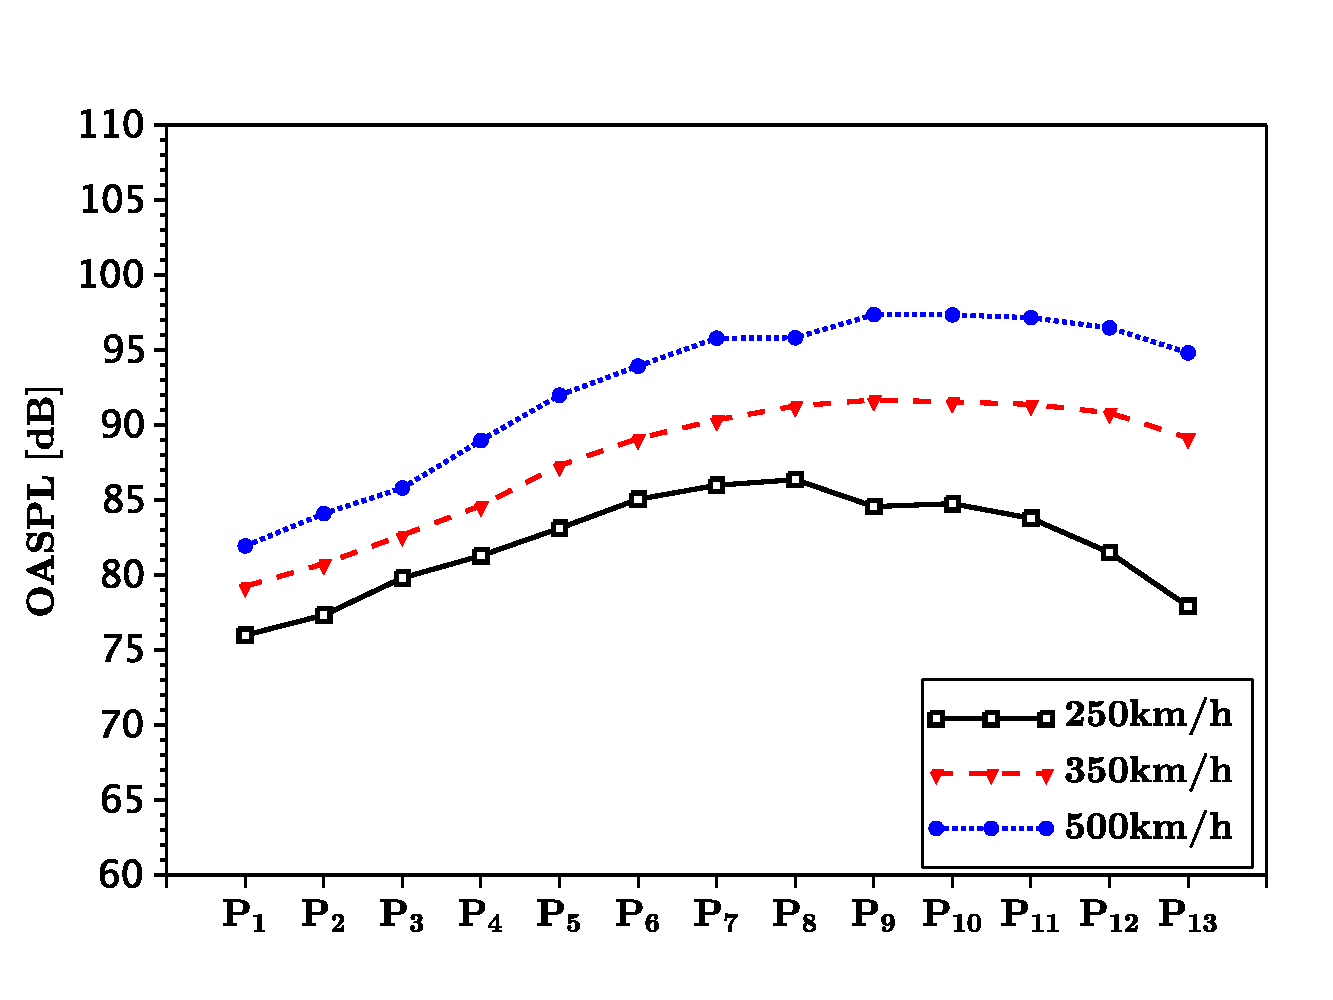
\includegraphics[width=\linewidth]{Figures/oaspl_c.pdf}
    \neusubfigcaption{fig:ch0-side-by-side-a}{工况一}
  \end{neusubfigure}
  \hfill
  \begin{neusubfigure}{0.49\linewidth}
    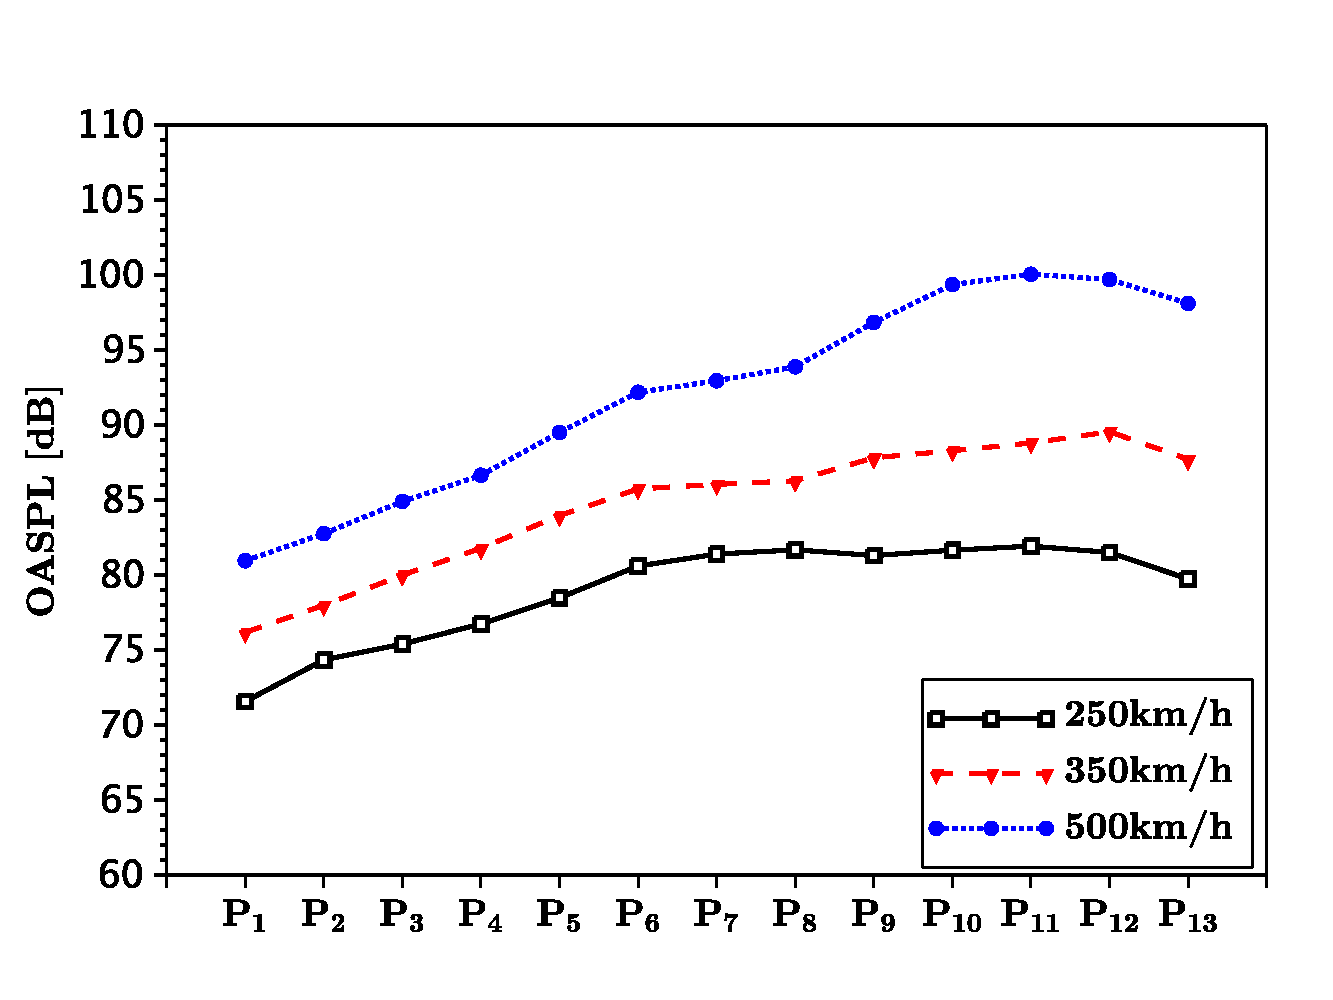
\includegraphics[width=\linewidth]{Figures/oaspl_d.pdf}
    \neusubfigcaption{fig:ch0-side-by-side-b}{工况二}
  \end{neusubfigure}
  \neufigcaption{fig:ch0-subfigures}{并列子图排版样例}{Example of Side-by-Side Subfigures}
\end{figure}

\neufigref{fig:ch0-subfigures} 使用 \texttt{neusubfigure} 完成并列子图排版。
其中 \neusubfigref{fig:ch0-side-by-side-a} 和 \neusubfigref{fig:ch0-side-by-side-b} 可分别引用到子图。
当两幅图共享一个总标题且需要分别引用时，可使用这种方式；如果每幅图需要完全独立的图号，建议拆成两个独立的 \texttt{figure} 环境。

\subsection{二乘二子图}
\begin{figure}[!htbp]
  \centering
  \begin{neusubfigure}{0.49\linewidth}
    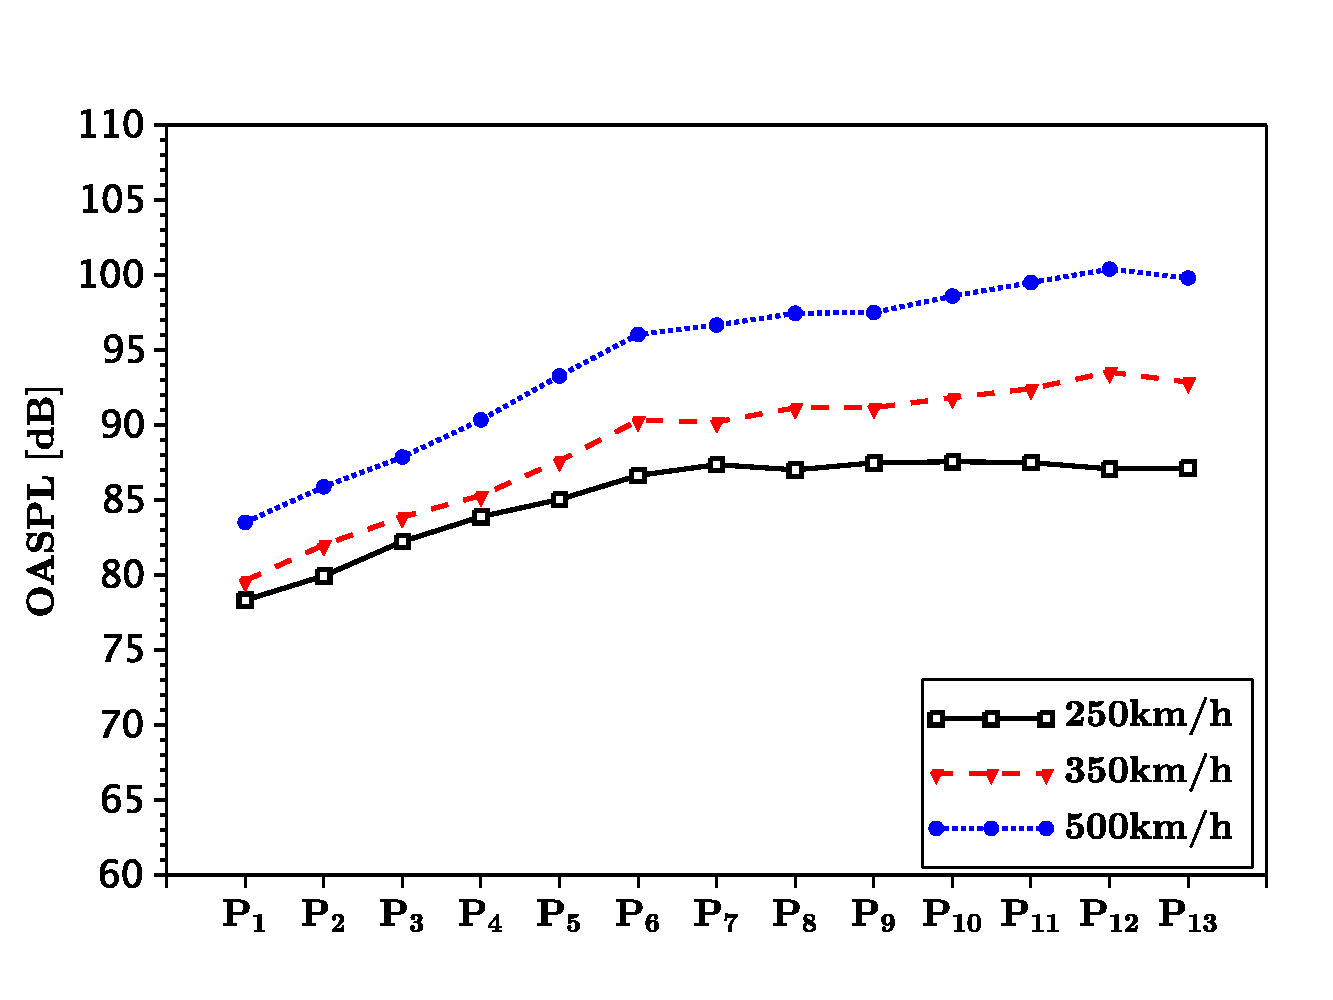
\includegraphics[width=\linewidth]{Figures/oaspl_a.pdf}
    \neusubfigcaption{fig:ch0-four-subfig-a}{工况一}
  \end{neusubfigure}
  \hfill
  \begin{neusubfigure}{0.49\linewidth}
    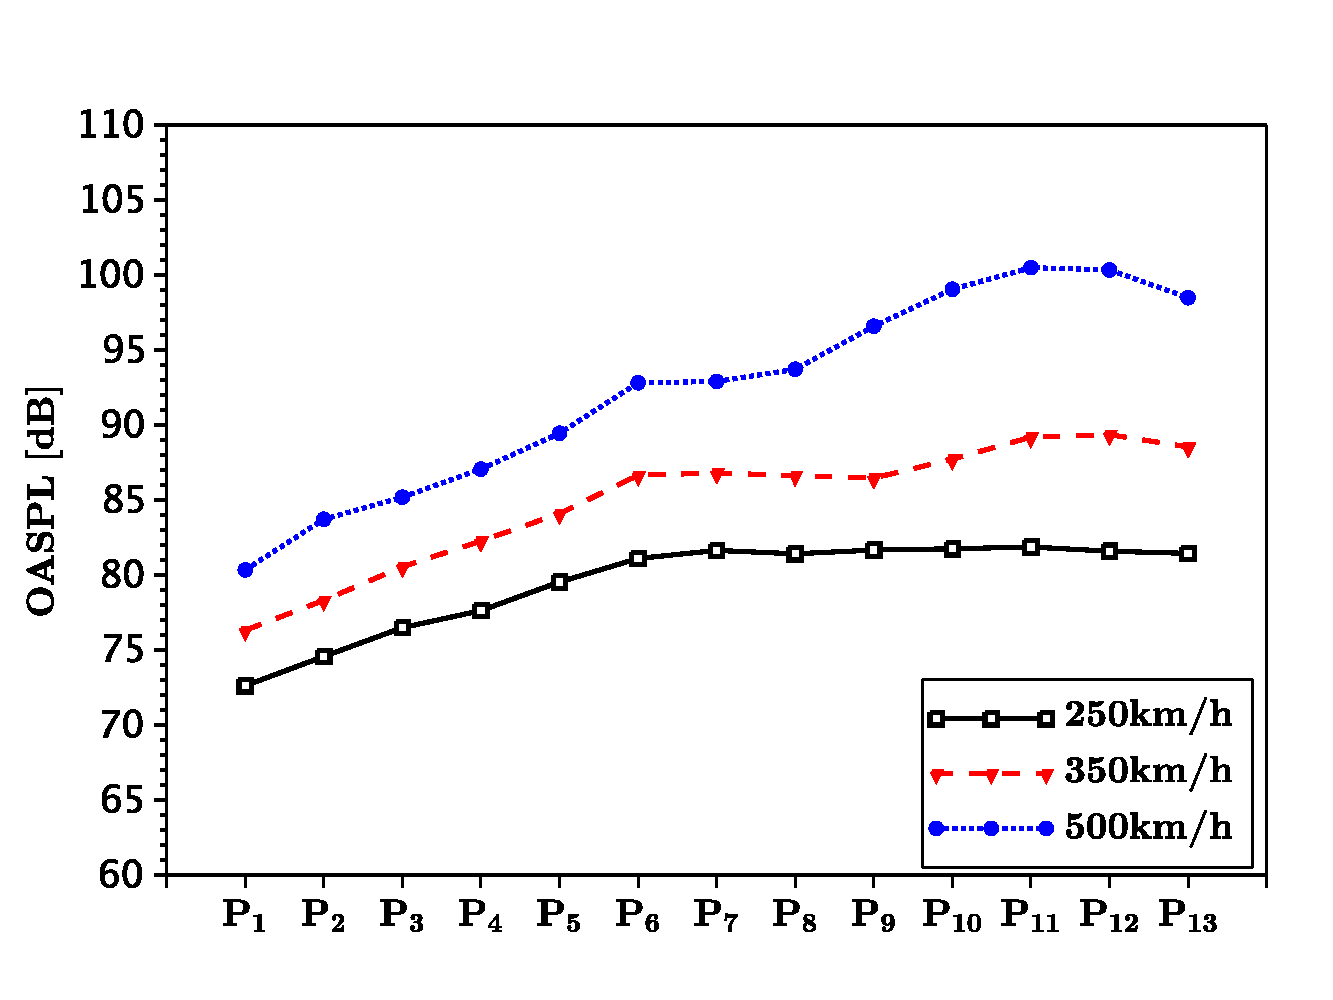
\includegraphics[width=\linewidth]{Figures/oaspl_b.pdf}
    \neusubfigcaption{fig:ch0-four-subfig-b}{工况二}
  \end{neusubfigure}
  \par\vspace{2bp}

  \begin{neusubfigure}{0.49\linewidth}
    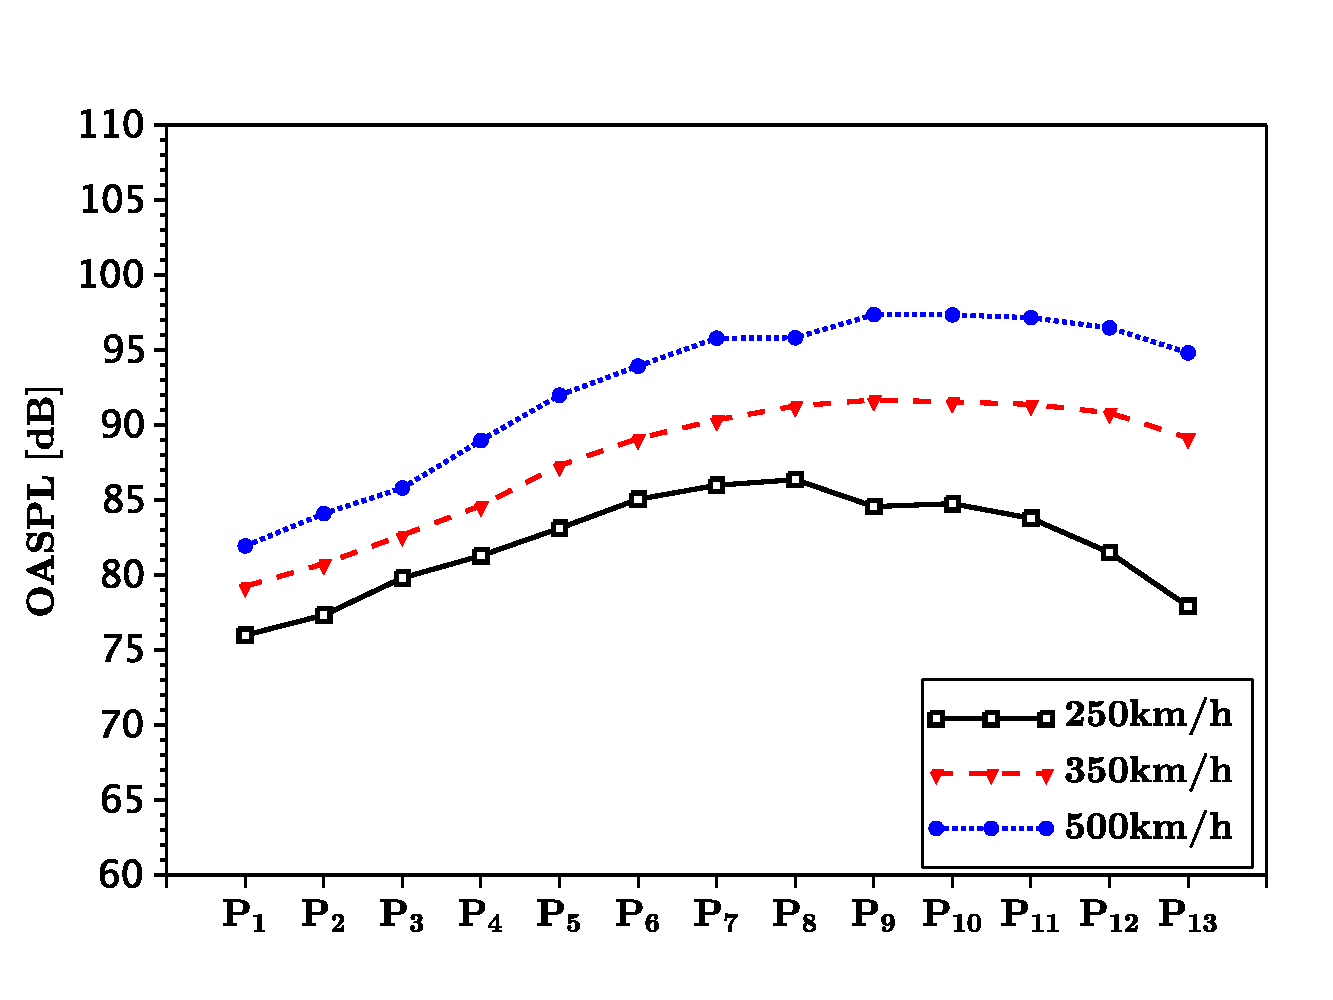
\includegraphics[width=\linewidth]{Figures/oaspl_c.pdf}
    \neusubfigcaption{fig:ch0-four-subfig-c}{工况三}
  \end{neusubfigure}
  \hfill
  \begin{neusubfigure}{0.49\linewidth}
    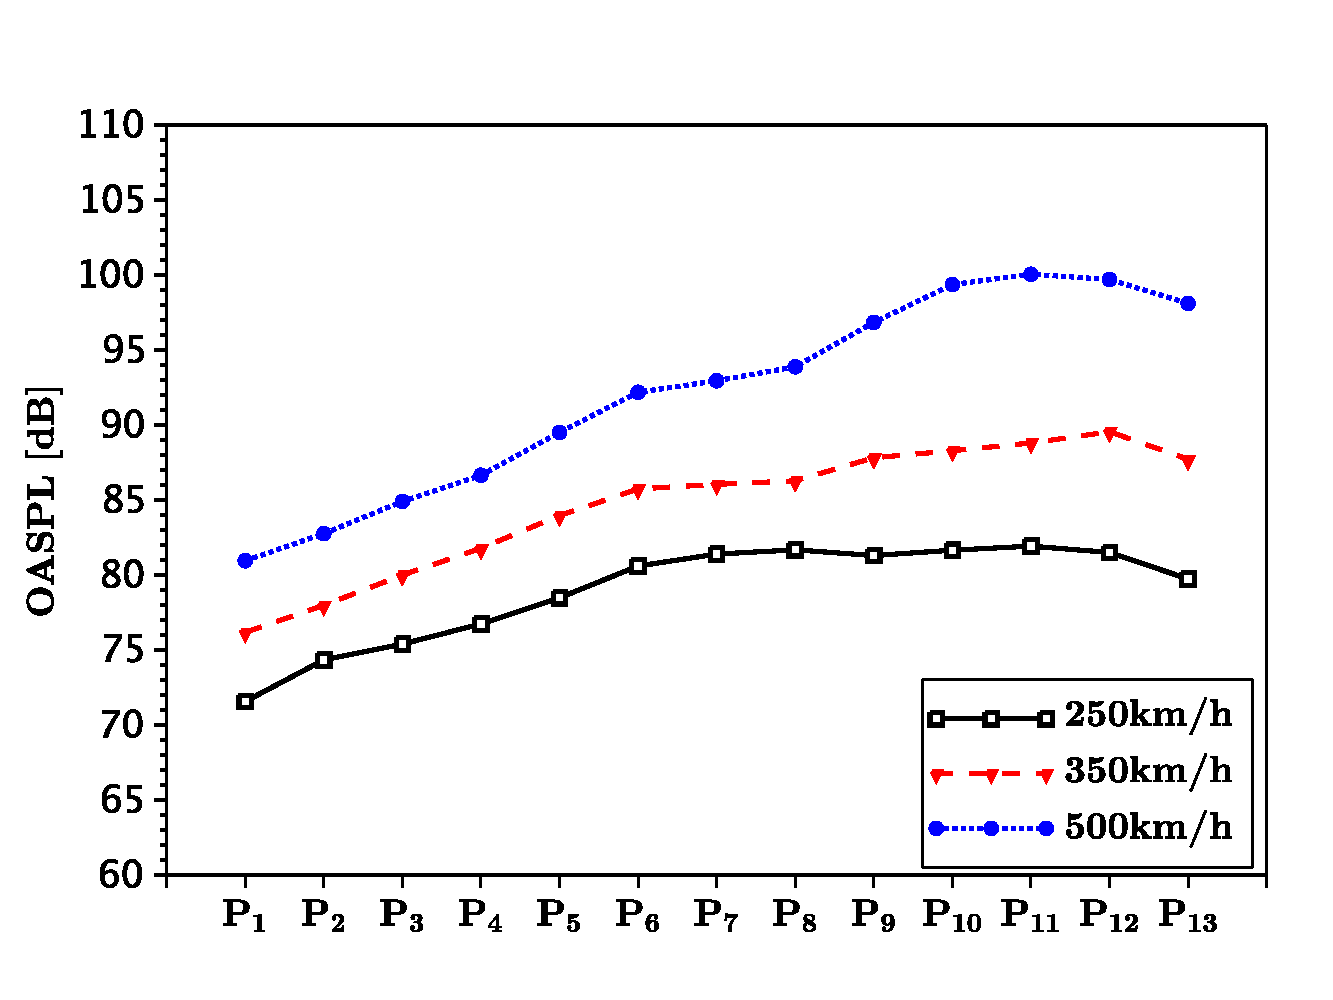
\includegraphics[width=\linewidth]{Figures/oaspl_d.pdf}
    \neusubfigcaption{fig:ch0-four-subfig-d}{工况四}
  \end{neusubfigure}
  \neufigcaption{fig:ch0-four-subfigures}{二乘二子图排版样例}{Example of Two-by-Two Subfigures}
\end{figure}

\neufigref{fig:ch0-four-subfigures} 展示了四幅子图的二乘二排布。
例如 \neusubfigref{fig:ch0-four-subfig-a} 至 \neusubfigref{fig:ch0-four-subfig-d} 可分别引用到四个子图。
排版时建议注意以下几点：
\begin{itemize}
  \item 子图宽度通常可取 \verb|0.48\linewidth| 至 \verb|0.49\linewidth|。
  \item 每行两个子图之间使用 \verb|\hfill| 自动拉开横向间距。
  \item 两行之间可用少量 \verb|\par\vspace| 控制垂直间距。
\end{itemize}

\section{表格排版}

本模板提供 \verb|\neutabcaption{label}{中文题名}{English title}| 用于生成中英文表题。
表题应置于表格上方，正文中使用 \verb|\neutabref{label}| 引用。
表格同样建议使用 \verb|[!htbp]|。如果表格过高导致页底空白，优先考虑缩小字号、调整列宽、拆分表格或使用跨页表格，而不是强制分页。

\subsection{三线表}

\begin{table}[!htbp]
  \centering
  \neutabcaption{tab:ch0-booktabs}{三线表样例}{Example of a Three-Line Table}
  \begin{tabular}{lccc}
    \toprule
    方法       & 准确率（\%）       & 召回率（\%）       & F1 值           \\
    \midrule
    Baseline & 85.2          & 84.1          & 0.846          \\
    Method A & 89.7          & 88.9          & 0.893          \\
    Proposed & \textbf{92.1} & \textbf{91.5} & \textbf{0.918} \\
    \bottomrule
  \end{tabular}
\end{table}

\neutabref{tab:ch0-booktabs} 展示了推荐的三线表格式。
论文中应尽量避免过多竖线，以保持表格简洁。

\subsection{复杂表格}
\begin{table}[!htbp]
  \centering
  \neutabcaption{tab:ch0-complex}{合并单元格与自动换行表格样例}{Example of Merged Cells and Auto-Wrapping Columns}
  \begin{tabularx}{\textwidth}{llXc}
    \toprule
    类别                  & 指标  & 说明                               & 是否必需 \\
    \midrule
    \multirow{2}{*}{图形} & 分辨率 & 位图图片应保证在最终 PDF 中清晰可辨。            & 是    \\
                        & 题名  & 图题使用中英文双语标题，并位于图片下方。             & 是    \\
    \midrule
    \multirow{2}{*}{表格} & 宽度  & 宽表格可使用 \texttt{tabularx} 自动分配列宽。 & 否    \\
                        & 表注  & 表内说明应简明，必要时可在正文中解释。              & 否    \\
    \bottomrule
  \end{tabularx}
\end{table}

\neutabref{tab:ch0-complex} 同时展示了 \verb|\multirow|、\verb|\makecell| 可配合使用的复杂表格场景。
若单元格内容较长，优先使用 \texttt{tabularx} 或 \texttt{p\{...\}} 列类型控制宽度。

\section{公式排版}

公式应使用标准数学环境，并通过 \verb|\label| 设置标签。
引用公式时建议使用模板提供的 \verb|\neueqref{label}|。

\subsection{单行公式}
以分类任务中的交叉熵损失为例，可写为
\begin{equation}
  \mathcal{L}(\theta)
  = - \frac{1}{N}\sum_{i=1}^{N}\sum_{k=1}^{K} y_{ik}\log p_{ik}
  \label{eq:ch0-loss}
\end{equation}

如 \neueqref{eq:ch0-loss} 所示，带编号公式适合放置正文中需要引用的重要定义。

\subsection{多行公式}
循环模型中的状态更新和输出计算可写为
\begin{align}
  h_t       & = \sigma(W_x x_t + W_h h_{t-1} + b), \label{eq:ch0-state} \\
  \hat{y}_t & = \operatorname{softmax}(W_o h_t). \label{eq:ch0-output}
\end{align}

\neueqref{eq:ch0-state} 和 \neueqref{eq:ch0-output} 展示了多行公式的编号方式。
如果多行推导只需要一个编号，可使用 \texttt{aligned} 放在 \texttt{equation} 环境内部。

\subsection{分段函数与矩阵}
分段函数和矩阵经常同时出现在数学定义中，例如
\begin{equation}
  g(x)=
  \begin{cases}
    0, & x < 0,       \\
    x, & 0 \le x < 1, \\
    1, & x \ge 1,
  \end{cases}
  \qquad
  A =
  \begin{bmatrix}
    1 & 0 & 0 \\
    0 & 1 & 0 \\
    0 & 0 & 1
  \end{bmatrix}.
  \label{eq:ch0-piecewise}
\end{equation}

\neueqref{eq:ch0-piecewise} 展示了分段函数和矩阵的常见写法。

\section{算法伪代码}

计算机类论文常需要给出算法步骤。本文档在 \texttt{main.tex} 中加载了 \texttt{algorithm} 和 \texttt{algorithmic} 宏包，可以直接使用如下环境。

\begin{algorithm}[!htbp]
  \caption{样例训练流程}
  \label{alg:ch0-training}
  \begin{algorithmic}[1]
    \REQUIRE Training set $\mathcal{D}$, learning rate $\eta$, maximum epoch $T$
    \ENSURE Model parameters $\theta$
    \STATE Initialize parameters $\theta$
    \FOR{$t = 1$ to $T$}
    \STATE Sample a mini-batch $\mathcal{B}$ from $\mathcal{D}$
    \STATE Compute loss $\mathcal{L}(\theta)$ by \neueqref{eq:ch0-loss}
    \STATE Update $\theta \leftarrow \theta - \eta \nabla_{\theta}\mathcal{L}(\theta)$
    \ENDFOR
    \RETURN $\theta$
  \end{algorithmic}
\end{algorithm}

算法~\ref{alg:ch0-training} 展示了带行号的伪代码。
若需要中文关键字，可在导言区重定义相应命令。

\section{引用、链接与交叉引用}

参考文献引用可使用两种模板命令：
\begin{itemize}
  \item 上标引用使用 \verb|\upcite{key}|，适合放在句末，例如已有研究讨论了神经网络轻量化问题\upcite{guo_2023_research}。
  \item 正文引用使用 \verb|\inlinecite{key}|，适合作为句子成分，例如文献 \inlinecite{thakkar_2018_performance} 给出了系统性能评测案例。
\end{itemize}
多篇文献可写在同一条引用命令中，例如区块链平台相关研究\upcite{zheng_2019_nutbaas,thakkar_2018_performance}。

交叉引用建议统一使用模板命令：
\begin{itemize}
  \item 图引用：\verb|\neufigref{fig:ch0-pdf}|，效果为 \neufigref{fig:ch0-pdf}。
  \item 子图引用：\verb|\neusubfigref{fig:ch0-four-subfig-a}|，效果为 \neusubfigref{fig:ch0-four-subfig-a}。
  \item 表引用：\verb|\neutabref{tab:ch0-complex}|，效果为 \neutabref{tab:ch0-complex}。
  \item 公式引用：\verb|\neueqref{eq:ch0-loss}|，效果为 \neueqref{eq:ch0-loss}。
  \item 算法引用：当前模板未单独封装算法引用命令，可写作“算法~\ref{alg:ch0-training}”。
\end{itemize}
模板提供的公开命令和环境可参考 \texttt{README.md} 中的“模板命令说明”一节。
|，并从第~\ref{chap:introduction}~章开始组织正式内容。

\section{章节层级与正文段落}

论文正文通常从一级标题开始组织内容，一级标题使用 \verb|\chapter|，二级标题使用 \verb|\section|，三级标题使用 \verb|\subsection|。
本模板会自动设置章标题、节标题、页眉、页码和目录格式，作者只需要关注正文内容。
正文段落首行缩进、行距和中英文字体均由模板统一控制，一般不需要在正文中手动设置字号、字体或段间距。

中文正文可以直接书写；英文术语建议在首次出现时给出全称，例如自然语言处理（Natural Language Processing, NLP）。
行内公式可以写作 $E=mc^2$，行内代码或命令可以使用 \verb|\verb|，例如 \verb|%!TEX root = ./main.tex
\chapter{论文格式样例与模板验证}

本章作为模板的集中样例章，用于快速检查正文中常见排版元素的显示效果。
样例覆盖章节层级、正文段落、列表、脚注、图、表、公式、算法、交叉引用和参考文献引用等内容。
编写正式论文时，可以保留本章作为排版对照；定稿前可在 \texttt{main.tex} 中删除或注释 \verb|\input{chapter0-guide}|，并从第~\ref{chap:introduction}~章开始组织正式内容。

\section{章节层级与正文段落}

论文正文通常从一级标题开始组织内容，一级标题使用 \verb|\chapter|，二级标题使用 \verb|\section|，三级标题使用 \verb|\subsection|。
本模板会自动设置章标题、节标题、页眉、页码和目录格式，作者只需要关注正文内容。
正文段落首行缩进、行距和中英文字体均由模板统一控制，一般不需要在正文中手动设置字号、字体或段间距。

中文正文可以直接书写；英文术语建议在首次出现时给出全称，例如自然语言处理（Natural Language Processing, NLP）。
行内公式可以写作 $E=mc^2$，行内代码或命令可以使用 \verb|\verb|，例如 \verb|\input{chapter0-guide}|。
脚注示例如此处所示\footnote{脚注用于补充说明，不宜放置过长的正文内容。}。
若某页因图表浮动或分页规则没有排满，脚注可能跟随正文排版区而显得略高，这是正常的 LaTeX 页面构建结果。

\subsection{字体、字号与强调}

模板预定义了常用中文字体命令。正式论文中通常不需要手动切换字体；只有在展示样式、术语强调或特殊说明时才建议使用。
当前模板已经为默认宋体和 \verb|\song| 字族配置伪粗体，因此 \verb|\textbf| 或 \verb|\bfseries| 可以用于中文局部强调。
需要注意的是，中文加粗应克制使用；标题层级、术语定义或表格重点值可以适当加粗，大段正文不建议整体加粗。
如果需要更明显的标题式强调，可使用黑体或调整标题层级；如果只是普通正文重点，优先使用 \verb|\textbf|。

\begin{table}[!htbp]
  \centering
  \neutabcaption{tab:ch0-fonts}{字体与强调样例}{Examples of Fonts and Emphasis}
  \begin{tabular}{lll}
    \toprule
    命令             & 显示效果                         & 使用建议       \\
    \midrule
    \verb|\song|   & {\song 宋体文字示例}               & 正文默认字体     \\
    \verb|\textbf| & \textbf{加粗文字示例}              & 局部强调、表格重点值 \\
    \verb|\hei|    & {\hei 黑体文字示例}                & 标题或较强强调场景  \\
    \verb|\kai|    & {\kai 楷体文字示例}                & 摘要、题签或引用语  \\
    \verb|\fs|     & {\fs 仿宋文字示例}                 & 特殊文书类内容    \\
    \verb|\textit| & \textit{Italic text example} & 英文斜体或变量说明  \\
    \bottomrule
  \end{tabular}
\end{table}

\subsection{列表环境}

无序列表适合列出并列事项：
\begin{itemize}
  \item 图题位于图下方，表题位于表上方。
  \item 图表应使用中英文双语标题。
  \item 公式、图、表、算法均应使用标签进行交叉引用。
\end{itemize}

有序列表适合描述步骤：
\begin{enumerate}
  \item 在 \texttt{main.tex} 中填写论文元信息。
  \item 在各章文件中撰写正文内容。
  \item 使用 \texttt{latexmk -xelatex main.tex} 完成编译。
\end{enumerate}

\section{图形排版}

本模板提供 \verb|\neufigcaption{label}{中文题名}{English title}| 用于生成中英文图题。
图题应置于图形下方，正文中使用 \verb|\neufigref{label}| 引用。
图形建议使用 \verb|[!htbp]| 浮动参数，让 LaTeX 在当前位置、页顶、页底或浮动页中选择较合适的位置；除非必须固定位置，否则不建议使用 \verb|[H]|。

\subsection{外部图片}
\begin{figure}[!htbp]
  \centering
  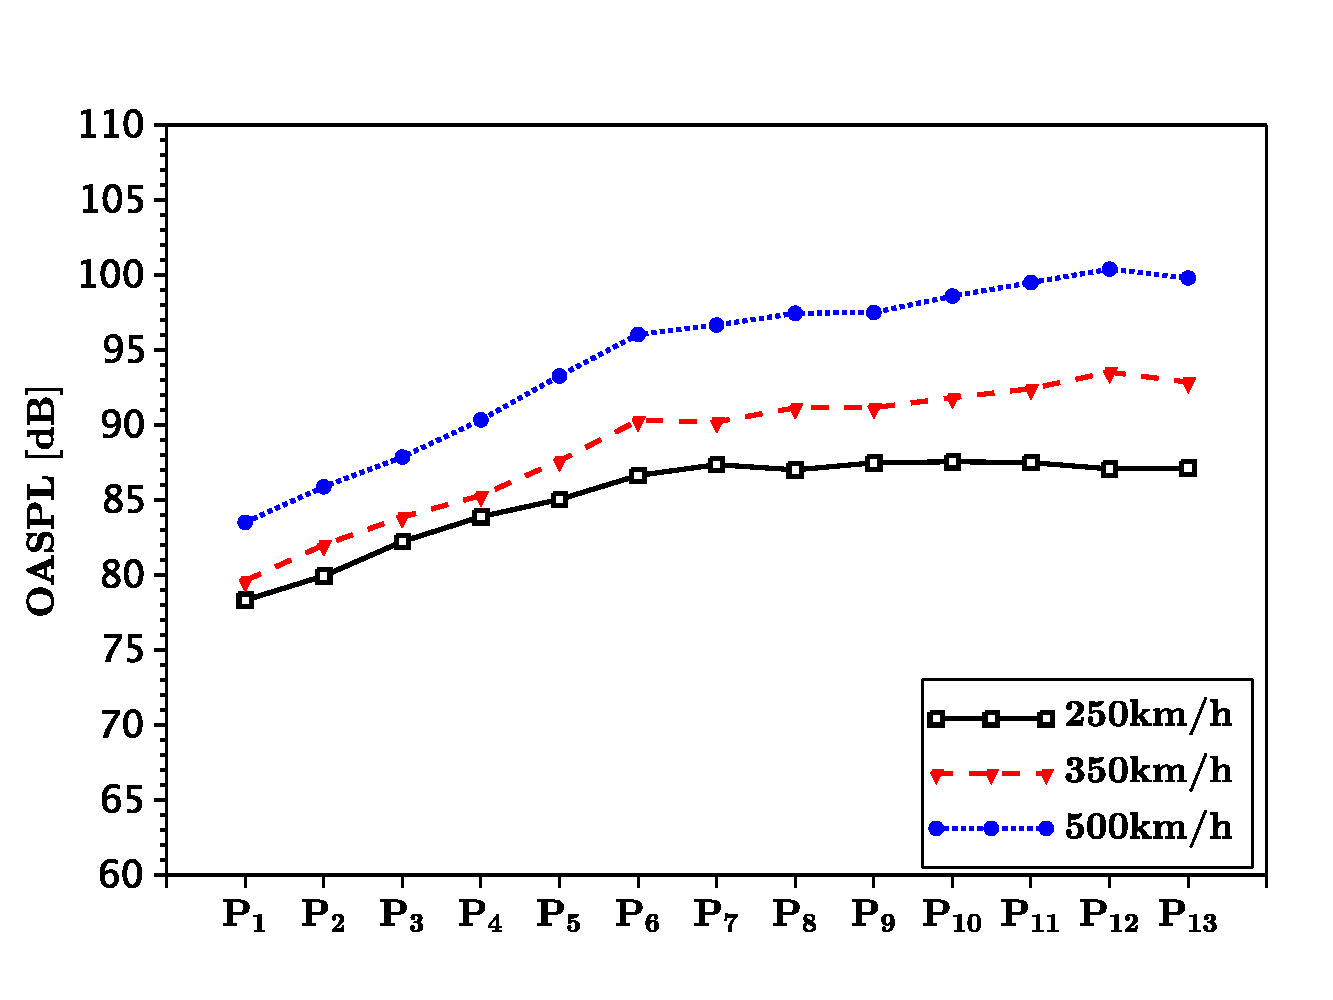
\includegraphics[width=0.55\textwidth]{Figures/oaspl_a.pdf}
  \neufigcaption{fig:ch0-cover}{外部图片插入样例}{Example of Including an External Image}
\end{figure}

\neufigref{fig:ch0-cover} 展示了通过 \verb|\includegraphics| 插入图片文件的方式。
正式论文中建议将图片统一放入 \texttt{Figures} 目录，并使用相对路径引用。

\subsection{PDF 或位图图片}
\begin{figure}[!htbp]
  \centering
  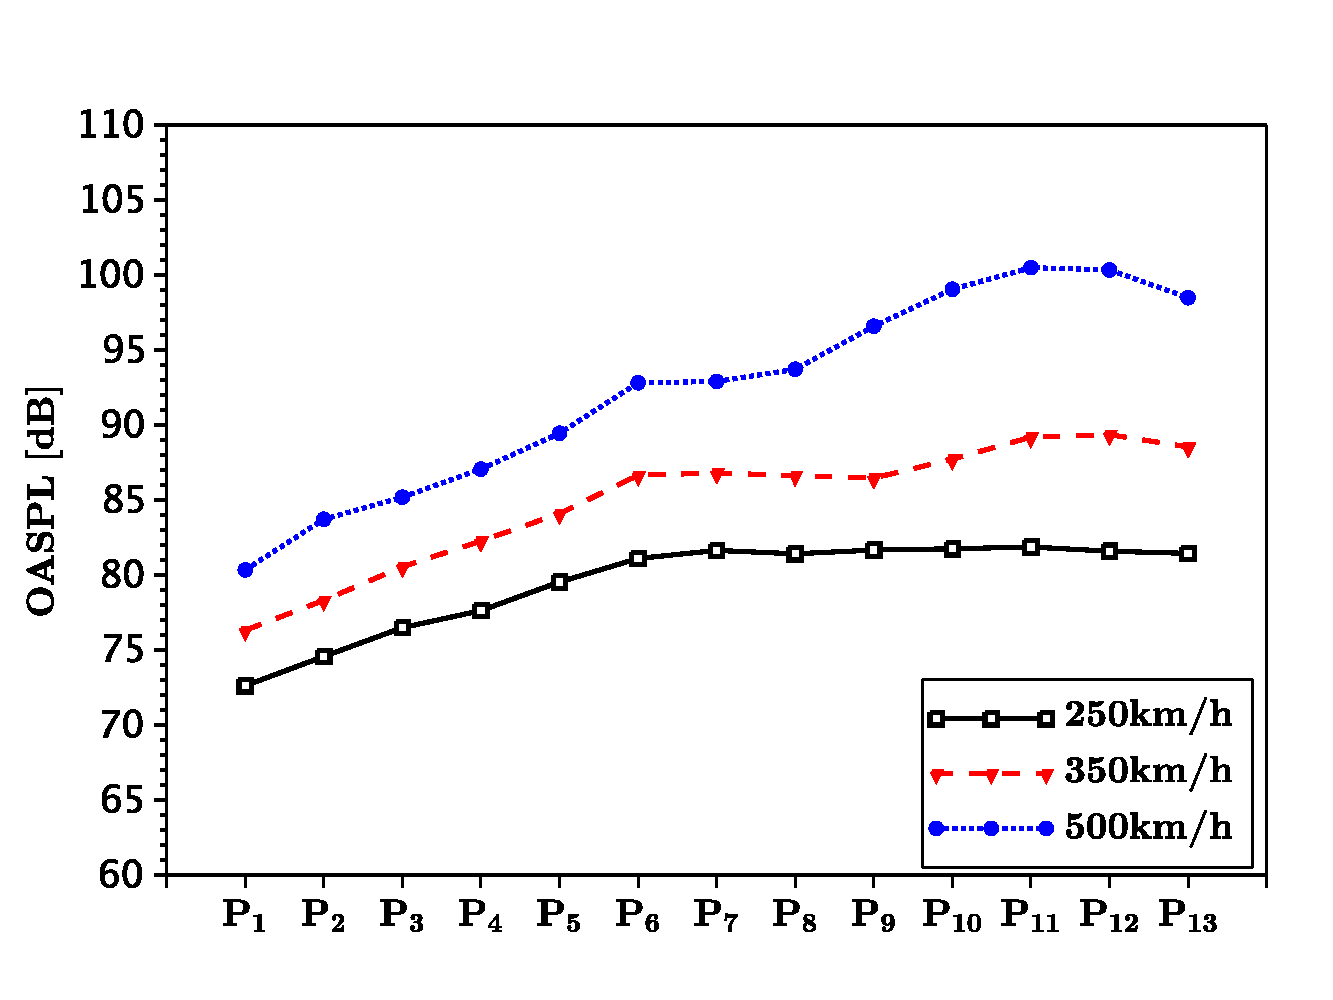
\includegraphics[width=0.55\textwidth]{Figures/oaspl_b.pdf}
  \neufigcaption{fig:ch0-pdf}{PDF 图片插入样例}{Example of Including a PDF Figure}
\end{figure}

PDF、PNG、JPG 等常见图片格式均可通过 \verb|\includegraphics| 插入。
若图片由绘图软件或数据分析程序导出，建议优先使用 PDF 格式以保持较清晰的显示效果。

\subsection{并列图片}
\begin{figure}[!htbp]
  \centering
  \begin{minipage}[t]{0.49\linewidth}
    \centering
    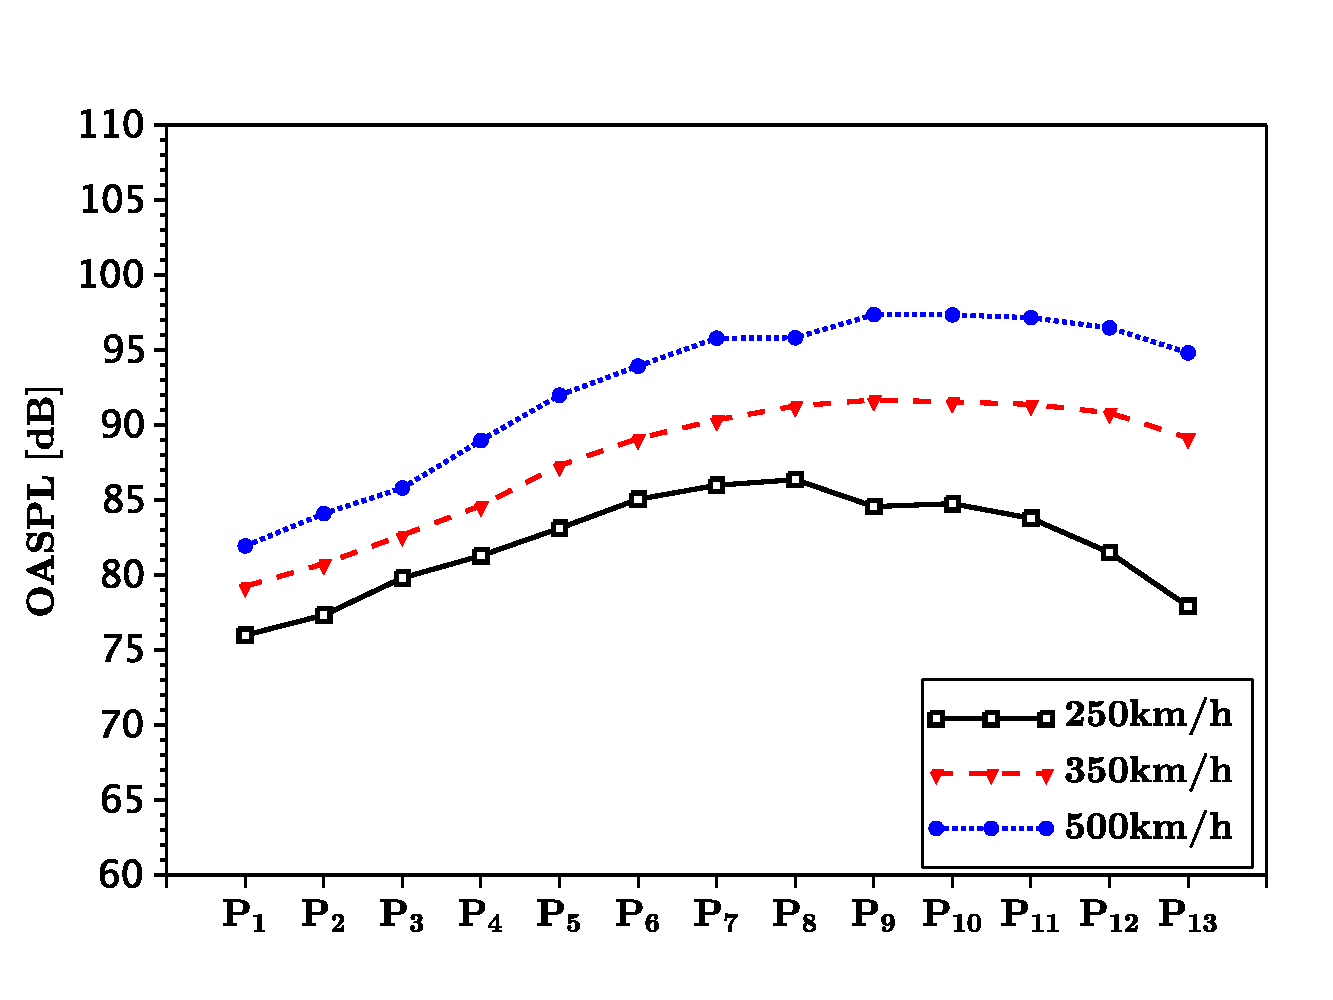
\includegraphics[width=\linewidth]{Figures/oaspl_c.pdf}
  \end{minipage}
  \hfill
  \begin{minipage}[t]{0.49\linewidth}
    \centering
    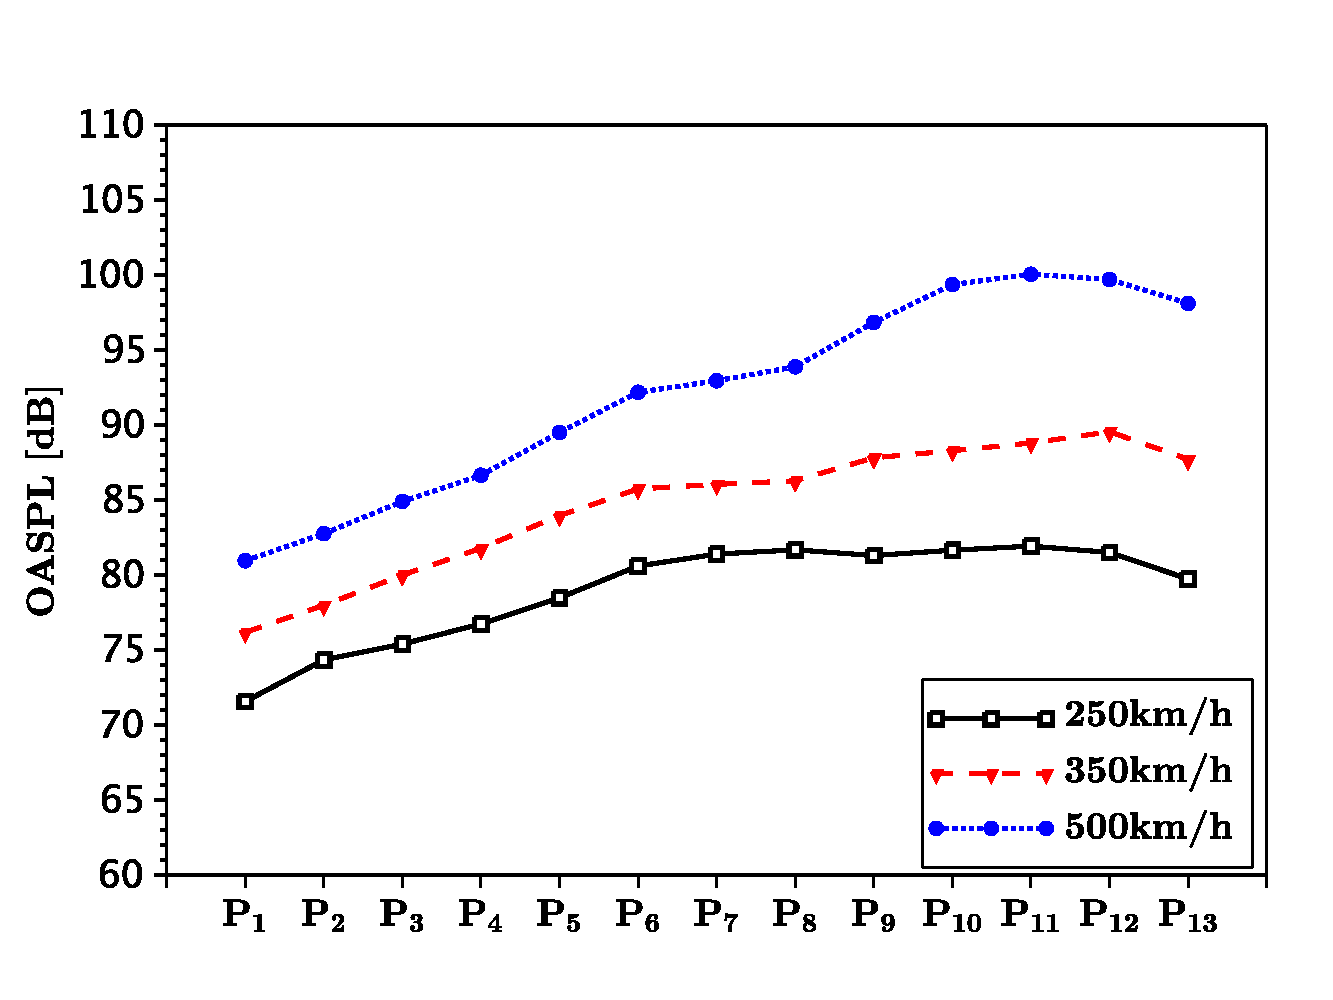
\includegraphics[width=\linewidth]{Figures/oaspl_d.pdf}
  \end{minipage}
  \neufigcaption{fig:ch0-side-by-side}{普通并列图形排版样例}{Example of Side-by-Side Figures}
\end{figure}

\neufigref{fig:ch0-side-by-side} 使用 \texttt{minipage} 完成普通并列排版。
当两幅图共享一个总标题且不需要分别引用时，可使用这种方式。

\subsection{并列子图}
\begin{figure}[!htbp]
  \centering
  \begin{neusubfigure}{0.49\linewidth}
    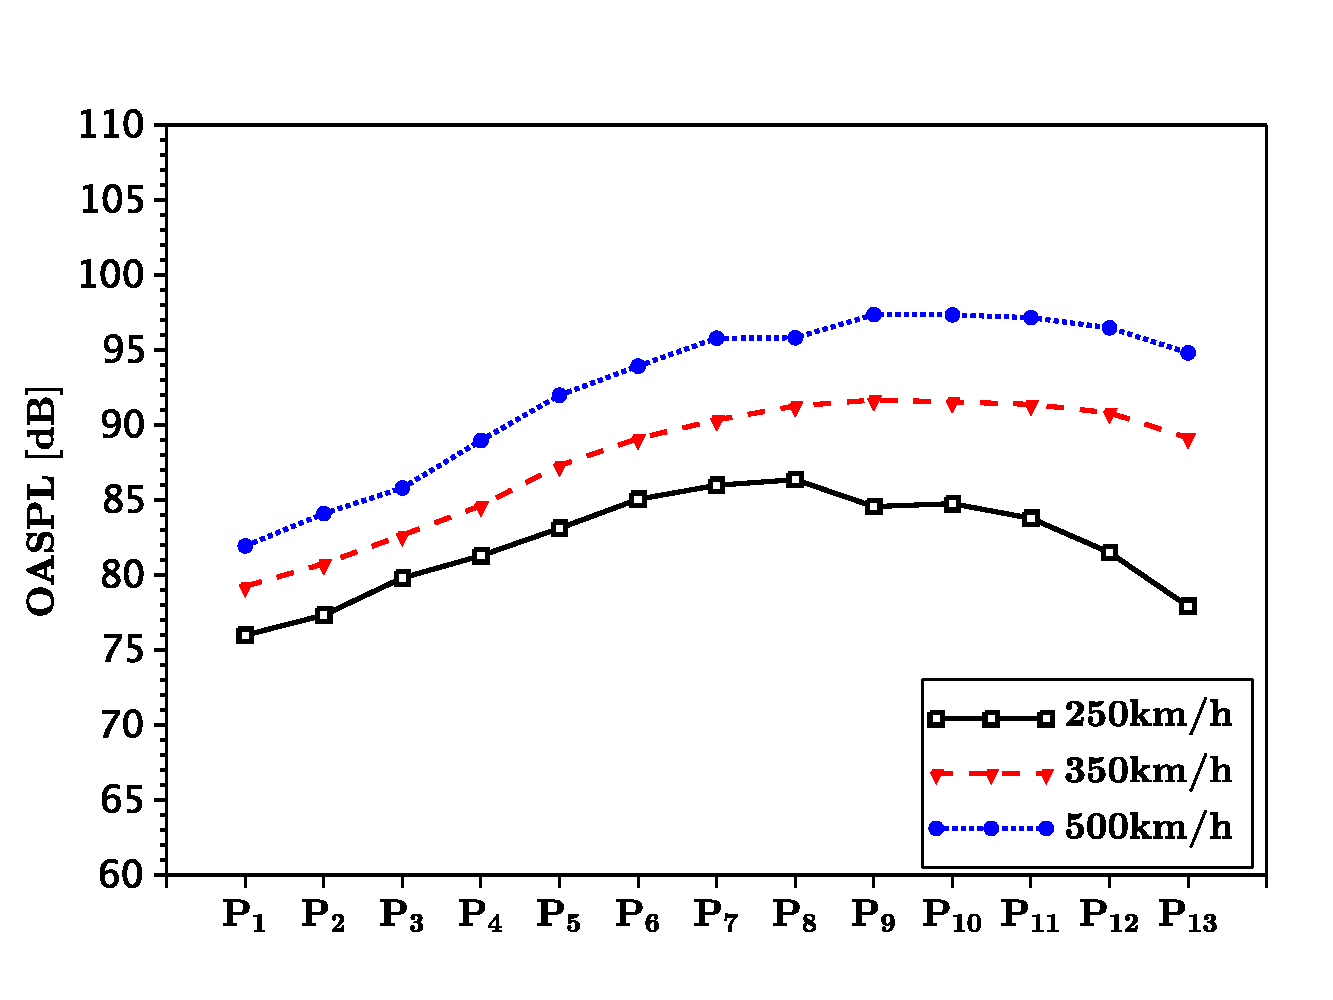
\includegraphics[width=\linewidth]{Figures/oaspl_c.pdf}
    \neusubfigcaption{fig:ch0-side-by-side-a}{工况一}
  \end{neusubfigure}
  \hfill
  \begin{neusubfigure}{0.49\linewidth}
    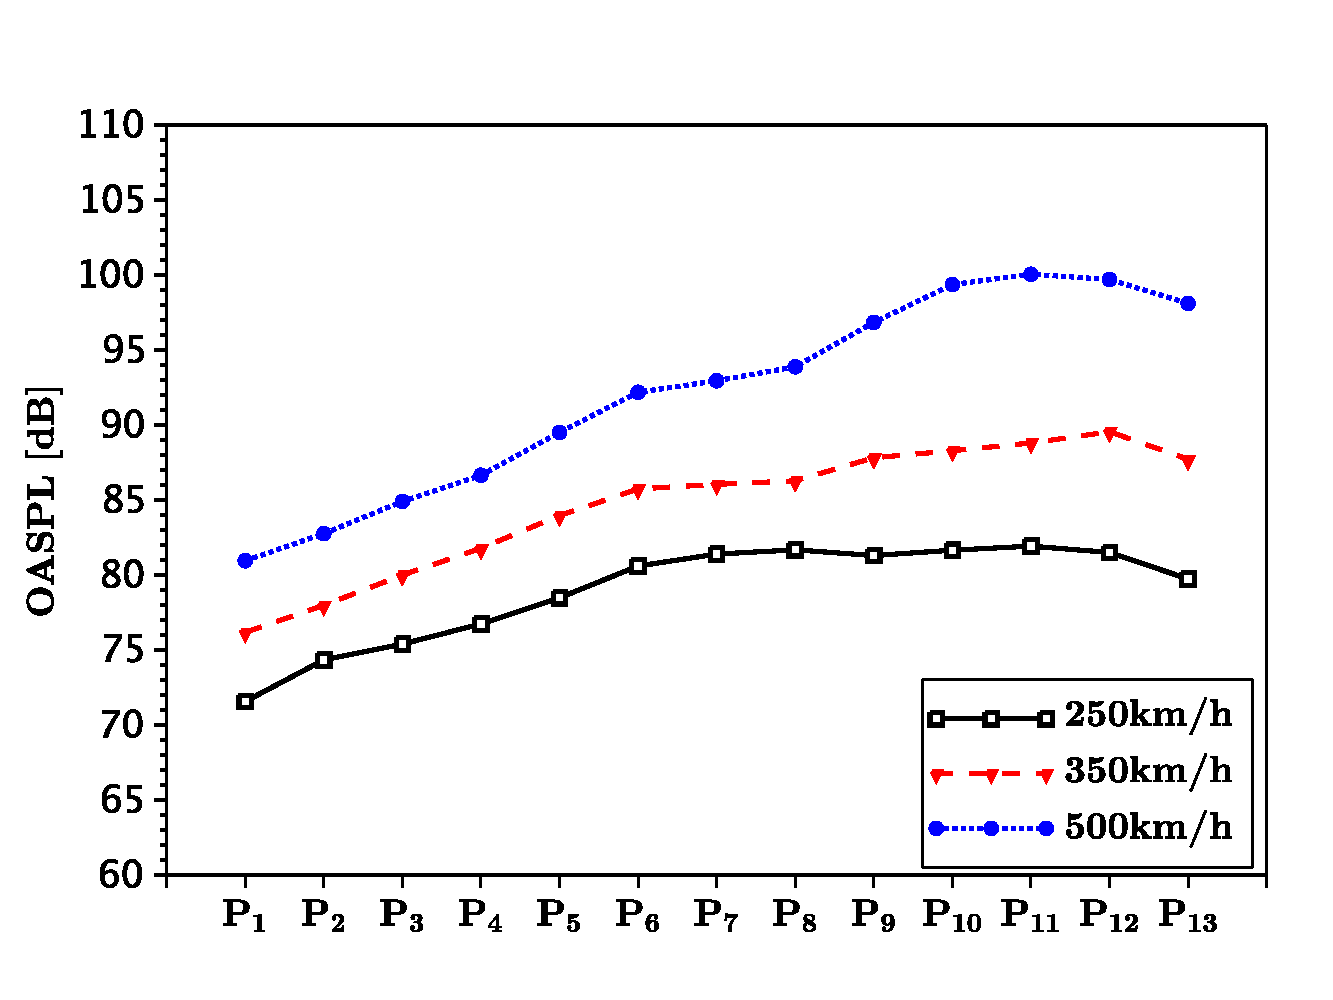
\includegraphics[width=\linewidth]{Figures/oaspl_d.pdf}
    \neusubfigcaption{fig:ch0-side-by-side-b}{工况二}
  \end{neusubfigure}
  \neufigcaption{fig:ch0-subfigures}{并列子图排版样例}{Example of Side-by-Side Subfigures}
\end{figure}

\neufigref{fig:ch0-subfigures} 使用 \texttt{neusubfigure} 完成并列子图排版。
其中 \neusubfigref{fig:ch0-side-by-side-a} 和 \neusubfigref{fig:ch0-side-by-side-b} 可分别引用到子图。
当两幅图共享一个总标题且需要分别引用时，可使用这种方式；如果每幅图需要完全独立的图号，建议拆成两个独立的 \texttt{figure} 环境。

\subsection{二乘二子图}
\begin{figure}[!htbp]
  \centering
  \begin{neusubfigure}{0.49\linewidth}
    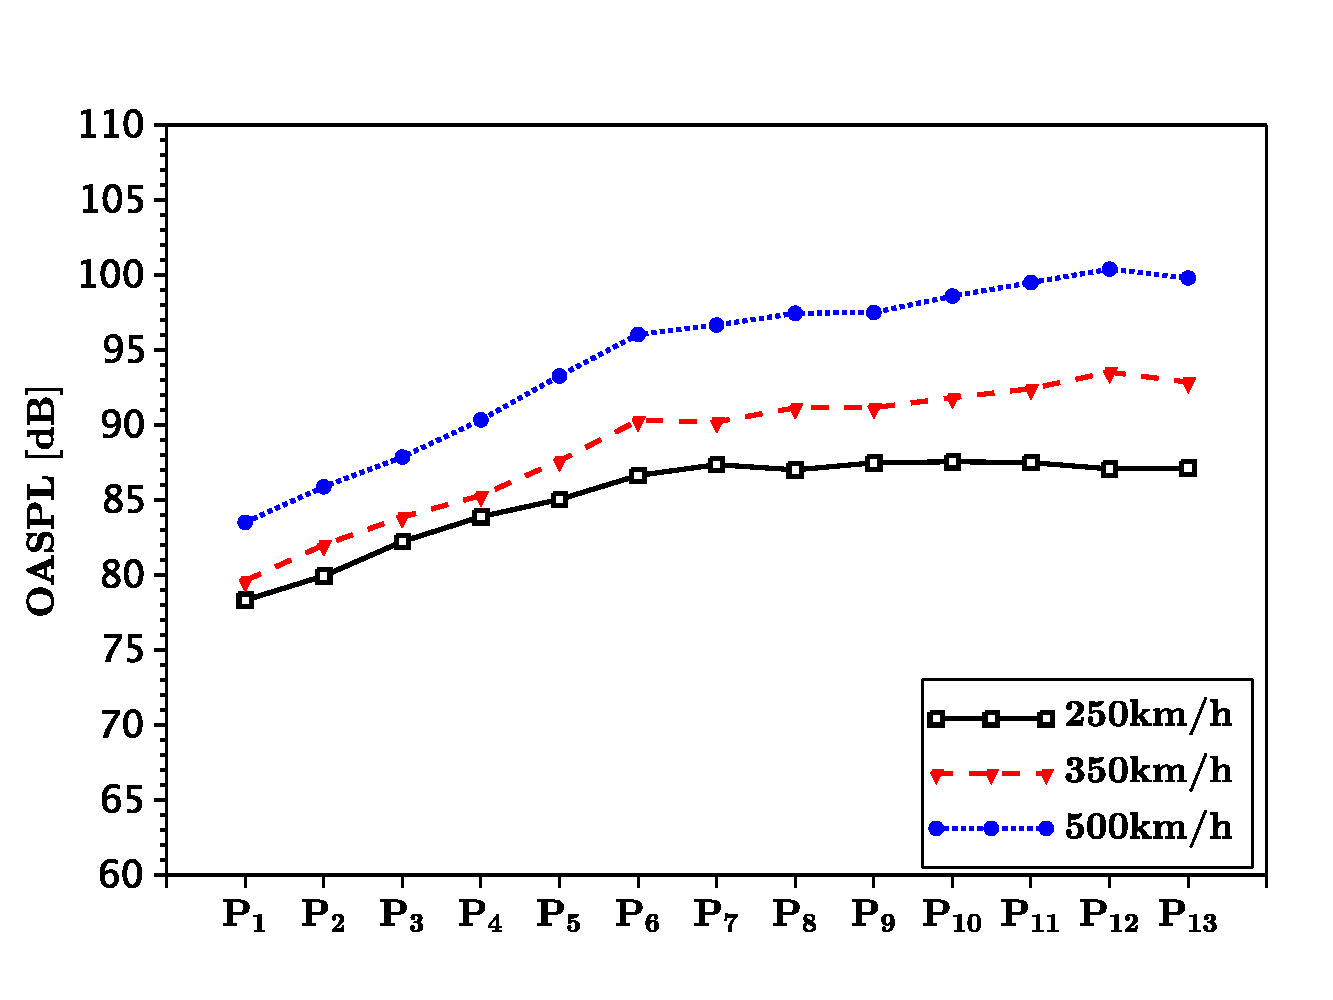
\includegraphics[width=\linewidth]{Figures/oaspl_a.pdf}
    \neusubfigcaption{fig:ch0-four-subfig-a}{工况一}
  \end{neusubfigure}
  \hfill
  \begin{neusubfigure}{0.49\linewidth}
    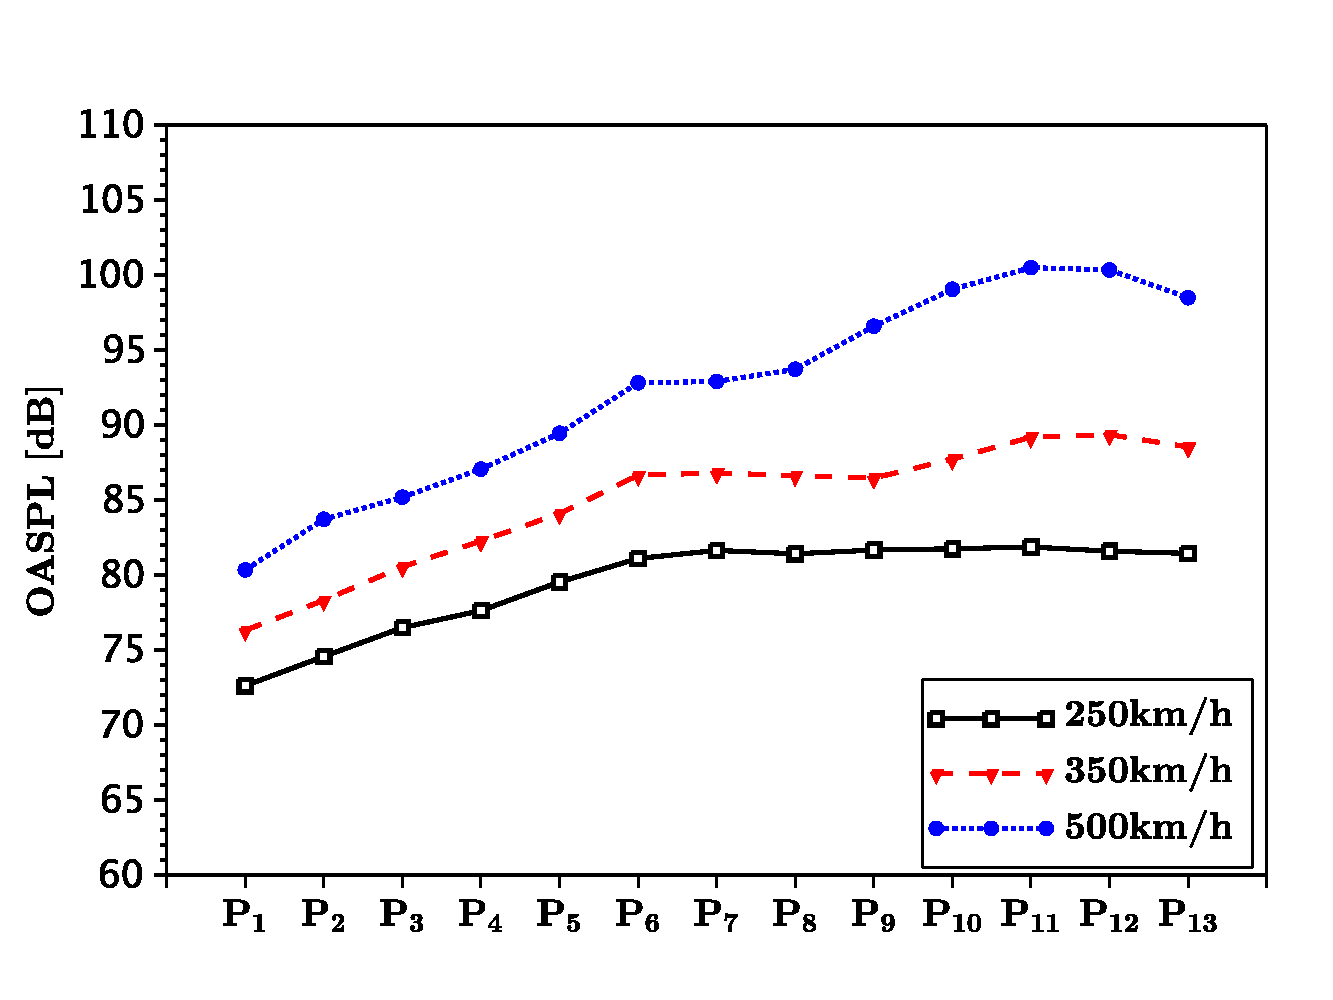
\includegraphics[width=\linewidth]{Figures/oaspl_b.pdf}
    \neusubfigcaption{fig:ch0-four-subfig-b}{工况二}
  \end{neusubfigure}
  \par\vspace{2bp}

  \begin{neusubfigure}{0.49\linewidth}
    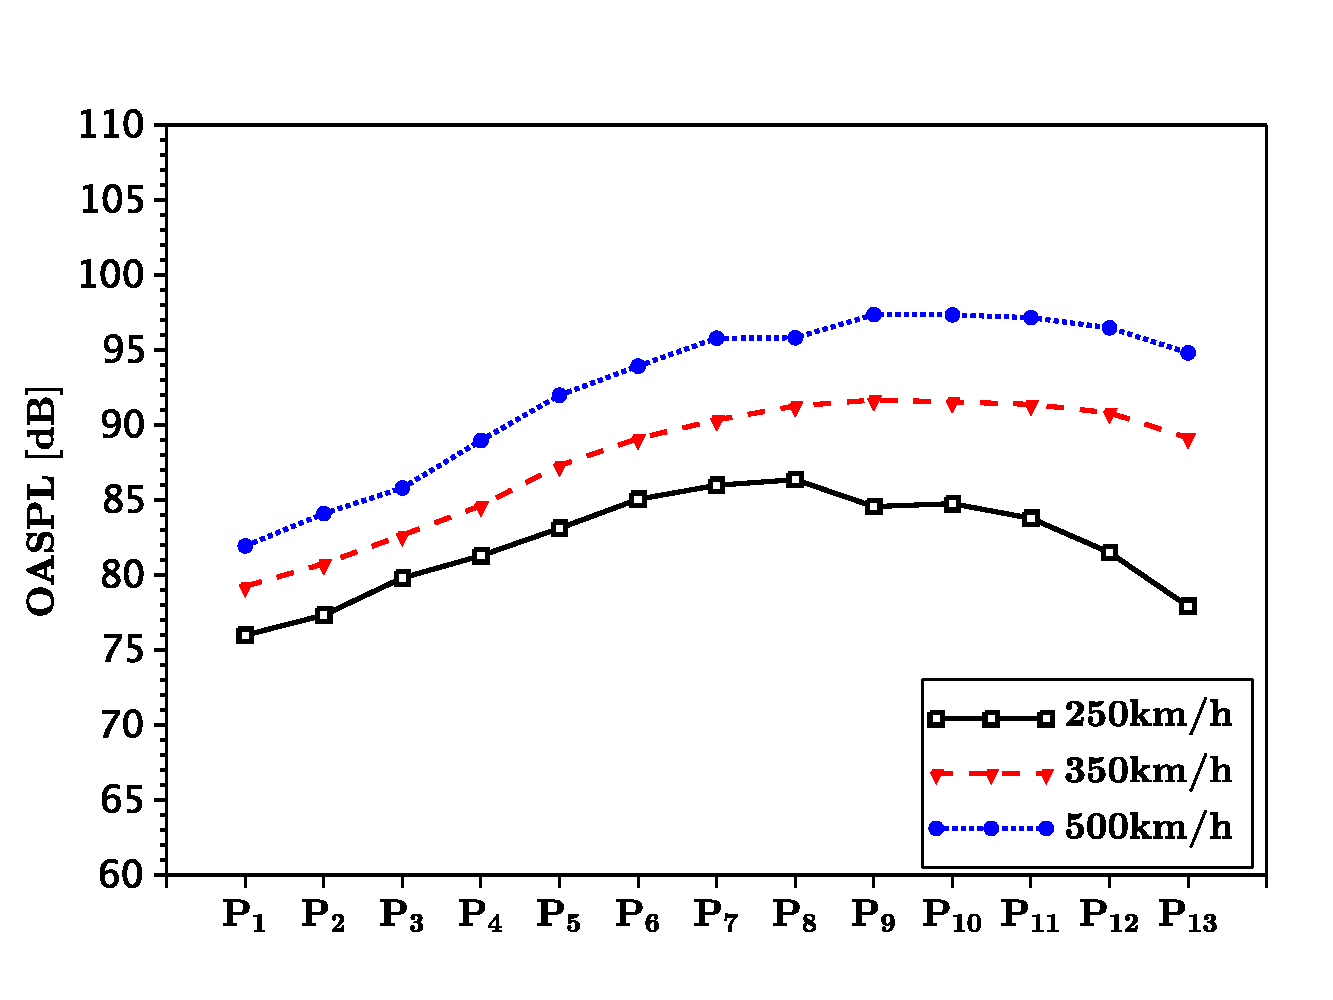
\includegraphics[width=\linewidth]{Figures/oaspl_c.pdf}
    \neusubfigcaption{fig:ch0-four-subfig-c}{工况三}
  \end{neusubfigure}
  \hfill
  \begin{neusubfigure}{0.49\linewidth}
    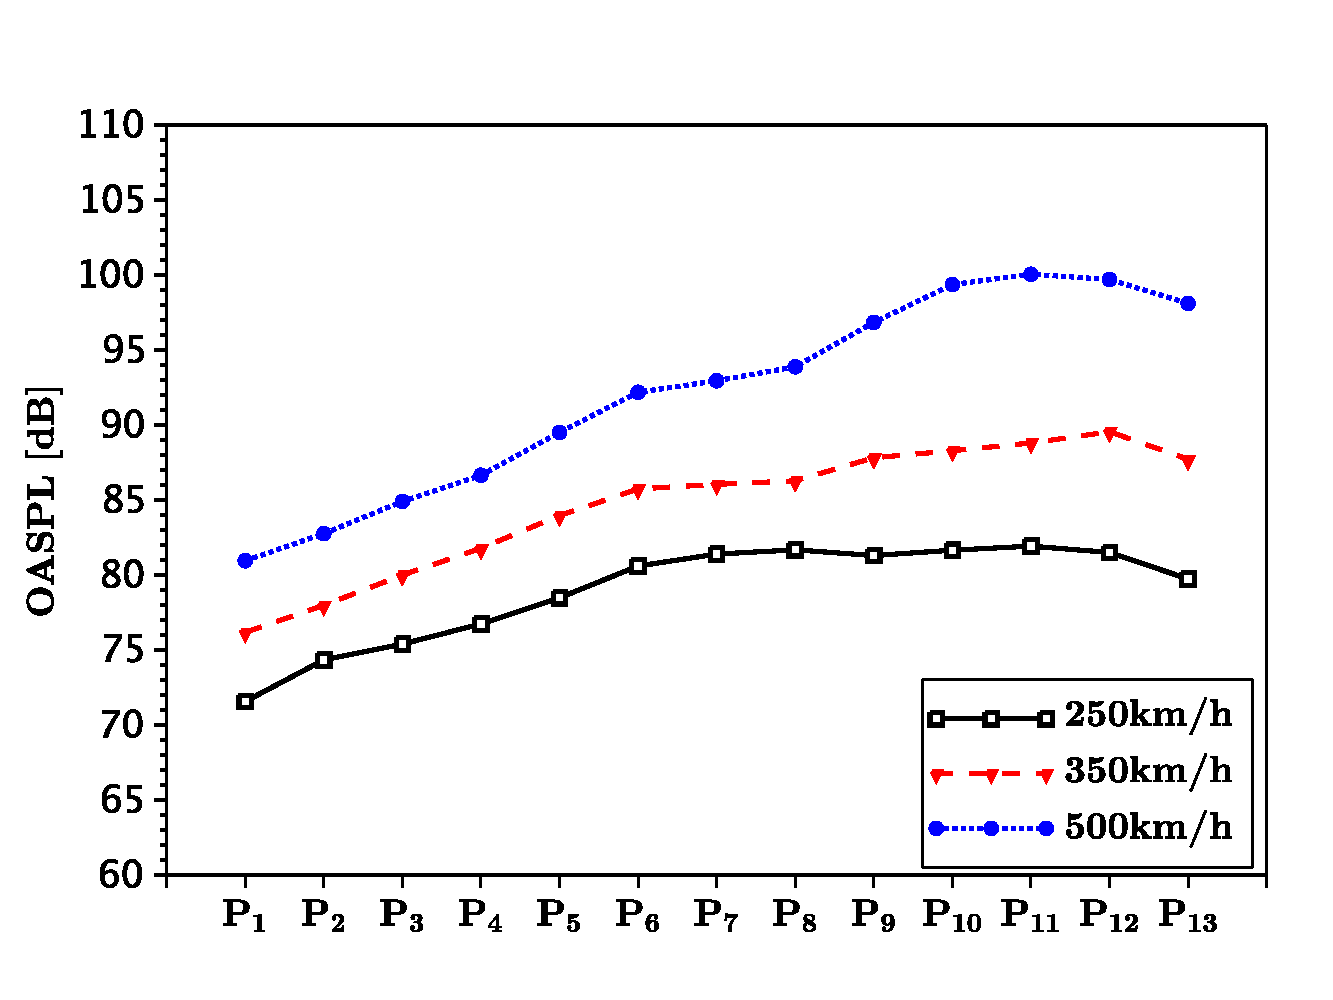
\includegraphics[width=\linewidth]{Figures/oaspl_d.pdf}
    \neusubfigcaption{fig:ch0-four-subfig-d}{工况四}
  \end{neusubfigure}
  \neufigcaption{fig:ch0-four-subfigures}{二乘二子图排版样例}{Example of Two-by-Two Subfigures}
\end{figure}

\neufigref{fig:ch0-four-subfigures} 展示了四幅子图的二乘二排布。
例如 \neusubfigref{fig:ch0-four-subfig-a} 至 \neusubfigref{fig:ch0-four-subfig-d} 可分别引用到四个子图。
排版时建议注意以下几点：
\begin{itemize}
  \item 子图宽度通常可取 \verb|0.48\linewidth| 至 \verb|0.49\linewidth|。
  \item 每行两个子图之间使用 \verb|\hfill| 自动拉开横向间距。
  \item 两行之间可用少量 \verb|\par\vspace| 控制垂直间距。
\end{itemize}

\section{表格排版}

本模板提供 \verb|\neutabcaption{label}{中文题名}{English title}| 用于生成中英文表题。
表题应置于表格上方，正文中使用 \verb|\neutabref{label}| 引用。
表格同样建议使用 \verb|[!htbp]|。如果表格过高导致页底空白，优先考虑缩小字号、调整列宽、拆分表格或使用跨页表格，而不是强制分页。

\subsection{三线表}

\begin{table}[!htbp]
  \centering
  \neutabcaption{tab:ch0-booktabs}{三线表样例}{Example of a Three-Line Table}
  \begin{tabular}{lccc}
    \toprule
    方法       & 准确率（\%）       & 召回率（\%）       & F1 值           \\
    \midrule
    Baseline & 85.2          & 84.1          & 0.846          \\
    Method A & 89.7          & 88.9          & 0.893          \\
    Proposed & \textbf{92.1} & \textbf{91.5} & \textbf{0.918} \\
    \bottomrule
  \end{tabular}
\end{table}

\neutabref{tab:ch0-booktabs} 展示了推荐的三线表格式。
论文中应尽量避免过多竖线，以保持表格简洁。

\subsection{复杂表格}
\begin{table}[!htbp]
  \centering
  \neutabcaption{tab:ch0-complex}{合并单元格与自动换行表格样例}{Example of Merged Cells and Auto-Wrapping Columns}
  \begin{tabularx}{\textwidth}{llXc}
    \toprule
    类别                  & 指标  & 说明                               & 是否必需 \\
    \midrule
    \multirow{2}{*}{图形} & 分辨率 & 位图图片应保证在最终 PDF 中清晰可辨。            & 是    \\
                        & 题名  & 图题使用中英文双语标题，并位于图片下方。             & 是    \\
    \midrule
    \multirow{2}{*}{表格} & 宽度  & 宽表格可使用 \texttt{tabularx} 自动分配列宽。 & 否    \\
                        & 表注  & 表内说明应简明，必要时可在正文中解释。              & 否    \\
    \bottomrule
  \end{tabularx}
\end{table}

\neutabref{tab:ch0-complex} 同时展示了 \verb|\multirow|、\verb|\makecell| 可配合使用的复杂表格场景。
若单元格内容较长，优先使用 \texttt{tabularx} 或 \texttt{p\{...\}} 列类型控制宽度。

\section{公式排版}

公式应使用标准数学环境，并通过 \verb|\label| 设置标签。
引用公式时建议使用模板提供的 \verb|\neueqref{label}|。

\subsection{单行公式}
以分类任务中的交叉熵损失为例，可写为
\begin{equation}
  \mathcal{L}(\theta)
  = - \frac{1}{N}\sum_{i=1}^{N}\sum_{k=1}^{K} y_{ik}\log p_{ik}
  \label{eq:ch0-loss}
\end{equation}

如 \neueqref{eq:ch0-loss} 所示，带编号公式适合放置正文中需要引用的重要定义。

\subsection{多行公式}
循环模型中的状态更新和输出计算可写为
\begin{align}
  h_t       & = \sigma(W_x x_t + W_h h_{t-1} + b), \label{eq:ch0-state} \\
  \hat{y}_t & = \operatorname{softmax}(W_o h_t). \label{eq:ch0-output}
\end{align}

\neueqref{eq:ch0-state} 和 \neueqref{eq:ch0-output} 展示了多行公式的编号方式。
如果多行推导只需要一个编号，可使用 \texttt{aligned} 放在 \texttt{equation} 环境内部。

\subsection{分段函数与矩阵}
分段函数和矩阵经常同时出现在数学定义中，例如
\begin{equation}
  g(x)=
  \begin{cases}
    0, & x < 0,       \\
    x, & 0 \le x < 1, \\
    1, & x \ge 1,
  \end{cases}
  \qquad
  A =
  \begin{bmatrix}
    1 & 0 & 0 \\
    0 & 1 & 0 \\
    0 & 0 & 1
  \end{bmatrix}.
  \label{eq:ch0-piecewise}
\end{equation}

\neueqref{eq:ch0-piecewise} 展示了分段函数和矩阵的常见写法。

\section{算法伪代码}

计算机类论文常需要给出算法步骤。本文档在 \texttt{main.tex} 中加载了 \texttt{algorithm} 和 \texttt{algorithmic} 宏包，可以直接使用如下环境。

\begin{algorithm}[!htbp]
  \caption{样例训练流程}
  \label{alg:ch0-training}
  \begin{algorithmic}[1]
    \REQUIRE Training set $\mathcal{D}$, learning rate $\eta$, maximum epoch $T$
    \ENSURE Model parameters $\theta$
    \STATE Initialize parameters $\theta$
    \FOR{$t = 1$ to $T$}
    \STATE Sample a mini-batch $\mathcal{B}$ from $\mathcal{D}$
    \STATE Compute loss $\mathcal{L}(\theta)$ by \neueqref{eq:ch0-loss}
    \STATE Update $\theta \leftarrow \theta - \eta \nabla_{\theta}\mathcal{L}(\theta)$
    \ENDFOR
    \RETURN $\theta$
  \end{algorithmic}
\end{algorithm}

算法~\ref{alg:ch0-training} 展示了带行号的伪代码。
若需要中文关键字，可在导言区重定义相应命令。

\section{引用、链接与交叉引用}

参考文献引用可使用两种模板命令：
\begin{itemize}
  \item 上标引用使用 \verb|\upcite{key}|，适合放在句末，例如已有研究讨论了神经网络轻量化问题\upcite{guo_2023_research}。
  \item 正文引用使用 \verb|\inlinecite{key}|，适合作为句子成分，例如文献 \inlinecite{thakkar_2018_performance} 给出了系统性能评测案例。
\end{itemize}
多篇文献可写在同一条引用命令中，例如区块链平台相关研究\upcite{zheng_2019_nutbaas,thakkar_2018_performance}。

交叉引用建议统一使用模板命令：
\begin{itemize}
  \item 图引用：\verb|\neufigref{fig:ch0-pdf}|，效果为 \neufigref{fig:ch0-pdf}。
  \item 子图引用：\verb|\neusubfigref{fig:ch0-four-subfig-a}|，效果为 \neusubfigref{fig:ch0-four-subfig-a}。
  \item 表引用：\verb|\neutabref{tab:ch0-complex}|，效果为 \neutabref{tab:ch0-complex}。
  \item 公式引用：\verb|\neueqref{eq:ch0-loss}|，效果为 \neueqref{eq:ch0-loss}。
  \item 算法引用：当前模板未单独封装算法引用命令，可写作“算法~\ref{alg:ch0-training}”。
\end{itemize}
模板提供的公开命令和环境可参考 \texttt{README.md} 中的“模板命令说明”一节。
|。
脚注示例如此处所示\footnote{脚注用于补充说明，不宜放置过长的正文内容。}。
若某页因图表浮动或分页规则没有排满，脚注可能跟随正文排版区而显得略高，这是正常的 LaTeX 页面构建结果。

\subsection{字体、字号与强调}

模板预定义了常用中文字体命令。正式论文中通常不需要手动切换字体；只有在展示样式、术语强调或特殊说明时才建议使用。
当前模板已经为默认宋体和 \verb|\song| 字族配置伪粗体，因此 \verb|\textbf| 或 \verb|\bfseries| 可以用于中文局部强调。
需要注意的是，中文加粗应克制使用；标题层级、术语定义或表格重点值可以适当加粗，大段正文不建议整体加粗。
如果需要更明显的标题式强调，可使用黑体或调整标题层级；如果只是普通正文重点，优先使用 \verb|\textbf|。

\begin{table}[!htbp]
  \centering
  \neutabcaption{tab:ch0-fonts}{字体与强调样例}{Examples of Fonts and Emphasis}
  \begin{tabular}{lll}
    \toprule
    命令             & 显示效果                         & 使用建议       \\
    \midrule
    \verb|\song|   & {\song 宋体文字示例}               & 正文默认字体     \\
    \verb|\textbf| & \textbf{加粗文字示例}              & 局部强调、表格重点值 \\
    \verb|\hei|    & {\hei 黑体文字示例}                & 标题或较强强调场景  \\
    \verb|\kai|    & {\kai 楷体文字示例}                & 摘要、题签或引用语  \\
    \verb|\fs|     & {\fs 仿宋文字示例}                 & 特殊文书类内容    \\
    \verb|\textit| & \textit{Italic text example} & 英文斜体或变量说明  \\
    \bottomrule
  \end{tabular}
\end{table}

\subsection{列表环境}

无序列表适合列出并列事项：
\begin{itemize}
  \item 图题位于图下方，表题位于表上方。
  \item 图表应使用中英文双语标题。
  \item 公式、图、表、算法均应使用标签进行交叉引用。
\end{itemize}

有序列表适合描述步骤：
\begin{enumerate}
  \item 在 \texttt{main.tex} 中填写论文元信息。
  \item 在各章文件中撰写正文内容。
  \item 使用 \texttt{latexmk -xelatex main.tex} 完成编译。
\end{enumerate}

\section{图形排版}

本模板提供 \verb|\neufigcaption{label}{中文题名}{English title}| 用于生成中英文图题。
图题应置于图形下方，正文中使用 \verb|\neufigref{label}| 引用。
图形建议使用 \verb|[!htbp]| 浮动参数，让 LaTeX 在当前位置、页顶、页底或浮动页中选择较合适的位置；除非必须固定位置，否则不建议使用 \verb|[H]|。

\subsection{外部图片}
\begin{figure}[!htbp]
  \centering
  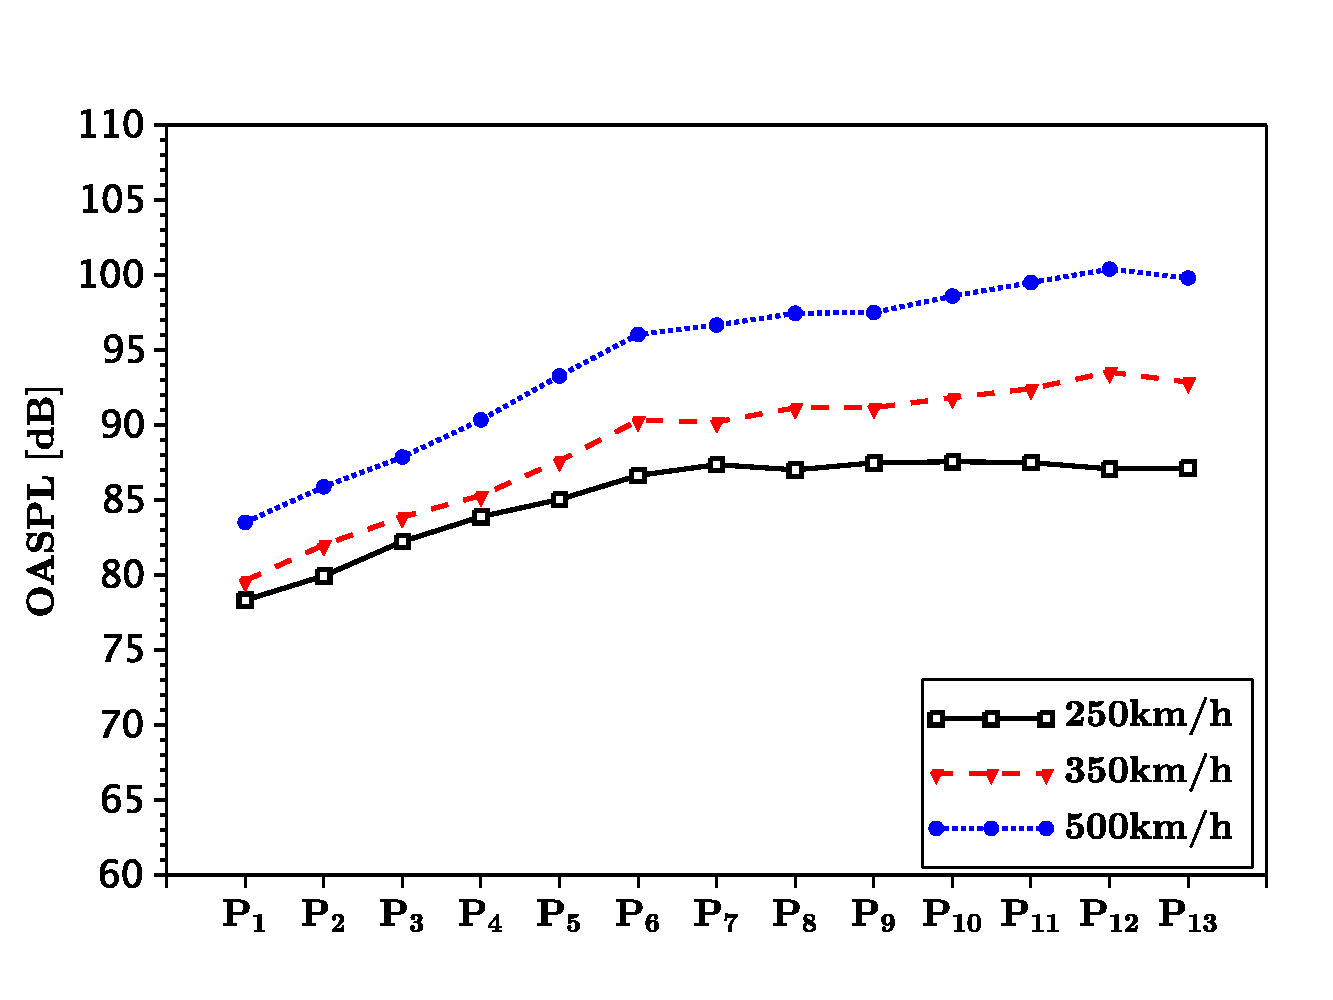
\includegraphics[width=0.55\textwidth]{Figures/oaspl_a.pdf}
  \neufigcaption{fig:ch0-cover}{外部图片插入样例}{Example of Including an External Image}
\end{figure}

\neufigref{fig:ch0-cover} 展示了通过 \verb|\includegraphics| 插入图片文件的方式。
正式论文中建议将图片统一放入 \texttt{Figures} 目录，并使用相对路径引用。

\subsection{PDF 或位图图片}
\begin{figure}[!htbp]
  \centering
  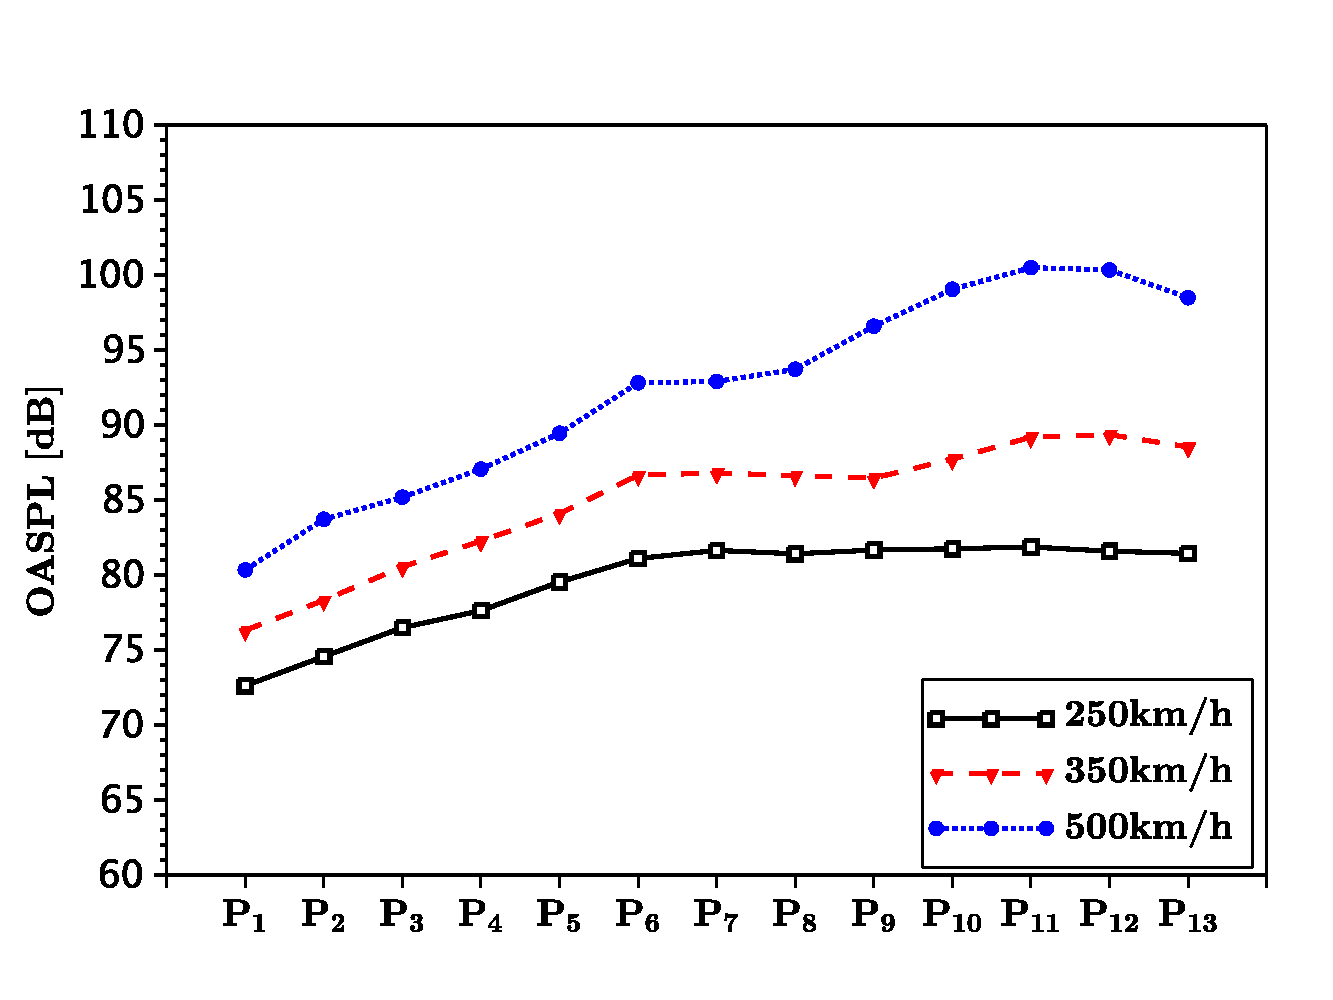
\includegraphics[width=0.55\textwidth]{Figures/oaspl_b.pdf}
  \neufigcaption{fig:ch0-pdf}{PDF 图片插入样例}{Example of Including a PDF Figure}
\end{figure}

PDF、PNG、JPG 等常见图片格式均可通过 \verb|\includegraphics| 插入。
若图片由绘图软件或数据分析程序导出，建议优先使用 PDF 格式以保持较清晰的显示效果。

\subsection{并列图片}
\begin{figure}[!htbp]
  \centering
  \begin{minipage}[t]{0.49\linewidth}
    \centering
    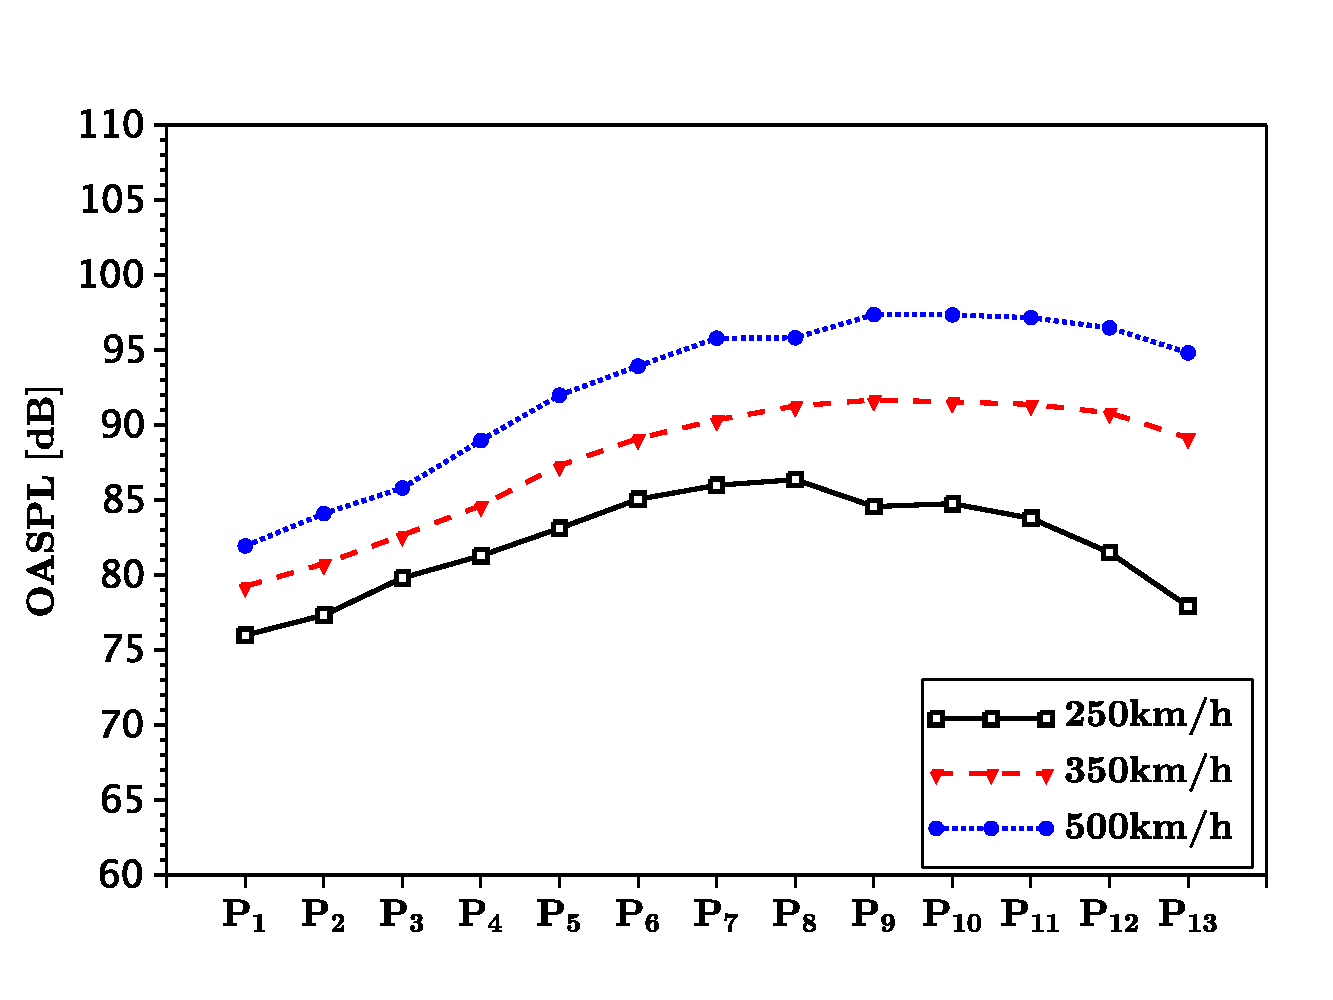
\includegraphics[width=\linewidth]{Figures/oaspl_c.pdf}
  \end{minipage}
  \hfill
  \begin{minipage}[t]{0.49\linewidth}
    \centering
    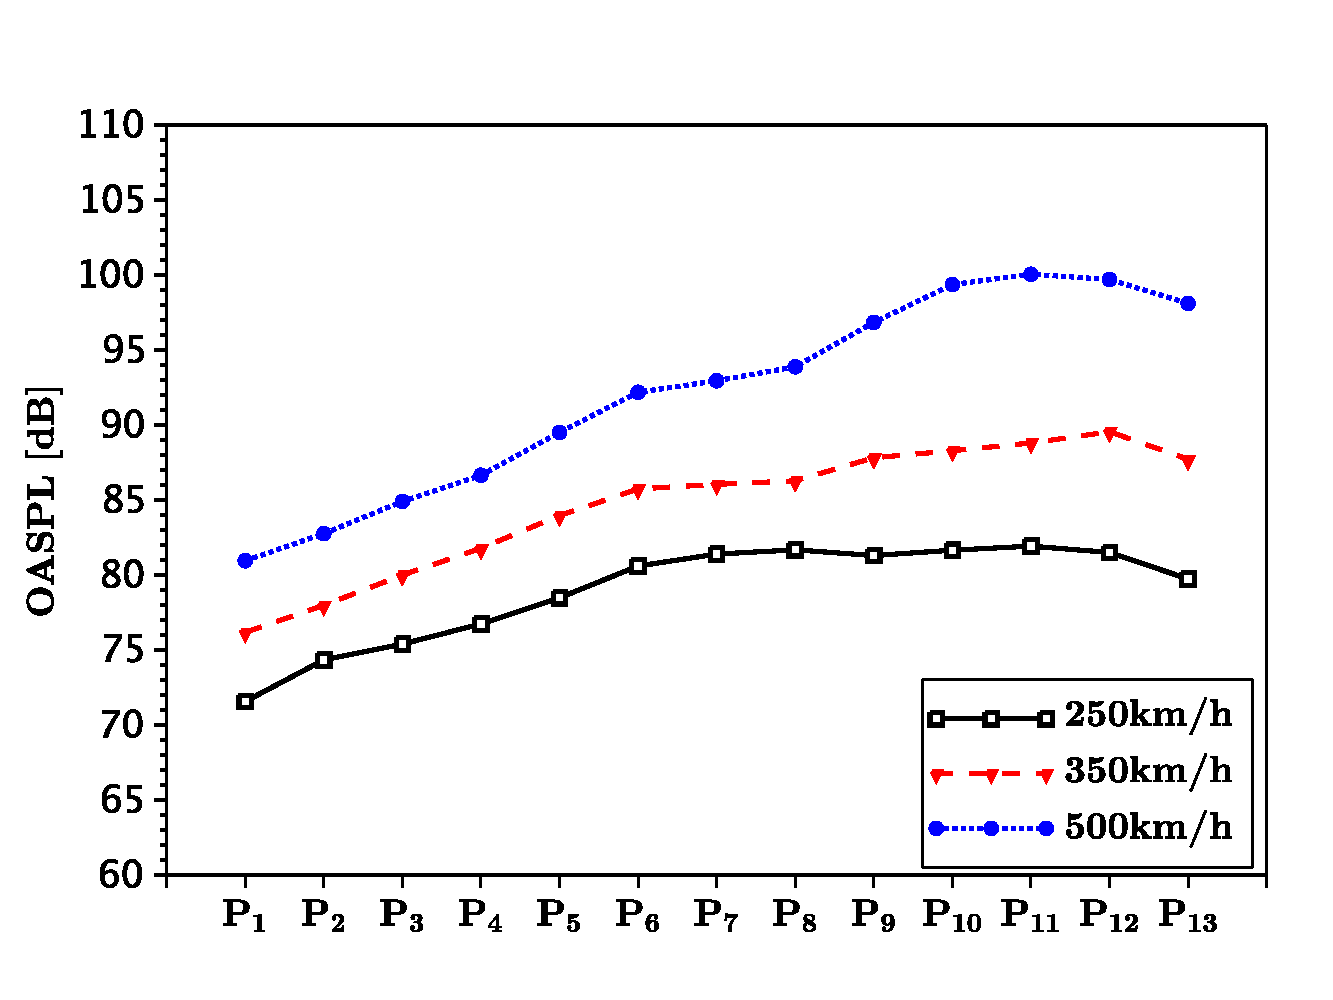
\includegraphics[width=\linewidth]{Figures/oaspl_d.pdf}
  \end{minipage}
  \neufigcaption{fig:ch0-side-by-side}{普通并列图形排版样例}{Example of Side-by-Side Figures}
\end{figure}

\neufigref{fig:ch0-side-by-side} 使用 \texttt{minipage} 完成普通并列排版。
当两幅图共享一个总标题且不需要分别引用时，可使用这种方式。

\subsection{并列子图}
\begin{figure}[!htbp]
  \centering
  \begin{neusubfigure}{0.49\linewidth}
    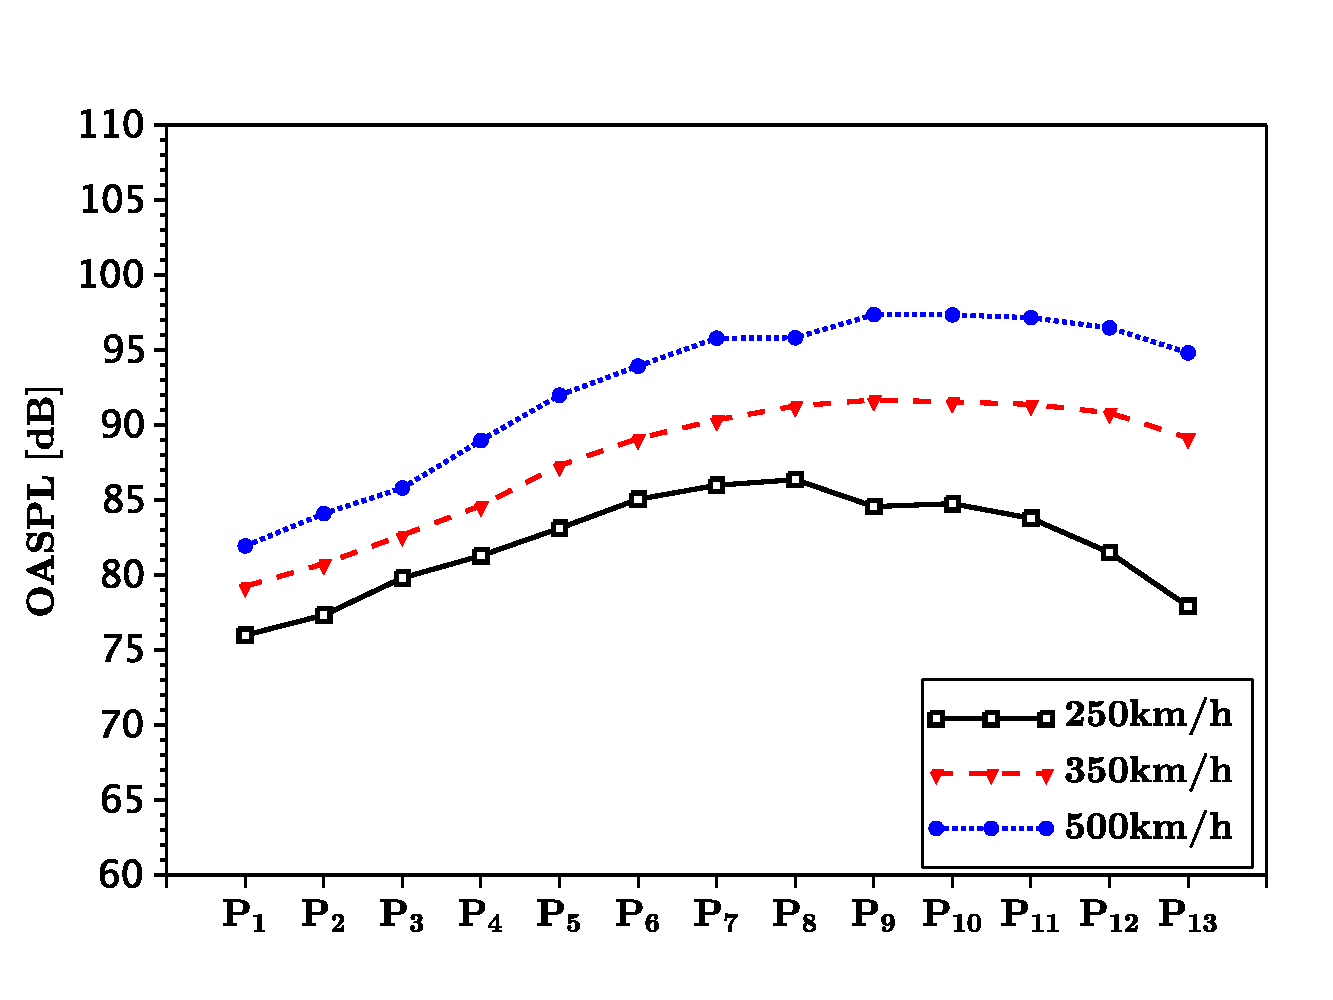
\includegraphics[width=\linewidth]{Figures/oaspl_c.pdf}
    \neusubfigcaption{fig:ch0-side-by-side-a}{工况一}
  \end{neusubfigure}
  \hfill
  \begin{neusubfigure}{0.49\linewidth}
    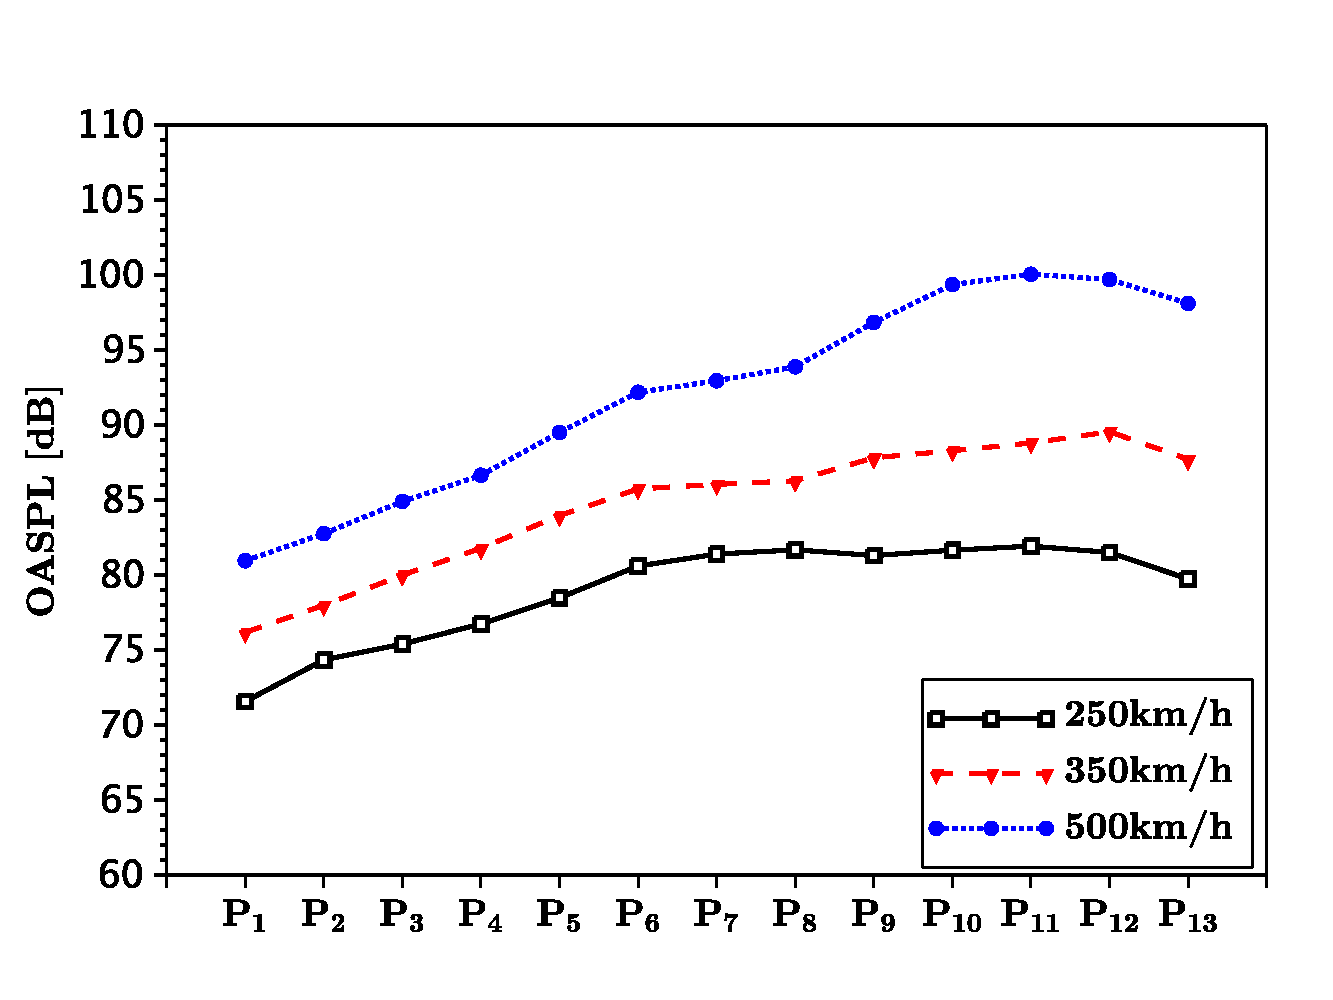
\includegraphics[width=\linewidth]{Figures/oaspl_d.pdf}
    \neusubfigcaption{fig:ch0-side-by-side-b}{工况二}
  \end{neusubfigure}
  \neufigcaption{fig:ch0-subfigures}{并列子图排版样例}{Example of Side-by-Side Subfigures}
\end{figure}

\neufigref{fig:ch0-subfigures} 使用 \texttt{neusubfigure} 完成并列子图排版。
其中 \neusubfigref{fig:ch0-side-by-side-a} 和 \neusubfigref{fig:ch0-side-by-side-b} 可分别引用到子图。
当两幅图共享一个总标题且需要分别引用时，可使用这种方式；如果每幅图需要完全独立的图号，建议拆成两个独立的 \texttt{figure} 环境。

\subsection{二乘二子图}
\begin{figure}[!htbp]
  \centering
  \begin{neusubfigure}{0.49\linewidth}
    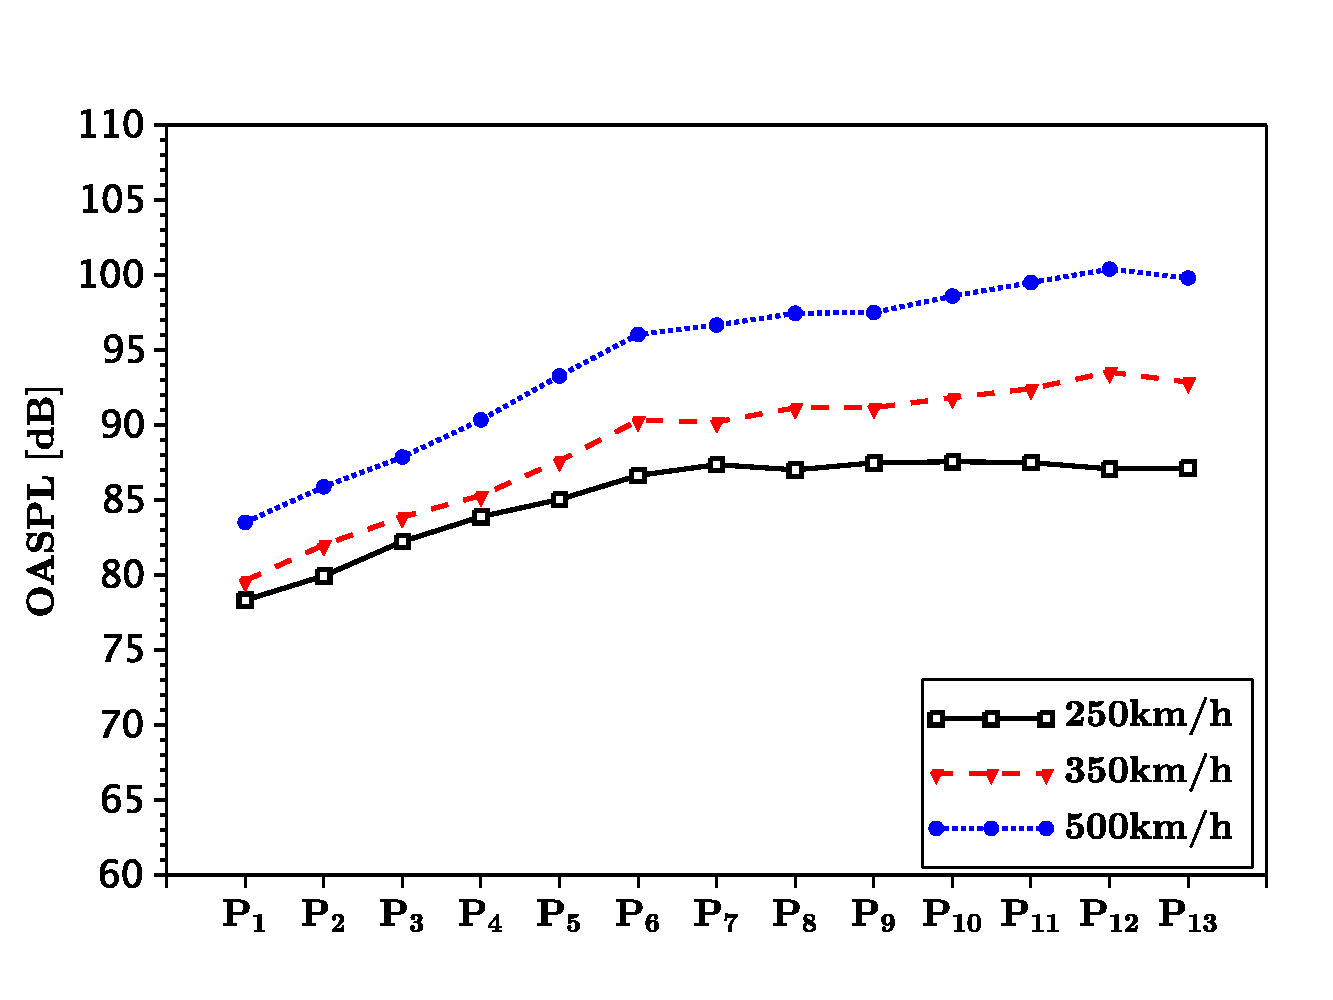
\includegraphics[width=\linewidth]{Figures/oaspl_a.pdf}
    \neusubfigcaption{fig:ch0-four-subfig-a}{工况一}
  \end{neusubfigure}
  \hfill
  \begin{neusubfigure}{0.49\linewidth}
    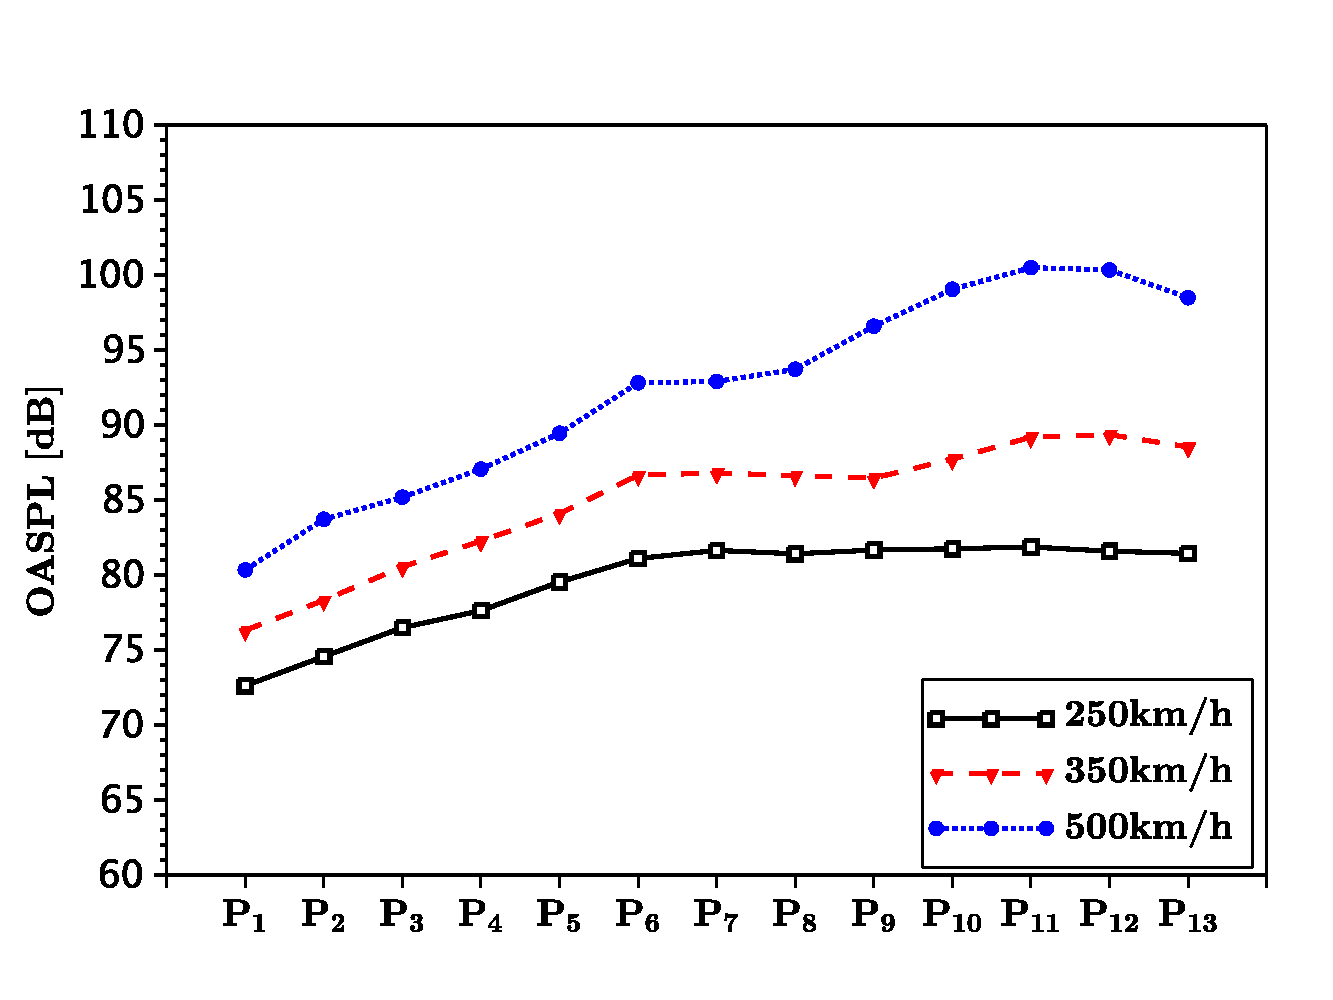
\includegraphics[width=\linewidth]{Figures/oaspl_b.pdf}
    \neusubfigcaption{fig:ch0-four-subfig-b}{工况二}
  \end{neusubfigure}
  \par\vspace{2bp}

  \begin{neusubfigure}{0.49\linewidth}
    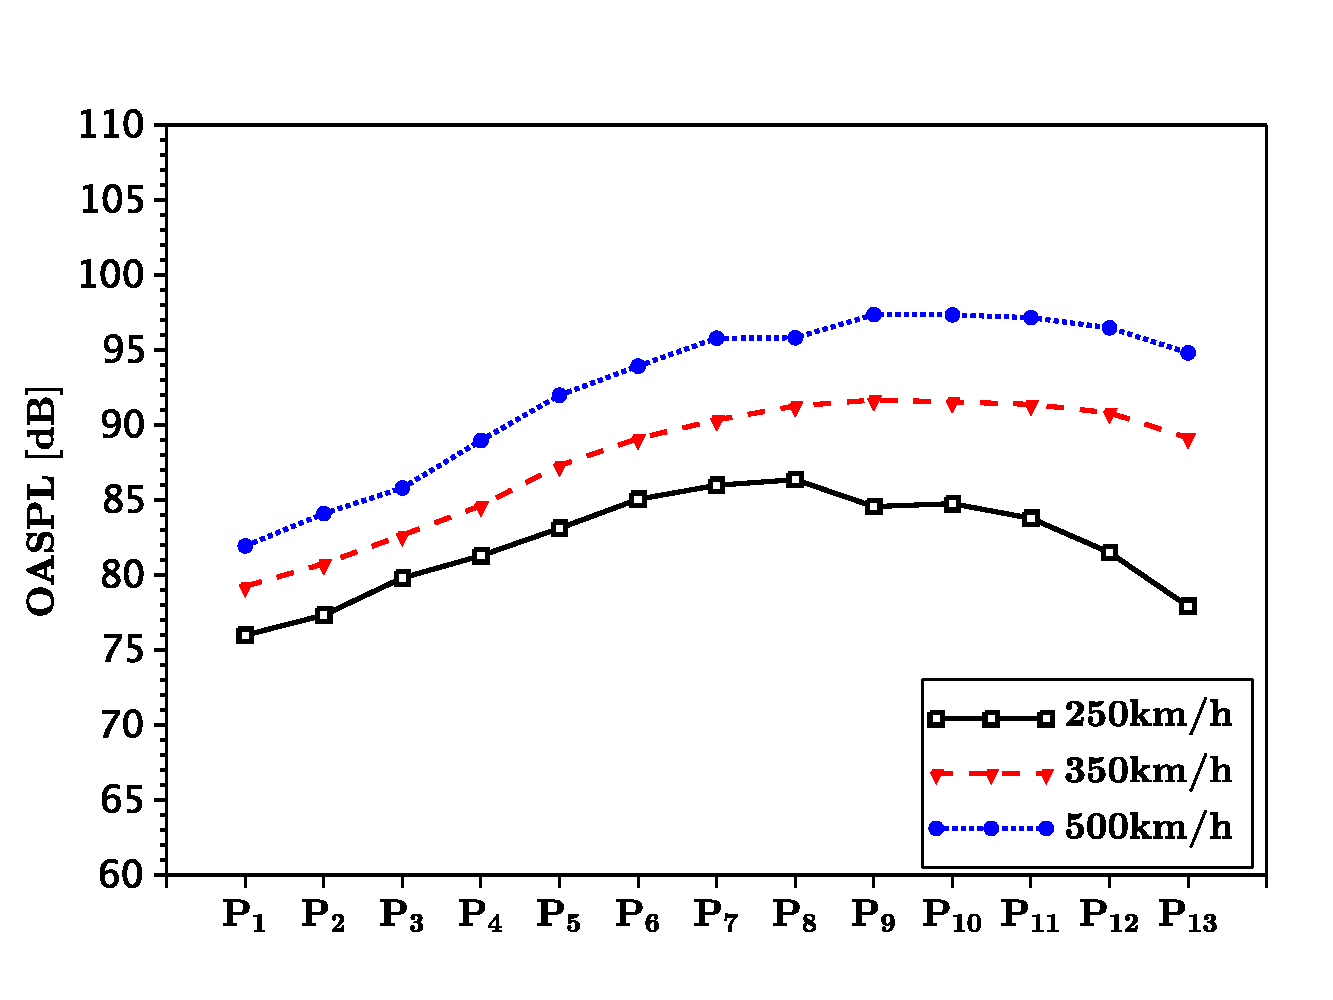
\includegraphics[width=\linewidth]{Figures/oaspl_c.pdf}
    \neusubfigcaption{fig:ch0-four-subfig-c}{工况三}
  \end{neusubfigure}
  \hfill
  \begin{neusubfigure}{0.49\linewidth}
    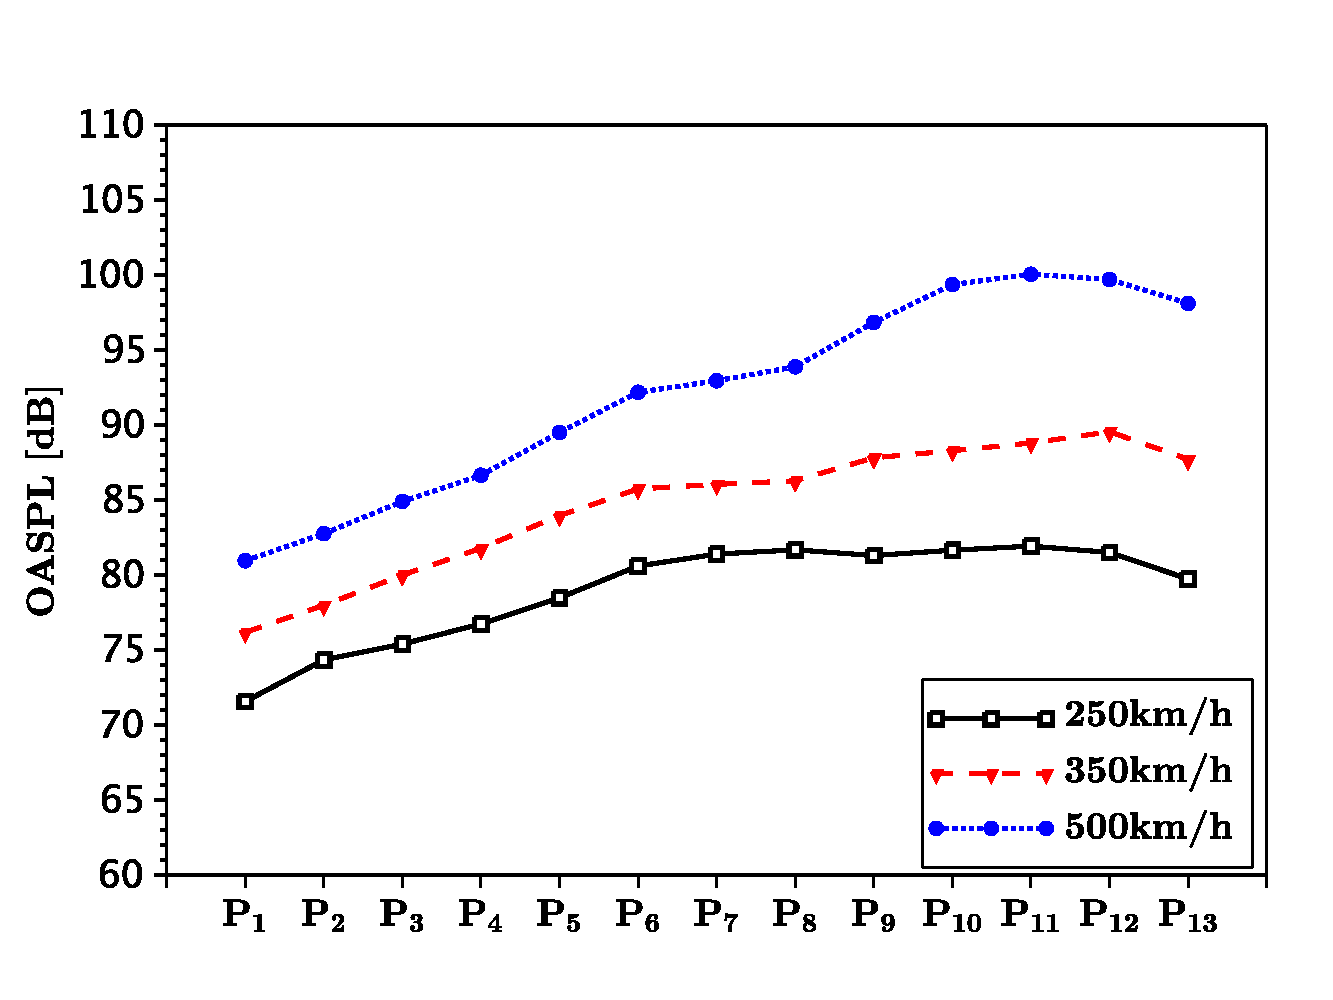
\includegraphics[width=\linewidth]{Figures/oaspl_d.pdf}
    \neusubfigcaption{fig:ch0-four-subfig-d}{工况四}
  \end{neusubfigure}
  \neufigcaption{fig:ch0-four-subfigures}{二乘二子图排版样例}{Example of Two-by-Two Subfigures}
\end{figure}

\neufigref{fig:ch0-four-subfigures} 展示了四幅子图的二乘二排布。
例如 \neusubfigref{fig:ch0-four-subfig-a} 至 \neusubfigref{fig:ch0-four-subfig-d} 可分别引用到四个子图。
排版时建议注意以下几点：
\begin{itemize}
  \item 子图宽度通常可取 \verb|0.48\linewidth| 至 \verb|0.49\linewidth|。
  \item 每行两个子图之间使用 \verb|\hfill| 自动拉开横向间距。
  \item 两行之间可用少量 \verb|\par\vspace| 控制垂直间距。
\end{itemize}

\section{表格排版}

本模板提供 \verb|\neutabcaption{label}{中文题名}{English title}| 用于生成中英文表题。
表题应置于表格上方，正文中使用 \verb|\neutabref{label}| 引用。
表格同样建议使用 \verb|[!htbp]|。如果表格过高导致页底空白，优先考虑缩小字号、调整列宽、拆分表格或使用跨页表格，而不是强制分页。

\subsection{三线表}

\begin{table}[!htbp]
  \centering
  \neutabcaption{tab:ch0-booktabs}{三线表样例}{Example of a Three-Line Table}
  \begin{tabular}{lccc}
    \toprule
    方法       & 准确率（\%）       & 召回率（\%）       & F1 值           \\
    \midrule
    Baseline & 85.2          & 84.1          & 0.846          \\
    Method A & 89.7          & 88.9          & 0.893          \\
    Proposed & \textbf{92.1} & \textbf{91.5} & \textbf{0.918} \\
    \bottomrule
  \end{tabular}
\end{table}

\neutabref{tab:ch0-booktabs} 展示了推荐的三线表格式。
论文中应尽量避免过多竖线，以保持表格简洁。

\subsection{复杂表格}
\begin{table}[!htbp]
  \centering
  \neutabcaption{tab:ch0-complex}{合并单元格与自动换行表格样例}{Example of Merged Cells and Auto-Wrapping Columns}
  \begin{tabularx}{\textwidth}{llXc}
    \toprule
    类别                  & 指标  & 说明                               & 是否必需 \\
    \midrule
    \multirow{2}{*}{图形} & 分辨率 & 位图图片应保证在最终 PDF 中清晰可辨。            & 是    \\
                        & 题名  & 图题使用中英文双语标题，并位于图片下方。             & 是    \\
    \midrule
    \multirow{2}{*}{表格} & 宽度  & 宽表格可使用 \texttt{tabularx} 自动分配列宽。 & 否    \\
                        & 表注  & 表内说明应简明，必要时可在正文中解释。              & 否    \\
    \bottomrule
  \end{tabularx}
\end{table}

\neutabref{tab:ch0-complex} 同时展示了 \verb|\multirow|、\verb|\makecell| 可配合使用的复杂表格场景。
若单元格内容较长，优先使用 \texttt{tabularx} 或 \texttt{p\{...\}} 列类型控制宽度。

\section{公式排版}

公式应使用标准数学环境，并通过 \verb|\label| 设置标签。
引用公式时建议使用模板提供的 \verb|\neueqref{label}|。

\subsection{单行公式}
以分类任务中的交叉熵损失为例，可写为
\begin{equation}
  \mathcal{L}(\theta)
  = - \frac{1}{N}\sum_{i=1}^{N}\sum_{k=1}^{K} y_{ik}\log p_{ik}
  \label{eq:ch0-loss}
\end{equation}

如 \neueqref{eq:ch0-loss} 所示，带编号公式适合放置正文中需要引用的重要定义。

\subsection{多行公式}
循环模型中的状态更新和输出计算可写为
\begin{align}
  h_t       & = \sigma(W_x x_t + W_h h_{t-1} + b), \label{eq:ch0-state} \\
  \hat{y}_t & = \operatorname{softmax}(W_o h_t). \label{eq:ch0-output}
\end{align}

\neueqref{eq:ch0-state} 和 \neueqref{eq:ch0-output} 展示了多行公式的编号方式。
如果多行推导只需要一个编号，可使用 \texttt{aligned} 放在 \texttt{equation} 环境内部。

\subsection{分段函数与矩阵}
分段函数和矩阵经常同时出现在数学定义中，例如
\begin{equation}
  g(x)=
  \begin{cases}
    0, & x < 0,       \\
    x, & 0 \le x < 1, \\
    1, & x \ge 1,
  \end{cases}
  \qquad
  A =
  \begin{bmatrix}
    1 & 0 & 0 \\
    0 & 1 & 0 \\
    0 & 0 & 1
  \end{bmatrix}.
  \label{eq:ch0-piecewise}
\end{equation}

\neueqref{eq:ch0-piecewise} 展示了分段函数和矩阵的常见写法。

\section{算法伪代码}

计算机类论文常需要给出算法步骤。本文档在 \texttt{main.tex} 中加载了 \texttt{algorithm} 和 \texttt{algorithmic} 宏包，可以直接使用如下环境。

\begin{algorithm}[!htbp]
  \caption{样例训练流程}
  \label{alg:ch0-training}
  \begin{algorithmic}[1]
    \REQUIRE Training set $\mathcal{D}$, learning rate $\eta$, maximum epoch $T$
    \ENSURE Model parameters $\theta$
    \STATE Initialize parameters $\theta$
    \FOR{$t = 1$ to $T$}
    \STATE Sample a mini-batch $\mathcal{B}$ from $\mathcal{D}$
    \STATE Compute loss $\mathcal{L}(\theta)$ by \neueqref{eq:ch0-loss}
    \STATE Update $\theta \leftarrow \theta - \eta \nabla_{\theta}\mathcal{L}(\theta)$
    \ENDFOR
    \RETURN $\theta$
  \end{algorithmic}
\end{algorithm}

算法~\ref{alg:ch0-training} 展示了带行号的伪代码。
若需要中文关键字，可在导言区重定义相应命令。

\section{引用、链接与交叉引用}

参考文献引用可使用两种模板命令：
\begin{itemize}
  \item 上标引用使用 \verb|\upcite{key}|，适合放在句末，例如已有研究讨论了神经网络轻量化问题\upcite{guo_2023_research}。
  \item 正文引用使用 \verb|\inlinecite{key}|，适合作为句子成分，例如文献 \inlinecite{thakkar_2018_performance} 给出了系统性能评测案例。
\end{itemize}
多篇文献可写在同一条引用命令中，例如区块链平台相关研究\upcite{zheng_2019_nutbaas,thakkar_2018_performance}。

交叉引用建议统一使用模板命令：
\begin{itemize}
  \item 图引用：\verb|\neufigref{fig:ch0-pdf}|，效果为 \neufigref{fig:ch0-pdf}。
  \item 子图引用：\verb|\neusubfigref{fig:ch0-four-subfig-a}|，效果为 \neusubfigref{fig:ch0-four-subfig-a}。
  \item 表引用：\verb|\neutabref{tab:ch0-complex}|，效果为 \neutabref{tab:ch0-complex}。
  \item 公式引用：\verb|\neueqref{eq:ch0-loss}|，效果为 \neueqref{eq:ch0-loss}。
  \item 算法引用：当前模板未单独封装算法引用命令，可写作“算法~\ref{alg:ch0-training}”。
\end{itemize}
模板提供的公开命令和环境可参考 \texttt{README.md} 中的“模板命令说明”一节。
|，并从第~\ref{chap:introduction}~章开始组织正式内容。

\section{章节层级与正文段落}

论文正文通常从一级标题开始组织内容，一级标题使用 \verb|\chapter|，二级标题使用 \verb|\section|，三级标题使用 \verb|\subsection|。
本模板会自动设置章标题、节标题、页眉、页码和目录格式，作者只需要关注正文内容。
正文段落首行缩进、行距和中英文字体均由模板统一控制，一般不需要在正文中手动设置字号、字体或段间距。

中文正文可以直接书写；英文术语建议在首次出现时给出全称，例如自然语言处理（Natural Language Processing, NLP）。
行内公式可以写作 $E=mc^2$，行内代码或命令可以使用 \verb|\verb|，例如 \verb|%!TEX root = ./main.tex
\chapter{论文格式样例与模板验证}

本章作为模板的集中样例章，用于快速检查正文中常见排版元素的显示效果。
样例覆盖章节层级、正文段落、列表、脚注、图、表、公式、算法、交叉引用和参考文献引用等内容。
编写正式论文时，可以保留本章作为排版对照；定稿前可在 \texttt{main.tex} 中删除或注释 \verb|%!TEX root = ./main.tex
\chapter{论文格式样例与模板验证}

本章作为模板的集中样例章，用于快速检查正文中常见排版元素的显示效果。
样例覆盖章节层级、正文段落、列表、脚注、图、表、公式、算法、交叉引用和参考文献引用等内容。
编写正式论文时，可以保留本章作为排版对照；定稿前可在 \texttt{main.tex} 中删除或注释 \verb|\input{chapter0-guide}|，并从第~\ref{chap:introduction}~章开始组织正式内容。

\section{章节层级与正文段落}

论文正文通常从一级标题开始组织内容，一级标题使用 \verb|\chapter|，二级标题使用 \verb|\section|，三级标题使用 \verb|\subsection|。
本模板会自动设置章标题、节标题、页眉、页码和目录格式，作者只需要关注正文内容。
正文段落首行缩进、行距和中英文字体均由模板统一控制，一般不需要在正文中手动设置字号、字体或段间距。

中文正文可以直接书写；英文术语建议在首次出现时给出全称，例如自然语言处理（Natural Language Processing, NLP）。
行内公式可以写作 $E=mc^2$，行内代码或命令可以使用 \verb|\verb|，例如 \verb|\input{chapter0-guide}|。
脚注示例如此处所示\footnote{脚注用于补充说明，不宜放置过长的正文内容。}。
若某页因图表浮动或分页规则没有排满，脚注可能跟随正文排版区而显得略高，这是正常的 LaTeX 页面构建结果。

\subsection{字体、字号与强调}

模板预定义了常用中文字体命令。正式论文中通常不需要手动切换字体；只有在展示样式、术语强调或特殊说明时才建议使用。
当前模板已经为默认宋体和 \verb|\song| 字族配置伪粗体，因此 \verb|\textbf| 或 \verb|\bfseries| 可以用于中文局部强调。
需要注意的是，中文加粗应克制使用；标题层级、术语定义或表格重点值可以适当加粗，大段正文不建议整体加粗。
如果需要更明显的标题式强调，可使用黑体或调整标题层级；如果只是普通正文重点，优先使用 \verb|\textbf|。

\begin{table}[!htbp]
  \centering
  \neutabcaption{tab:ch0-fonts}{字体与强调样例}{Examples of Fonts and Emphasis}
  \begin{tabular}{lll}
    \toprule
    命令             & 显示效果                         & 使用建议       \\
    \midrule
    \verb|\song|   & {\song 宋体文字示例}               & 正文默认字体     \\
    \verb|\textbf| & \textbf{加粗文字示例}              & 局部强调、表格重点值 \\
    \verb|\hei|    & {\hei 黑体文字示例}                & 标题或较强强调场景  \\
    \verb|\kai|    & {\kai 楷体文字示例}                & 摘要、题签或引用语  \\
    \verb|\fs|     & {\fs 仿宋文字示例}                 & 特殊文书类内容    \\
    \verb|\textit| & \textit{Italic text example} & 英文斜体或变量说明  \\
    \bottomrule
  \end{tabular}
\end{table}

\subsection{列表环境}

无序列表适合列出并列事项：
\begin{itemize}
  \item 图题位于图下方，表题位于表上方。
  \item 图表应使用中英文双语标题。
  \item 公式、图、表、算法均应使用标签进行交叉引用。
\end{itemize}

有序列表适合描述步骤：
\begin{enumerate}
  \item 在 \texttt{main.tex} 中填写论文元信息。
  \item 在各章文件中撰写正文内容。
  \item 使用 \texttt{latexmk -xelatex main.tex} 完成编译。
\end{enumerate}

\section{图形排版}

本模板提供 \verb|\neufigcaption{label}{中文题名}{English title}| 用于生成中英文图题。
图题应置于图形下方，正文中使用 \verb|\neufigref{label}| 引用。
图形建议使用 \verb|[!htbp]| 浮动参数，让 LaTeX 在当前位置、页顶、页底或浮动页中选择较合适的位置；除非必须固定位置，否则不建议使用 \verb|[H]|。

\subsection{外部图片}
\begin{figure}[!htbp]
  \centering
  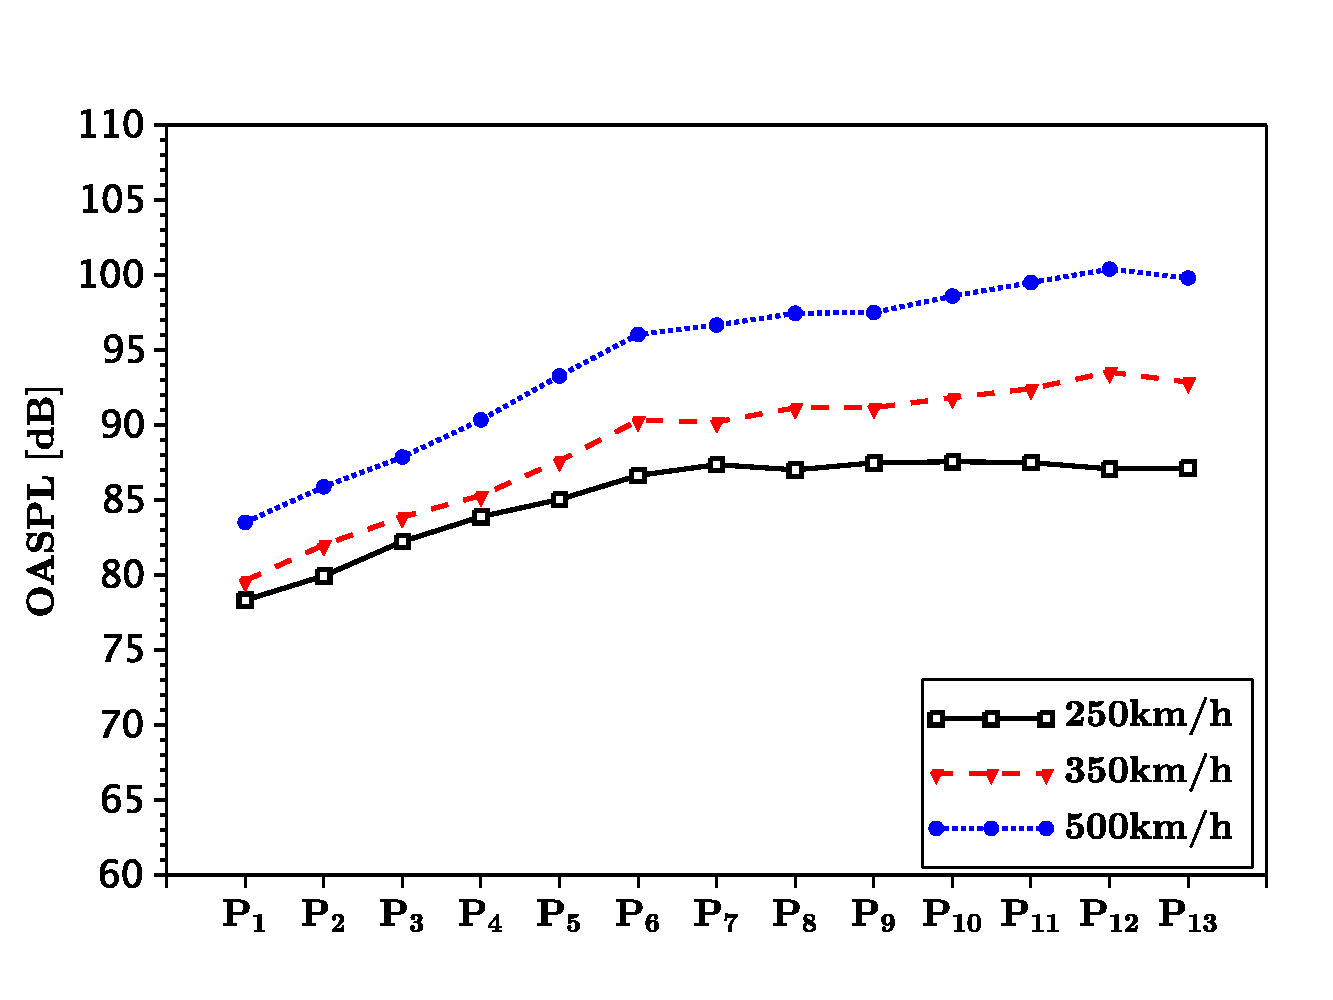
\includegraphics[width=0.55\textwidth]{Figures/oaspl_a.pdf}
  \neufigcaption{fig:ch0-cover}{外部图片插入样例}{Example of Including an External Image}
\end{figure}

\neufigref{fig:ch0-cover} 展示了通过 \verb|\includegraphics| 插入图片文件的方式。
正式论文中建议将图片统一放入 \texttt{Figures} 目录，并使用相对路径引用。

\subsection{PDF 或位图图片}
\begin{figure}[!htbp]
  \centering
  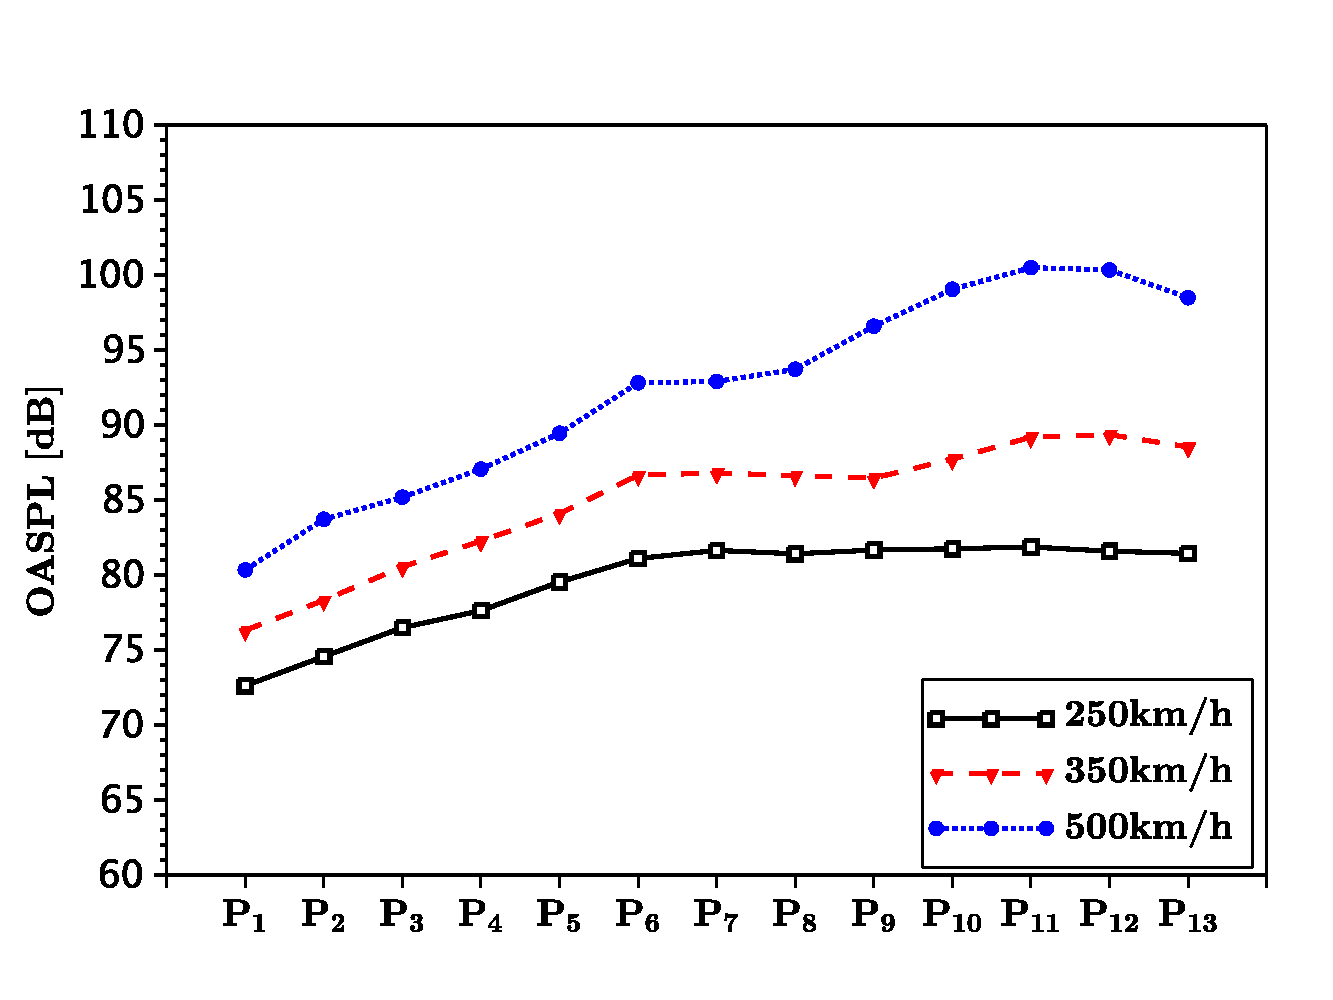
\includegraphics[width=0.55\textwidth]{Figures/oaspl_b.pdf}
  \neufigcaption{fig:ch0-pdf}{PDF 图片插入样例}{Example of Including a PDF Figure}
\end{figure}

PDF、PNG、JPG 等常见图片格式均可通过 \verb|\includegraphics| 插入。
若图片由绘图软件或数据分析程序导出，建议优先使用 PDF 格式以保持较清晰的显示效果。

\subsection{并列图片}
\begin{figure}[!htbp]
  \centering
  \begin{minipage}[t]{0.49\linewidth}
    \centering
    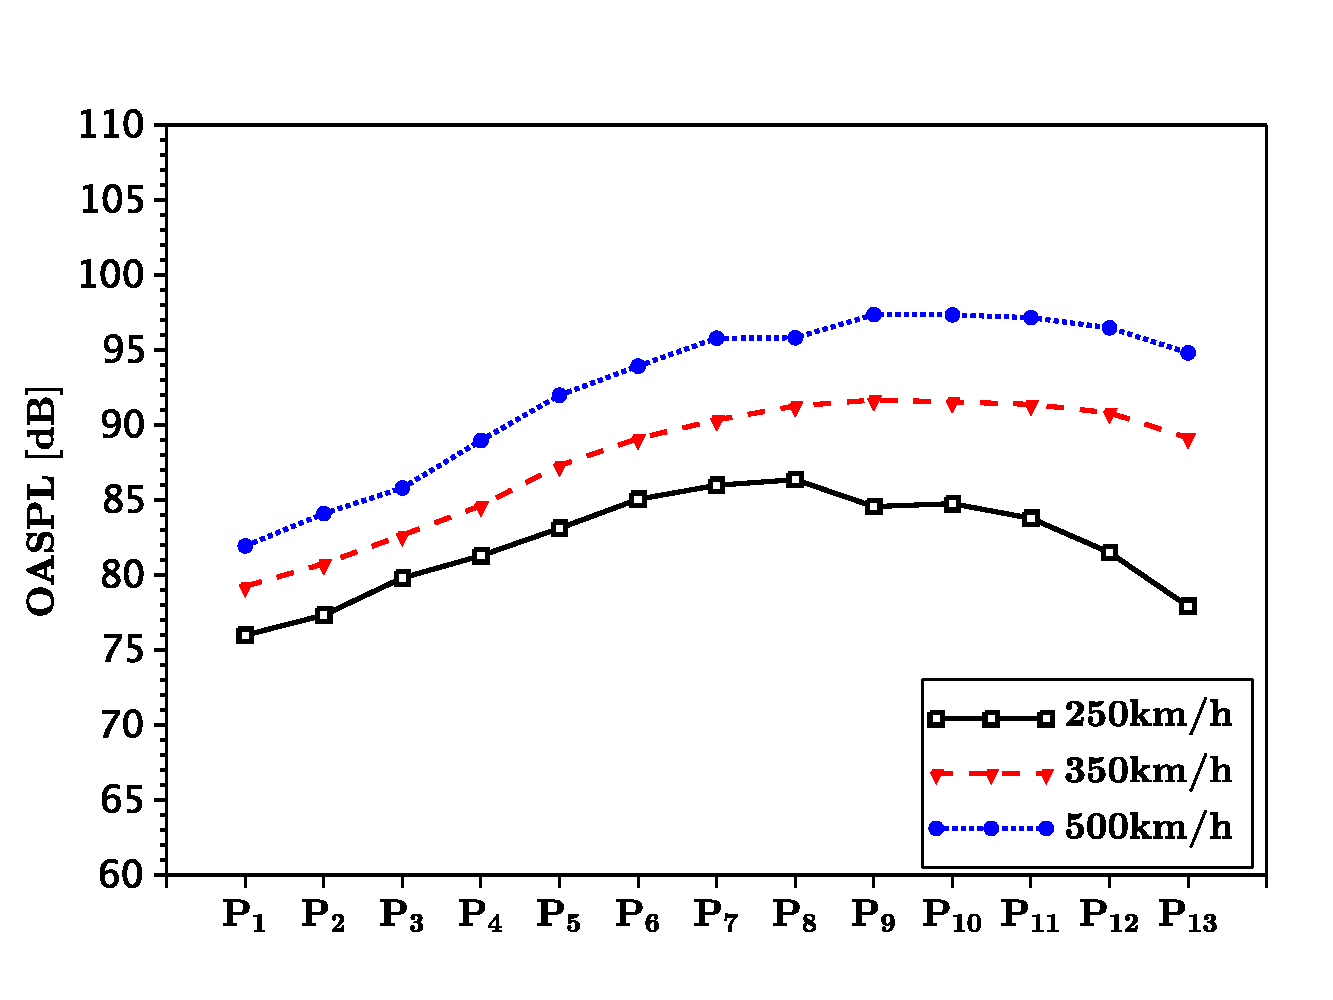
\includegraphics[width=\linewidth]{Figures/oaspl_c.pdf}
  \end{minipage}
  \hfill
  \begin{minipage}[t]{0.49\linewidth}
    \centering
    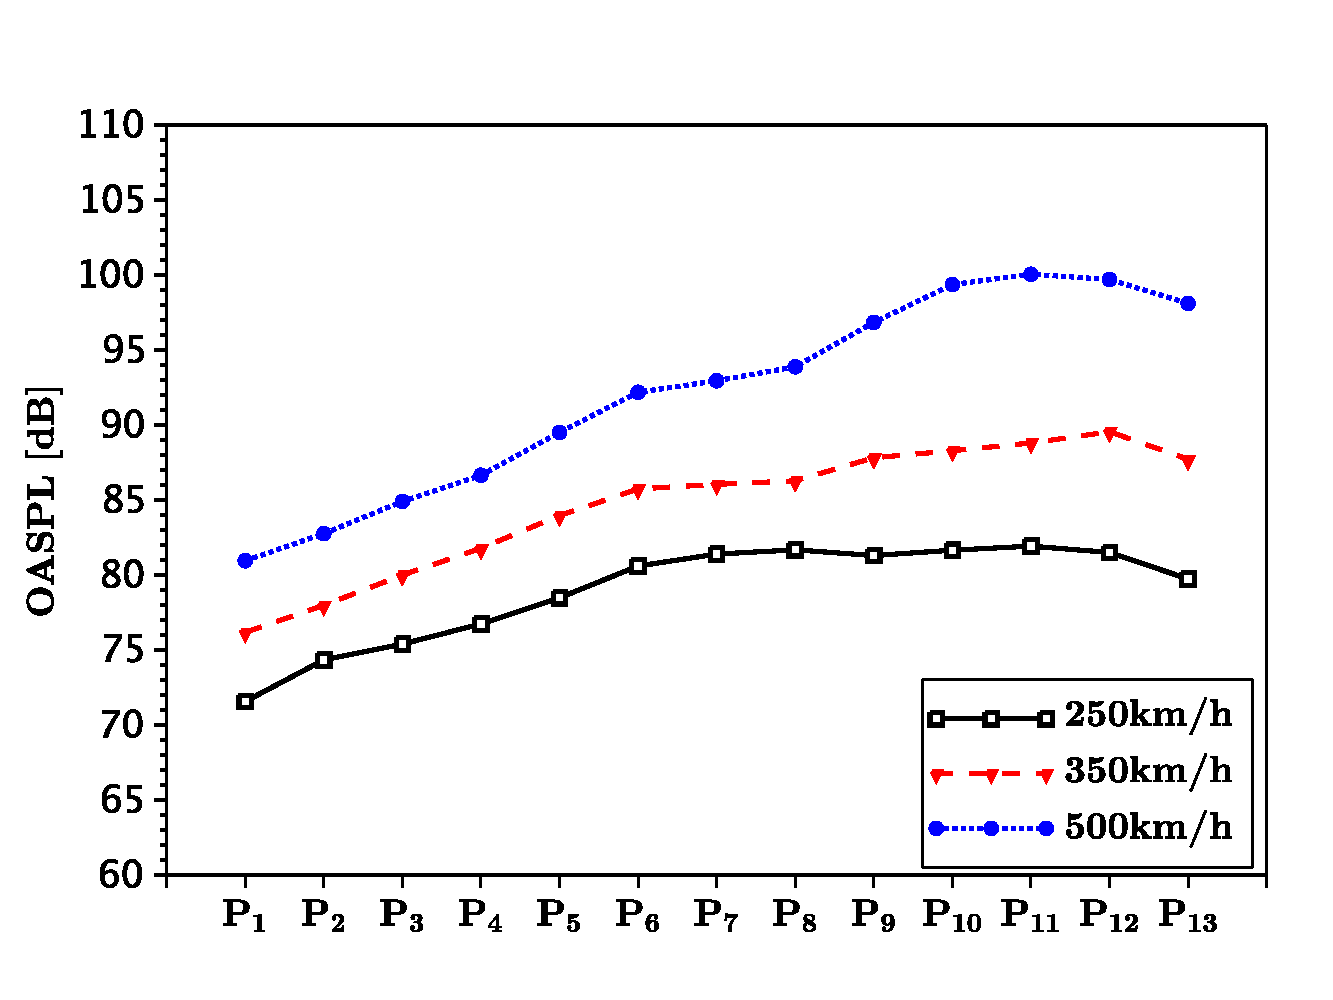
\includegraphics[width=\linewidth]{Figures/oaspl_d.pdf}
  \end{minipage}
  \neufigcaption{fig:ch0-side-by-side}{普通并列图形排版样例}{Example of Side-by-Side Figures}
\end{figure}

\neufigref{fig:ch0-side-by-side} 使用 \texttt{minipage} 完成普通并列排版。
当两幅图共享一个总标题且不需要分别引用时，可使用这种方式。

\subsection{并列子图}
\begin{figure}[!htbp]
  \centering
  \begin{neusubfigure}{0.49\linewidth}
    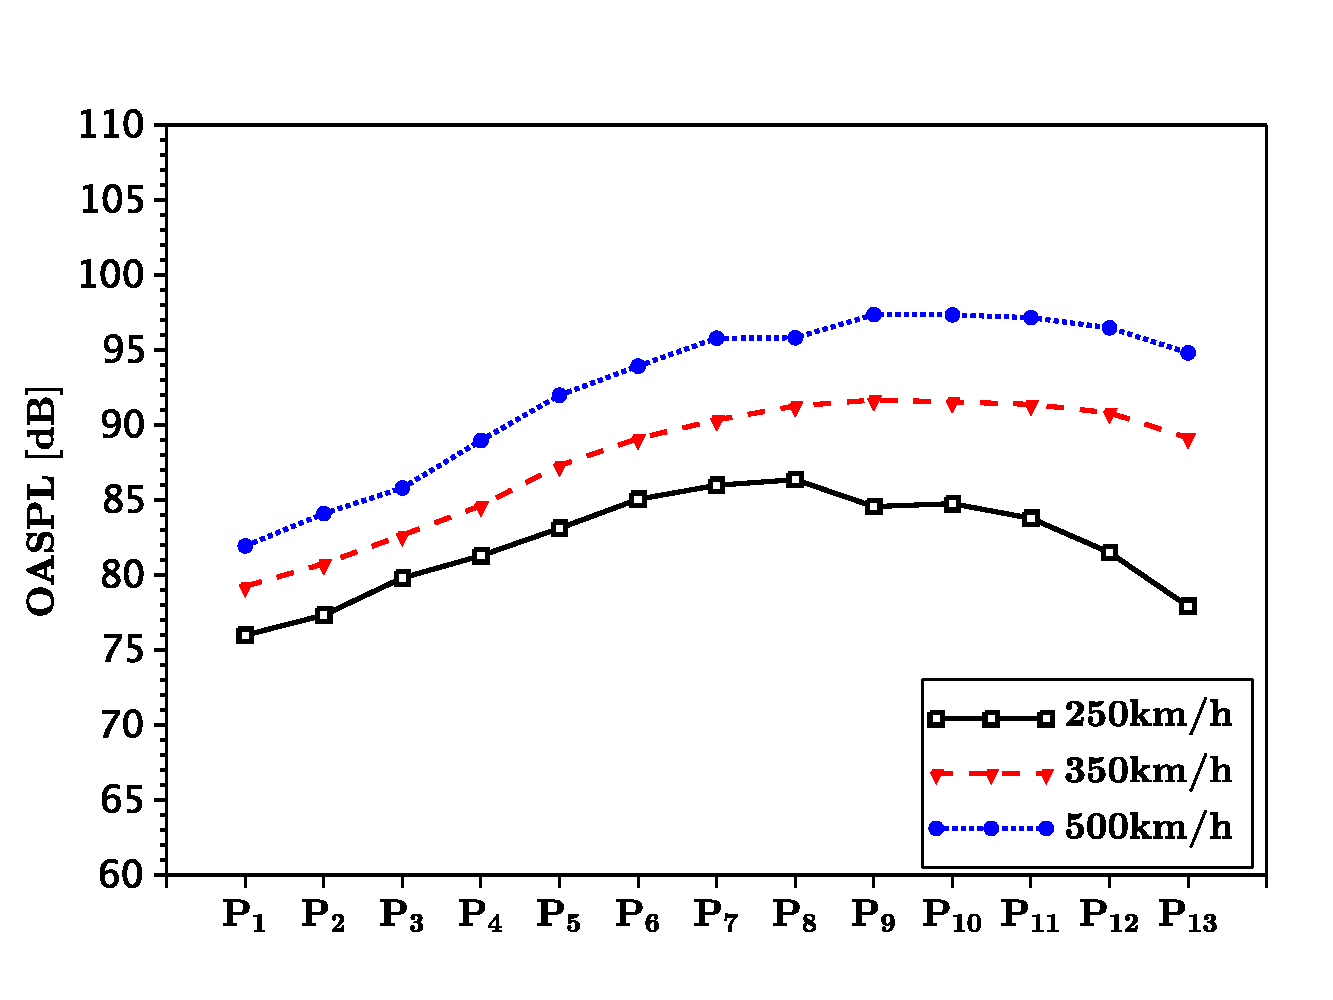
\includegraphics[width=\linewidth]{Figures/oaspl_c.pdf}
    \neusubfigcaption{fig:ch0-side-by-side-a}{工况一}
  \end{neusubfigure}
  \hfill
  \begin{neusubfigure}{0.49\linewidth}
    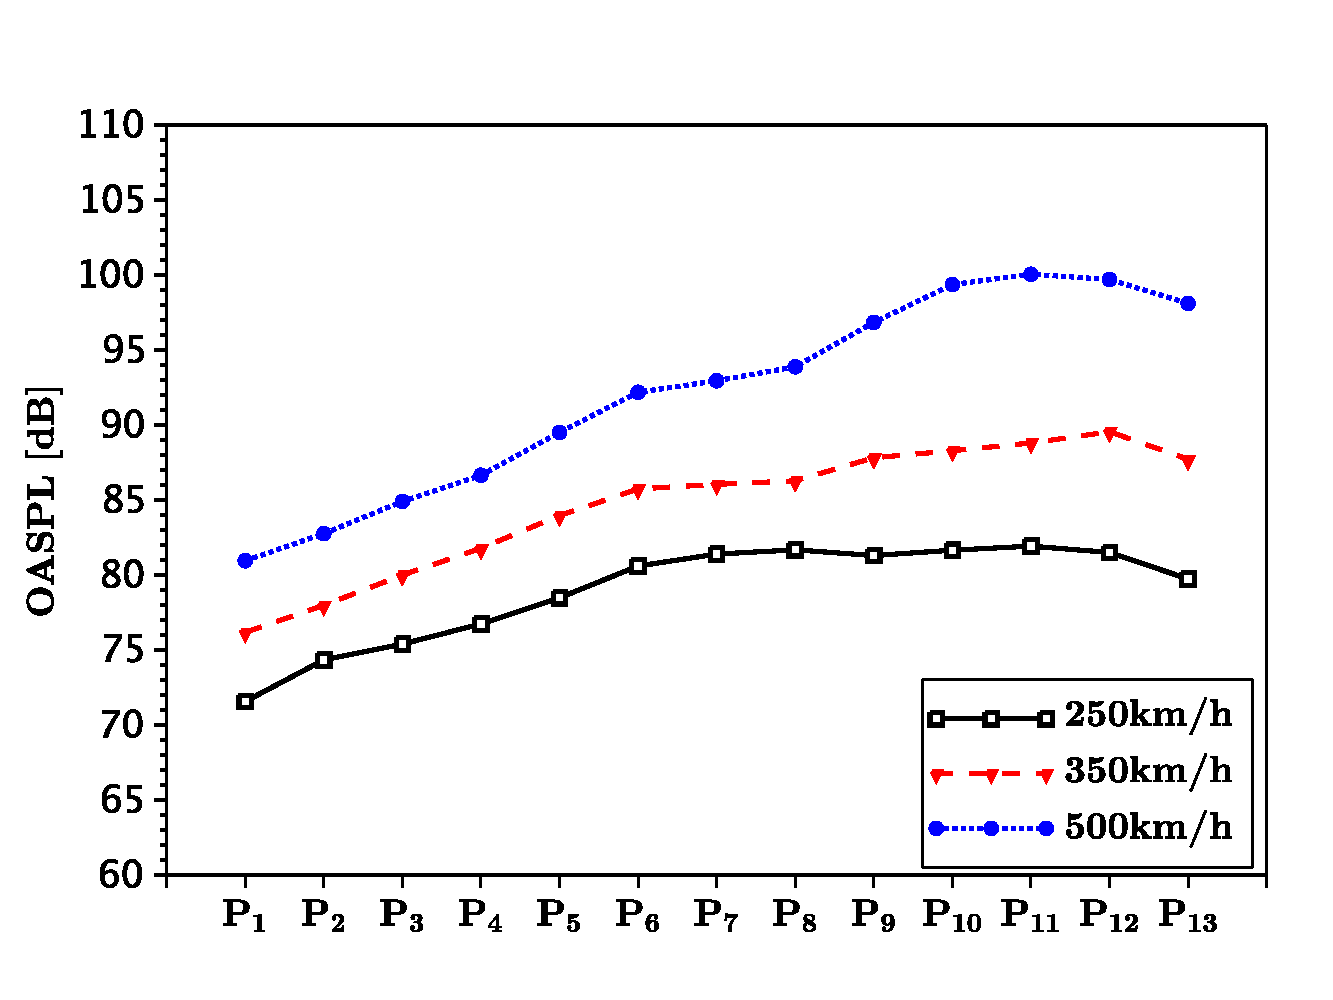
\includegraphics[width=\linewidth]{Figures/oaspl_d.pdf}
    \neusubfigcaption{fig:ch0-side-by-side-b}{工况二}
  \end{neusubfigure}
  \neufigcaption{fig:ch0-subfigures}{并列子图排版样例}{Example of Side-by-Side Subfigures}
\end{figure}

\neufigref{fig:ch0-subfigures} 使用 \texttt{neusubfigure} 完成并列子图排版。
其中 \neusubfigref{fig:ch0-side-by-side-a} 和 \neusubfigref{fig:ch0-side-by-side-b} 可分别引用到子图。
当两幅图共享一个总标题且需要分别引用时，可使用这种方式；如果每幅图需要完全独立的图号，建议拆成两个独立的 \texttt{figure} 环境。

\subsection{二乘二子图}
\begin{figure}[!htbp]
  \centering
  \begin{neusubfigure}{0.49\linewidth}
    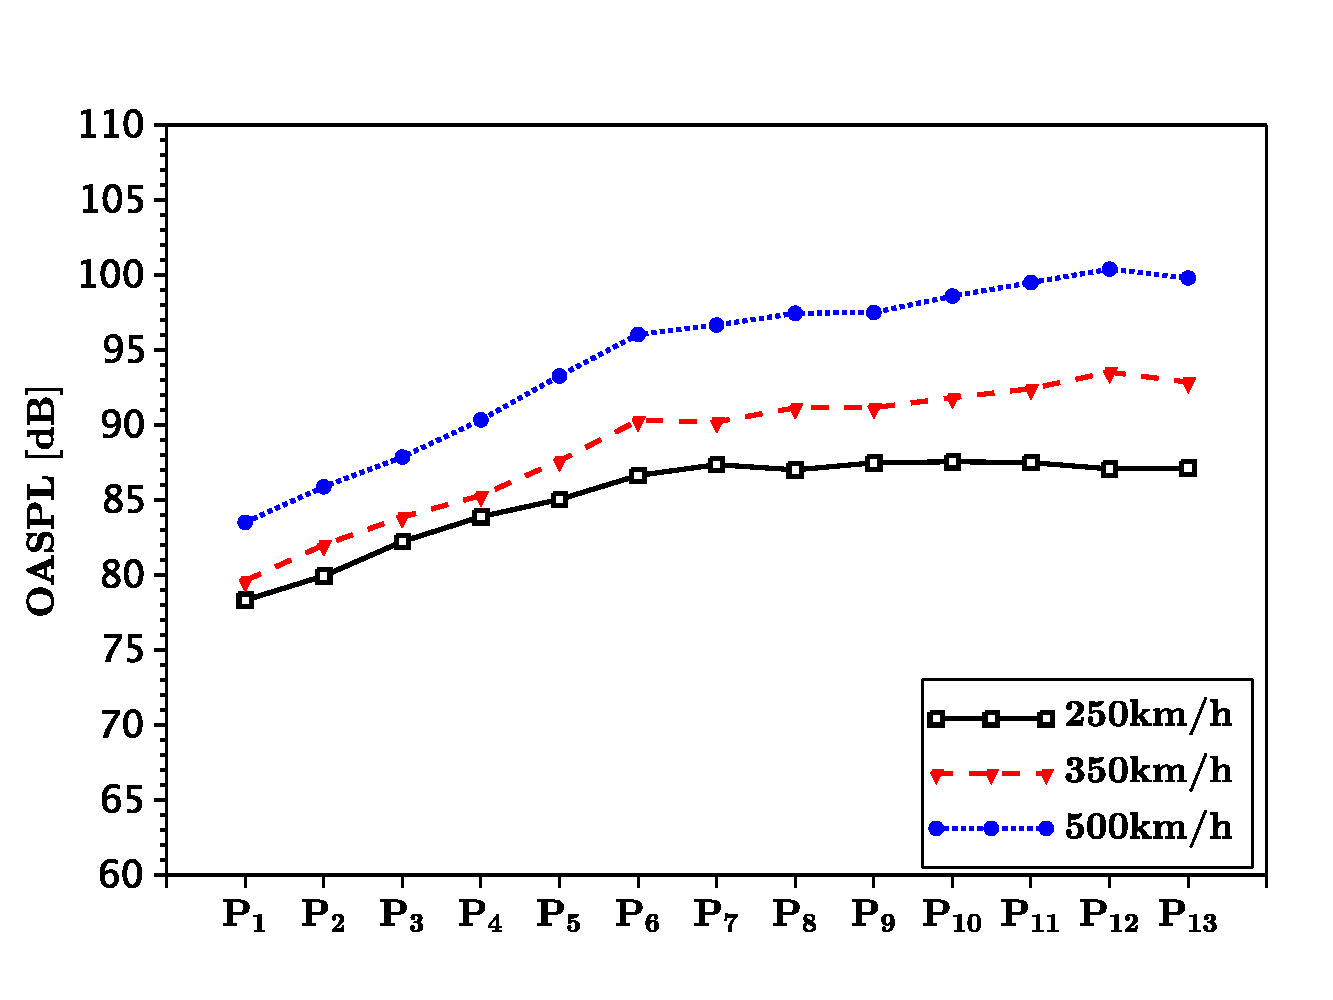
\includegraphics[width=\linewidth]{Figures/oaspl_a.pdf}
    \neusubfigcaption{fig:ch0-four-subfig-a}{工况一}
  \end{neusubfigure}
  \hfill
  \begin{neusubfigure}{0.49\linewidth}
    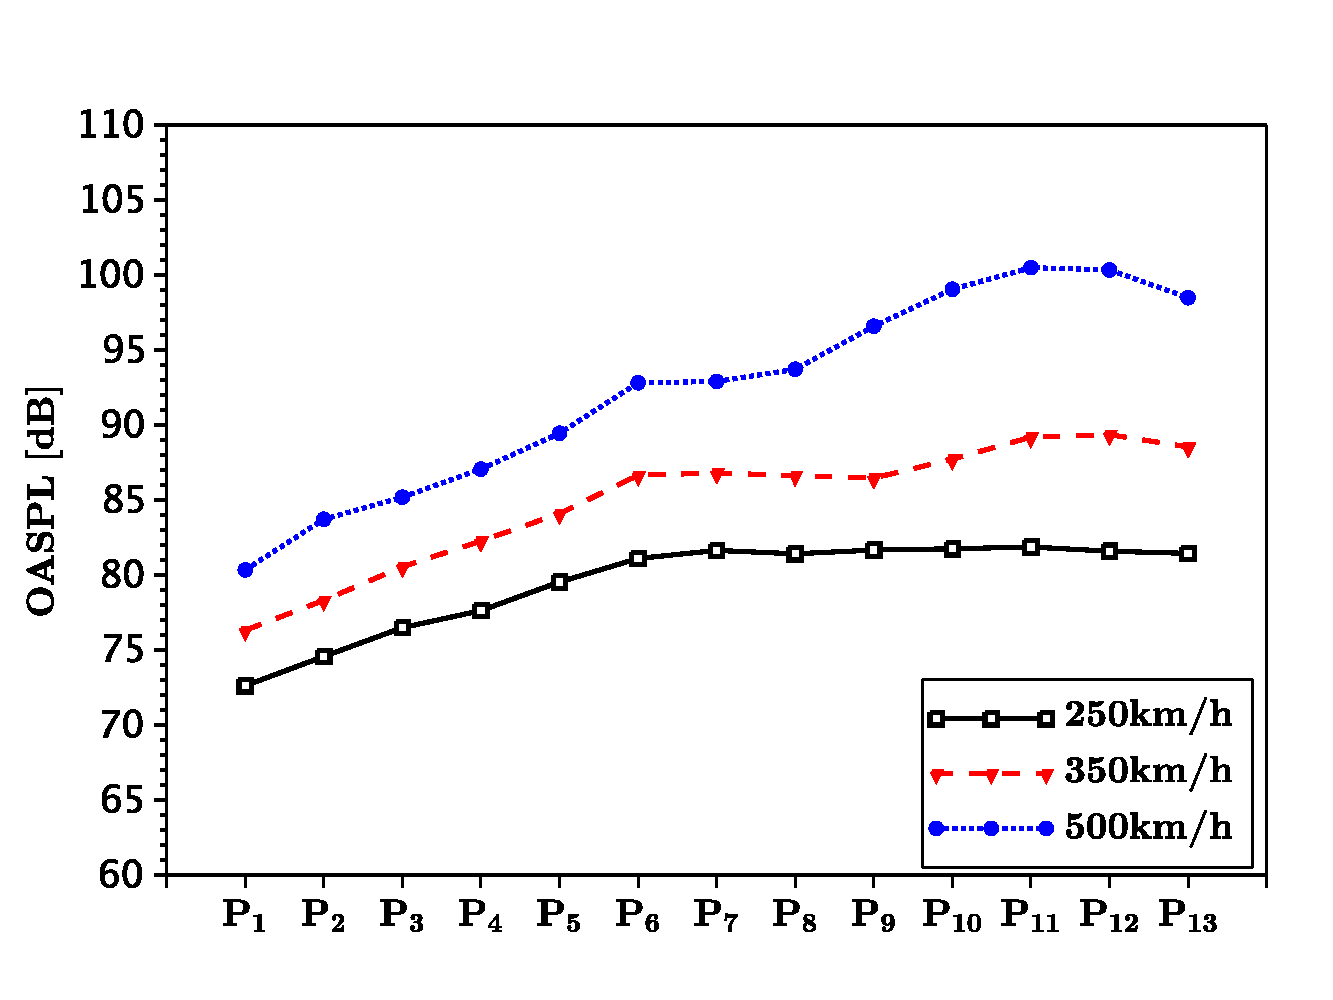
\includegraphics[width=\linewidth]{Figures/oaspl_b.pdf}
    \neusubfigcaption{fig:ch0-four-subfig-b}{工况二}
  \end{neusubfigure}
  \par\vspace{2bp}

  \begin{neusubfigure}{0.49\linewidth}
    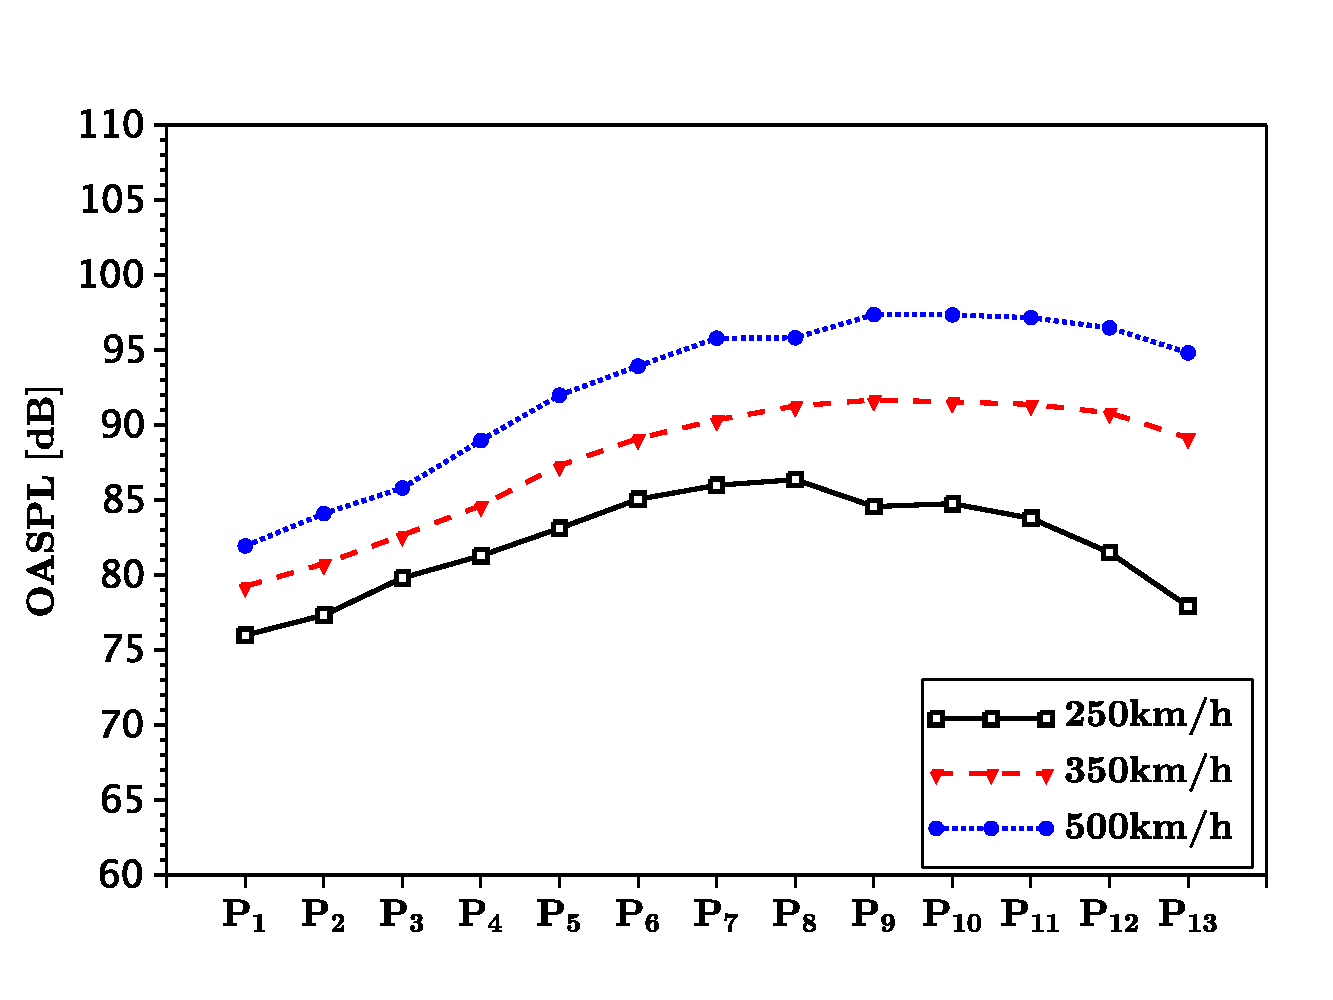
\includegraphics[width=\linewidth]{Figures/oaspl_c.pdf}
    \neusubfigcaption{fig:ch0-four-subfig-c}{工况三}
  \end{neusubfigure}
  \hfill
  \begin{neusubfigure}{0.49\linewidth}
    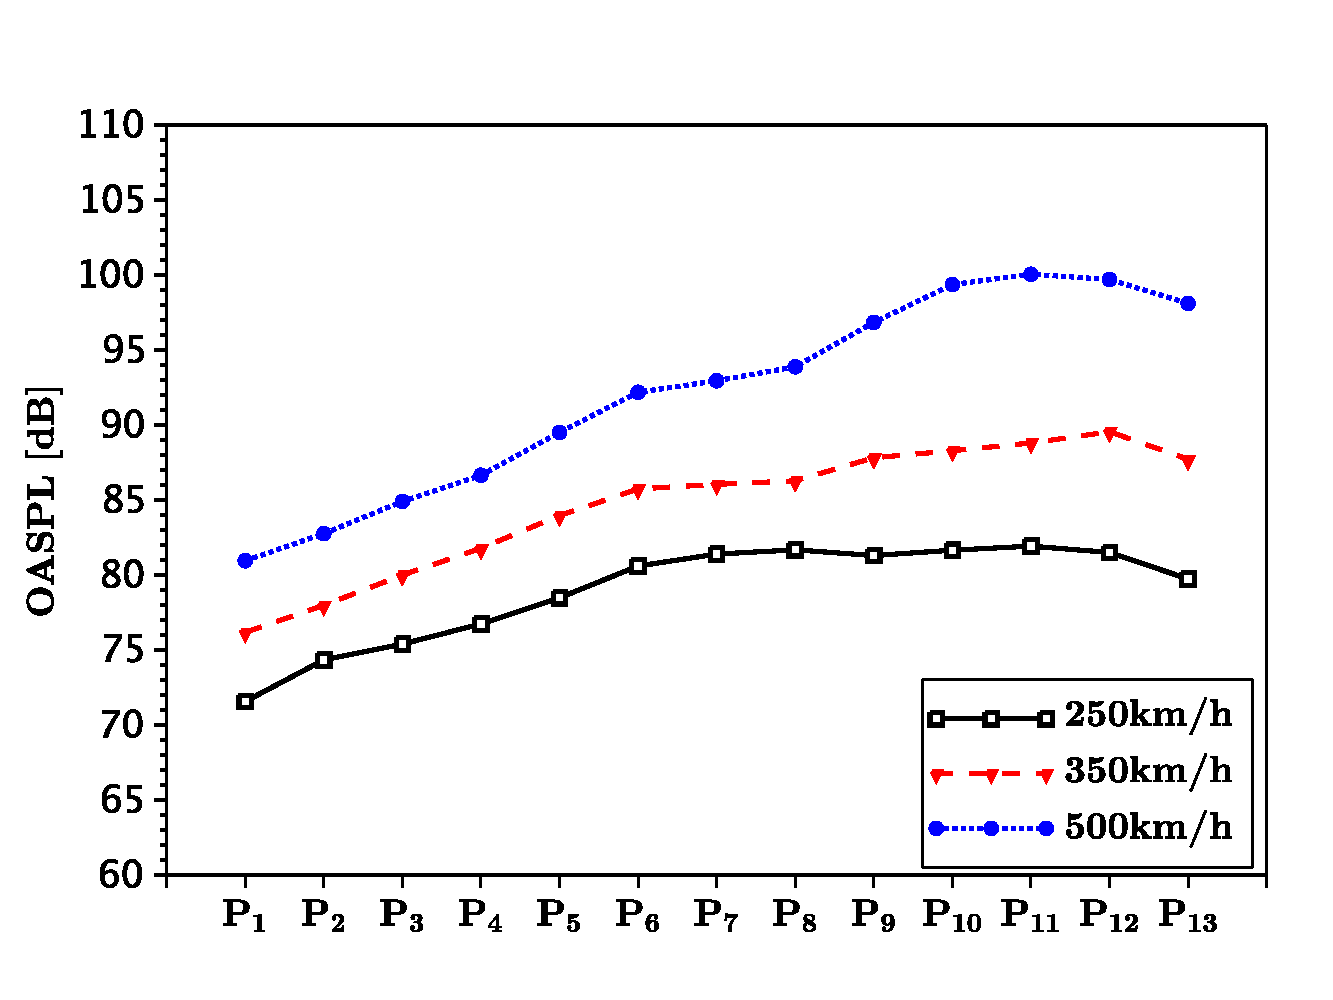
\includegraphics[width=\linewidth]{Figures/oaspl_d.pdf}
    \neusubfigcaption{fig:ch0-four-subfig-d}{工况四}
  \end{neusubfigure}
  \neufigcaption{fig:ch0-four-subfigures}{二乘二子图排版样例}{Example of Two-by-Two Subfigures}
\end{figure}

\neufigref{fig:ch0-four-subfigures} 展示了四幅子图的二乘二排布。
例如 \neusubfigref{fig:ch0-four-subfig-a} 至 \neusubfigref{fig:ch0-four-subfig-d} 可分别引用到四个子图。
排版时建议注意以下几点：
\begin{itemize}
  \item 子图宽度通常可取 \verb|0.48\linewidth| 至 \verb|0.49\linewidth|。
  \item 每行两个子图之间使用 \verb|\hfill| 自动拉开横向间距。
  \item 两行之间可用少量 \verb|\par\vspace| 控制垂直间距。
\end{itemize}

\section{表格排版}

本模板提供 \verb|\neutabcaption{label}{中文题名}{English title}| 用于生成中英文表题。
表题应置于表格上方，正文中使用 \verb|\neutabref{label}| 引用。
表格同样建议使用 \verb|[!htbp]|。如果表格过高导致页底空白，优先考虑缩小字号、调整列宽、拆分表格或使用跨页表格，而不是强制分页。

\subsection{三线表}

\begin{table}[!htbp]
  \centering
  \neutabcaption{tab:ch0-booktabs}{三线表样例}{Example of a Three-Line Table}
  \begin{tabular}{lccc}
    \toprule
    方法       & 准确率（\%）       & 召回率（\%）       & F1 值           \\
    \midrule
    Baseline & 85.2          & 84.1          & 0.846          \\
    Method A & 89.7          & 88.9          & 0.893          \\
    Proposed & \textbf{92.1} & \textbf{91.5} & \textbf{0.918} \\
    \bottomrule
  \end{tabular}
\end{table}

\neutabref{tab:ch0-booktabs} 展示了推荐的三线表格式。
论文中应尽量避免过多竖线，以保持表格简洁。

\subsection{复杂表格}
\begin{table}[!htbp]
  \centering
  \neutabcaption{tab:ch0-complex}{合并单元格与自动换行表格样例}{Example of Merged Cells and Auto-Wrapping Columns}
  \begin{tabularx}{\textwidth}{llXc}
    \toprule
    类别                  & 指标  & 说明                               & 是否必需 \\
    \midrule
    \multirow{2}{*}{图形} & 分辨率 & 位图图片应保证在最终 PDF 中清晰可辨。            & 是    \\
                        & 题名  & 图题使用中英文双语标题，并位于图片下方。             & 是    \\
    \midrule
    \multirow{2}{*}{表格} & 宽度  & 宽表格可使用 \texttt{tabularx} 自动分配列宽。 & 否    \\
                        & 表注  & 表内说明应简明，必要时可在正文中解释。              & 否    \\
    \bottomrule
  \end{tabularx}
\end{table}

\neutabref{tab:ch0-complex} 同时展示了 \verb|\multirow|、\verb|\makecell| 可配合使用的复杂表格场景。
若单元格内容较长，优先使用 \texttt{tabularx} 或 \texttt{p\{...\}} 列类型控制宽度。

\section{公式排版}

公式应使用标准数学环境，并通过 \verb|\label| 设置标签。
引用公式时建议使用模板提供的 \verb|\neueqref{label}|。

\subsection{单行公式}
以分类任务中的交叉熵损失为例，可写为
\begin{equation}
  \mathcal{L}(\theta)
  = - \frac{1}{N}\sum_{i=1}^{N}\sum_{k=1}^{K} y_{ik}\log p_{ik}
  \label{eq:ch0-loss}
\end{equation}

如 \neueqref{eq:ch0-loss} 所示，带编号公式适合放置正文中需要引用的重要定义。

\subsection{多行公式}
循环模型中的状态更新和输出计算可写为
\begin{align}
  h_t       & = \sigma(W_x x_t + W_h h_{t-1} + b), \label{eq:ch0-state} \\
  \hat{y}_t & = \operatorname{softmax}(W_o h_t). \label{eq:ch0-output}
\end{align}

\neueqref{eq:ch0-state} 和 \neueqref{eq:ch0-output} 展示了多行公式的编号方式。
如果多行推导只需要一个编号，可使用 \texttt{aligned} 放在 \texttt{equation} 环境内部。

\subsection{分段函数与矩阵}
分段函数和矩阵经常同时出现在数学定义中，例如
\begin{equation}
  g(x)=
  \begin{cases}
    0, & x < 0,       \\
    x, & 0 \le x < 1, \\
    1, & x \ge 1,
  \end{cases}
  \qquad
  A =
  \begin{bmatrix}
    1 & 0 & 0 \\
    0 & 1 & 0 \\
    0 & 0 & 1
  \end{bmatrix}.
  \label{eq:ch0-piecewise}
\end{equation}

\neueqref{eq:ch0-piecewise} 展示了分段函数和矩阵的常见写法。

\section{算法伪代码}

计算机类论文常需要给出算法步骤。本文档在 \texttt{main.tex} 中加载了 \texttt{algorithm} 和 \texttt{algorithmic} 宏包，可以直接使用如下环境。

\begin{algorithm}[!htbp]
  \caption{样例训练流程}
  \label{alg:ch0-training}
  \begin{algorithmic}[1]
    \REQUIRE Training set $\mathcal{D}$, learning rate $\eta$, maximum epoch $T$
    \ENSURE Model parameters $\theta$
    \STATE Initialize parameters $\theta$
    \FOR{$t = 1$ to $T$}
    \STATE Sample a mini-batch $\mathcal{B}$ from $\mathcal{D}$
    \STATE Compute loss $\mathcal{L}(\theta)$ by \neueqref{eq:ch0-loss}
    \STATE Update $\theta \leftarrow \theta - \eta \nabla_{\theta}\mathcal{L}(\theta)$
    \ENDFOR
    \RETURN $\theta$
  \end{algorithmic}
\end{algorithm}

算法~\ref{alg:ch0-training} 展示了带行号的伪代码。
若需要中文关键字，可在导言区重定义相应命令。

\section{引用、链接与交叉引用}

参考文献引用可使用两种模板命令：
\begin{itemize}
  \item 上标引用使用 \verb|\upcite{key}|，适合放在句末，例如已有研究讨论了神经网络轻量化问题\upcite{guo_2023_research}。
  \item 正文引用使用 \verb|\inlinecite{key}|，适合作为句子成分，例如文献 \inlinecite{thakkar_2018_performance} 给出了系统性能评测案例。
\end{itemize}
多篇文献可写在同一条引用命令中，例如区块链平台相关研究\upcite{zheng_2019_nutbaas,thakkar_2018_performance}。

交叉引用建议统一使用模板命令：
\begin{itemize}
  \item 图引用：\verb|\neufigref{fig:ch0-pdf}|，效果为 \neufigref{fig:ch0-pdf}。
  \item 子图引用：\verb|\neusubfigref{fig:ch0-four-subfig-a}|，效果为 \neusubfigref{fig:ch0-four-subfig-a}。
  \item 表引用：\verb|\neutabref{tab:ch0-complex}|，效果为 \neutabref{tab:ch0-complex}。
  \item 公式引用：\verb|\neueqref{eq:ch0-loss}|，效果为 \neueqref{eq:ch0-loss}。
  \item 算法引用：当前模板未单独封装算法引用命令，可写作“算法~\ref{alg:ch0-training}”。
\end{itemize}
模板提供的公开命令和环境可参考 \texttt{README.md} 中的“模板命令说明”一节。
|，并从第~\ref{chap:introduction}~章开始组织正式内容。

\section{章节层级与正文段落}

论文正文通常从一级标题开始组织内容，一级标题使用 \verb|\chapter|，二级标题使用 \verb|\section|，三级标题使用 \verb|\subsection|。
本模板会自动设置章标题、节标题、页眉、页码和目录格式，作者只需要关注正文内容。
正文段落首行缩进、行距和中英文字体均由模板统一控制，一般不需要在正文中手动设置字号、字体或段间距。

中文正文可以直接书写；英文术语建议在首次出现时给出全称，例如自然语言处理（Natural Language Processing, NLP）。
行内公式可以写作 $E=mc^2$，行内代码或命令可以使用 \verb|\verb|，例如 \verb|%!TEX root = ./main.tex
\chapter{论文格式样例与模板验证}

本章作为模板的集中样例章，用于快速检查正文中常见排版元素的显示效果。
样例覆盖章节层级、正文段落、列表、脚注、图、表、公式、算法、交叉引用和参考文献引用等内容。
编写正式论文时，可以保留本章作为排版对照；定稿前可在 \texttt{main.tex} 中删除或注释 \verb|\input{chapter0-guide}|，并从第~\ref{chap:introduction}~章开始组织正式内容。

\section{章节层级与正文段落}

论文正文通常从一级标题开始组织内容，一级标题使用 \verb|\chapter|，二级标题使用 \verb|\section|，三级标题使用 \verb|\subsection|。
本模板会自动设置章标题、节标题、页眉、页码和目录格式，作者只需要关注正文内容。
正文段落首行缩进、行距和中英文字体均由模板统一控制，一般不需要在正文中手动设置字号、字体或段间距。

中文正文可以直接书写；英文术语建议在首次出现时给出全称，例如自然语言处理（Natural Language Processing, NLP）。
行内公式可以写作 $E=mc^2$，行内代码或命令可以使用 \verb|\verb|，例如 \verb|\input{chapter0-guide}|。
脚注示例如此处所示\footnote{脚注用于补充说明，不宜放置过长的正文内容。}。
若某页因图表浮动或分页规则没有排满，脚注可能跟随正文排版区而显得略高，这是正常的 LaTeX 页面构建结果。

\subsection{字体、字号与强调}

模板预定义了常用中文字体命令。正式论文中通常不需要手动切换字体；只有在展示样式、术语强调或特殊说明时才建议使用。
当前模板已经为默认宋体和 \verb|\song| 字族配置伪粗体，因此 \verb|\textbf| 或 \verb|\bfseries| 可以用于中文局部强调。
需要注意的是，中文加粗应克制使用；标题层级、术语定义或表格重点值可以适当加粗，大段正文不建议整体加粗。
如果需要更明显的标题式强调，可使用黑体或调整标题层级；如果只是普通正文重点，优先使用 \verb|\textbf|。

\begin{table}[!htbp]
  \centering
  \neutabcaption{tab:ch0-fonts}{字体与强调样例}{Examples of Fonts and Emphasis}
  \begin{tabular}{lll}
    \toprule
    命令             & 显示效果                         & 使用建议       \\
    \midrule
    \verb|\song|   & {\song 宋体文字示例}               & 正文默认字体     \\
    \verb|\textbf| & \textbf{加粗文字示例}              & 局部强调、表格重点值 \\
    \verb|\hei|    & {\hei 黑体文字示例}                & 标题或较强强调场景  \\
    \verb|\kai|    & {\kai 楷体文字示例}                & 摘要、题签或引用语  \\
    \verb|\fs|     & {\fs 仿宋文字示例}                 & 特殊文书类内容    \\
    \verb|\textit| & \textit{Italic text example} & 英文斜体或变量说明  \\
    \bottomrule
  \end{tabular}
\end{table}

\subsection{列表环境}

无序列表适合列出并列事项：
\begin{itemize}
  \item 图题位于图下方，表题位于表上方。
  \item 图表应使用中英文双语标题。
  \item 公式、图、表、算法均应使用标签进行交叉引用。
\end{itemize}

有序列表适合描述步骤：
\begin{enumerate}
  \item 在 \texttt{main.tex} 中填写论文元信息。
  \item 在各章文件中撰写正文内容。
  \item 使用 \texttt{latexmk -xelatex main.tex} 完成编译。
\end{enumerate}

\section{图形排版}

本模板提供 \verb|\neufigcaption{label}{中文题名}{English title}| 用于生成中英文图题。
图题应置于图形下方，正文中使用 \verb|\neufigref{label}| 引用。
图形建议使用 \verb|[!htbp]| 浮动参数，让 LaTeX 在当前位置、页顶、页底或浮动页中选择较合适的位置；除非必须固定位置，否则不建议使用 \verb|[H]|。

\subsection{外部图片}
\begin{figure}[!htbp]
  \centering
  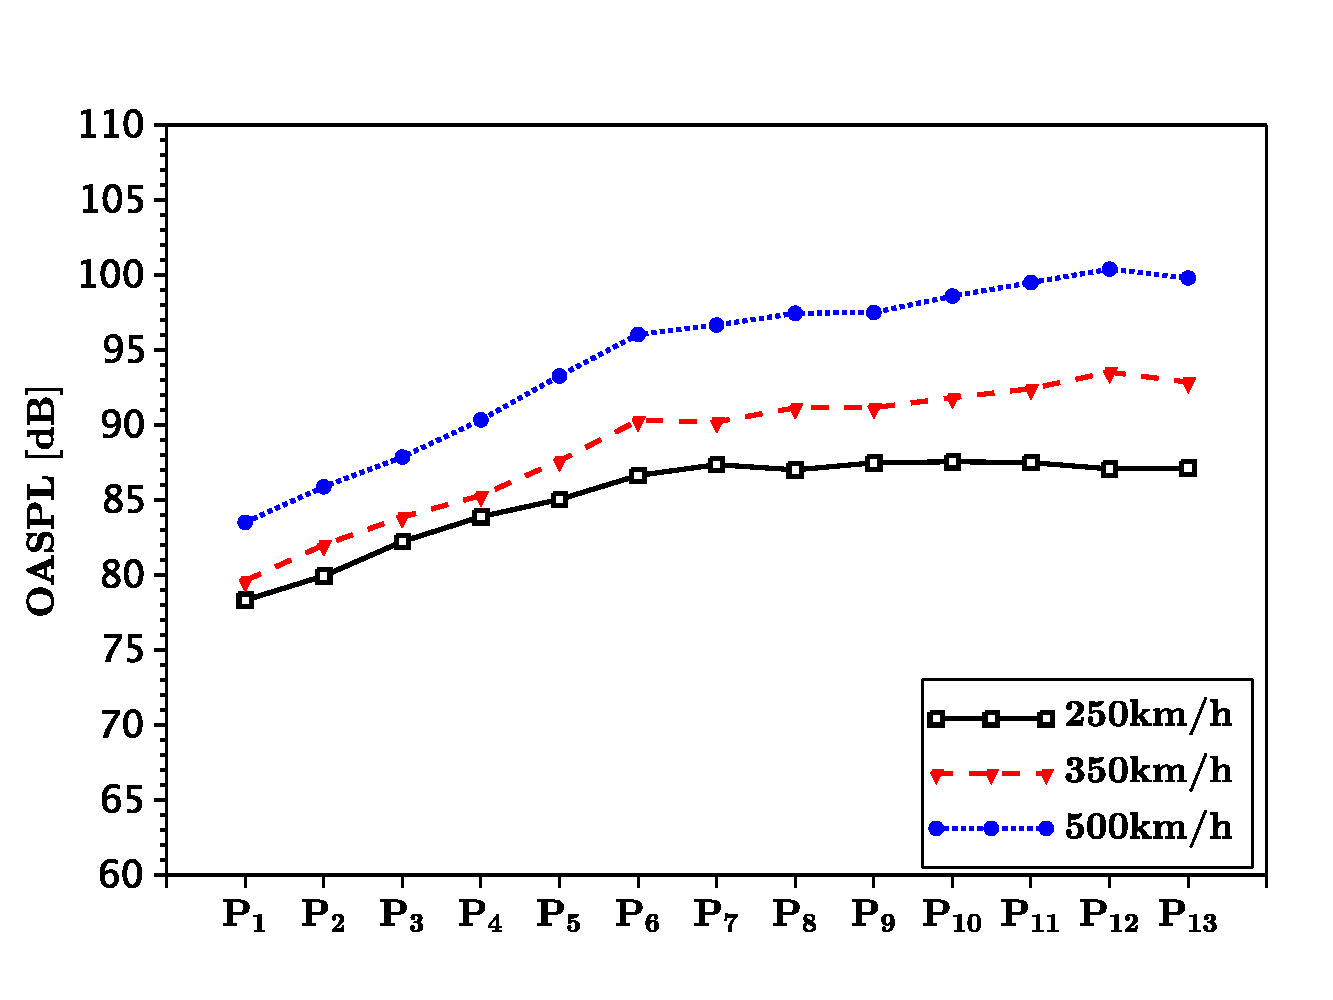
\includegraphics[width=0.55\textwidth]{Figures/oaspl_a.pdf}
  \neufigcaption{fig:ch0-cover}{外部图片插入样例}{Example of Including an External Image}
\end{figure}

\neufigref{fig:ch0-cover} 展示了通过 \verb|\includegraphics| 插入图片文件的方式。
正式论文中建议将图片统一放入 \texttt{Figures} 目录，并使用相对路径引用。

\subsection{PDF 或位图图片}
\begin{figure}[!htbp]
  \centering
  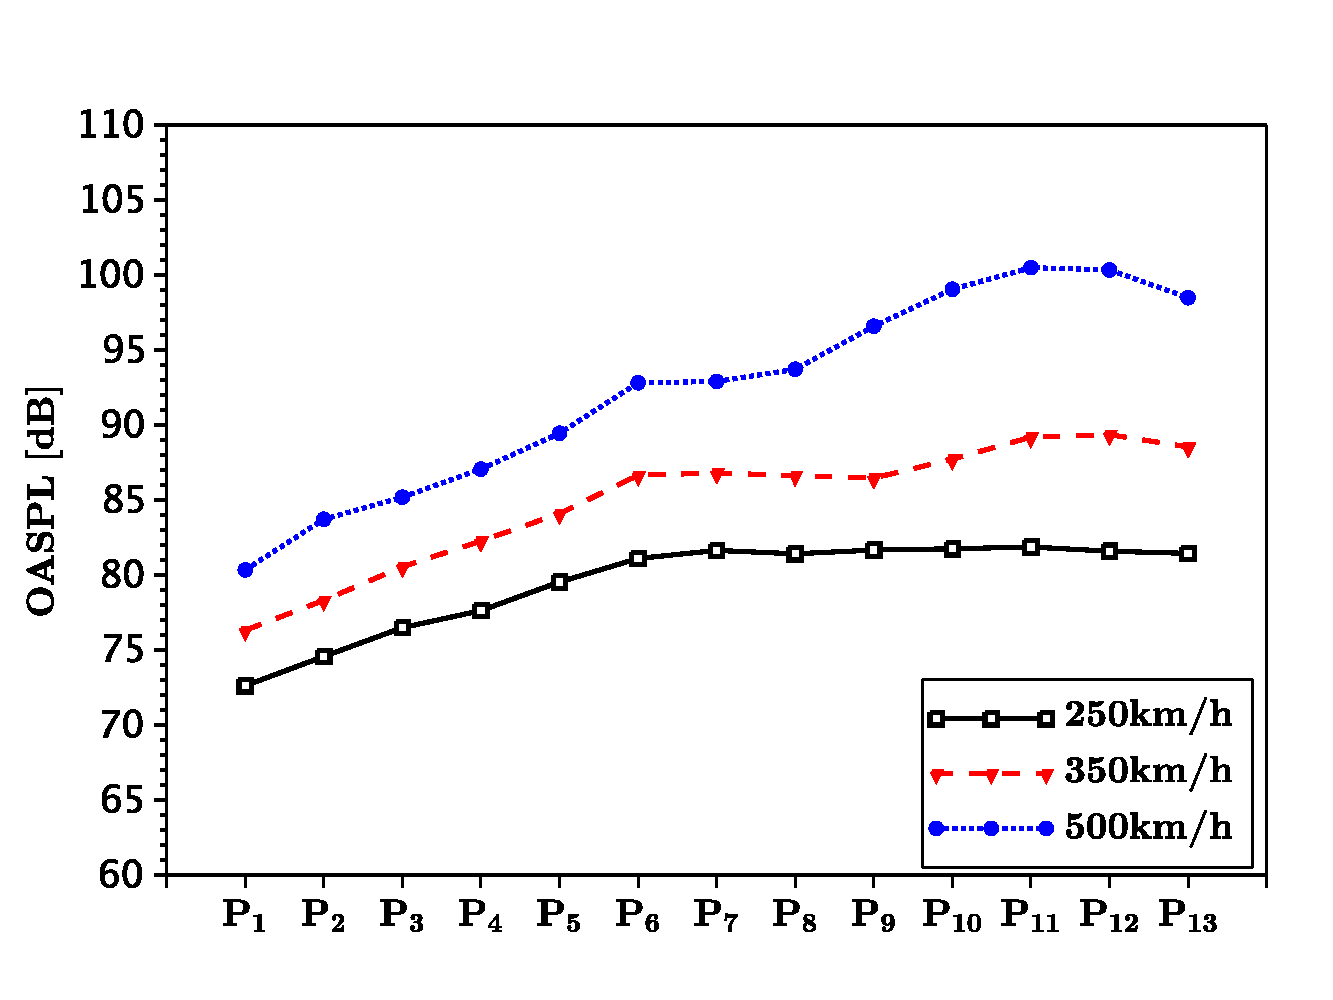
\includegraphics[width=0.55\textwidth]{Figures/oaspl_b.pdf}
  \neufigcaption{fig:ch0-pdf}{PDF 图片插入样例}{Example of Including a PDF Figure}
\end{figure}

PDF、PNG、JPG 等常见图片格式均可通过 \verb|\includegraphics| 插入。
若图片由绘图软件或数据分析程序导出，建议优先使用 PDF 格式以保持较清晰的显示效果。

\subsection{并列图片}
\begin{figure}[!htbp]
  \centering
  \begin{minipage}[t]{0.49\linewidth}
    \centering
    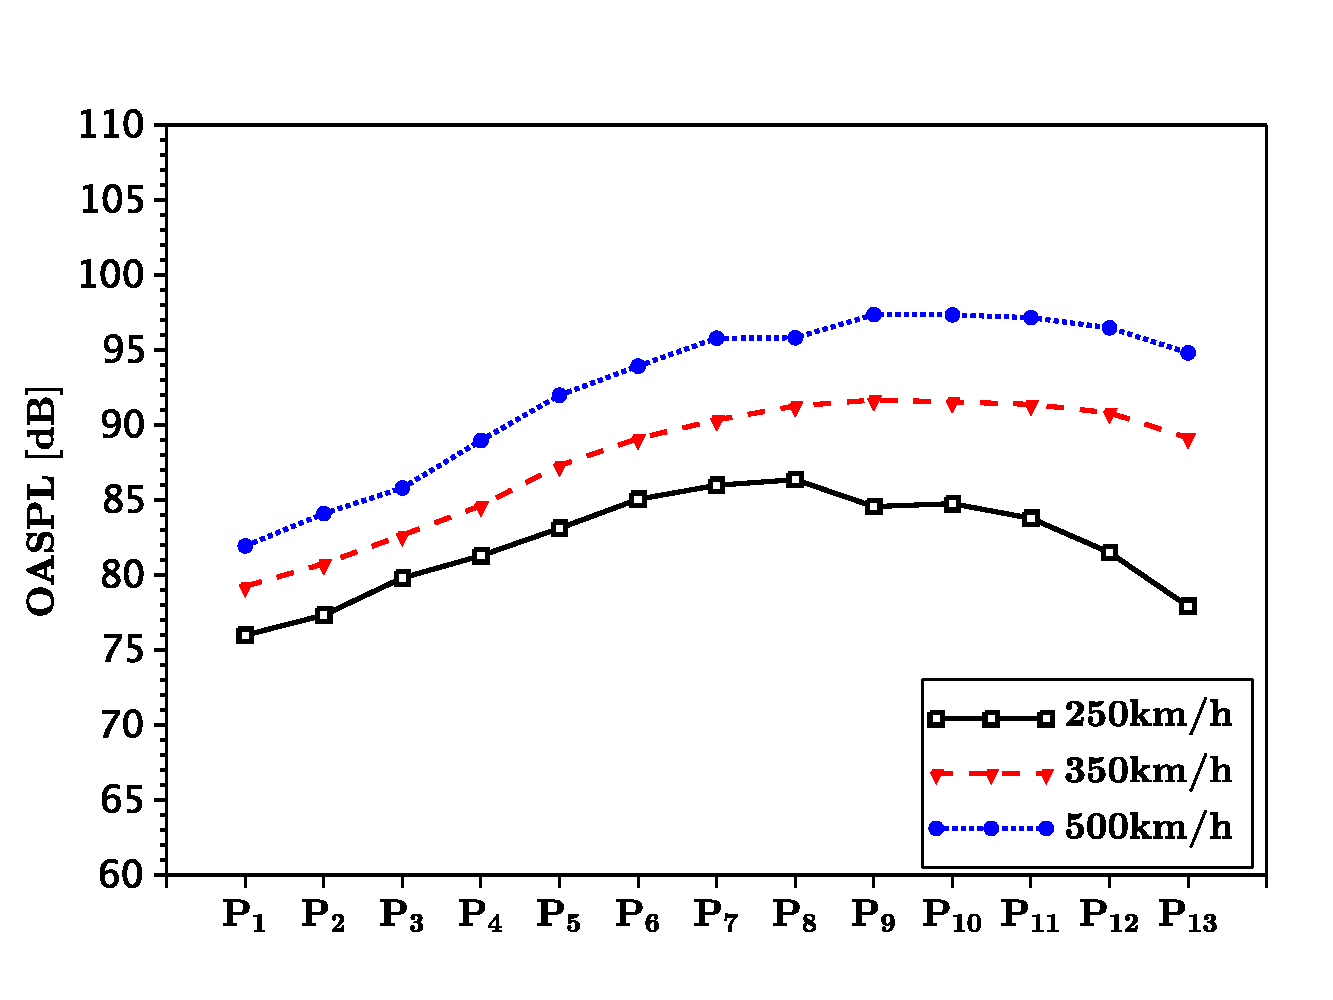
\includegraphics[width=\linewidth]{Figures/oaspl_c.pdf}
  \end{minipage}
  \hfill
  \begin{minipage}[t]{0.49\linewidth}
    \centering
    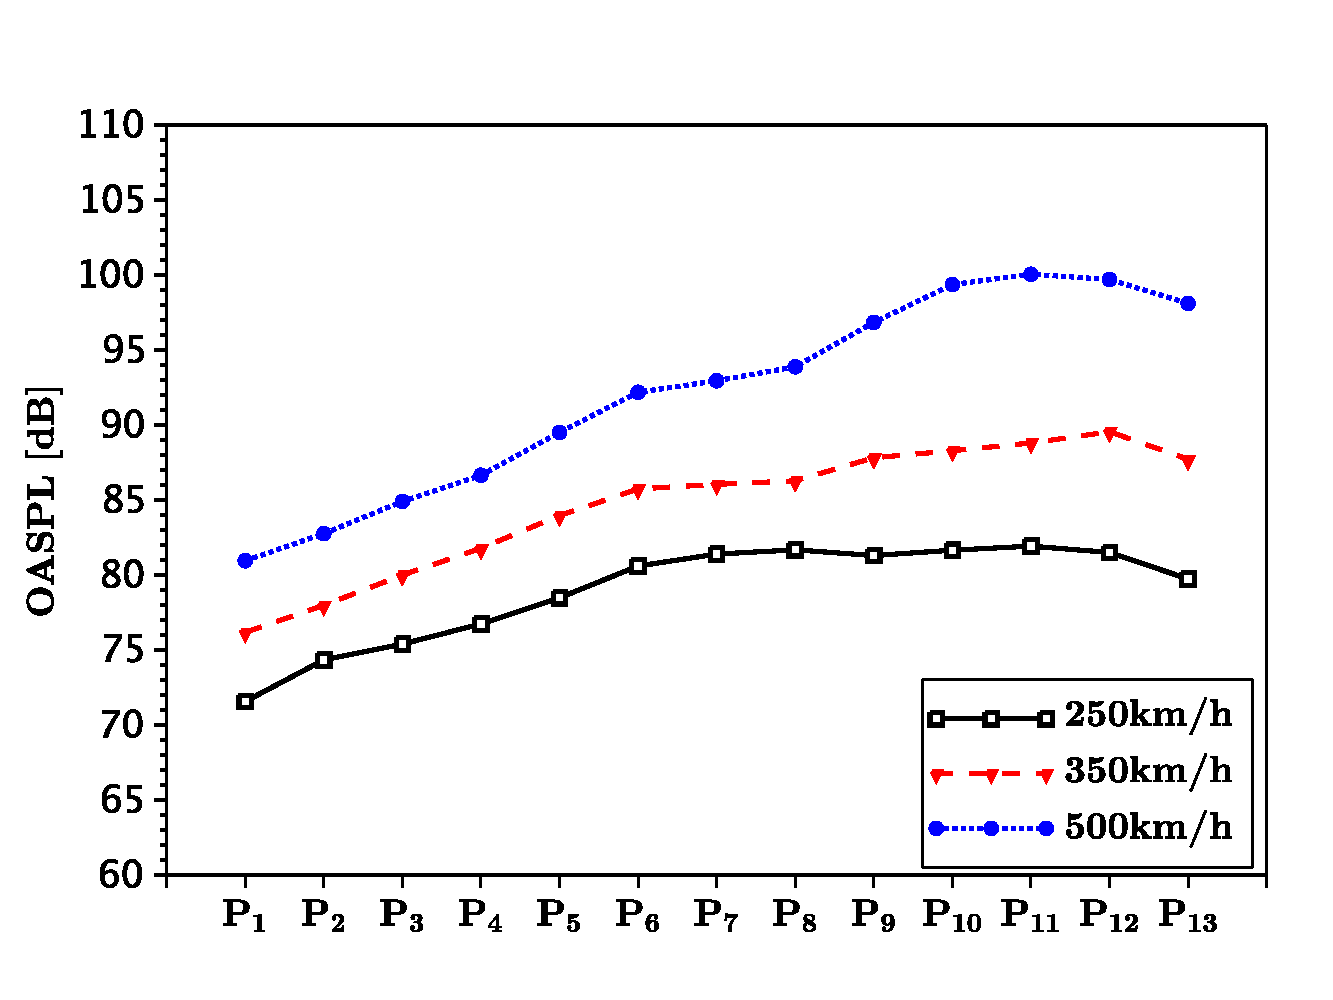
\includegraphics[width=\linewidth]{Figures/oaspl_d.pdf}
  \end{minipage}
  \neufigcaption{fig:ch0-side-by-side}{普通并列图形排版样例}{Example of Side-by-Side Figures}
\end{figure}

\neufigref{fig:ch0-side-by-side} 使用 \texttt{minipage} 完成普通并列排版。
当两幅图共享一个总标题且不需要分别引用时，可使用这种方式。

\subsection{并列子图}
\begin{figure}[!htbp]
  \centering
  \begin{neusubfigure}{0.49\linewidth}
    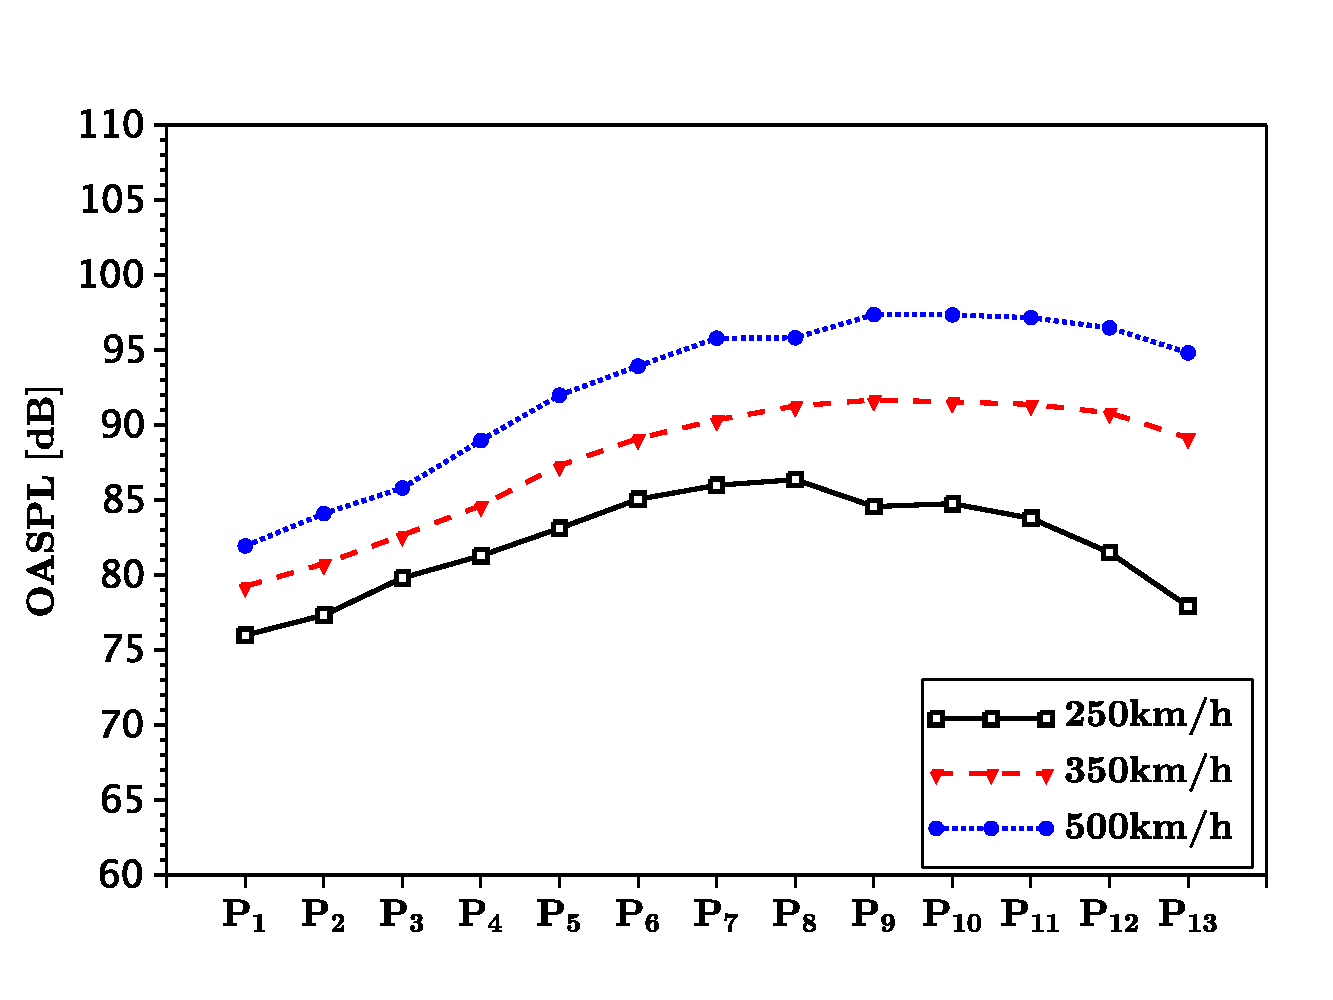
\includegraphics[width=\linewidth]{Figures/oaspl_c.pdf}
    \neusubfigcaption{fig:ch0-side-by-side-a}{工况一}
  \end{neusubfigure}
  \hfill
  \begin{neusubfigure}{0.49\linewidth}
    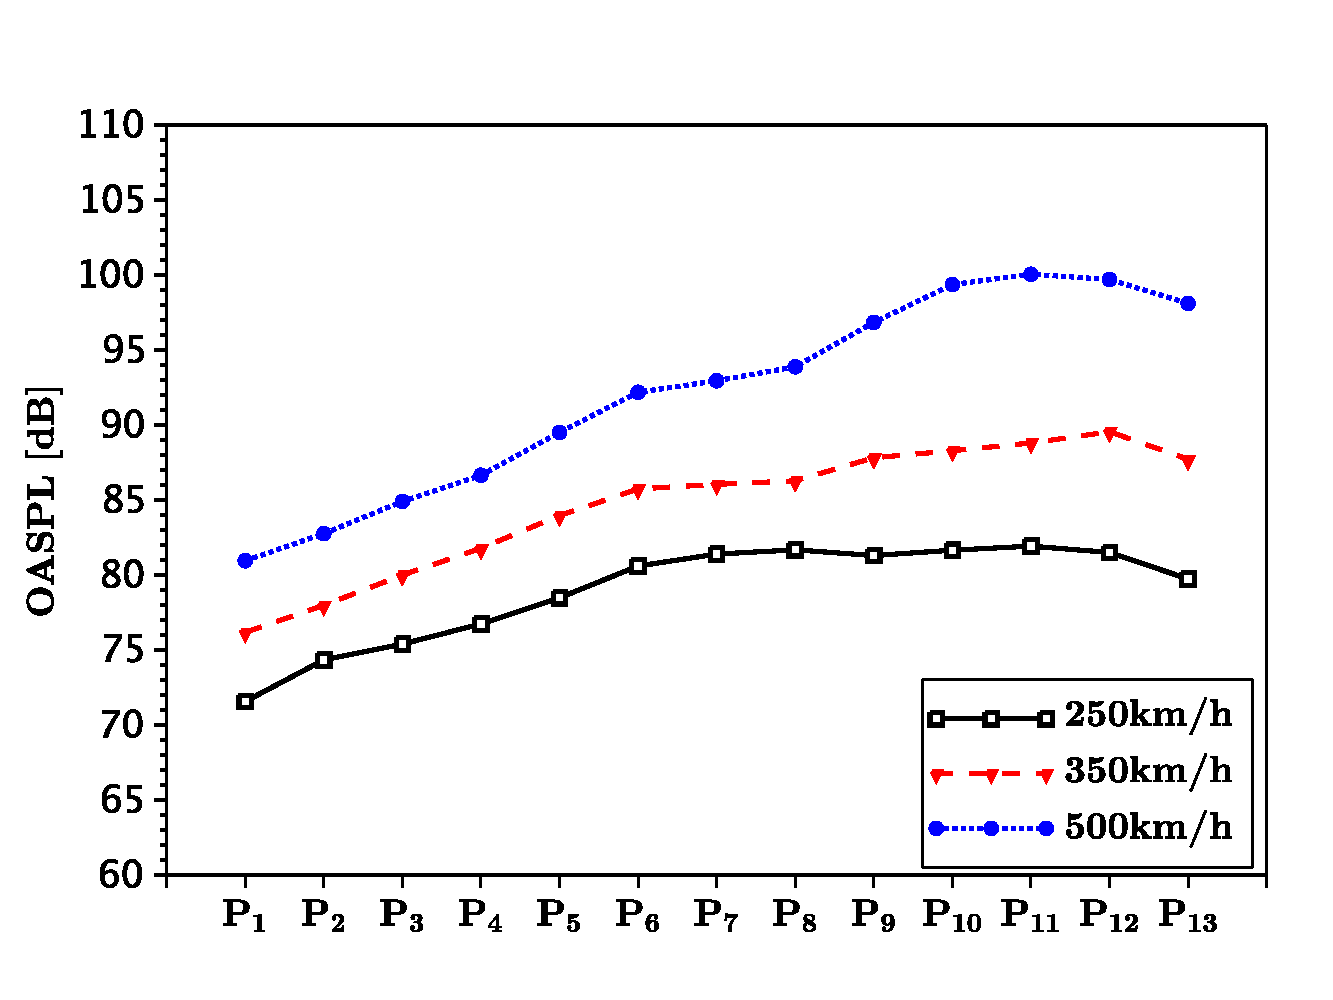
\includegraphics[width=\linewidth]{Figures/oaspl_d.pdf}
    \neusubfigcaption{fig:ch0-side-by-side-b}{工况二}
  \end{neusubfigure}
  \neufigcaption{fig:ch0-subfigures}{并列子图排版样例}{Example of Side-by-Side Subfigures}
\end{figure}

\neufigref{fig:ch0-subfigures} 使用 \texttt{neusubfigure} 完成并列子图排版。
其中 \neusubfigref{fig:ch0-side-by-side-a} 和 \neusubfigref{fig:ch0-side-by-side-b} 可分别引用到子图。
当两幅图共享一个总标题且需要分别引用时，可使用这种方式；如果每幅图需要完全独立的图号，建议拆成两个独立的 \texttt{figure} 环境。

\subsection{二乘二子图}
\begin{figure}[!htbp]
  \centering
  \begin{neusubfigure}{0.49\linewidth}
    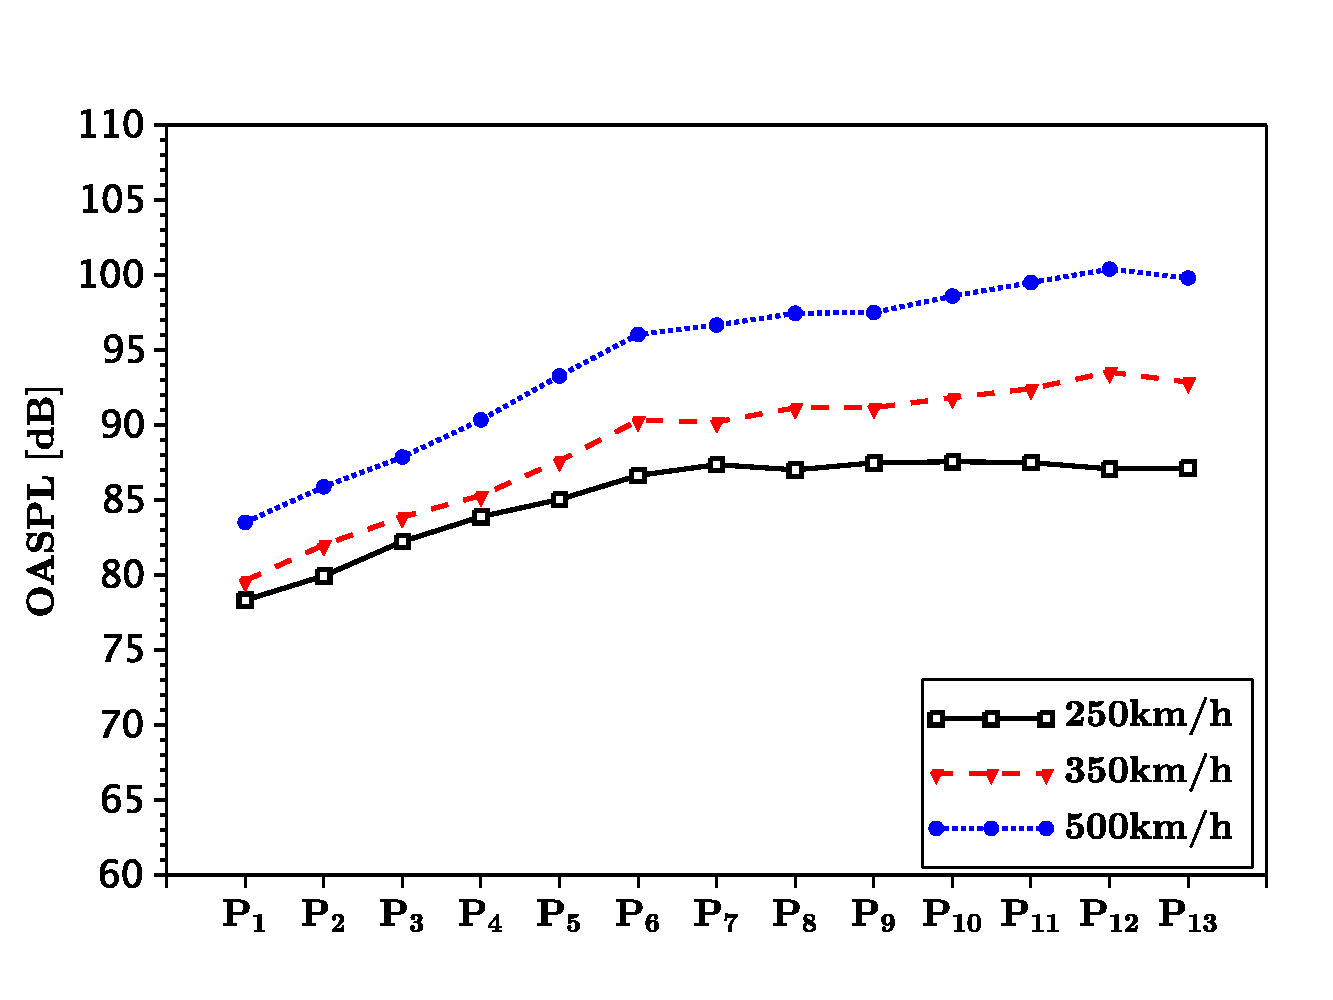
\includegraphics[width=\linewidth]{Figures/oaspl_a.pdf}
    \neusubfigcaption{fig:ch0-four-subfig-a}{工况一}
  \end{neusubfigure}
  \hfill
  \begin{neusubfigure}{0.49\linewidth}
    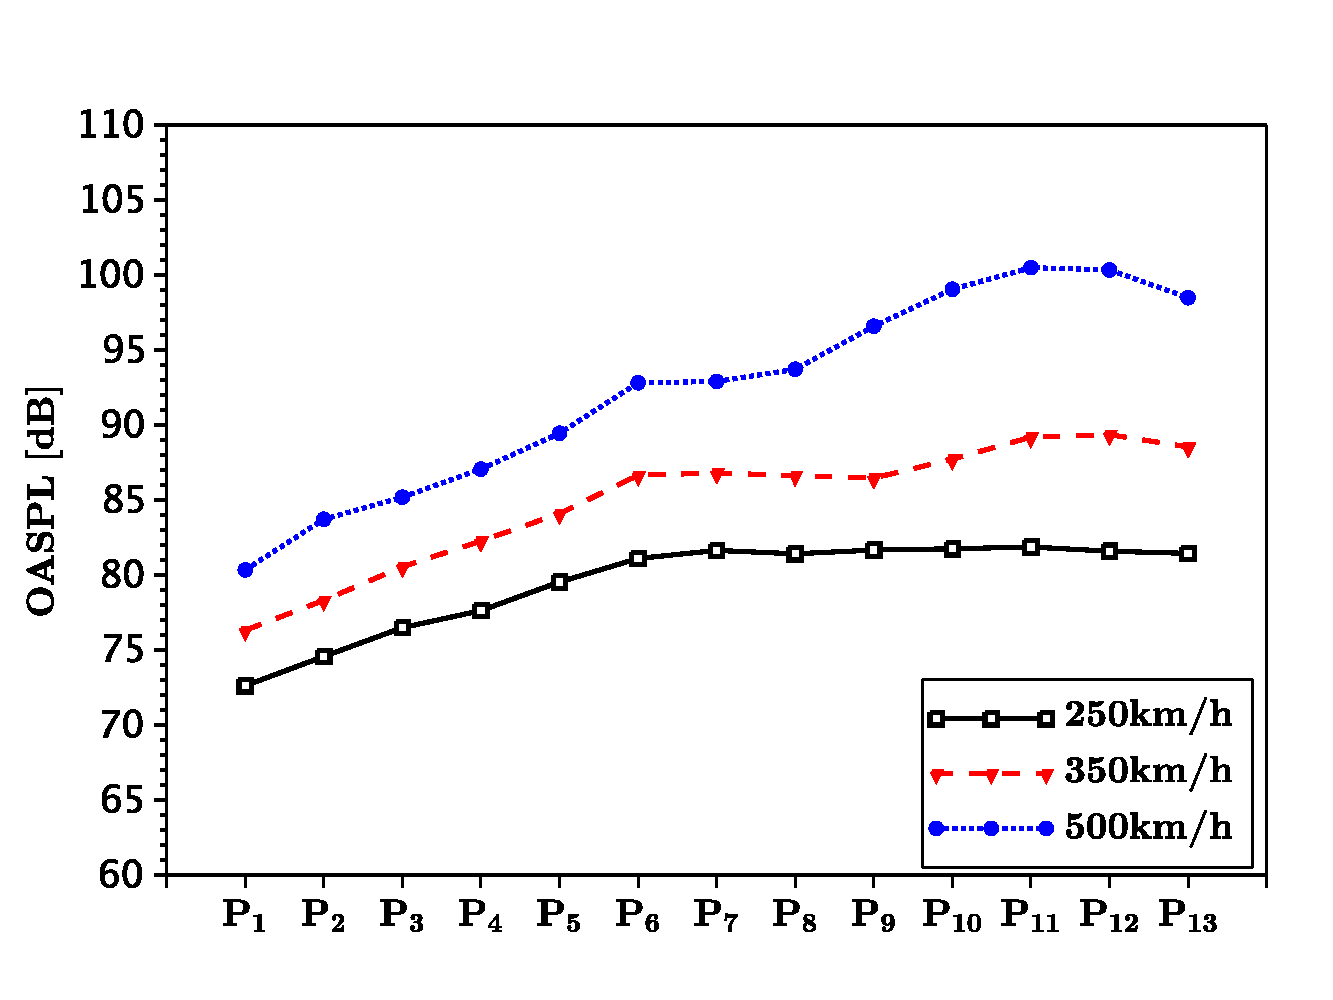
\includegraphics[width=\linewidth]{Figures/oaspl_b.pdf}
    \neusubfigcaption{fig:ch0-four-subfig-b}{工况二}
  \end{neusubfigure}
  \par\vspace{2bp}

  \begin{neusubfigure}{0.49\linewidth}
    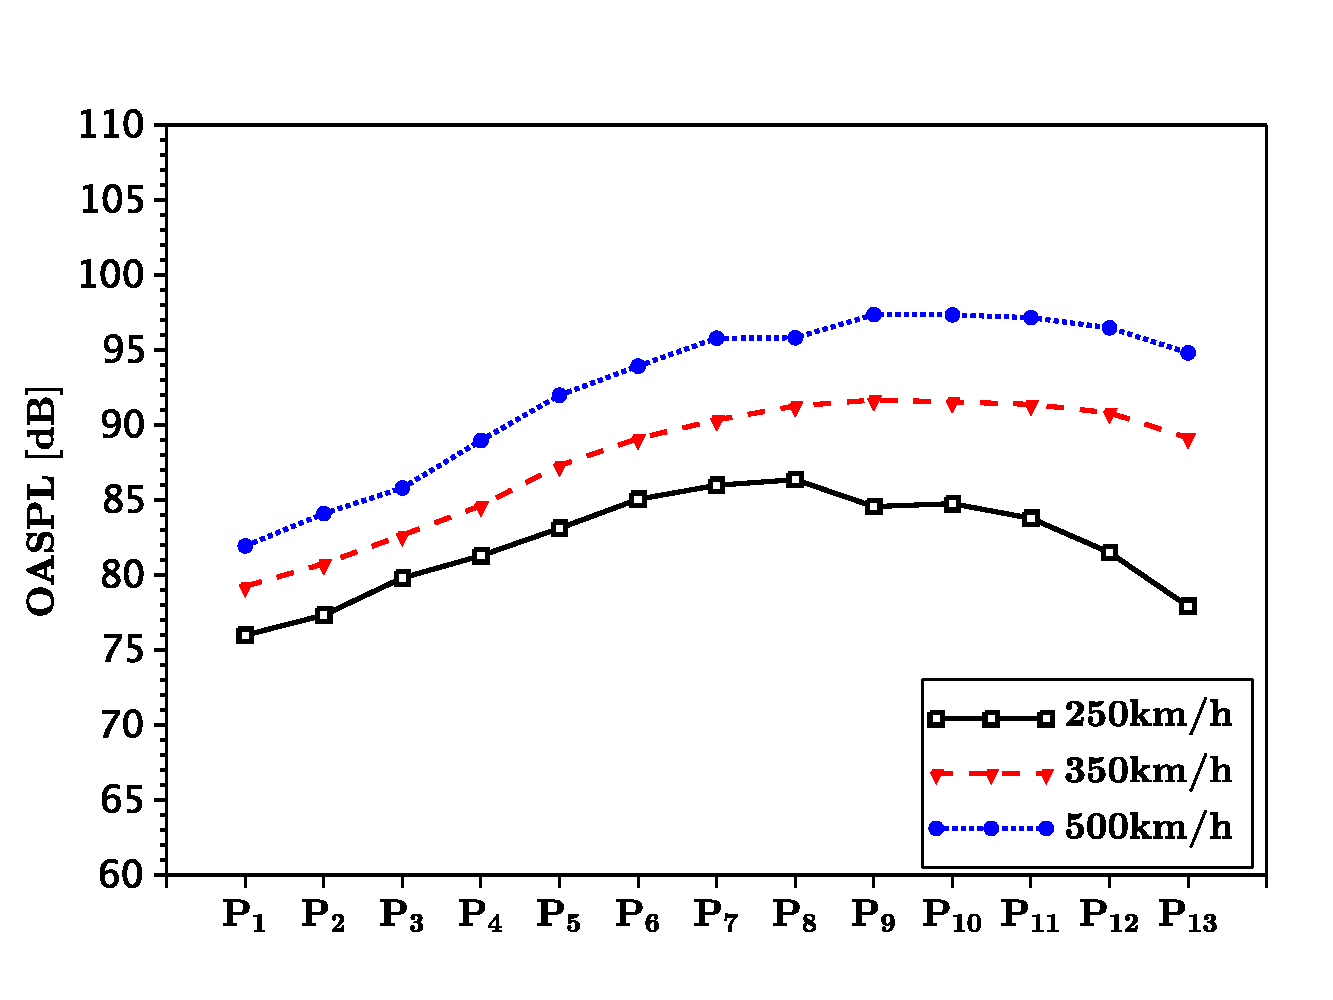
\includegraphics[width=\linewidth]{Figures/oaspl_c.pdf}
    \neusubfigcaption{fig:ch0-four-subfig-c}{工况三}
  \end{neusubfigure}
  \hfill
  \begin{neusubfigure}{0.49\linewidth}
    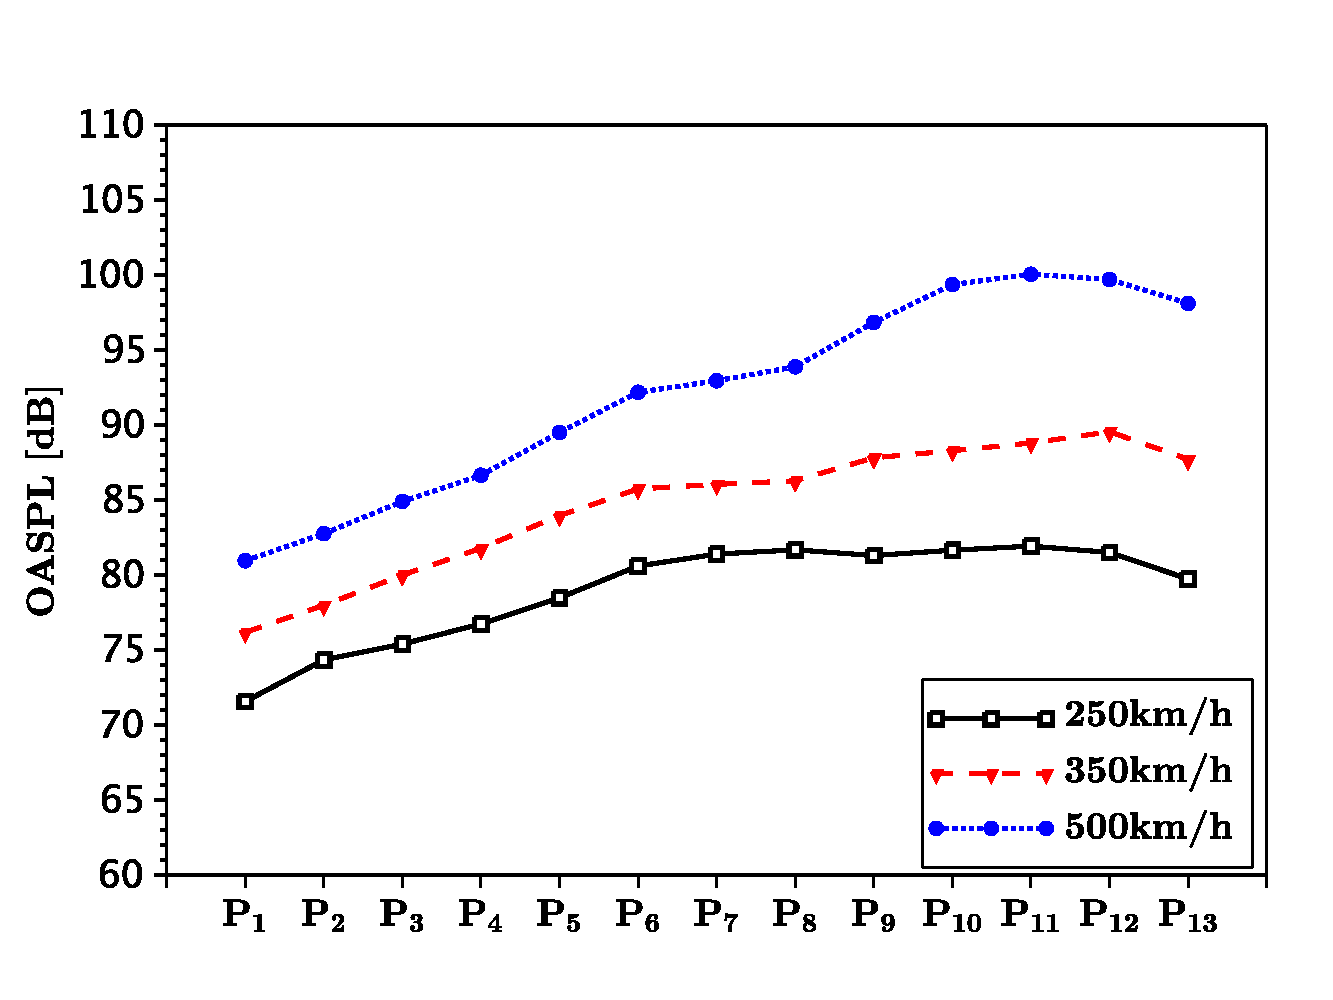
\includegraphics[width=\linewidth]{Figures/oaspl_d.pdf}
    \neusubfigcaption{fig:ch0-four-subfig-d}{工况四}
  \end{neusubfigure}
  \neufigcaption{fig:ch0-four-subfigures}{二乘二子图排版样例}{Example of Two-by-Two Subfigures}
\end{figure}

\neufigref{fig:ch0-four-subfigures} 展示了四幅子图的二乘二排布。
例如 \neusubfigref{fig:ch0-four-subfig-a} 至 \neusubfigref{fig:ch0-four-subfig-d} 可分别引用到四个子图。
排版时建议注意以下几点：
\begin{itemize}
  \item 子图宽度通常可取 \verb|0.48\linewidth| 至 \verb|0.49\linewidth|。
  \item 每行两个子图之间使用 \verb|\hfill| 自动拉开横向间距。
  \item 两行之间可用少量 \verb|\par\vspace| 控制垂直间距。
\end{itemize}

\section{表格排版}

本模板提供 \verb|\neutabcaption{label}{中文题名}{English title}| 用于生成中英文表题。
表题应置于表格上方，正文中使用 \verb|\neutabref{label}| 引用。
表格同样建议使用 \verb|[!htbp]|。如果表格过高导致页底空白，优先考虑缩小字号、调整列宽、拆分表格或使用跨页表格，而不是强制分页。

\subsection{三线表}

\begin{table}[!htbp]
  \centering
  \neutabcaption{tab:ch0-booktabs}{三线表样例}{Example of a Three-Line Table}
  \begin{tabular}{lccc}
    \toprule
    方法       & 准确率（\%）       & 召回率（\%）       & F1 值           \\
    \midrule
    Baseline & 85.2          & 84.1          & 0.846          \\
    Method A & 89.7          & 88.9          & 0.893          \\
    Proposed & \textbf{92.1} & \textbf{91.5} & \textbf{0.918} \\
    \bottomrule
  \end{tabular}
\end{table}

\neutabref{tab:ch0-booktabs} 展示了推荐的三线表格式。
论文中应尽量避免过多竖线，以保持表格简洁。

\subsection{复杂表格}
\begin{table}[!htbp]
  \centering
  \neutabcaption{tab:ch0-complex}{合并单元格与自动换行表格样例}{Example of Merged Cells and Auto-Wrapping Columns}
  \begin{tabularx}{\textwidth}{llXc}
    \toprule
    类别                  & 指标  & 说明                               & 是否必需 \\
    \midrule
    \multirow{2}{*}{图形} & 分辨率 & 位图图片应保证在最终 PDF 中清晰可辨。            & 是    \\
                        & 题名  & 图题使用中英文双语标题，并位于图片下方。             & 是    \\
    \midrule
    \multirow{2}{*}{表格} & 宽度  & 宽表格可使用 \texttt{tabularx} 自动分配列宽。 & 否    \\
                        & 表注  & 表内说明应简明，必要时可在正文中解释。              & 否    \\
    \bottomrule
  \end{tabularx}
\end{table}

\neutabref{tab:ch0-complex} 同时展示了 \verb|\multirow|、\verb|\makecell| 可配合使用的复杂表格场景。
若单元格内容较长，优先使用 \texttt{tabularx} 或 \texttt{p\{...\}} 列类型控制宽度。

\section{公式排版}

公式应使用标准数学环境，并通过 \verb|\label| 设置标签。
引用公式时建议使用模板提供的 \verb|\neueqref{label}|。

\subsection{单行公式}
以分类任务中的交叉熵损失为例，可写为
\begin{equation}
  \mathcal{L}(\theta)
  = - \frac{1}{N}\sum_{i=1}^{N}\sum_{k=1}^{K} y_{ik}\log p_{ik}
  \label{eq:ch0-loss}
\end{equation}

如 \neueqref{eq:ch0-loss} 所示，带编号公式适合放置正文中需要引用的重要定义。

\subsection{多行公式}
循环模型中的状态更新和输出计算可写为
\begin{align}
  h_t       & = \sigma(W_x x_t + W_h h_{t-1} + b), \label{eq:ch0-state} \\
  \hat{y}_t & = \operatorname{softmax}(W_o h_t). \label{eq:ch0-output}
\end{align}

\neueqref{eq:ch0-state} 和 \neueqref{eq:ch0-output} 展示了多行公式的编号方式。
如果多行推导只需要一个编号，可使用 \texttt{aligned} 放在 \texttt{equation} 环境内部。

\subsection{分段函数与矩阵}
分段函数和矩阵经常同时出现在数学定义中，例如
\begin{equation}
  g(x)=
  \begin{cases}
    0, & x < 0,       \\
    x, & 0 \le x < 1, \\
    1, & x \ge 1,
  \end{cases}
  \qquad
  A =
  \begin{bmatrix}
    1 & 0 & 0 \\
    0 & 1 & 0 \\
    0 & 0 & 1
  \end{bmatrix}.
  \label{eq:ch0-piecewise}
\end{equation}

\neueqref{eq:ch0-piecewise} 展示了分段函数和矩阵的常见写法。

\section{算法伪代码}

计算机类论文常需要给出算法步骤。本文档在 \texttt{main.tex} 中加载了 \texttt{algorithm} 和 \texttt{algorithmic} 宏包，可以直接使用如下环境。

\begin{algorithm}[!htbp]
  \caption{样例训练流程}
  \label{alg:ch0-training}
  \begin{algorithmic}[1]
    \REQUIRE Training set $\mathcal{D}$, learning rate $\eta$, maximum epoch $T$
    \ENSURE Model parameters $\theta$
    \STATE Initialize parameters $\theta$
    \FOR{$t = 1$ to $T$}
    \STATE Sample a mini-batch $\mathcal{B}$ from $\mathcal{D}$
    \STATE Compute loss $\mathcal{L}(\theta)$ by \neueqref{eq:ch0-loss}
    \STATE Update $\theta \leftarrow \theta - \eta \nabla_{\theta}\mathcal{L}(\theta)$
    \ENDFOR
    \RETURN $\theta$
  \end{algorithmic}
\end{algorithm}

算法~\ref{alg:ch0-training} 展示了带行号的伪代码。
若需要中文关键字，可在导言区重定义相应命令。

\section{引用、链接与交叉引用}

参考文献引用可使用两种模板命令：
\begin{itemize}
  \item 上标引用使用 \verb|\upcite{key}|，适合放在句末，例如已有研究讨论了神经网络轻量化问题\upcite{guo_2023_research}。
  \item 正文引用使用 \verb|\inlinecite{key}|，适合作为句子成分，例如文献 \inlinecite{thakkar_2018_performance} 给出了系统性能评测案例。
\end{itemize}
多篇文献可写在同一条引用命令中，例如区块链平台相关研究\upcite{zheng_2019_nutbaas,thakkar_2018_performance}。

交叉引用建议统一使用模板命令：
\begin{itemize}
  \item 图引用：\verb|\neufigref{fig:ch0-pdf}|，效果为 \neufigref{fig:ch0-pdf}。
  \item 子图引用：\verb|\neusubfigref{fig:ch0-four-subfig-a}|，效果为 \neusubfigref{fig:ch0-four-subfig-a}。
  \item 表引用：\verb|\neutabref{tab:ch0-complex}|，效果为 \neutabref{tab:ch0-complex}。
  \item 公式引用：\verb|\neueqref{eq:ch0-loss}|，效果为 \neueqref{eq:ch0-loss}。
  \item 算法引用：当前模板未单独封装算法引用命令，可写作“算法~\ref{alg:ch0-training}”。
\end{itemize}
模板提供的公开命令和环境可参考 \texttt{README.md} 中的“模板命令说明”一节。
|。
脚注示例如此处所示\footnote{脚注用于补充说明，不宜放置过长的正文内容。}。
若某页因图表浮动或分页规则没有排满，脚注可能跟随正文排版区而显得略高，这是正常的 LaTeX 页面构建结果。

\subsection{字体、字号与强调}

模板预定义了常用中文字体命令。正式论文中通常不需要手动切换字体；只有在展示样式、术语强调或特殊说明时才建议使用。
当前模板已经为默认宋体和 \verb|\song| 字族配置伪粗体，因此 \verb|\textbf| 或 \verb|\bfseries| 可以用于中文局部强调。
需要注意的是，中文加粗应克制使用；标题层级、术语定义或表格重点值可以适当加粗，大段正文不建议整体加粗。
如果需要更明显的标题式强调，可使用黑体或调整标题层级；如果只是普通正文重点，优先使用 \verb|\textbf|。

\begin{table}[!htbp]
  \centering
  \neutabcaption{tab:ch0-fonts}{字体与强调样例}{Examples of Fonts and Emphasis}
  \begin{tabular}{lll}
    \toprule
    命令             & 显示效果                         & 使用建议       \\
    \midrule
    \verb|\song|   & {\song 宋体文字示例}               & 正文默认字体     \\
    \verb|\textbf| & \textbf{加粗文字示例}              & 局部强调、表格重点值 \\
    \verb|\hei|    & {\hei 黑体文字示例}                & 标题或较强强调场景  \\
    \verb|\kai|    & {\kai 楷体文字示例}                & 摘要、题签或引用语  \\
    \verb|\fs|     & {\fs 仿宋文字示例}                 & 特殊文书类内容    \\
    \verb|\textit| & \textit{Italic text example} & 英文斜体或变量说明  \\
    \bottomrule
  \end{tabular}
\end{table}

\subsection{列表环境}

无序列表适合列出并列事项：
\begin{itemize}
  \item 图题位于图下方，表题位于表上方。
  \item 图表应使用中英文双语标题。
  \item 公式、图、表、算法均应使用标签进行交叉引用。
\end{itemize}

有序列表适合描述步骤：
\begin{enumerate}
  \item 在 \texttt{main.tex} 中填写论文元信息。
  \item 在各章文件中撰写正文内容。
  \item 使用 \texttt{latexmk -xelatex main.tex} 完成编译。
\end{enumerate}

\section{图形排版}

本模板提供 \verb|\neufigcaption{label}{中文题名}{English title}| 用于生成中英文图题。
图题应置于图形下方，正文中使用 \verb|\neufigref{label}| 引用。
图形建议使用 \verb|[!htbp]| 浮动参数，让 LaTeX 在当前位置、页顶、页底或浮动页中选择较合适的位置；除非必须固定位置，否则不建议使用 \verb|[H]|。

\subsection{外部图片}
\begin{figure}[!htbp]
  \centering
  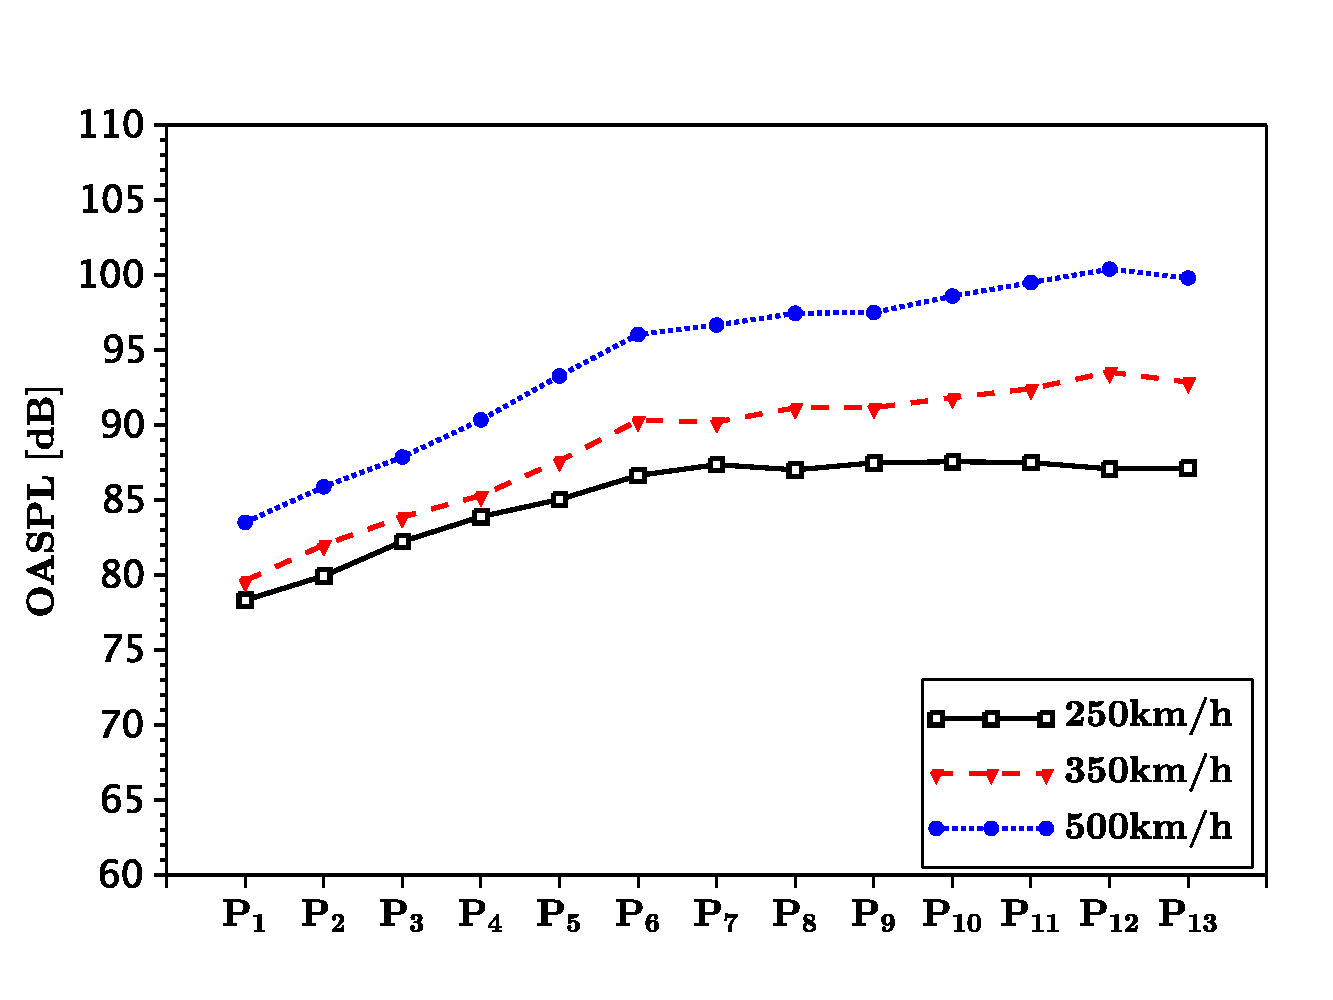
\includegraphics[width=0.55\textwidth]{Figures/oaspl_a.pdf}
  \neufigcaption{fig:ch0-cover}{外部图片插入样例}{Example of Including an External Image}
\end{figure}

\neufigref{fig:ch0-cover} 展示了通过 \verb|\includegraphics| 插入图片文件的方式。
正式论文中建议将图片统一放入 \texttt{Figures} 目录，并使用相对路径引用。

\subsection{PDF 或位图图片}
\begin{figure}[!htbp]
  \centering
  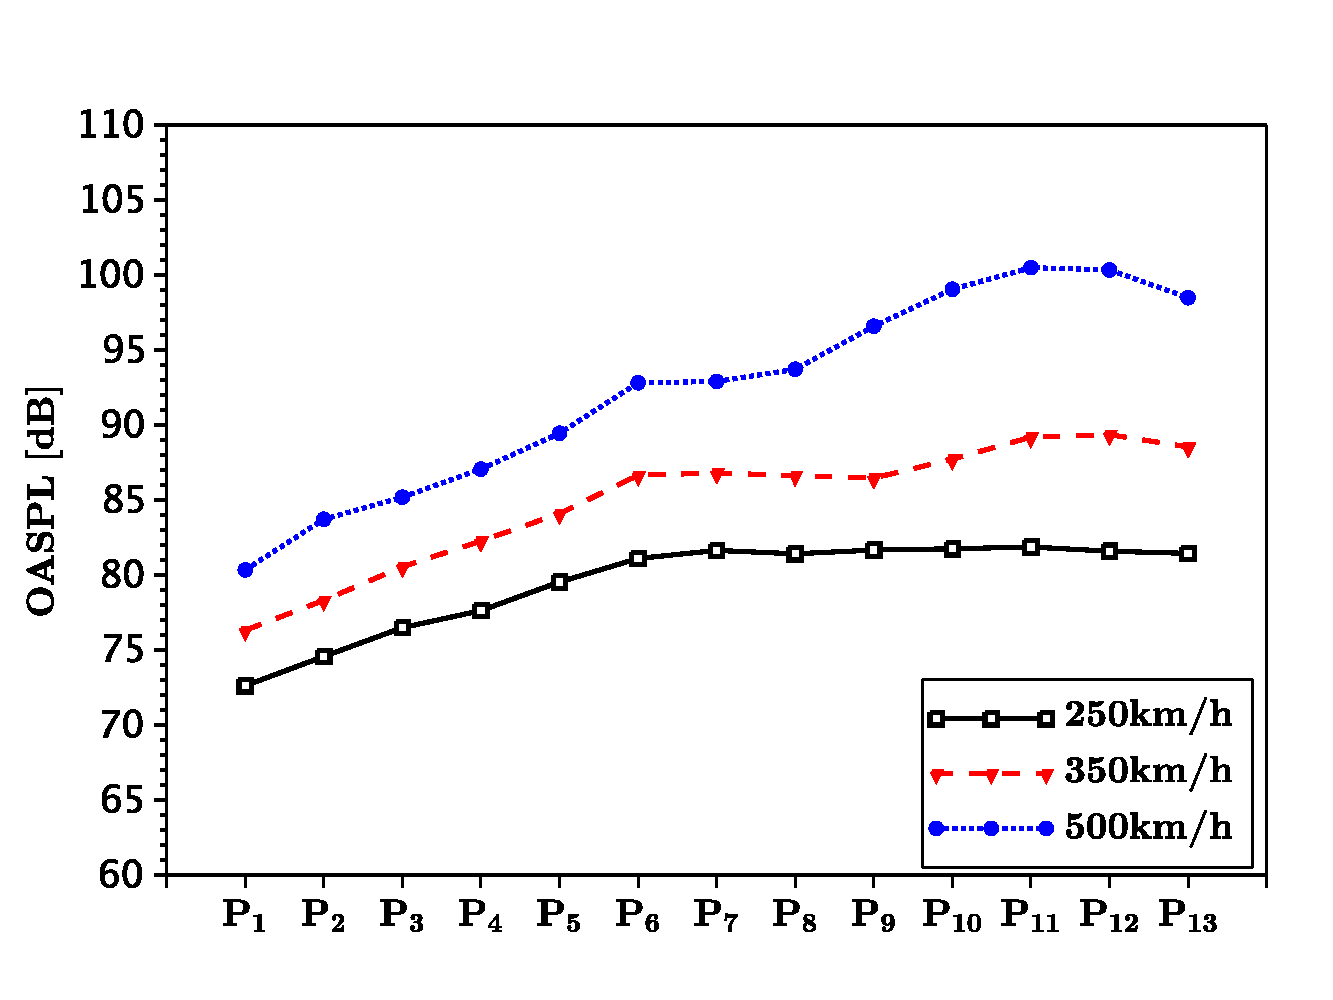
\includegraphics[width=0.55\textwidth]{Figures/oaspl_b.pdf}
  \neufigcaption{fig:ch0-pdf}{PDF 图片插入样例}{Example of Including a PDF Figure}
\end{figure}

PDF、PNG、JPG 等常见图片格式均可通过 \verb|\includegraphics| 插入。
若图片由绘图软件或数据分析程序导出，建议优先使用 PDF 格式以保持较清晰的显示效果。

\subsection{并列图片}
\begin{figure}[!htbp]
  \centering
  \begin{minipage}[t]{0.49\linewidth}
    \centering
    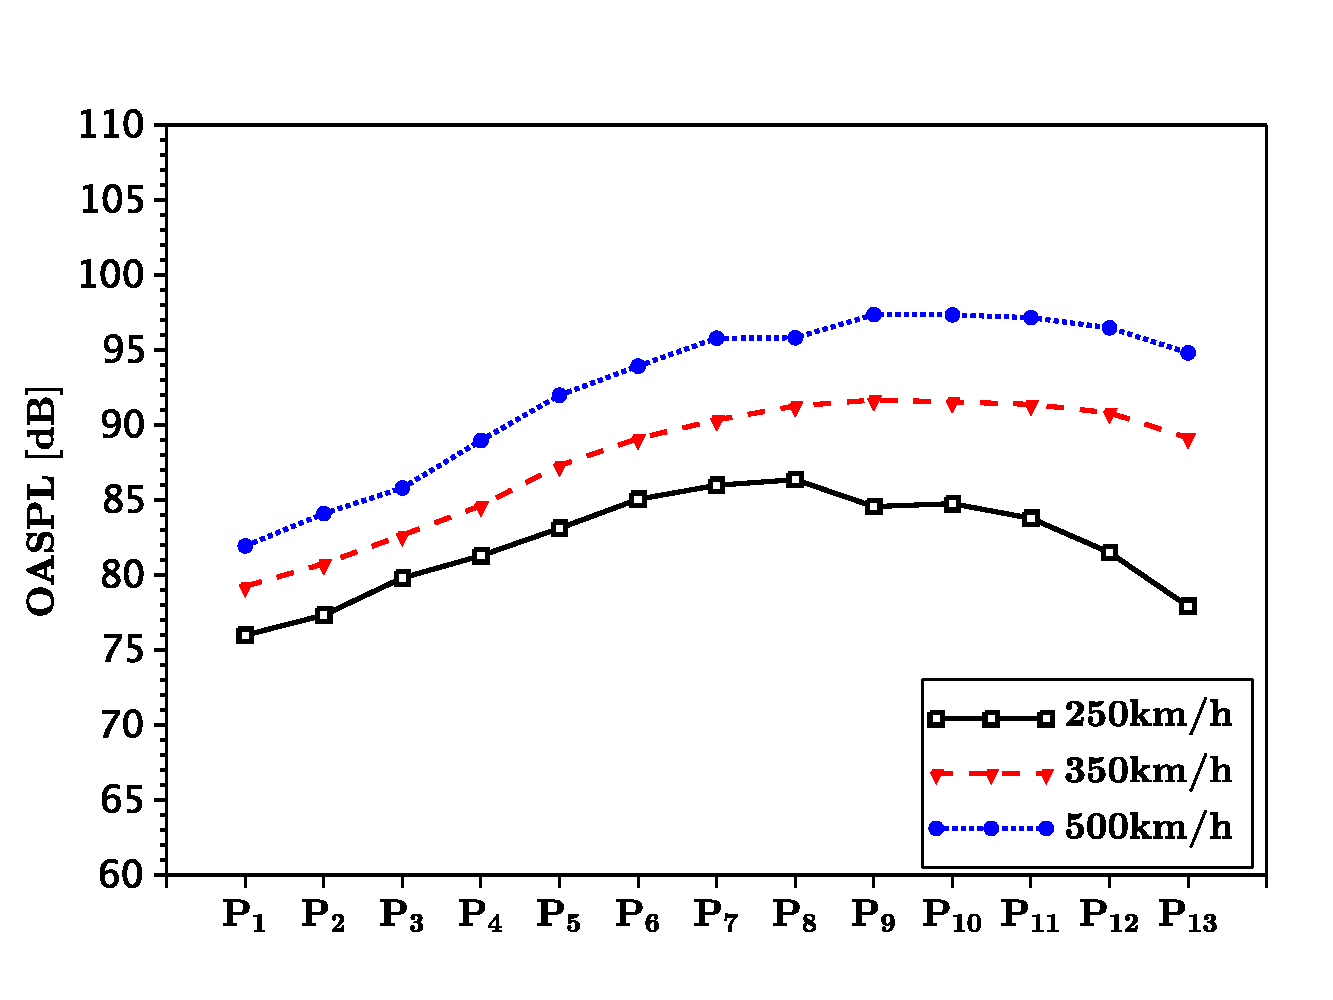
\includegraphics[width=\linewidth]{Figures/oaspl_c.pdf}
  \end{minipage}
  \hfill
  \begin{minipage}[t]{0.49\linewidth}
    \centering
    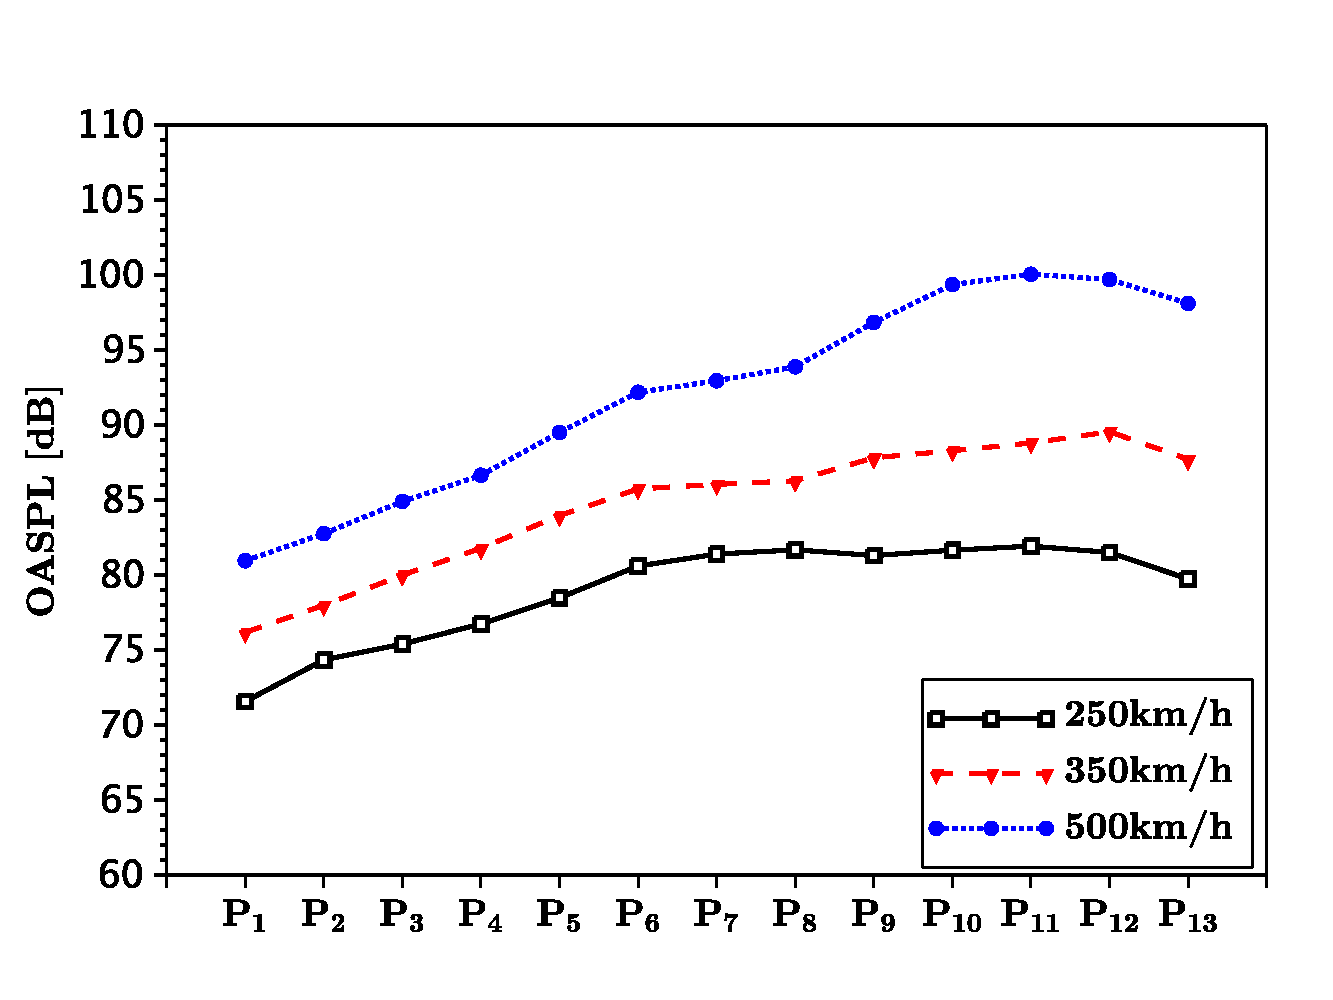
\includegraphics[width=\linewidth]{Figures/oaspl_d.pdf}
  \end{minipage}
  \neufigcaption{fig:ch0-side-by-side}{普通并列图形排版样例}{Example of Side-by-Side Figures}
\end{figure}

\neufigref{fig:ch0-side-by-side} 使用 \texttt{minipage} 完成普通并列排版。
当两幅图共享一个总标题且不需要分别引用时，可使用这种方式。

\subsection{并列子图}
\begin{figure}[!htbp]
  \centering
  \begin{neusubfigure}{0.49\linewidth}
    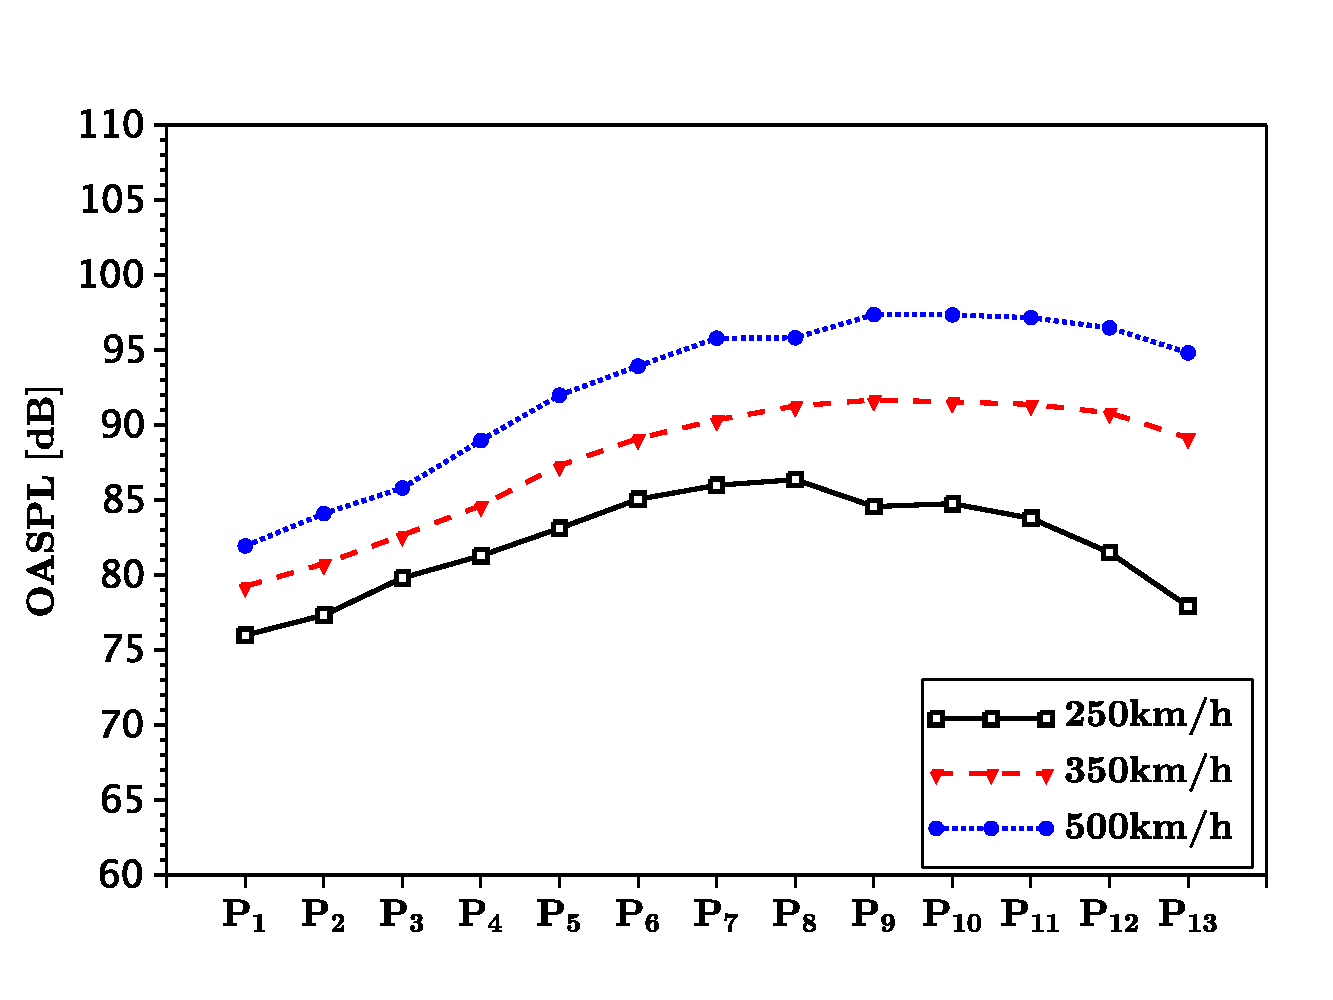
\includegraphics[width=\linewidth]{Figures/oaspl_c.pdf}
    \neusubfigcaption{fig:ch0-side-by-side-a}{工况一}
  \end{neusubfigure}
  \hfill
  \begin{neusubfigure}{0.49\linewidth}
    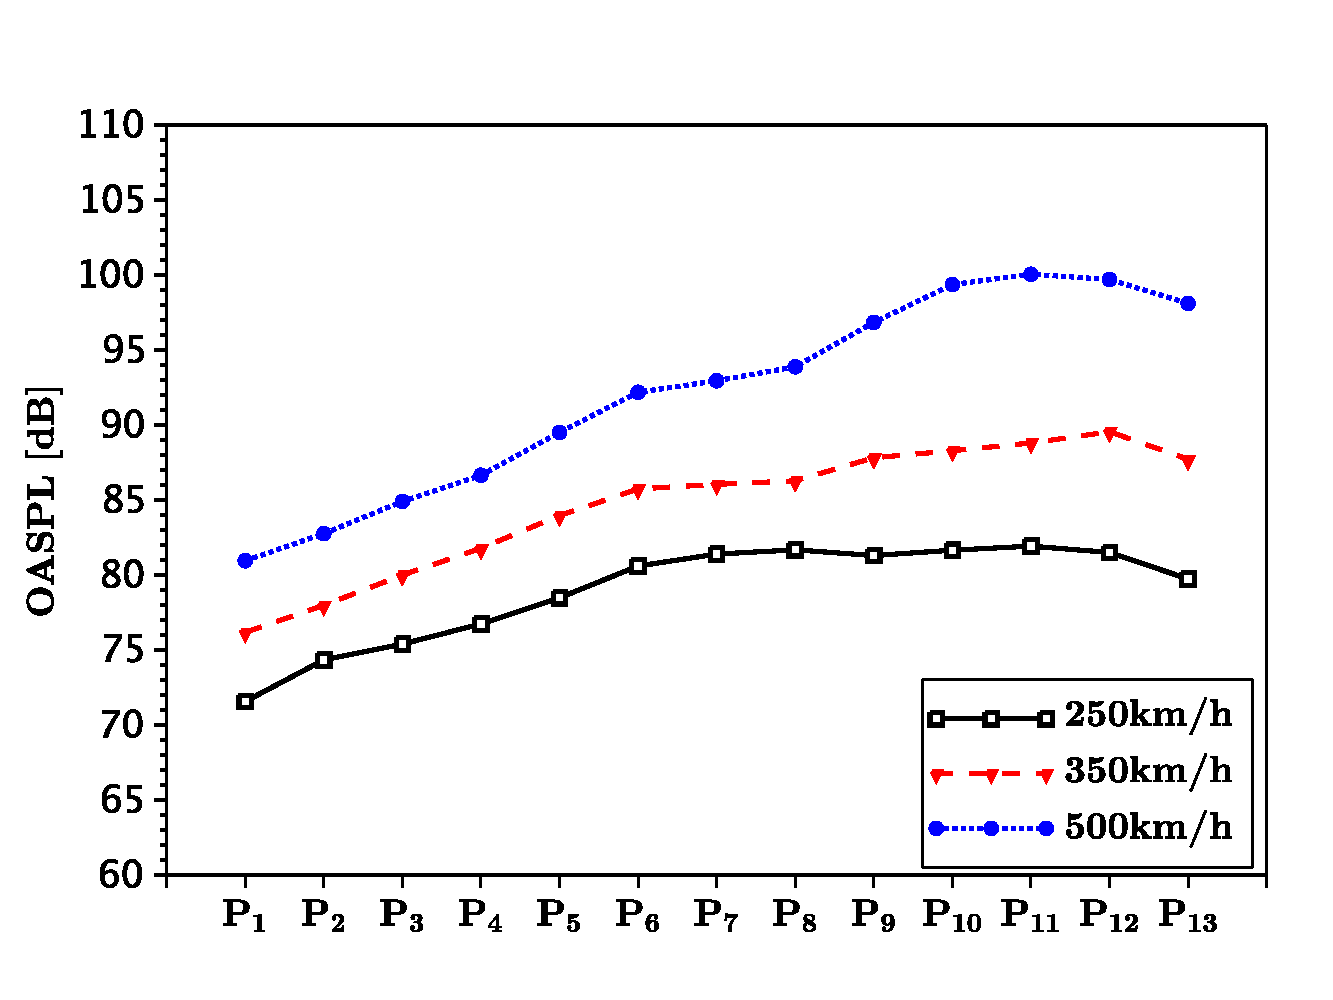
\includegraphics[width=\linewidth]{Figures/oaspl_d.pdf}
    \neusubfigcaption{fig:ch0-side-by-side-b}{工况二}
  \end{neusubfigure}
  \neufigcaption{fig:ch0-subfigures}{并列子图排版样例}{Example of Side-by-Side Subfigures}
\end{figure}

\neufigref{fig:ch0-subfigures} 使用 \texttt{neusubfigure} 完成并列子图排版。
其中 \neusubfigref{fig:ch0-side-by-side-a} 和 \neusubfigref{fig:ch0-side-by-side-b} 可分别引用到子图。
当两幅图共享一个总标题且需要分别引用时，可使用这种方式；如果每幅图需要完全独立的图号，建议拆成两个独立的 \texttt{figure} 环境。

\subsection{二乘二子图}
\begin{figure}[!htbp]
  \centering
  \begin{neusubfigure}{0.49\linewidth}
    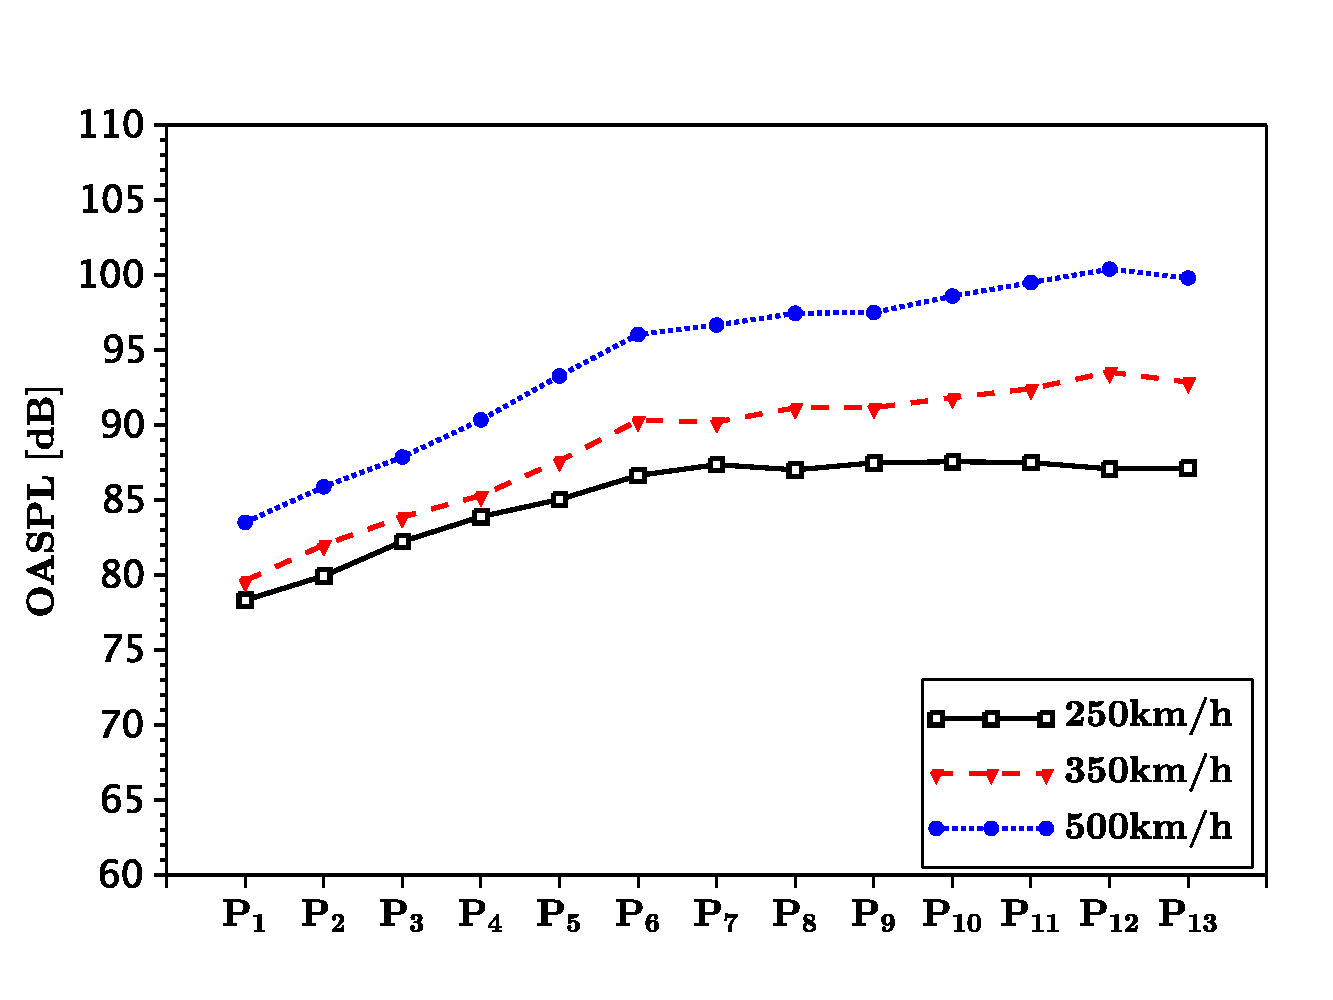
\includegraphics[width=\linewidth]{Figures/oaspl_a.pdf}
    \neusubfigcaption{fig:ch0-four-subfig-a}{工况一}
  \end{neusubfigure}
  \hfill
  \begin{neusubfigure}{0.49\linewidth}
    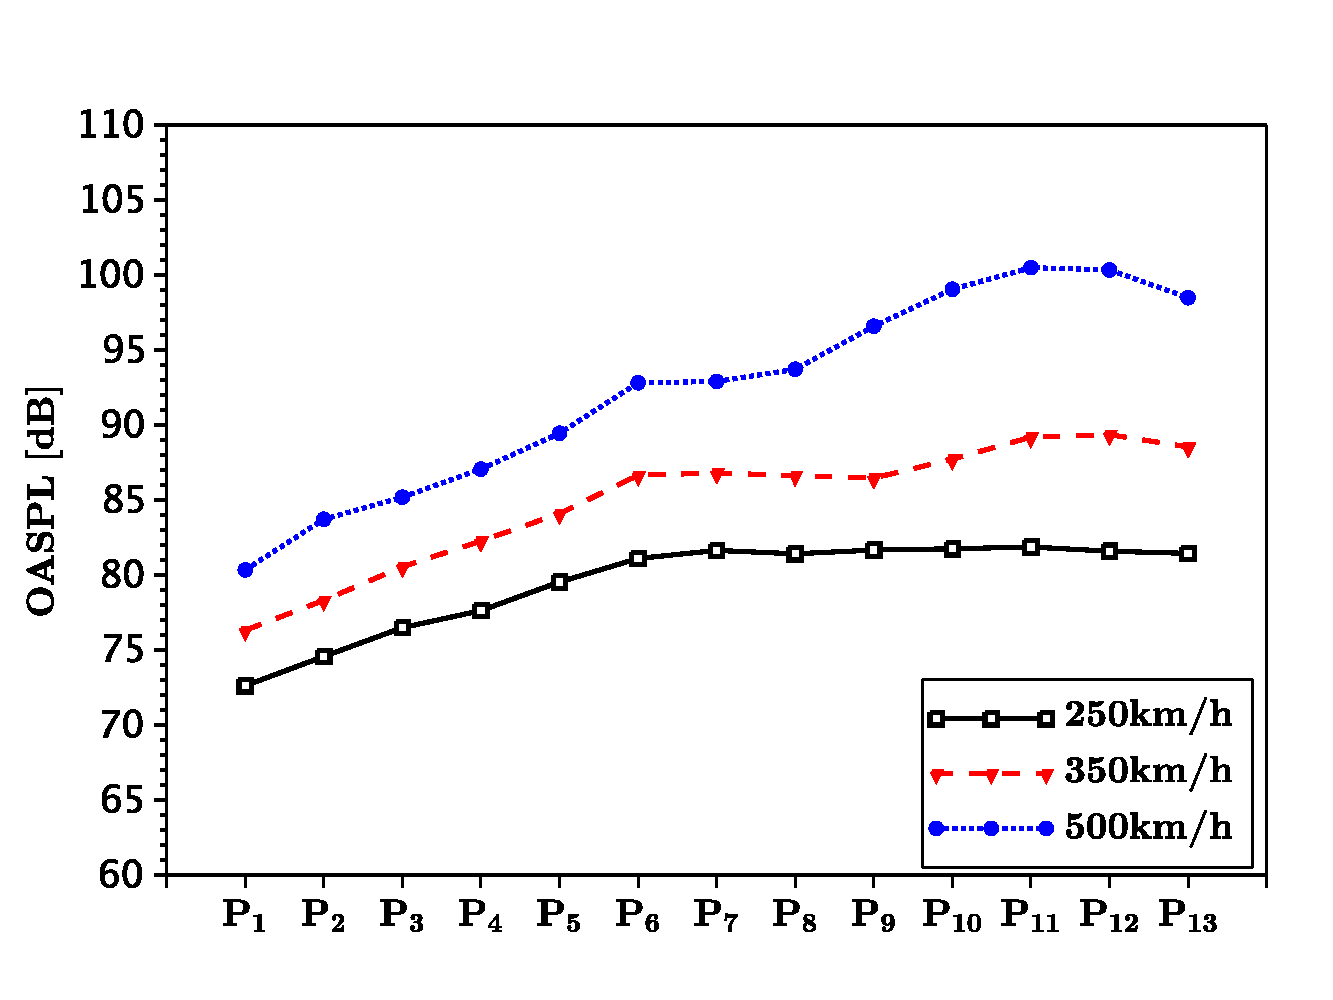
\includegraphics[width=\linewidth]{Figures/oaspl_b.pdf}
    \neusubfigcaption{fig:ch0-four-subfig-b}{工况二}
  \end{neusubfigure}
  \par\vspace{2bp}

  \begin{neusubfigure}{0.49\linewidth}
    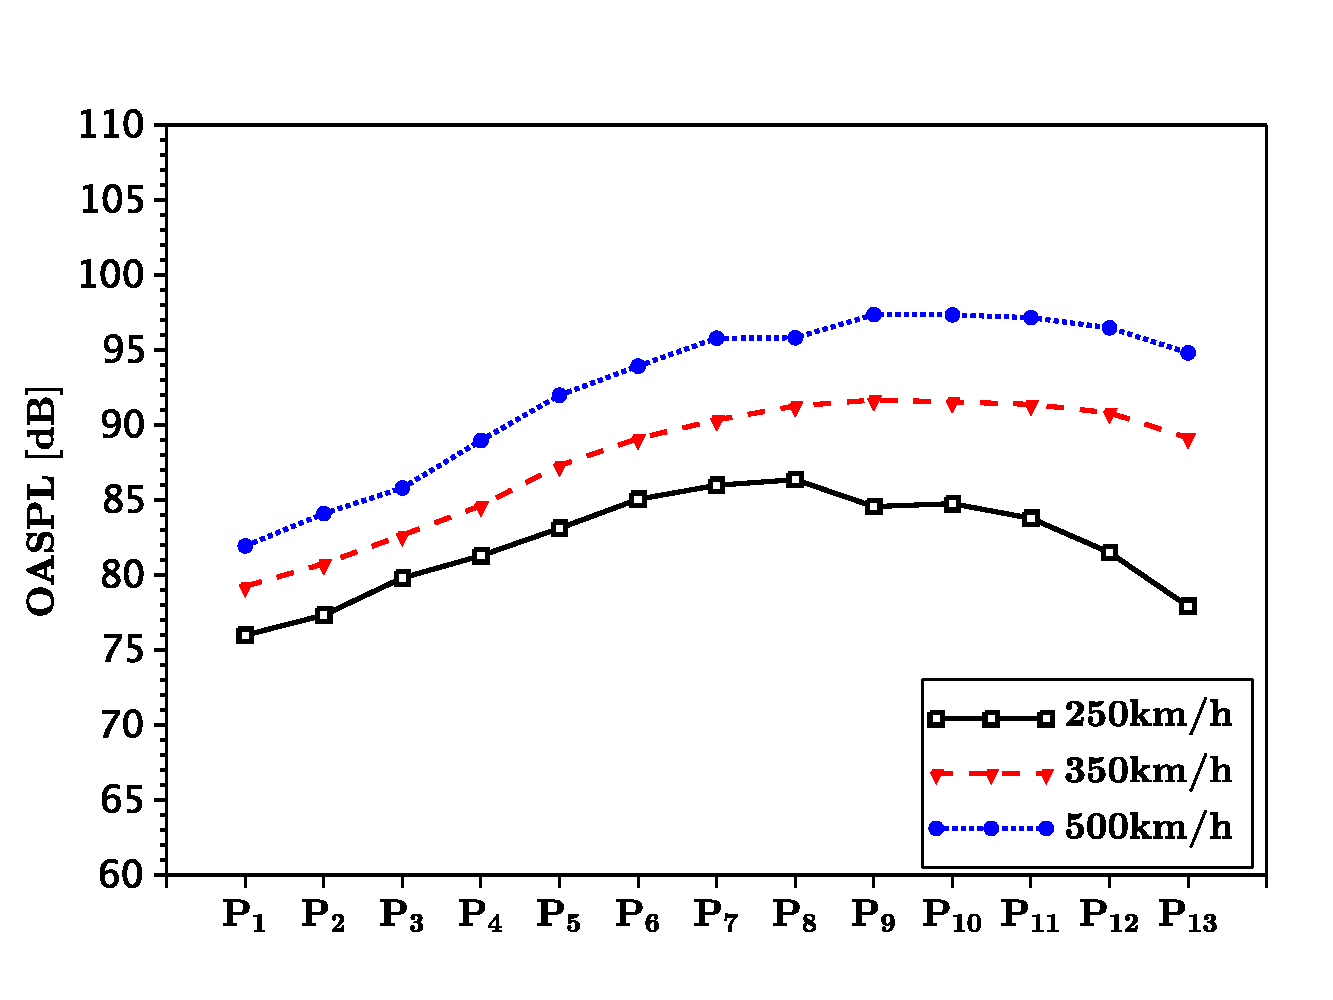
\includegraphics[width=\linewidth]{Figures/oaspl_c.pdf}
    \neusubfigcaption{fig:ch0-four-subfig-c}{工况三}
  \end{neusubfigure}
  \hfill
  \begin{neusubfigure}{0.49\linewidth}
    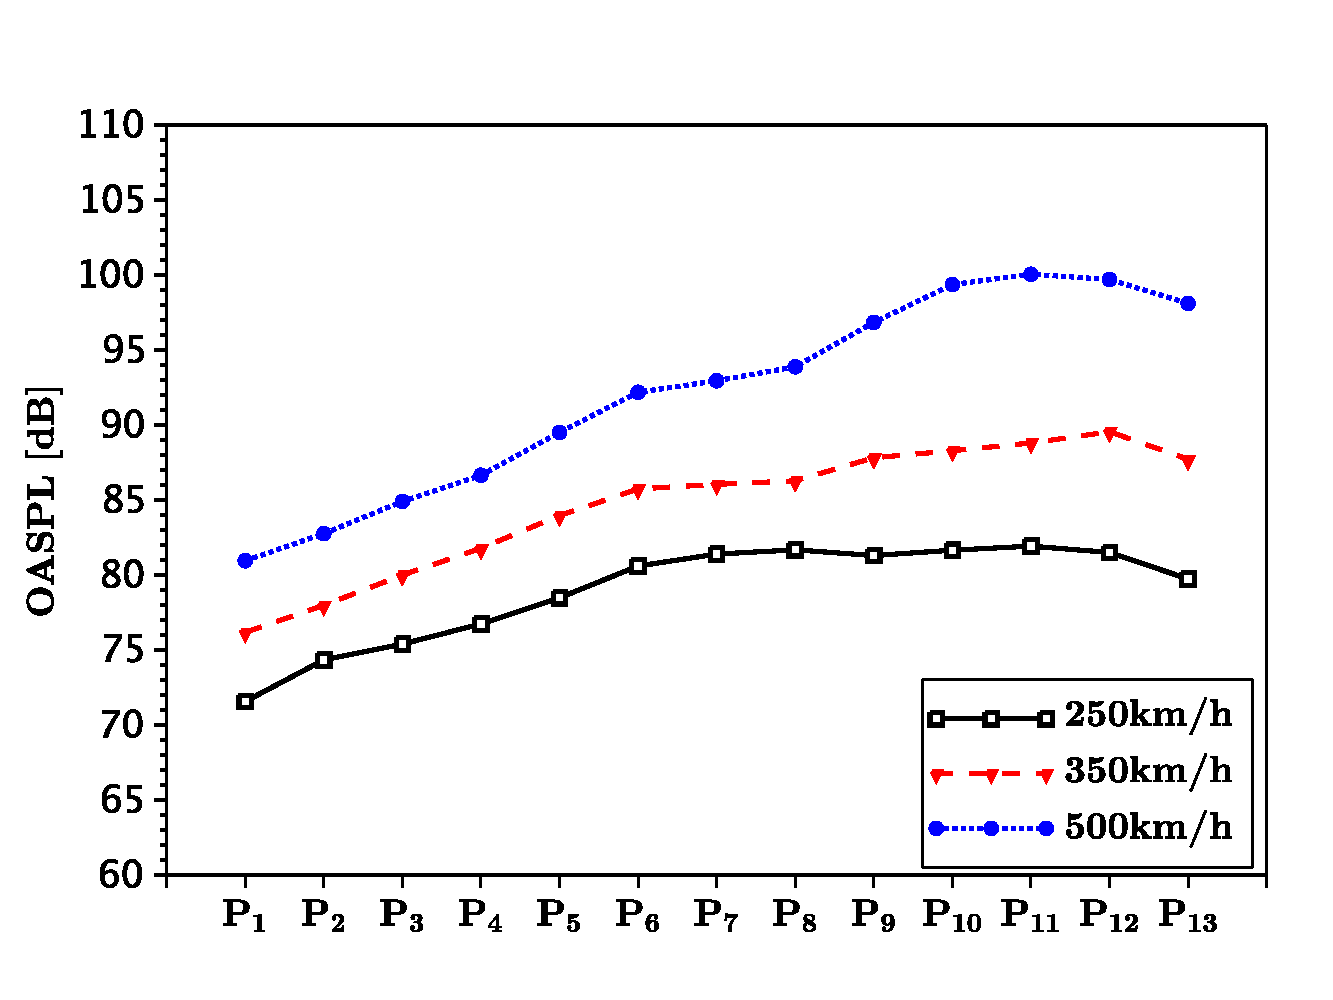
\includegraphics[width=\linewidth]{Figures/oaspl_d.pdf}
    \neusubfigcaption{fig:ch0-four-subfig-d}{工况四}
  \end{neusubfigure}
  \neufigcaption{fig:ch0-four-subfigures}{二乘二子图排版样例}{Example of Two-by-Two Subfigures}
\end{figure}

\neufigref{fig:ch0-four-subfigures} 展示了四幅子图的二乘二排布。
例如 \neusubfigref{fig:ch0-four-subfig-a} 至 \neusubfigref{fig:ch0-four-subfig-d} 可分别引用到四个子图。
排版时建议注意以下几点：
\begin{itemize}
  \item 子图宽度通常可取 \verb|0.48\linewidth| 至 \verb|0.49\linewidth|。
  \item 每行两个子图之间使用 \verb|\hfill| 自动拉开横向间距。
  \item 两行之间可用少量 \verb|\par\vspace| 控制垂直间距。
\end{itemize}

\section{表格排版}

本模板提供 \verb|\neutabcaption{label}{中文题名}{English title}| 用于生成中英文表题。
表题应置于表格上方，正文中使用 \verb|\neutabref{label}| 引用。
表格同样建议使用 \verb|[!htbp]|。如果表格过高导致页底空白，优先考虑缩小字号、调整列宽、拆分表格或使用跨页表格，而不是强制分页。

\subsection{三线表}

\begin{table}[!htbp]
  \centering
  \neutabcaption{tab:ch0-booktabs}{三线表样例}{Example of a Three-Line Table}
  \begin{tabular}{lccc}
    \toprule
    方法       & 准确率（\%）       & 召回率（\%）       & F1 值           \\
    \midrule
    Baseline & 85.2          & 84.1          & 0.846          \\
    Method A & 89.7          & 88.9          & 0.893          \\
    Proposed & \textbf{92.1} & \textbf{91.5} & \textbf{0.918} \\
    \bottomrule
  \end{tabular}
\end{table}

\neutabref{tab:ch0-booktabs} 展示了推荐的三线表格式。
论文中应尽量避免过多竖线，以保持表格简洁。

\subsection{复杂表格}
\begin{table}[!htbp]
  \centering
  \neutabcaption{tab:ch0-complex}{合并单元格与自动换行表格样例}{Example of Merged Cells and Auto-Wrapping Columns}
  \begin{tabularx}{\textwidth}{llXc}
    \toprule
    类别                  & 指标  & 说明                               & 是否必需 \\
    \midrule
    \multirow{2}{*}{图形} & 分辨率 & 位图图片应保证在最终 PDF 中清晰可辨。            & 是    \\
                        & 题名  & 图题使用中英文双语标题，并位于图片下方。             & 是    \\
    \midrule
    \multirow{2}{*}{表格} & 宽度  & 宽表格可使用 \texttt{tabularx} 自动分配列宽。 & 否    \\
                        & 表注  & 表内说明应简明，必要时可在正文中解释。              & 否    \\
    \bottomrule
  \end{tabularx}
\end{table}

\neutabref{tab:ch0-complex} 同时展示了 \verb|\multirow|、\verb|\makecell| 可配合使用的复杂表格场景。
若单元格内容较长，优先使用 \texttt{tabularx} 或 \texttt{p\{...\}} 列类型控制宽度。

\section{公式排版}

公式应使用标准数学环境，并通过 \verb|\label| 设置标签。
引用公式时建议使用模板提供的 \verb|\neueqref{label}|。

\subsection{单行公式}
以分类任务中的交叉熵损失为例，可写为
\begin{equation}
  \mathcal{L}(\theta)
  = - \frac{1}{N}\sum_{i=1}^{N}\sum_{k=1}^{K} y_{ik}\log p_{ik}
  \label{eq:ch0-loss}
\end{equation}

如 \neueqref{eq:ch0-loss} 所示，带编号公式适合放置正文中需要引用的重要定义。

\subsection{多行公式}
循环模型中的状态更新和输出计算可写为
\begin{align}
  h_t       & = \sigma(W_x x_t + W_h h_{t-1} + b), \label{eq:ch0-state} \\
  \hat{y}_t & = \operatorname{softmax}(W_o h_t). \label{eq:ch0-output}
\end{align}

\neueqref{eq:ch0-state} 和 \neueqref{eq:ch0-output} 展示了多行公式的编号方式。
如果多行推导只需要一个编号，可使用 \texttt{aligned} 放在 \texttt{equation} 环境内部。

\subsection{分段函数与矩阵}
分段函数和矩阵经常同时出现在数学定义中，例如
\begin{equation}
  g(x)=
  \begin{cases}
    0, & x < 0,       \\
    x, & 0 \le x < 1, \\
    1, & x \ge 1,
  \end{cases}
  \qquad
  A =
  \begin{bmatrix}
    1 & 0 & 0 \\
    0 & 1 & 0 \\
    0 & 0 & 1
  \end{bmatrix}.
  \label{eq:ch0-piecewise}
\end{equation}

\neueqref{eq:ch0-piecewise} 展示了分段函数和矩阵的常见写法。

\section{算法伪代码}

计算机类论文常需要给出算法步骤。本文档在 \texttt{main.tex} 中加载了 \texttt{algorithm} 和 \texttt{algorithmic} 宏包，可以直接使用如下环境。

\begin{algorithm}[!htbp]
  \caption{样例训练流程}
  \label{alg:ch0-training}
  \begin{algorithmic}[1]
    \REQUIRE Training set $\mathcal{D}$, learning rate $\eta$, maximum epoch $T$
    \ENSURE Model parameters $\theta$
    \STATE Initialize parameters $\theta$
    \FOR{$t = 1$ to $T$}
    \STATE Sample a mini-batch $\mathcal{B}$ from $\mathcal{D}$
    \STATE Compute loss $\mathcal{L}(\theta)$ by \neueqref{eq:ch0-loss}
    \STATE Update $\theta \leftarrow \theta - \eta \nabla_{\theta}\mathcal{L}(\theta)$
    \ENDFOR
    \RETURN $\theta$
  \end{algorithmic}
\end{algorithm}

算法~\ref{alg:ch0-training} 展示了带行号的伪代码。
若需要中文关键字，可在导言区重定义相应命令。

\section{引用、链接与交叉引用}

参考文献引用可使用两种模板命令：
\begin{itemize}
  \item 上标引用使用 \verb|\upcite{key}|，适合放在句末，例如已有研究讨论了神经网络轻量化问题\upcite{guo_2023_research}。
  \item 正文引用使用 \verb|\inlinecite{key}|，适合作为句子成分，例如文献 \inlinecite{thakkar_2018_performance} 给出了系统性能评测案例。
\end{itemize}
多篇文献可写在同一条引用命令中，例如区块链平台相关研究\upcite{zheng_2019_nutbaas,thakkar_2018_performance}。

交叉引用建议统一使用模板命令：
\begin{itemize}
  \item 图引用：\verb|\neufigref{fig:ch0-pdf}|，效果为 \neufigref{fig:ch0-pdf}。
  \item 子图引用：\verb|\neusubfigref{fig:ch0-four-subfig-a}|，效果为 \neusubfigref{fig:ch0-four-subfig-a}。
  \item 表引用：\verb|\neutabref{tab:ch0-complex}|，效果为 \neutabref{tab:ch0-complex}。
  \item 公式引用：\verb|\neueqref{eq:ch0-loss}|，效果为 \neueqref{eq:ch0-loss}。
  \item 算法引用：当前模板未单独封装算法引用命令，可写作“算法~\ref{alg:ch0-training}”。
\end{itemize}
模板提供的公开命令和环境可参考 \texttt{README.md} 中的“模板命令说明”一节。
|。
脚注示例如此处所示\footnote{脚注用于补充说明，不宜放置过长的正文内容。}。
若某页因图表浮动或分页规则没有排满，脚注可能跟随正文排版区而显得略高，这是正常的 LaTeX 页面构建结果。

\subsection{字体、字号与强调}

模板预定义了常用中文字体命令。正式论文中通常不需要手动切换字体；只有在展示样式、术语强调或特殊说明时才建议使用。
当前模板已经为默认宋体和 \verb|\song| 字族配置伪粗体，因此 \verb|\textbf| 或 \verb|\bfseries| 可以用于中文局部强调。
需要注意的是，中文加粗应克制使用；标题层级、术语定义或表格重点值可以适当加粗，大段正文不建议整体加粗。
如果需要更明显的标题式强调，可使用黑体或调整标题层级；如果只是普通正文重点，优先使用 \verb|\textbf|。

\begin{table}[!htbp]
  \centering
  \neutabcaption{tab:ch0-fonts}{字体与强调样例}{Examples of Fonts and Emphasis}
  \begin{tabular}{lll}
    \toprule
    命令             & 显示效果                         & 使用建议       \\
    \midrule
    \verb|\song|   & {\song 宋体文字示例}               & 正文默认字体     \\
    \verb|\textbf| & \textbf{加粗文字示例}              & 局部强调、表格重点值 \\
    \verb|\hei|    & {\hei 黑体文字示例}                & 标题或较强强调场景  \\
    \verb|\kai|    & {\kai 楷体文字示例}                & 摘要、题签或引用语  \\
    \verb|\fs|     & {\fs 仿宋文字示例}                 & 特殊文书类内容    \\
    \verb|\textit| & \textit{Italic text example} & 英文斜体或变量说明  \\
    \bottomrule
  \end{tabular}
\end{table}

\subsection{列表环境}

无序列表适合列出并列事项：
\begin{itemize}
  \item 图题位于图下方，表题位于表上方。
  \item 图表应使用中英文双语标题。
  \item 公式、图、表、算法均应使用标签进行交叉引用。
\end{itemize}

有序列表适合描述步骤：
\begin{enumerate}
  \item 在 \texttt{main.tex} 中填写论文元信息。
  \item 在各章文件中撰写正文内容。
  \item 使用 \texttt{latexmk -xelatex main.tex} 完成编译。
\end{enumerate}

\section{图形排版}

本模板提供 \verb|\neufigcaption{label}{中文题名}{English title}| 用于生成中英文图题。
图题应置于图形下方，正文中使用 \verb|\neufigref{label}| 引用。
图形建议使用 \verb|[!htbp]| 浮动参数，让 LaTeX 在当前位置、页顶、页底或浮动页中选择较合适的位置；除非必须固定位置，否则不建议使用 \verb|[H]|。

\subsection{外部图片}
\begin{figure}[!htbp]
  \centering
  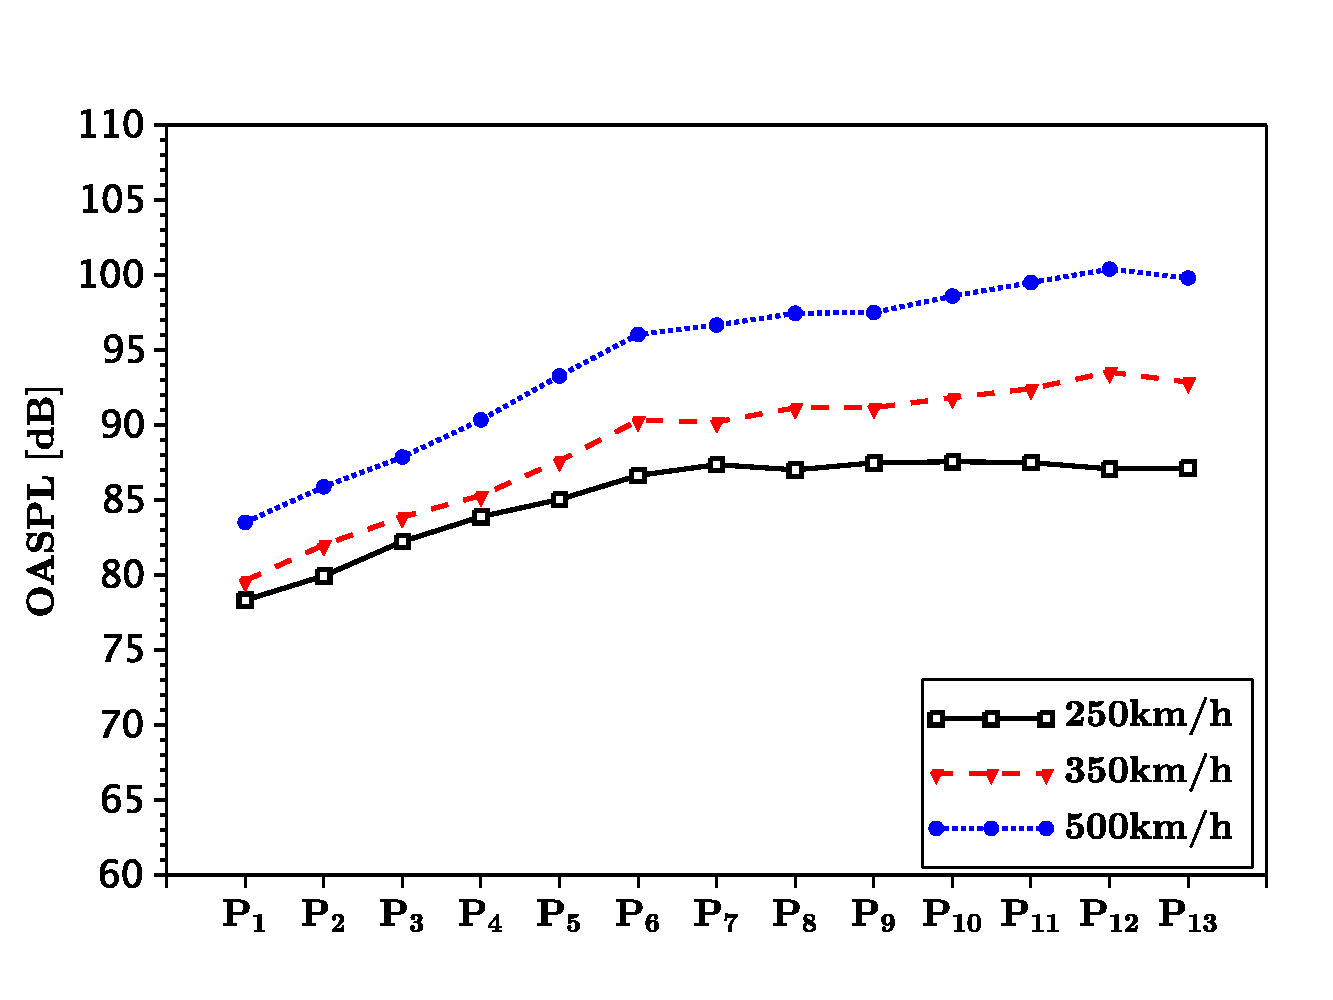
\includegraphics[width=0.55\textwidth]{Figures/oaspl_a.pdf}
  \neufigcaption{fig:ch0-cover}{外部图片插入样例}{Example of Including an External Image}
\end{figure}

\neufigref{fig:ch0-cover} 展示了通过 \verb|\includegraphics| 插入图片文件的方式。
正式论文中建议将图片统一放入 \texttt{Figures} 目录，并使用相对路径引用。

\subsection{PDF 或位图图片}
\begin{figure}[!htbp]
  \centering
  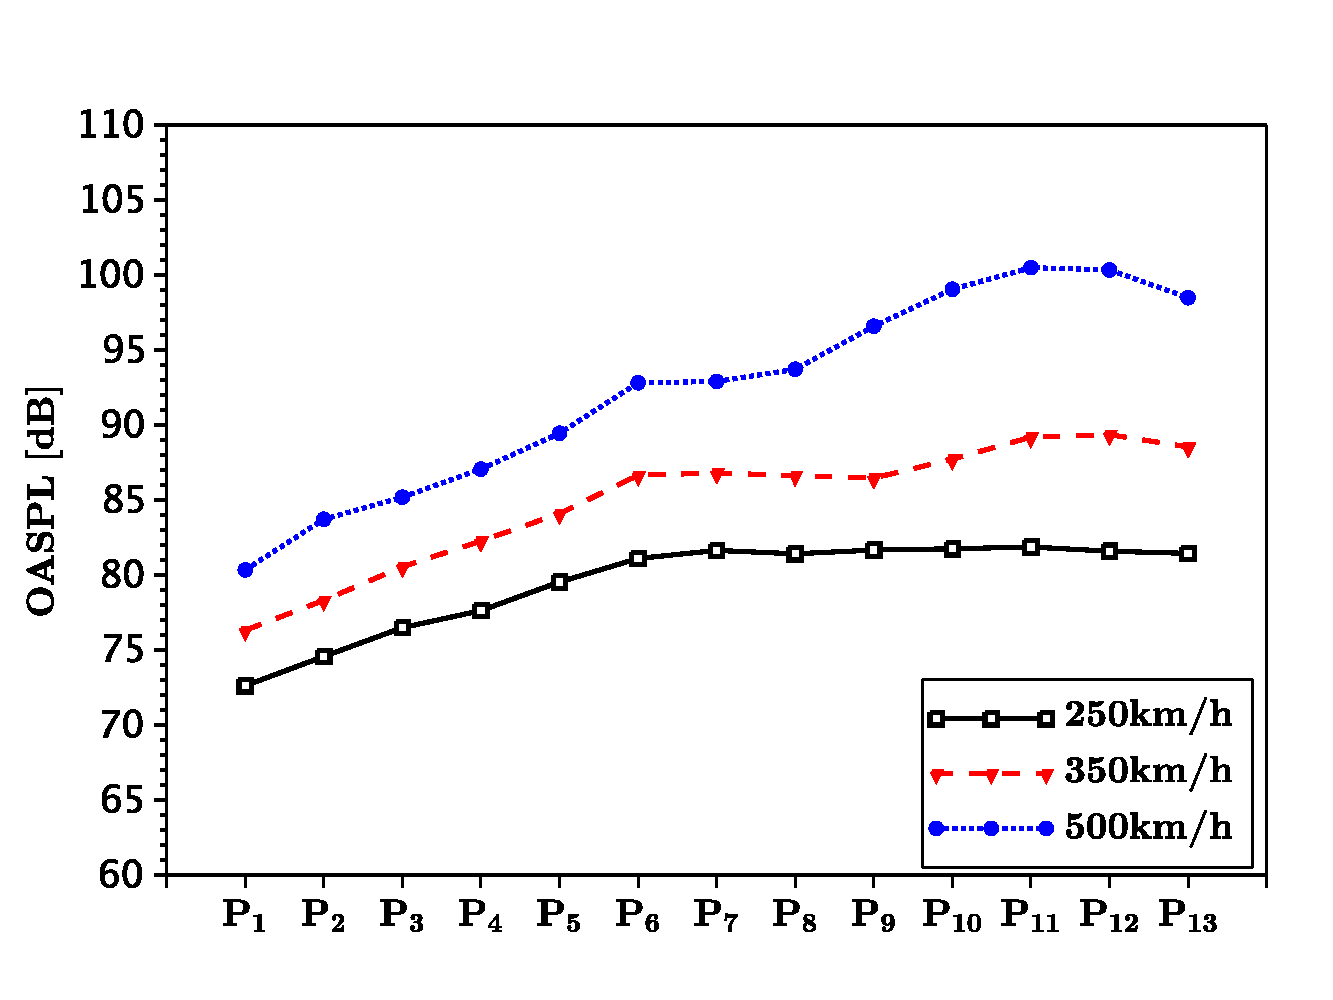
\includegraphics[width=0.55\textwidth]{Figures/oaspl_b.pdf}
  \neufigcaption{fig:ch0-pdf}{PDF 图片插入样例}{Example of Including a PDF Figure}
\end{figure}

PDF、PNG、JPG 等常见图片格式均可通过 \verb|\includegraphics| 插入。
若图片由绘图软件或数据分析程序导出，建议优先使用 PDF 格式以保持较清晰的显示效果。

\subsection{并列图片}
\begin{figure}[!htbp]
  \centering
  \begin{minipage}[t]{0.49\linewidth}
    \centering
    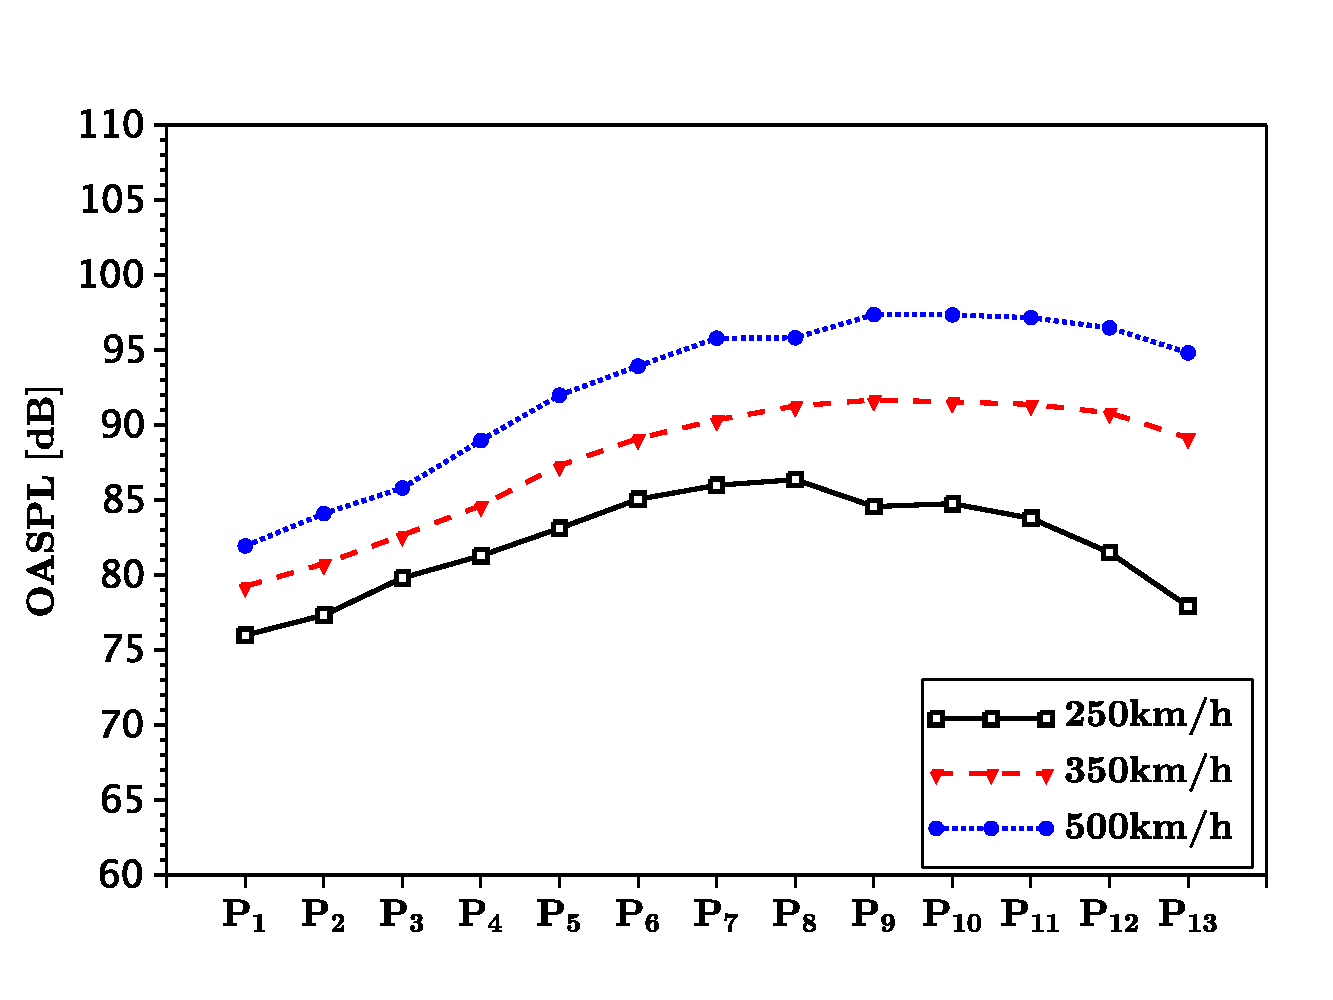
\includegraphics[width=\linewidth]{Figures/oaspl_c.pdf}
  \end{minipage}
  \hfill
  \begin{minipage}[t]{0.49\linewidth}
    \centering
    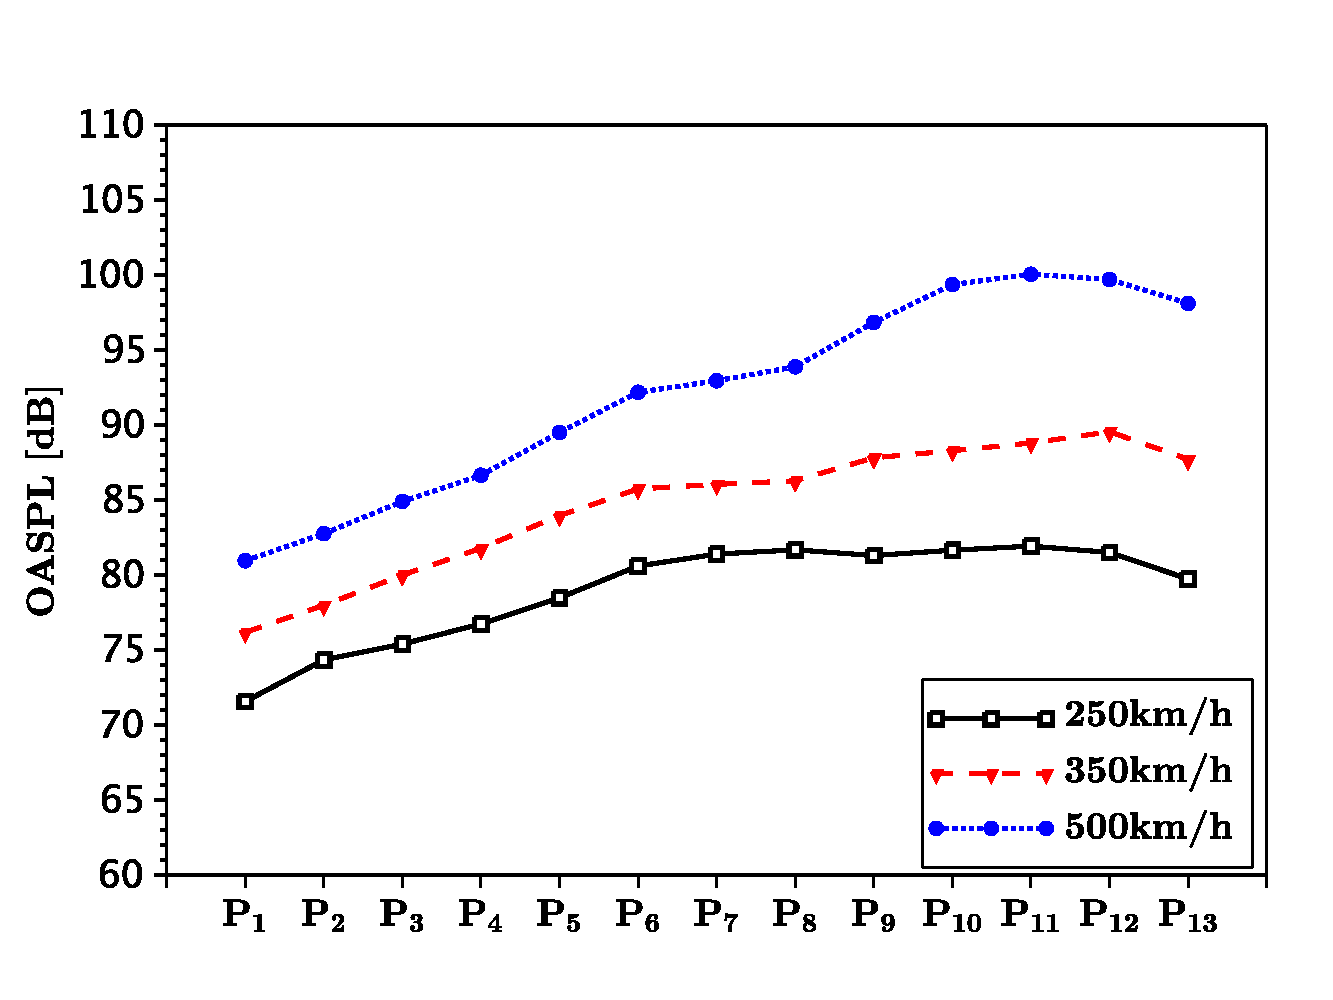
\includegraphics[width=\linewidth]{Figures/oaspl_d.pdf}
  \end{minipage}
  \neufigcaption{fig:ch0-side-by-side}{普通并列图形排版样例}{Example of Side-by-Side Figures}
\end{figure}

\neufigref{fig:ch0-side-by-side} 使用 \texttt{minipage} 完成普通并列排版。
当两幅图共享一个总标题且不需要分别引用时，可使用这种方式。

\subsection{并列子图}
\begin{figure}[!htbp]
  \centering
  \begin{neusubfigure}{0.49\linewidth}
    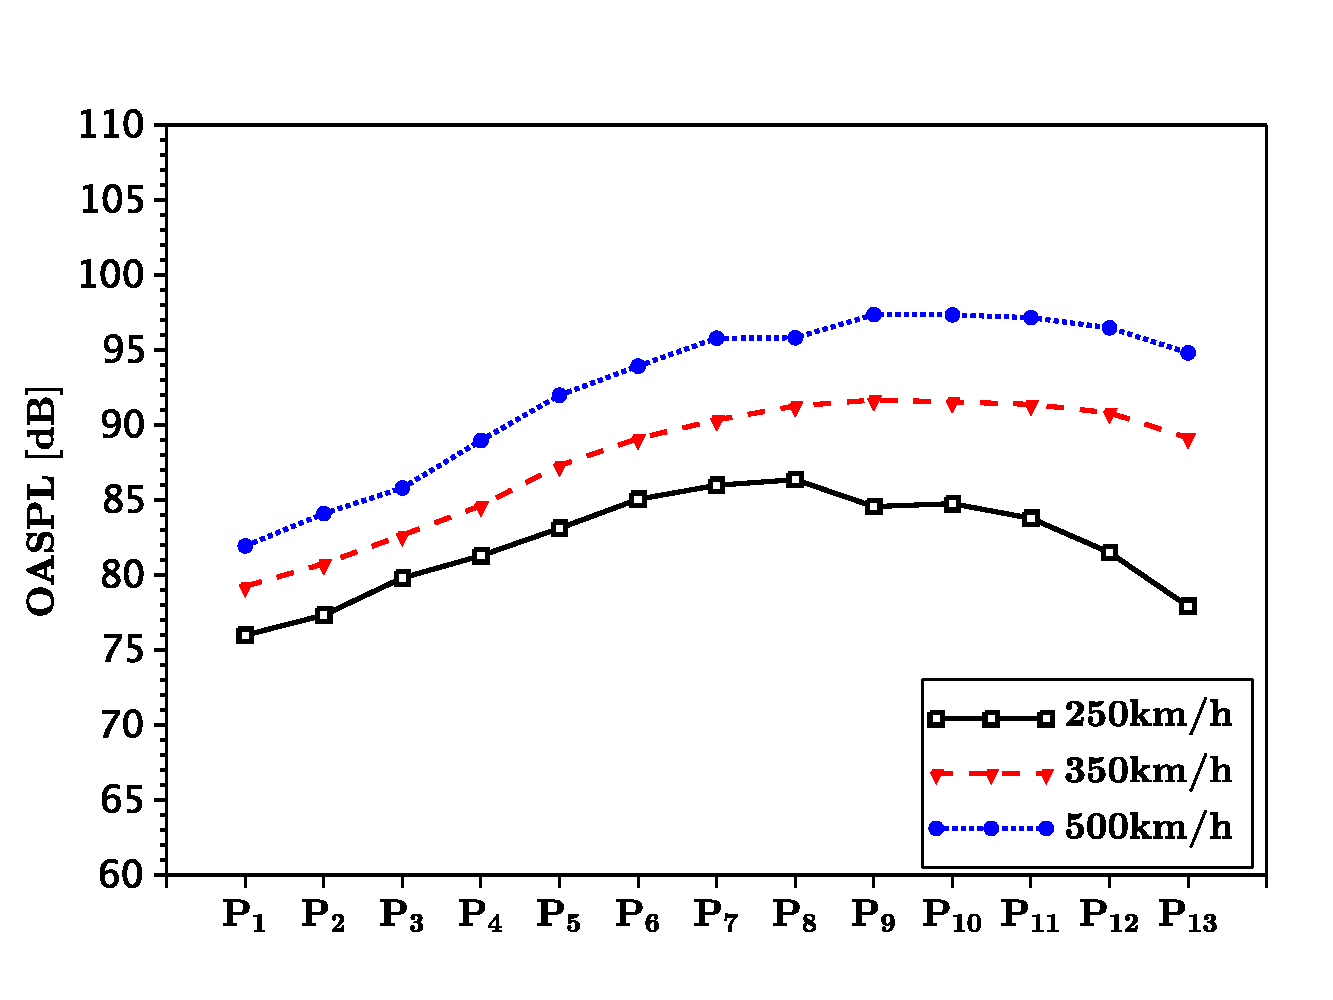
\includegraphics[width=\linewidth]{Figures/oaspl_c.pdf}
    \neusubfigcaption{fig:ch0-side-by-side-a}{工况一}
  \end{neusubfigure}
  \hfill
  \begin{neusubfigure}{0.49\linewidth}
    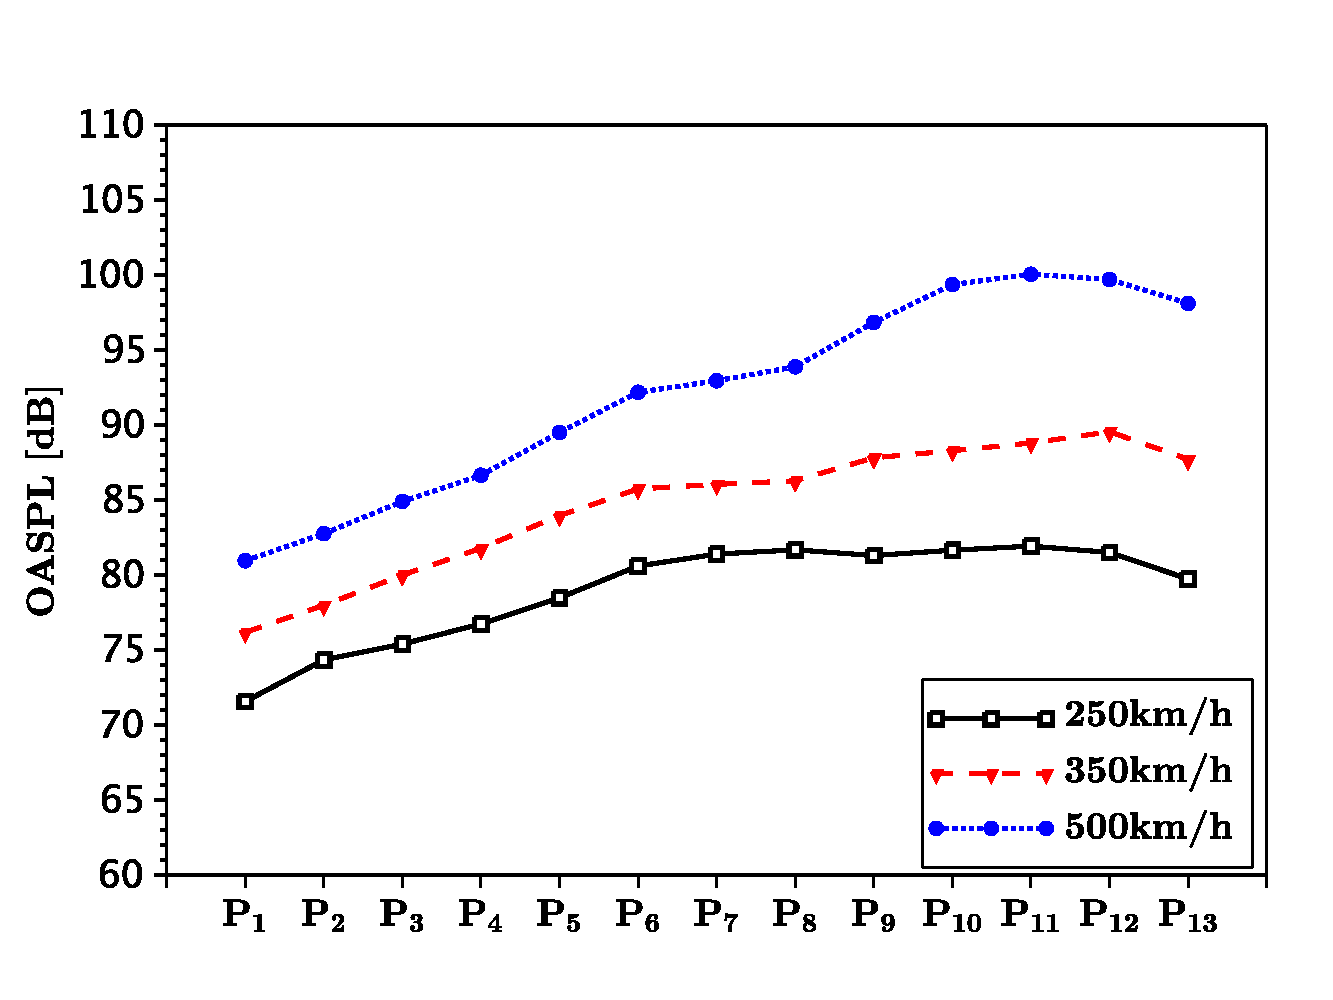
\includegraphics[width=\linewidth]{Figures/oaspl_d.pdf}
    \neusubfigcaption{fig:ch0-side-by-side-b}{工况二}
  \end{neusubfigure}
  \neufigcaption{fig:ch0-subfigures}{并列子图排版样例}{Example of Side-by-Side Subfigures}
\end{figure}

\neufigref{fig:ch0-subfigures} 使用 \texttt{neusubfigure} 完成并列子图排版。
其中 \neusubfigref{fig:ch0-side-by-side-a} 和 \neusubfigref{fig:ch0-side-by-side-b} 可分别引用到子图。
当两幅图共享一个总标题且需要分别引用时，可使用这种方式；如果每幅图需要完全独立的图号，建议拆成两个独立的 \texttt{figure} 环境。

\subsection{二乘二子图}
\begin{figure}[!htbp]
  \centering
  \begin{neusubfigure}{0.49\linewidth}
    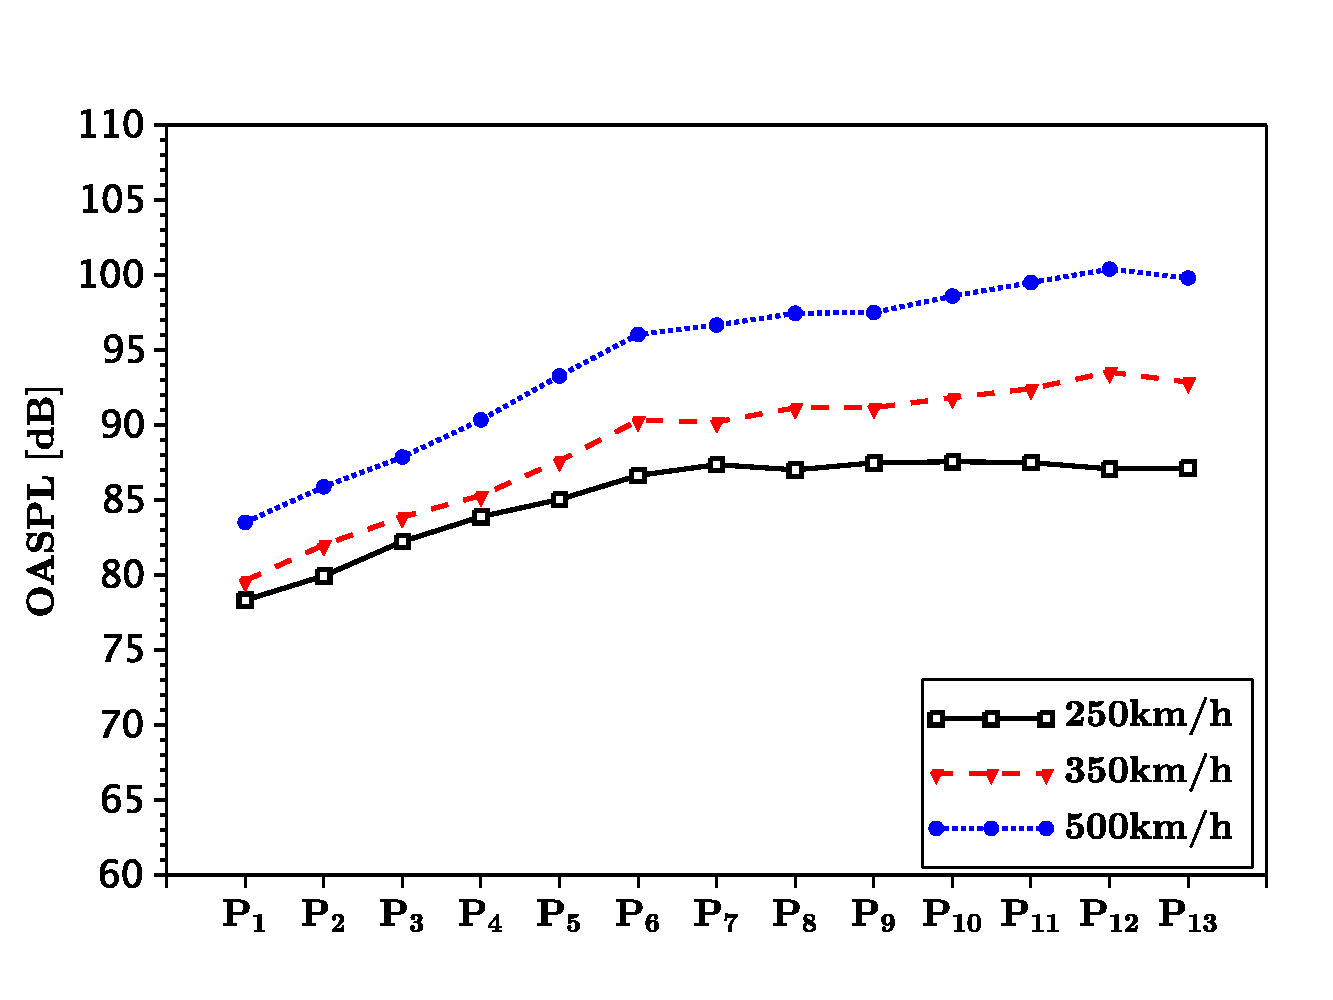
\includegraphics[width=\linewidth]{Figures/oaspl_a.pdf}
    \neusubfigcaption{fig:ch0-four-subfig-a}{工况一}
  \end{neusubfigure}
  \hfill
  \begin{neusubfigure}{0.49\linewidth}
    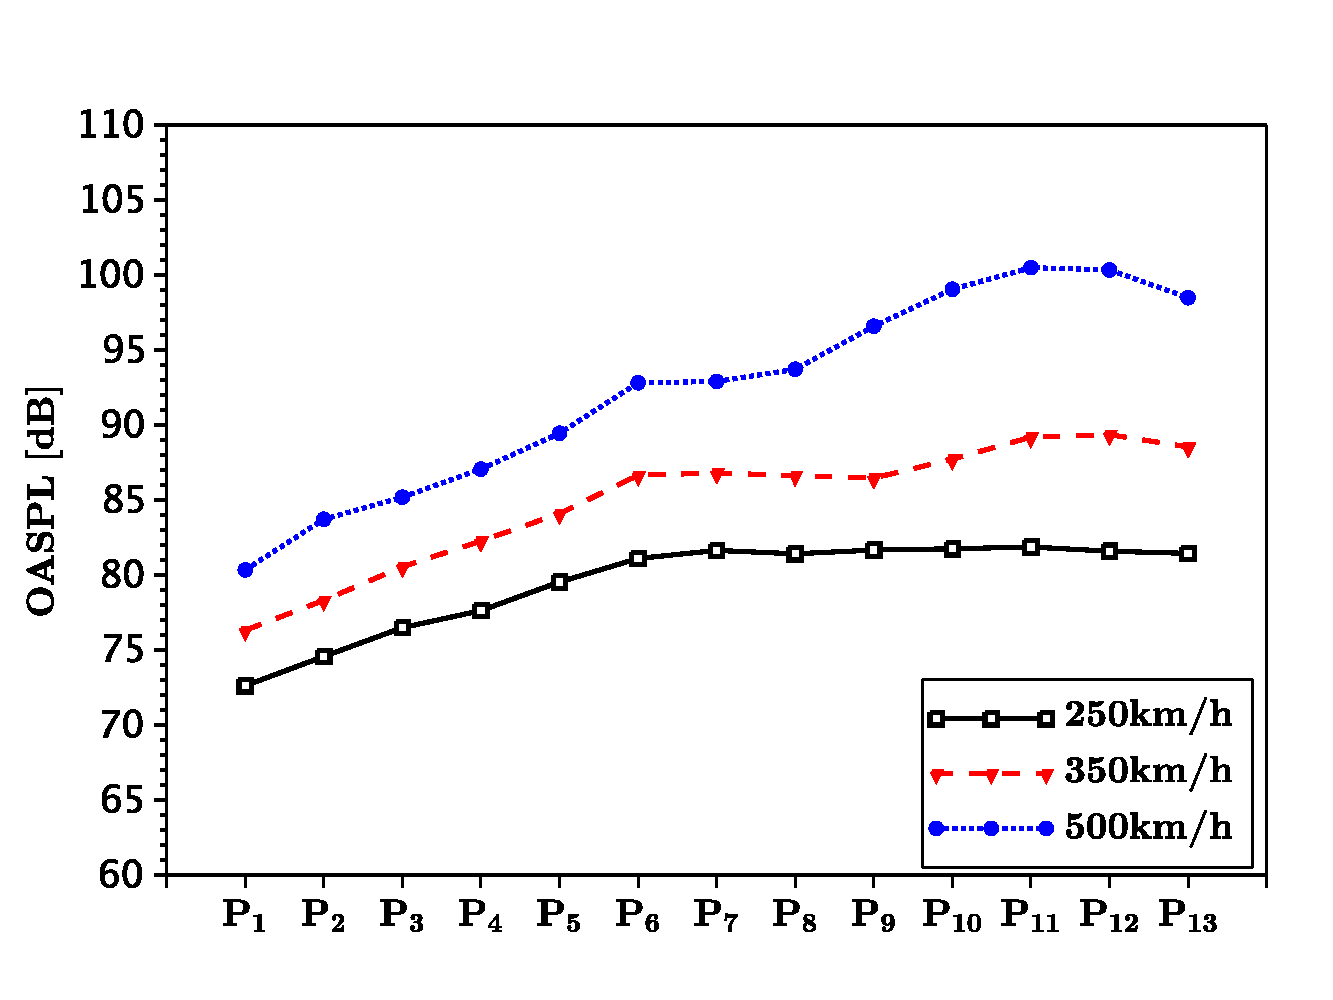
\includegraphics[width=\linewidth]{Figures/oaspl_b.pdf}
    \neusubfigcaption{fig:ch0-four-subfig-b}{工况二}
  \end{neusubfigure}
  \par\vspace{2bp}

  \begin{neusubfigure}{0.49\linewidth}
    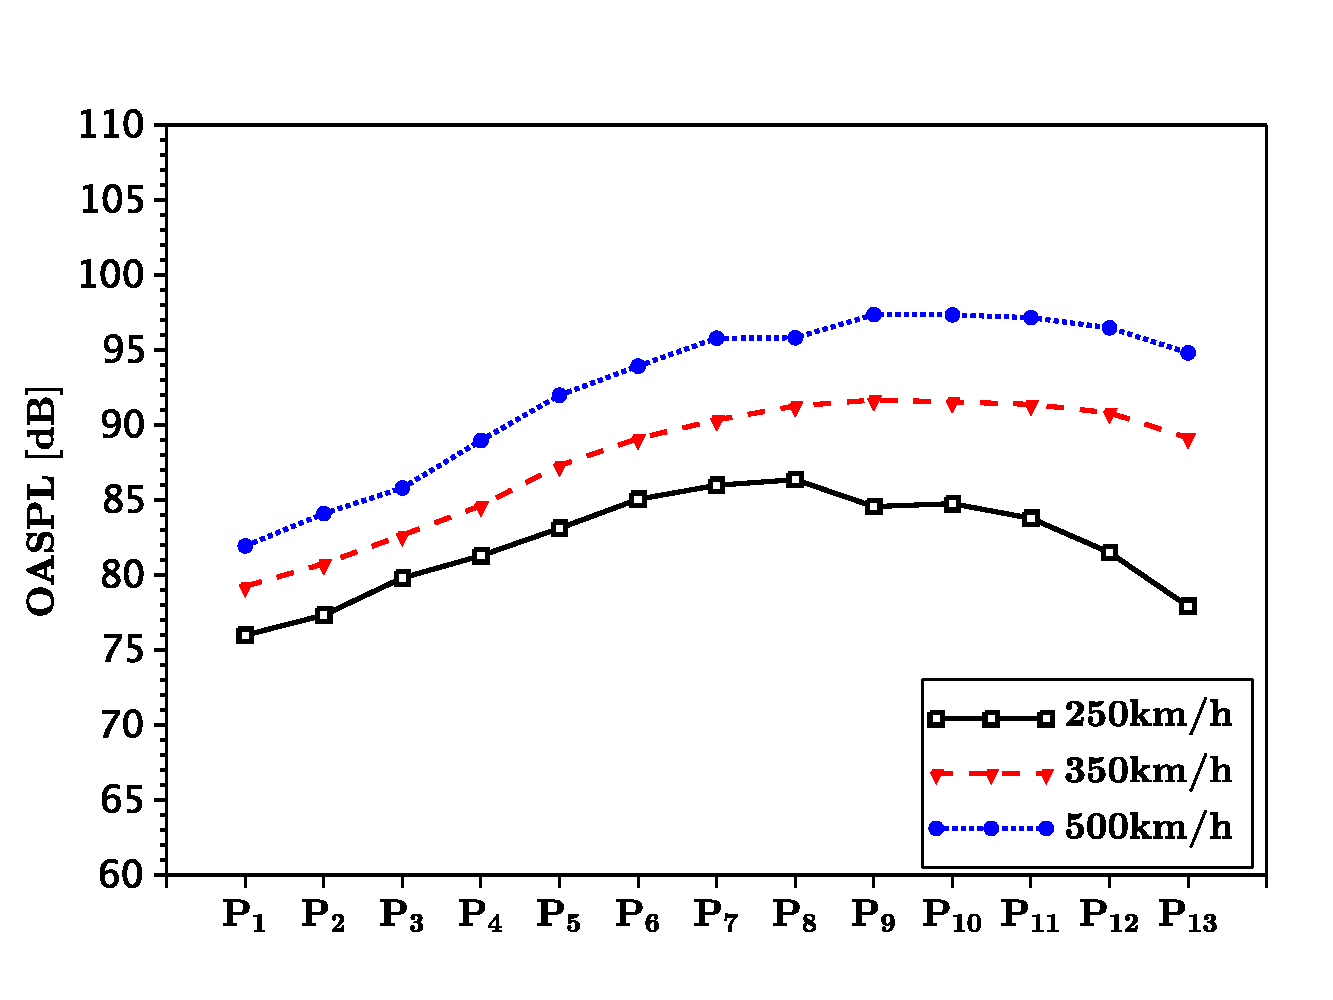
\includegraphics[width=\linewidth]{Figures/oaspl_c.pdf}
    \neusubfigcaption{fig:ch0-four-subfig-c}{工况三}
  \end{neusubfigure}
  \hfill
  \begin{neusubfigure}{0.49\linewidth}
    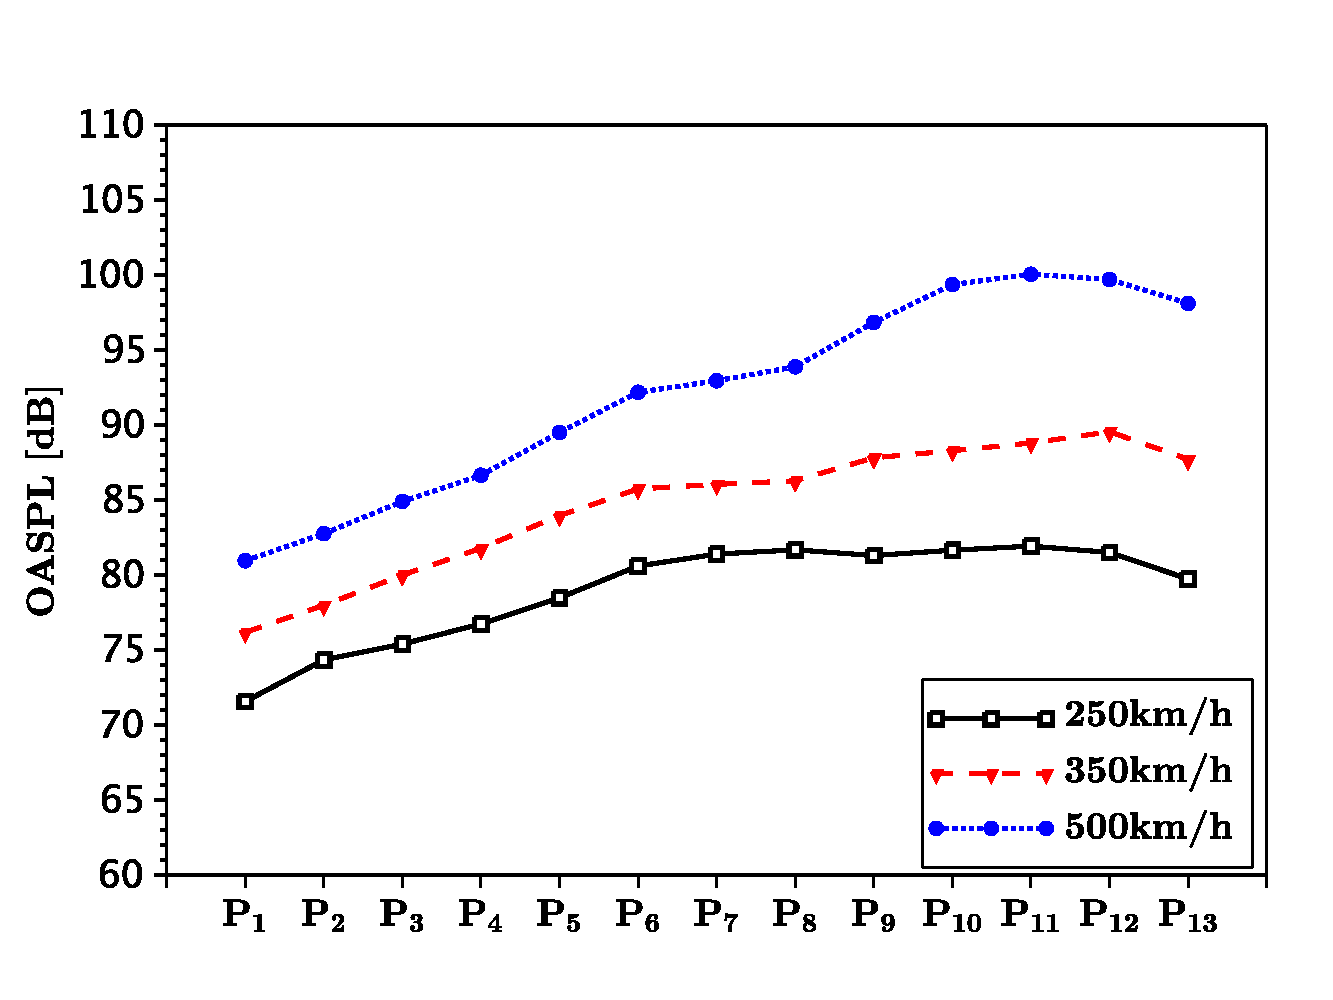
\includegraphics[width=\linewidth]{Figures/oaspl_d.pdf}
    \neusubfigcaption{fig:ch0-four-subfig-d}{工况四}
  \end{neusubfigure}
  \neufigcaption{fig:ch0-four-subfigures}{二乘二子图排版样例}{Example of Two-by-Two Subfigures}
\end{figure}

\neufigref{fig:ch0-four-subfigures} 展示了四幅子图的二乘二排布。
例如 \neusubfigref{fig:ch0-four-subfig-a} 至 \neusubfigref{fig:ch0-four-subfig-d} 可分别引用到四个子图。
排版时建议注意以下几点：
\begin{itemize}
  \item 子图宽度通常可取 \verb|0.48\linewidth| 至 \verb|0.49\linewidth|。
  \item 每行两个子图之间使用 \verb|\hfill| 自动拉开横向间距。
  \item 两行之间可用少量 \verb|\par\vspace| 控制垂直间距。
\end{itemize}

\section{表格排版}

本模板提供 \verb|\neutabcaption{label}{中文题名}{English title}| 用于生成中英文表题。
表题应置于表格上方，正文中使用 \verb|\neutabref{label}| 引用。
表格同样建议使用 \verb|[!htbp]|。如果表格过高导致页底空白，优先考虑缩小字号、调整列宽、拆分表格或使用跨页表格，而不是强制分页。

\subsection{三线表}

\begin{table}[!htbp]
  \centering
  \neutabcaption{tab:ch0-booktabs}{三线表样例}{Example of a Three-Line Table}
  \begin{tabular}{lccc}
    \toprule
    方法       & 准确率（\%）       & 召回率（\%）       & F1 值           \\
    \midrule
    Baseline & 85.2          & 84.1          & 0.846          \\
    Method A & 89.7          & 88.9          & 0.893          \\
    Proposed & \textbf{92.1} & \textbf{91.5} & \textbf{0.918} \\
    \bottomrule
  \end{tabular}
\end{table}

\neutabref{tab:ch0-booktabs} 展示了推荐的三线表格式。
论文中应尽量避免过多竖线，以保持表格简洁。

\subsection{复杂表格}
\begin{table}[!htbp]
  \centering
  \neutabcaption{tab:ch0-complex}{合并单元格与自动换行表格样例}{Example of Merged Cells and Auto-Wrapping Columns}
  \begin{tabularx}{\textwidth}{llXc}
    \toprule
    类别                  & 指标  & 说明                               & 是否必需 \\
    \midrule
    \multirow{2}{*}{图形} & 分辨率 & 位图图片应保证在最终 PDF 中清晰可辨。            & 是    \\
                        & 题名  & 图题使用中英文双语标题，并位于图片下方。             & 是    \\
    \midrule
    \multirow{2}{*}{表格} & 宽度  & 宽表格可使用 \texttt{tabularx} 自动分配列宽。 & 否    \\
                        & 表注  & 表内说明应简明，必要时可在正文中解释。              & 否    \\
    \bottomrule
  \end{tabularx}
\end{table}

\neutabref{tab:ch0-complex} 同时展示了 \verb|\multirow|、\verb|\makecell| 可配合使用的复杂表格场景。
若单元格内容较长，优先使用 \texttt{tabularx} 或 \texttt{p\{...\}} 列类型控制宽度。

\section{公式排版}

公式应使用标准数学环境，并通过 \verb|\label| 设置标签。
引用公式时建议使用模板提供的 \verb|\neueqref{label}|。

\subsection{单行公式}
以分类任务中的交叉熵损失为例，可写为
\begin{equation}
  \mathcal{L}(\theta)
  = - \frac{1}{N}\sum_{i=1}^{N}\sum_{k=1}^{K} y_{ik}\log p_{ik}
  \label{eq:ch0-loss}
\end{equation}

如 \neueqref{eq:ch0-loss} 所示，带编号公式适合放置正文中需要引用的重要定义。

\subsection{多行公式}
循环模型中的状态更新和输出计算可写为
\begin{align}
  h_t       & = \sigma(W_x x_t + W_h h_{t-1} + b), \label{eq:ch0-state} \\
  \hat{y}_t & = \operatorname{softmax}(W_o h_t). \label{eq:ch0-output}
\end{align}

\neueqref{eq:ch0-state} 和 \neueqref{eq:ch0-output} 展示了多行公式的编号方式。
如果多行推导只需要一个编号，可使用 \texttt{aligned} 放在 \texttt{equation} 环境内部。

\subsection{分段函数与矩阵}
分段函数和矩阵经常同时出现在数学定义中，例如
\begin{equation}
  g(x)=
  \begin{cases}
    0, & x < 0,       \\
    x, & 0 \le x < 1, \\
    1, & x \ge 1,
  \end{cases}
  \qquad
  A =
  \begin{bmatrix}
    1 & 0 & 0 \\
    0 & 1 & 0 \\
    0 & 0 & 1
  \end{bmatrix}.
  \label{eq:ch0-piecewise}
\end{equation}

\neueqref{eq:ch0-piecewise} 展示了分段函数和矩阵的常见写法。

\section{算法伪代码}

计算机类论文常需要给出算法步骤。本文档在 \texttt{main.tex} 中加载了 \texttt{algorithm} 和 \texttt{algorithmic} 宏包，可以直接使用如下环境。

\begin{algorithm}[!htbp]
  \caption{样例训练流程}
  \label{alg:ch0-training}
  \begin{algorithmic}[1]
    \REQUIRE Training set $\mathcal{D}$, learning rate $\eta$, maximum epoch $T$
    \ENSURE Model parameters $\theta$
    \STATE Initialize parameters $\theta$
    \FOR{$t = 1$ to $T$}
    \STATE Sample a mini-batch $\mathcal{B}$ from $\mathcal{D}$
    \STATE Compute loss $\mathcal{L}(\theta)$ by \neueqref{eq:ch0-loss}
    \STATE Update $\theta \leftarrow \theta - \eta \nabla_{\theta}\mathcal{L}(\theta)$
    \ENDFOR
    \RETURN $\theta$
  \end{algorithmic}
\end{algorithm}

算法~\ref{alg:ch0-training} 展示了带行号的伪代码。
若需要中文关键字，可在导言区重定义相应命令。

\section{引用、链接与交叉引用}

参考文献引用可使用两种模板命令：
\begin{itemize}
  \item 上标引用使用 \verb|\upcite{key}|，适合放在句末，例如已有研究讨论了神经网络轻量化问题\upcite{guo_2023_research}。
  \item 正文引用使用 \verb|\inlinecite{key}|，适合作为句子成分，例如文献 \inlinecite{thakkar_2018_performance} 给出了系统性能评测案例。
\end{itemize}
多篇文献可写在同一条引用命令中，例如区块链平台相关研究\upcite{zheng_2019_nutbaas,thakkar_2018_performance}。

交叉引用建议统一使用模板命令：
\begin{itemize}
  \item 图引用：\verb|\neufigref{fig:ch0-pdf}|，效果为 \neufigref{fig:ch0-pdf}。
  \item 子图引用：\verb|\neusubfigref{fig:ch0-four-subfig-a}|，效果为 \neusubfigref{fig:ch0-four-subfig-a}。
  \item 表引用：\verb|\neutabref{tab:ch0-complex}|，效果为 \neutabref{tab:ch0-complex}。
  \item 公式引用：\verb|\neueqref{eq:ch0-loss}|，效果为 \neueqref{eq:ch0-loss}。
  \item 算法引用：当前模板未单独封装算法引用命令，可写作“算法~\ref{alg:ch0-training}”。
\end{itemize}
模板提供的公开命令和环境可参考 \texttt{README.md} 中的“模板命令说明”一节。
|，并从第~\ref{chap:introduction}~章开始组织正式内容。

\section{章节层级与正文段落}

论文正文通常从一级标题开始组织内容，一级标题使用 \verb|\chapter|，二级标题使用 \verb|\section|，三级标题使用 \verb|\subsection|。
本模板会自动设置章标题、节标题、页眉、页码和目录格式，作者只需要关注正文内容。
正文段落首行缩进、行距和中英文字体均由模板统一控制，一般不需要在正文中手动设置字号、字体或段间距。

中文正文可以直接书写；英文术语建议在首次出现时给出全称，例如自然语言处理（Natural Language Processing, NLP）。
行内公式可以写作 $E=mc^2$，行内代码或命令可以使用 \verb|\verb|，例如 \verb|%!TEX root = ./main.tex
\chapter{论文格式样例与模板验证}

本章作为模板的集中样例章，用于快速检查正文中常见排版元素的显示效果。
样例覆盖章节层级、正文段落、列表、脚注、图、表、公式、算法、交叉引用和参考文献引用等内容。
编写正式论文时，可以保留本章作为排版对照；定稿前可在 \texttt{main.tex} 中删除或注释 \verb|%!TEX root = ./main.tex
\chapter{论文格式样例与模板验证}

本章作为模板的集中样例章，用于快速检查正文中常见排版元素的显示效果。
样例覆盖章节层级、正文段落、列表、脚注、图、表、公式、算法、交叉引用和参考文献引用等内容。
编写正式论文时，可以保留本章作为排版对照；定稿前可在 \texttt{main.tex} 中删除或注释 \verb|%!TEX root = ./main.tex
\chapter{论文格式样例与模板验证}

本章作为模板的集中样例章，用于快速检查正文中常见排版元素的显示效果。
样例覆盖章节层级、正文段落、列表、脚注、图、表、公式、算法、交叉引用和参考文献引用等内容。
编写正式论文时，可以保留本章作为排版对照；定稿前可在 \texttt{main.tex} 中删除或注释 \verb|\input{chapter0-guide}|，并从第~\ref{chap:introduction}~章开始组织正式内容。

\section{章节层级与正文段落}

论文正文通常从一级标题开始组织内容，一级标题使用 \verb|\chapter|，二级标题使用 \verb|\section|，三级标题使用 \verb|\subsection|。
本模板会自动设置章标题、节标题、页眉、页码和目录格式，作者只需要关注正文内容。
正文段落首行缩进、行距和中英文字体均由模板统一控制，一般不需要在正文中手动设置字号、字体或段间距。

中文正文可以直接书写；英文术语建议在首次出现时给出全称，例如自然语言处理（Natural Language Processing, NLP）。
行内公式可以写作 $E=mc^2$，行内代码或命令可以使用 \verb|\verb|，例如 \verb|\input{chapter0-guide}|。
脚注示例如此处所示\footnote{脚注用于补充说明，不宜放置过长的正文内容。}。
若某页因图表浮动或分页规则没有排满，脚注可能跟随正文排版区而显得略高，这是正常的 LaTeX 页面构建结果。

\subsection{字体、字号与强调}

模板预定义了常用中文字体命令。正式论文中通常不需要手动切换字体；只有在展示样式、术语强调或特殊说明时才建议使用。
当前模板已经为默认宋体和 \verb|\song| 字族配置伪粗体，因此 \verb|\textbf| 或 \verb|\bfseries| 可以用于中文局部强调。
需要注意的是，中文加粗应克制使用；标题层级、术语定义或表格重点值可以适当加粗，大段正文不建议整体加粗。
如果需要更明显的标题式强调，可使用黑体或调整标题层级；如果只是普通正文重点，优先使用 \verb|\textbf|。

\begin{table}[!htbp]
  \centering
  \neutabcaption{tab:ch0-fonts}{字体与强调样例}{Examples of Fonts and Emphasis}
  \begin{tabular}{lll}
    \toprule
    命令             & 显示效果                         & 使用建议       \\
    \midrule
    \verb|\song|   & {\song 宋体文字示例}               & 正文默认字体     \\
    \verb|\textbf| & \textbf{加粗文字示例}              & 局部强调、表格重点值 \\
    \verb|\hei|    & {\hei 黑体文字示例}                & 标题或较强强调场景  \\
    \verb|\kai|    & {\kai 楷体文字示例}                & 摘要、题签或引用语  \\
    \verb|\fs|     & {\fs 仿宋文字示例}                 & 特殊文书类内容    \\
    \verb|\textit| & \textit{Italic text example} & 英文斜体或变量说明  \\
    \bottomrule
  \end{tabular}
\end{table}

\subsection{列表环境}

无序列表适合列出并列事项：
\begin{itemize}
  \item 图题位于图下方，表题位于表上方。
  \item 图表应使用中英文双语标题。
  \item 公式、图、表、算法均应使用标签进行交叉引用。
\end{itemize}

有序列表适合描述步骤：
\begin{enumerate}
  \item 在 \texttt{main.tex} 中填写论文元信息。
  \item 在各章文件中撰写正文内容。
  \item 使用 \texttt{latexmk -xelatex main.tex} 完成编译。
\end{enumerate}

\section{图形排版}

本模板提供 \verb|\neufigcaption{label}{中文题名}{English title}| 用于生成中英文图题。
图题应置于图形下方，正文中使用 \verb|\neufigref{label}| 引用。
图形建议使用 \verb|[!htbp]| 浮动参数，让 LaTeX 在当前位置、页顶、页底或浮动页中选择较合适的位置；除非必须固定位置，否则不建议使用 \verb|[H]|。

\subsection{外部图片}
\begin{figure}[!htbp]
  \centering
  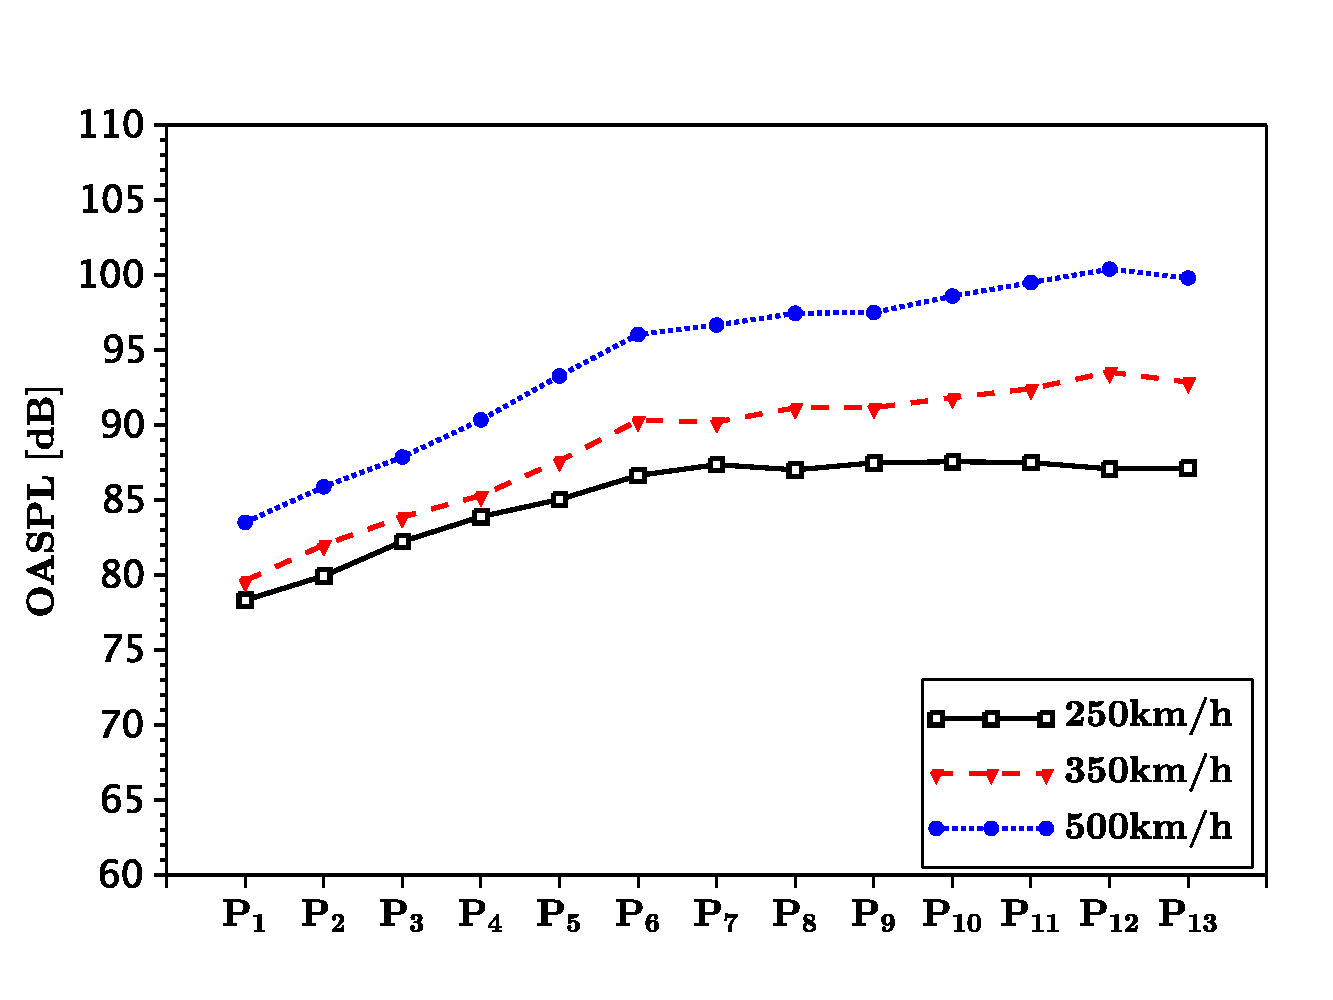
\includegraphics[width=0.55\textwidth]{Figures/oaspl_a.pdf}
  \neufigcaption{fig:ch0-cover}{外部图片插入样例}{Example of Including an External Image}
\end{figure}

\neufigref{fig:ch0-cover} 展示了通过 \verb|\includegraphics| 插入图片文件的方式。
正式论文中建议将图片统一放入 \texttt{Figures} 目录，并使用相对路径引用。

\subsection{PDF 或位图图片}
\begin{figure}[!htbp]
  \centering
  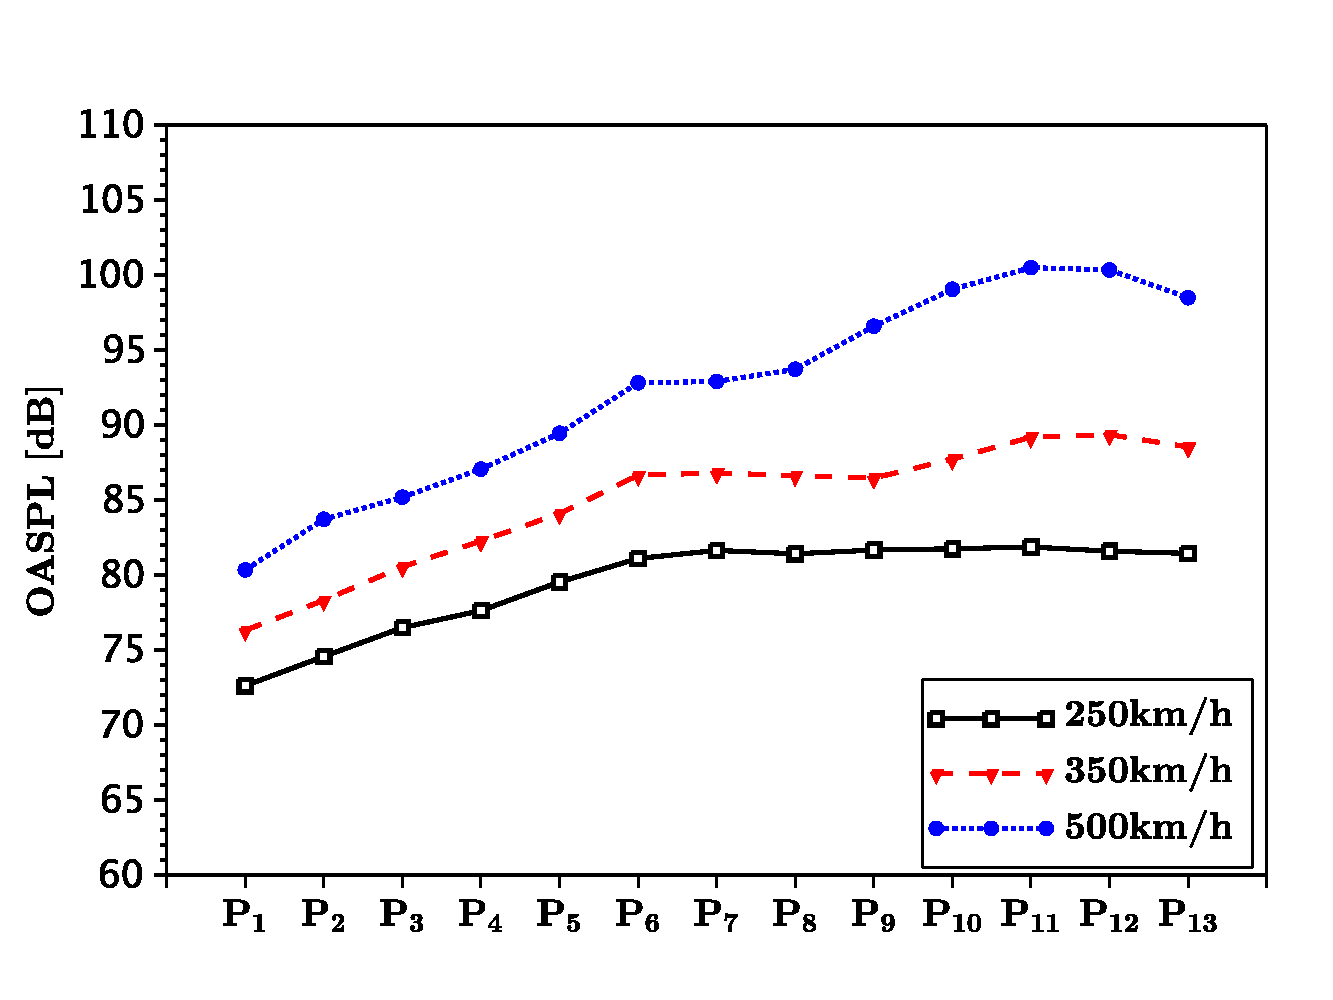
\includegraphics[width=0.55\textwidth]{Figures/oaspl_b.pdf}
  \neufigcaption{fig:ch0-pdf}{PDF 图片插入样例}{Example of Including a PDF Figure}
\end{figure}

PDF、PNG、JPG 等常见图片格式均可通过 \verb|\includegraphics| 插入。
若图片由绘图软件或数据分析程序导出，建议优先使用 PDF 格式以保持较清晰的显示效果。

\subsection{并列图片}
\begin{figure}[!htbp]
  \centering
  \begin{minipage}[t]{0.49\linewidth}
    \centering
    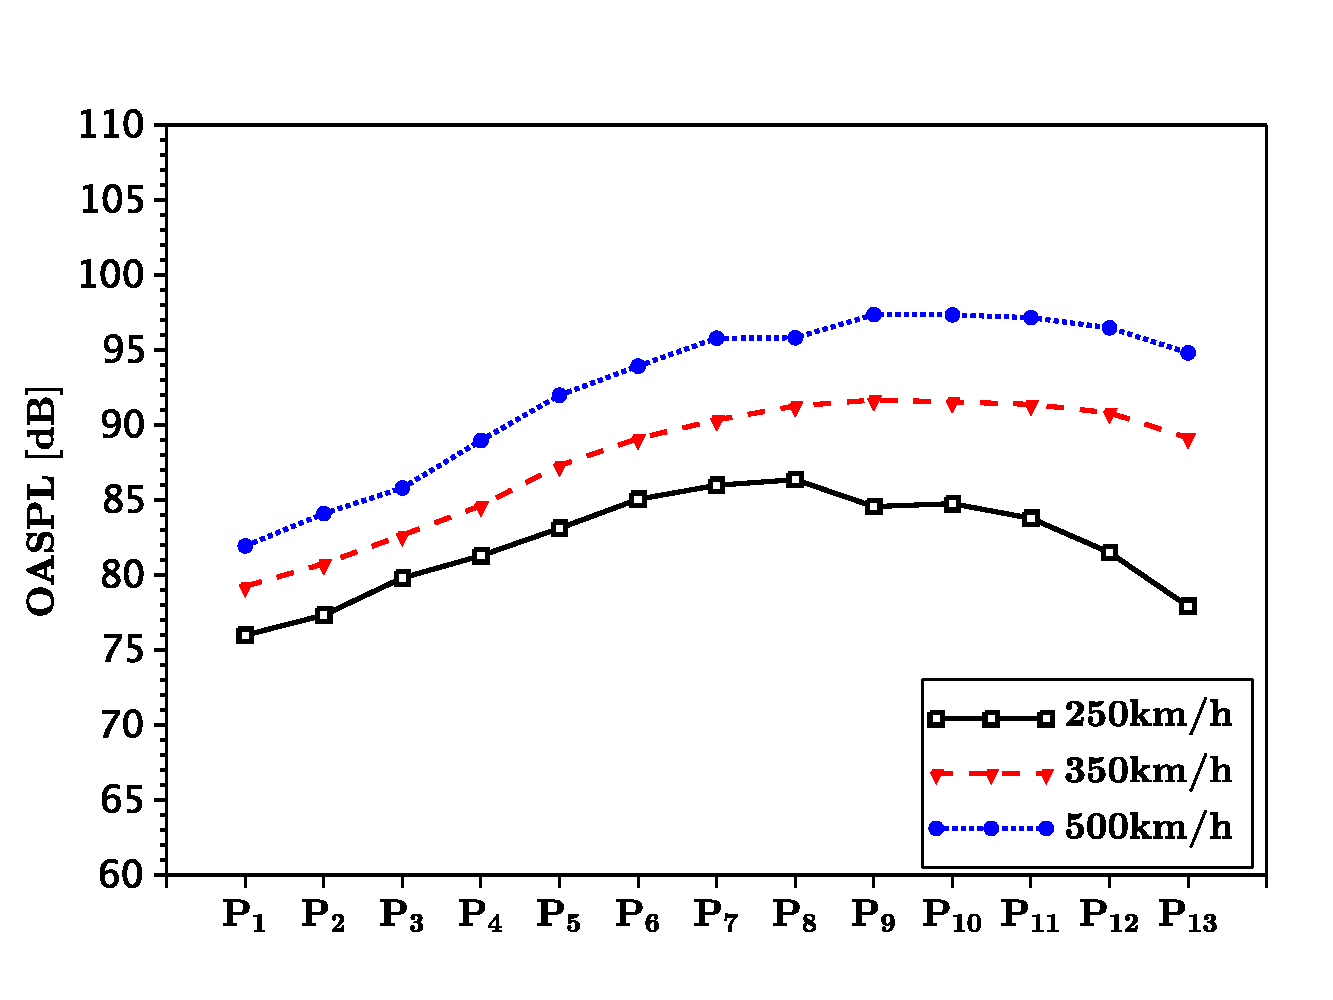
\includegraphics[width=\linewidth]{Figures/oaspl_c.pdf}
  \end{minipage}
  \hfill
  \begin{minipage}[t]{0.49\linewidth}
    \centering
    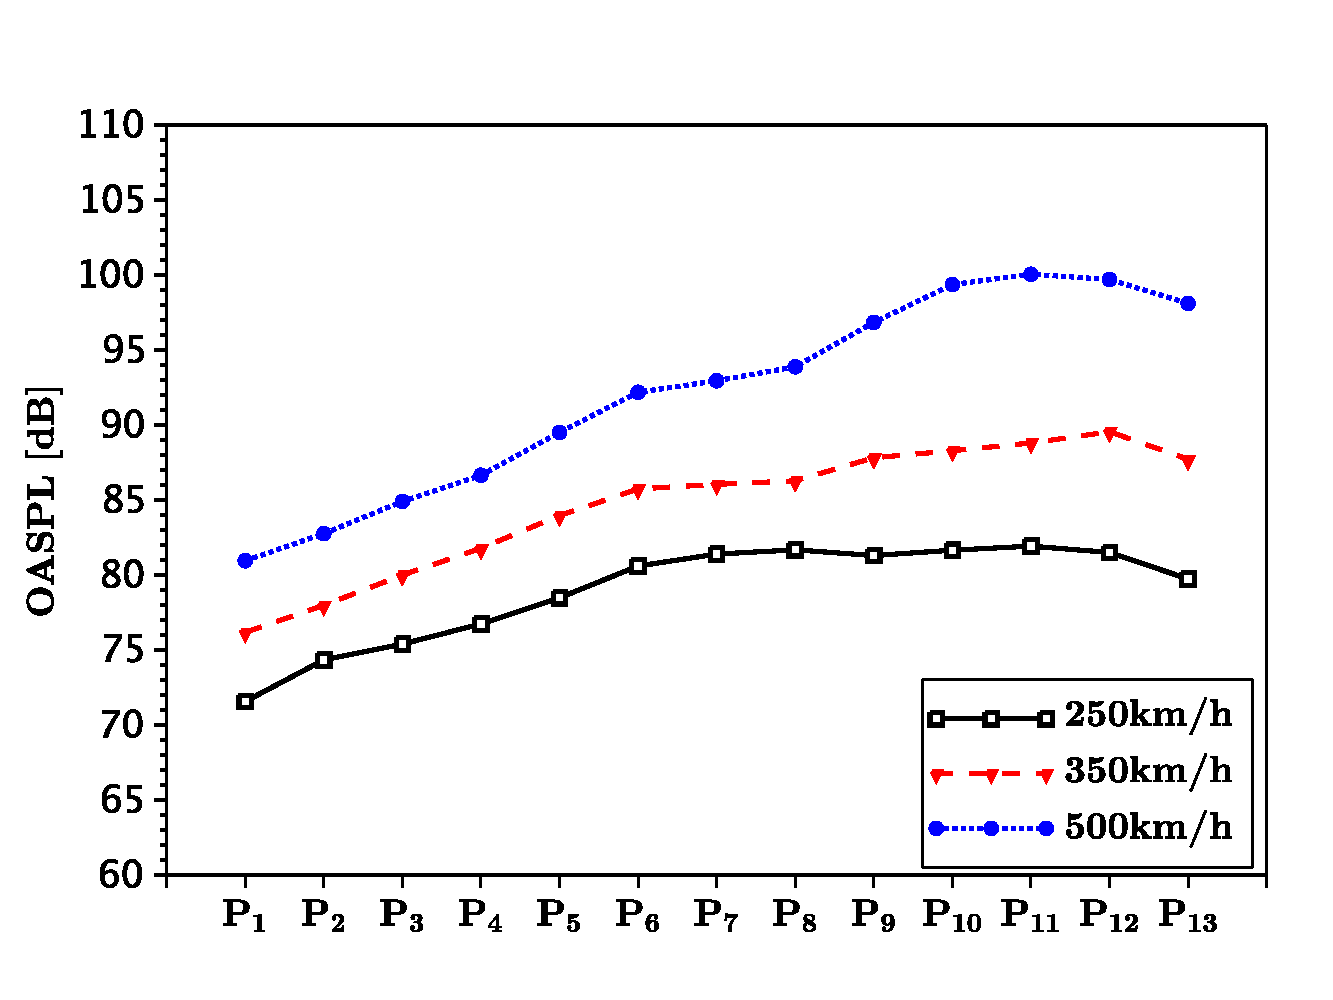
\includegraphics[width=\linewidth]{Figures/oaspl_d.pdf}
  \end{minipage}
  \neufigcaption{fig:ch0-side-by-side}{普通并列图形排版样例}{Example of Side-by-Side Figures}
\end{figure}

\neufigref{fig:ch0-side-by-side} 使用 \texttt{minipage} 完成普通并列排版。
当两幅图共享一个总标题且不需要分别引用时，可使用这种方式。

\subsection{并列子图}
\begin{figure}[!htbp]
  \centering
  \begin{neusubfigure}{0.49\linewidth}
    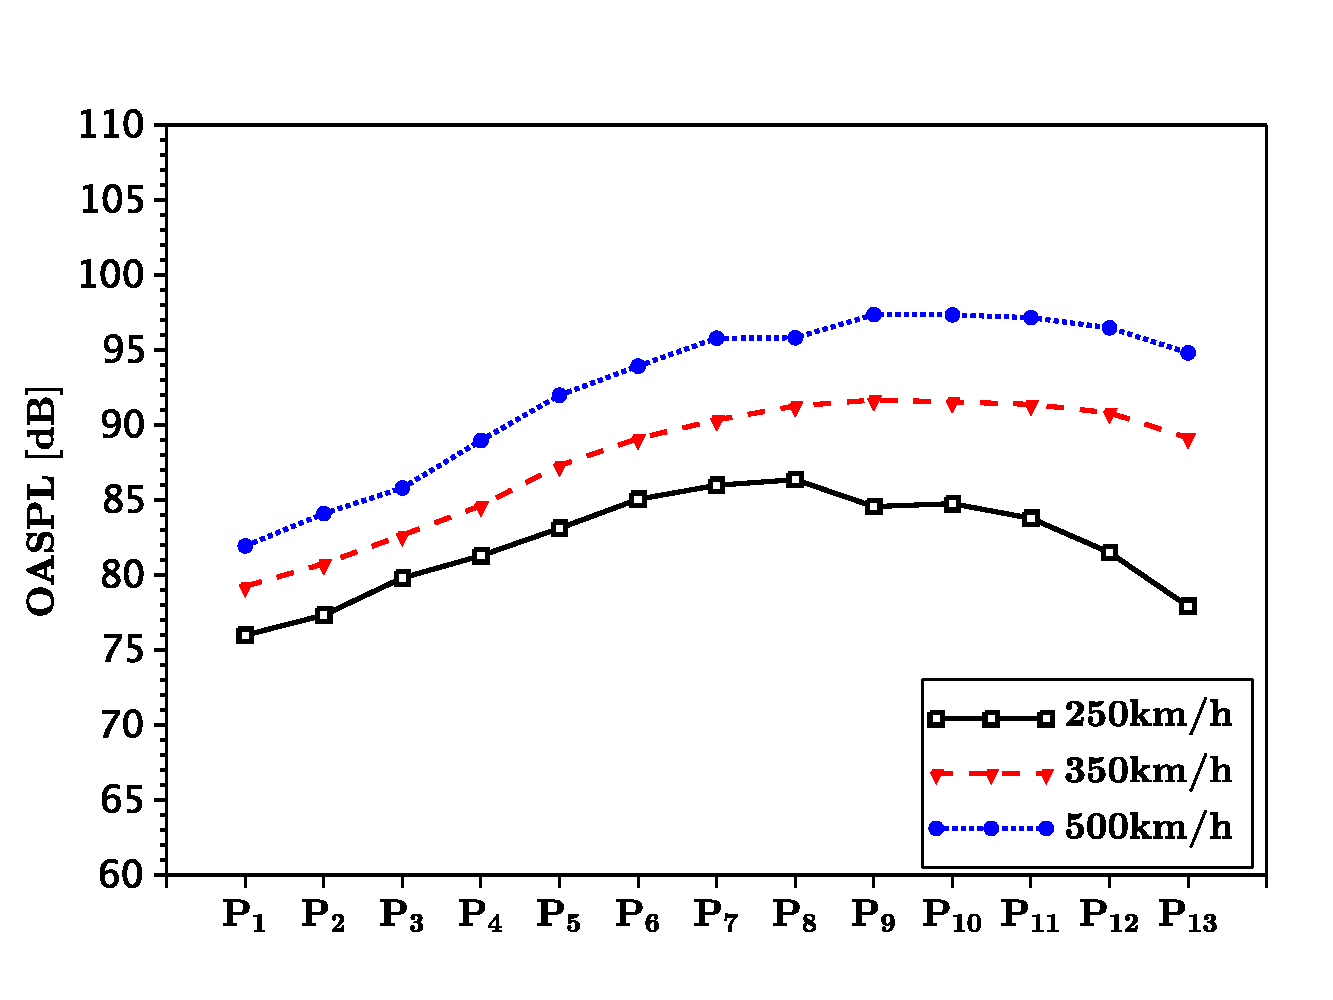
\includegraphics[width=\linewidth]{Figures/oaspl_c.pdf}
    \neusubfigcaption{fig:ch0-side-by-side-a}{工况一}
  \end{neusubfigure}
  \hfill
  \begin{neusubfigure}{0.49\linewidth}
    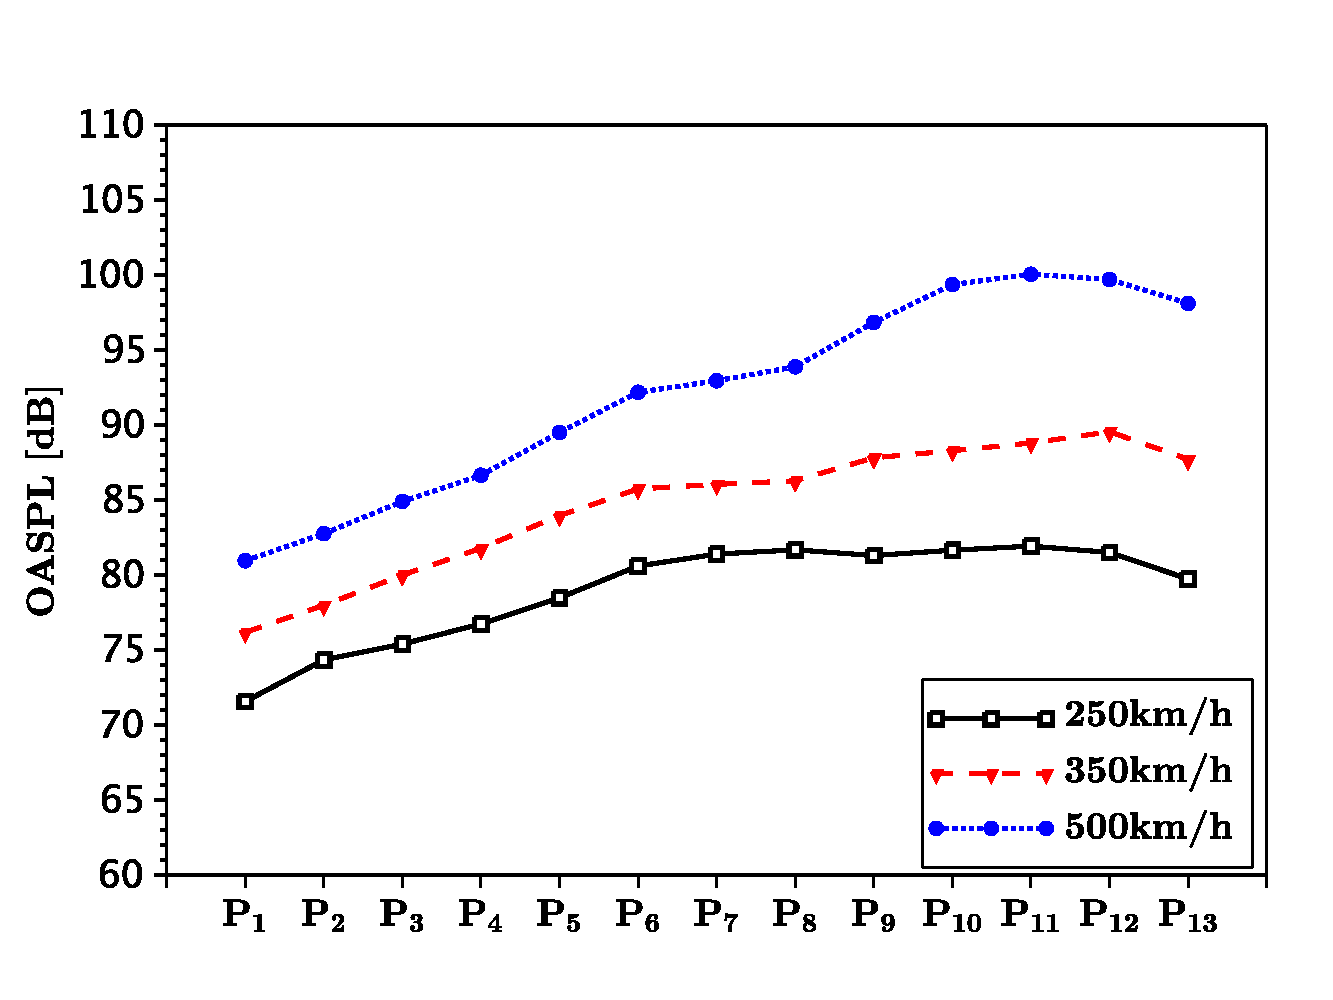
\includegraphics[width=\linewidth]{Figures/oaspl_d.pdf}
    \neusubfigcaption{fig:ch0-side-by-side-b}{工况二}
  \end{neusubfigure}
  \neufigcaption{fig:ch0-subfigures}{并列子图排版样例}{Example of Side-by-Side Subfigures}
\end{figure}

\neufigref{fig:ch0-subfigures} 使用 \texttt{neusubfigure} 完成并列子图排版。
其中 \neusubfigref{fig:ch0-side-by-side-a} 和 \neusubfigref{fig:ch0-side-by-side-b} 可分别引用到子图。
当两幅图共享一个总标题且需要分别引用时，可使用这种方式；如果每幅图需要完全独立的图号，建议拆成两个独立的 \texttt{figure} 环境。

\subsection{二乘二子图}
\begin{figure}[!htbp]
  \centering
  \begin{neusubfigure}{0.49\linewidth}
    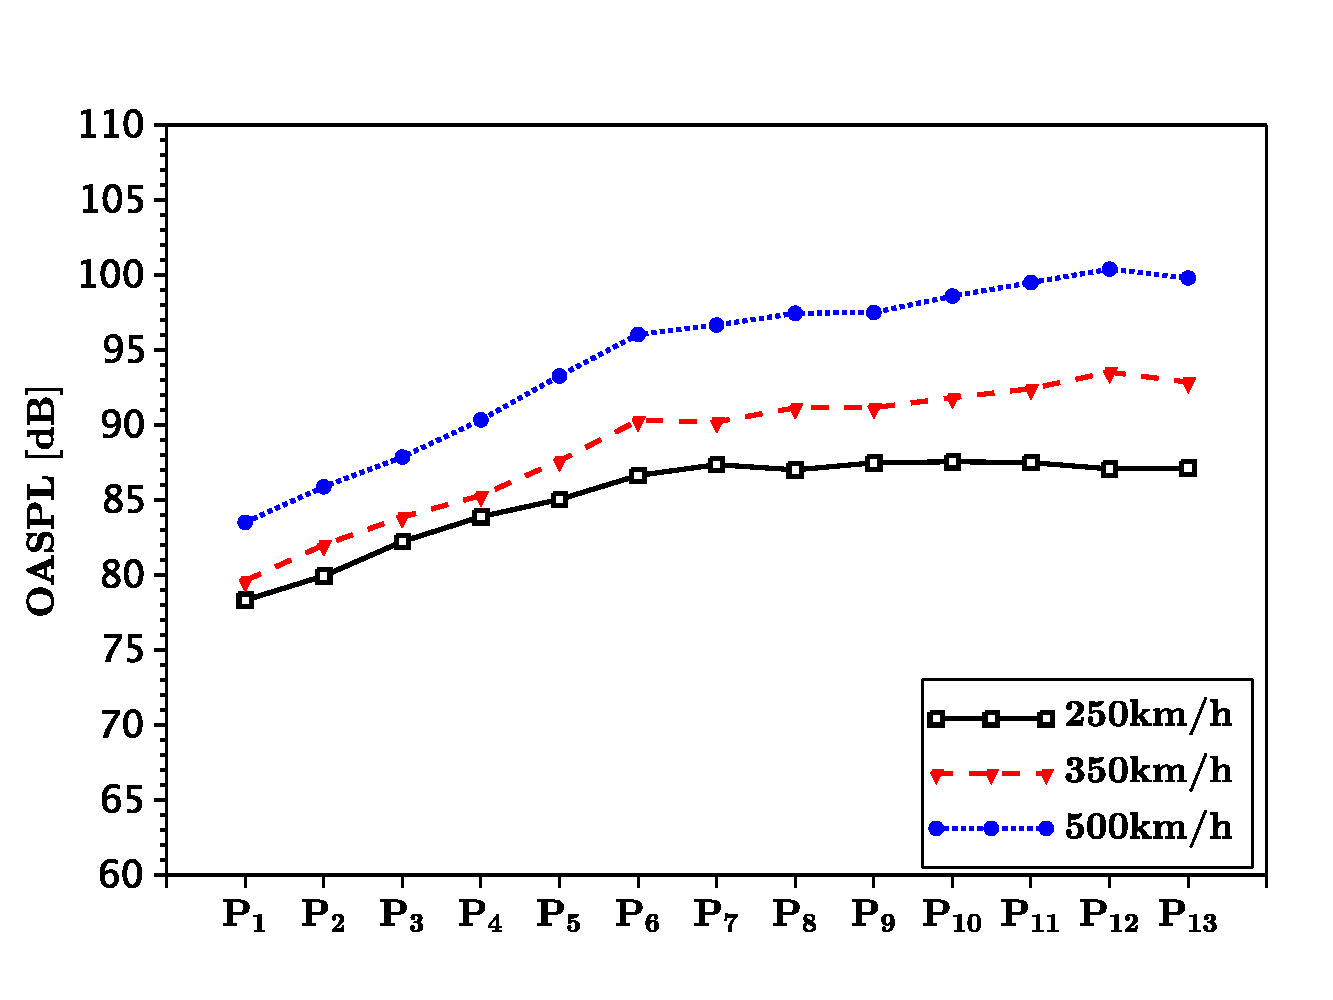
\includegraphics[width=\linewidth]{Figures/oaspl_a.pdf}
    \neusubfigcaption{fig:ch0-four-subfig-a}{工况一}
  \end{neusubfigure}
  \hfill
  \begin{neusubfigure}{0.49\linewidth}
    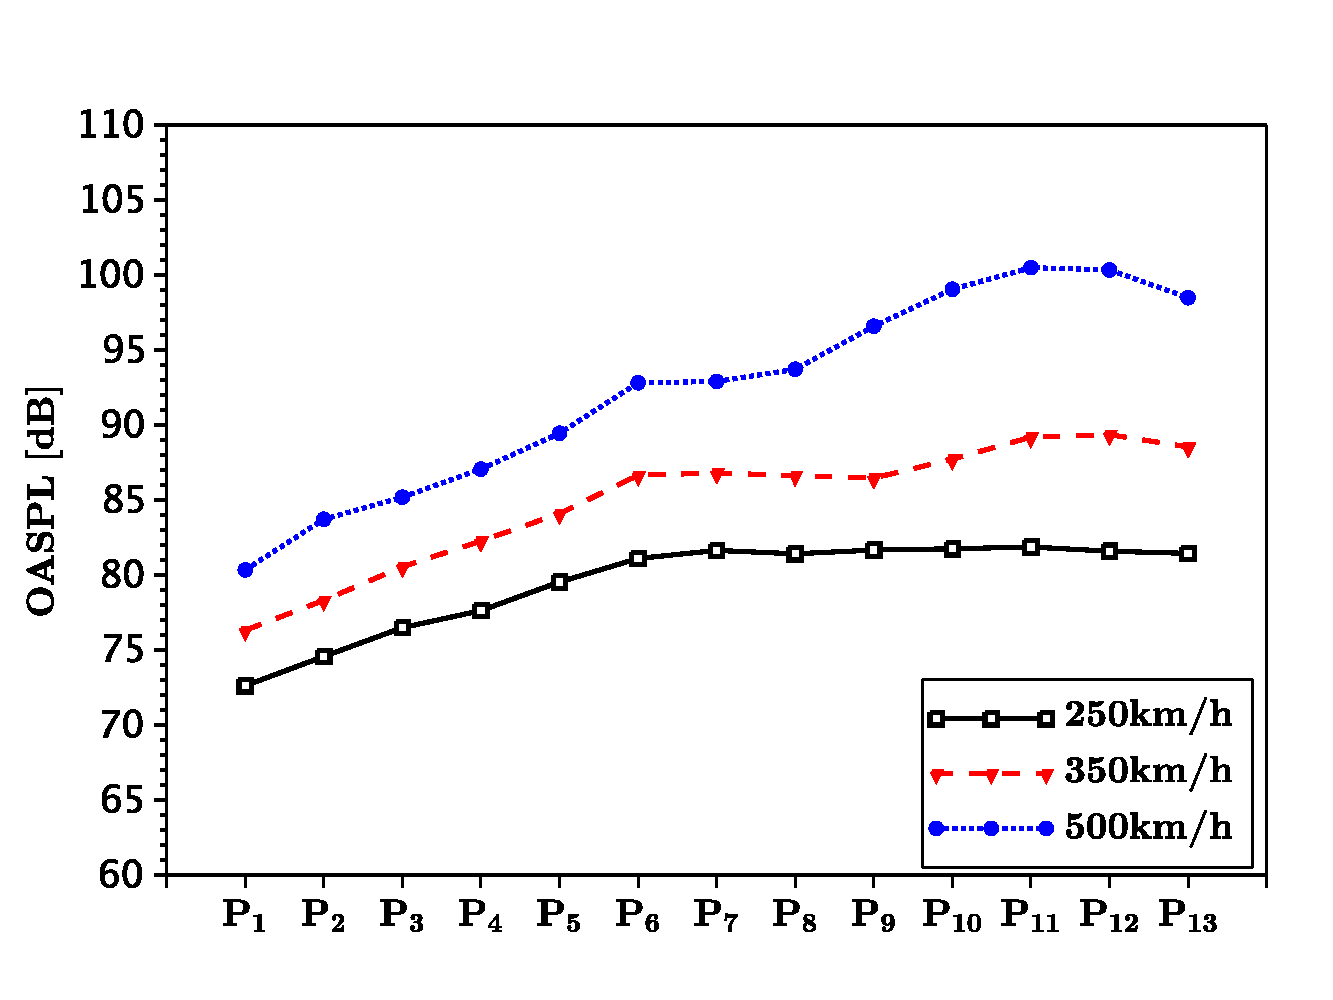
\includegraphics[width=\linewidth]{Figures/oaspl_b.pdf}
    \neusubfigcaption{fig:ch0-four-subfig-b}{工况二}
  \end{neusubfigure}
  \par\vspace{2bp}

  \begin{neusubfigure}{0.49\linewidth}
    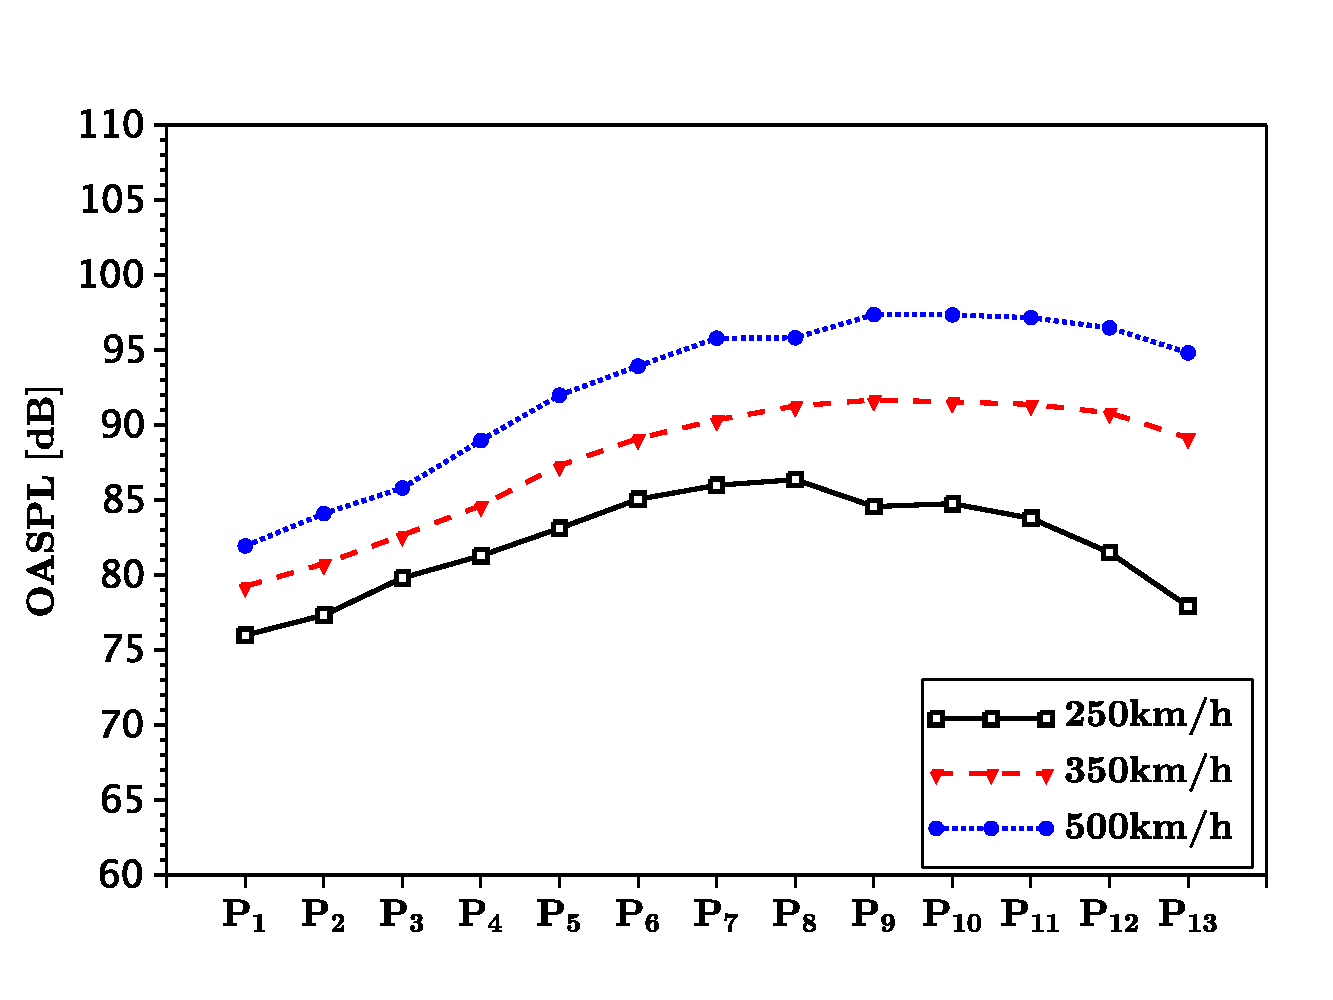
\includegraphics[width=\linewidth]{Figures/oaspl_c.pdf}
    \neusubfigcaption{fig:ch0-four-subfig-c}{工况三}
  \end{neusubfigure}
  \hfill
  \begin{neusubfigure}{0.49\linewidth}
    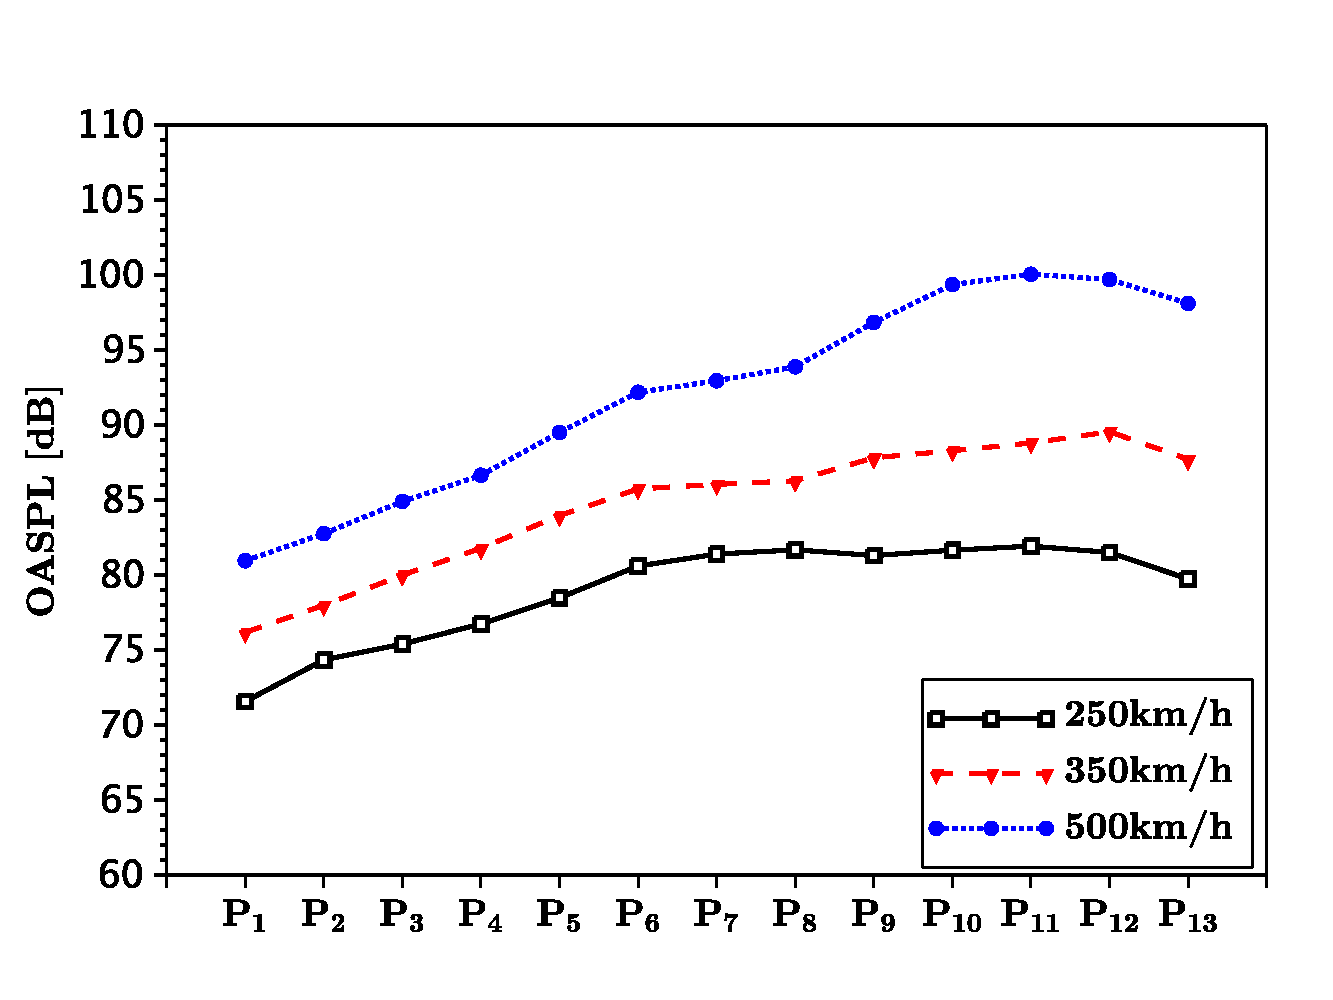
\includegraphics[width=\linewidth]{Figures/oaspl_d.pdf}
    \neusubfigcaption{fig:ch0-four-subfig-d}{工况四}
  \end{neusubfigure}
  \neufigcaption{fig:ch0-four-subfigures}{二乘二子图排版样例}{Example of Two-by-Two Subfigures}
\end{figure}

\neufigref{fig:ch0-four-subfigures} 展示了四幅子图的二乘二排布。
例如 \neusubfigref{fig:ch0-four-subfig-a} 至 \neusubfigref{fig:ch0-four-subfig-d} 可分别引用到四个子图。
排版时建议注意以下几点：
\begin{itemize}
  \item 子图宽度通常可取 \verb|0.48\linewidth| 至 \verb|0.49\linewidth|。
  \item 每行两个子图之间使用 \verb|\hfill| 自动拉开横向间距。
  \item 两行之间可用少量 \verb|\par\vspace| 控制垂直间距。
\end{itemize}

\section{表格排版}

本模板提供 \verb|\neutabcaption{label}{中文题名}{English title}| 用于生成中英文表题。
表题应置于表格上方，正文中使用 \verb|\neutabref{label}| 引用。
表格同样建议使用 \verb|[!htbp]|。如果表格过高导致页底空白，优先考虑缩小字号、调整列宽、拆分表格或使用跨页表格，而不是强制分页。

\subsection{三线表}

\begin{table}[!htbp]
  \centering
  \neutabcaption{tab:ch0-booktabs}{三线表样例}{Example of a Three-Line Table}
  \begin{tabular}{lccc}
    \toprule
    方法       & 准确率（\%）       & 召回率（\%）       & F1 值           \\
    \midrule
    Baseline & 85.2          & 84.1          & 0.846          \\
    Method A & 89.7          & 88.9          & 0.893          \\
    Proposed & \textbf{92.1} & \textbf{91.5} & \textbf{0.918} \\
    \bottomrule
  \end{tabular}
\end{table}

\neutabref{tab:ch0-booktabs} 展示了推荐的三线表格式。
论文中应尽量避免过多竖线，以保持表格简洁。

\subsection{复杂表格}
\begin{table}[!htbp]
  \centering
  \neutabcaption{tab:ch0-complex}{合并单元格与自动换行表格样例}{Example of Merged Cells and Auto-Wrapping Columns}
  \begin{tabularx}{\textwidth}{llXc}
    \toprule
    类别                  & 指标  & 说明                               & 是否必需 \\
    \midrule
    \multirow{2}{*}{图形} & 分辨率 & 位图图片应保证在最终 PDF 中清晰可辨。            & 是    \\
                        & 题名  & 图题使用中英文双语标题，并位于图片下方。             & 是    \\
    \midrule
    \multirow{2}{*}{表格} & 宽度  & 宽表格可使用 \texttt{tabularx} 自动分配列宽。 & 否    \\
                        & 表注  & 表内说明应简明，必要时可在正文中解释。              & 否    \\
    \bottomrule
  \end{tabularx}
\end{table}

\neutabref{tab:ch0-complex} 同时展示了 \verb|\multirow|、\verb|\makecell| 可配合使用的复杂表格场景。
若单元格内容较长，优先使用 \texttt{tabularx} 或 \texttt{p\{...\}} 列类型控制宽度。

\section{公式排版}

公式应使用标准数学环境，并通过 \verb|\label| 设置标签。
引用公式时建议使用模板提供的 \verb|\neueqref{label}|。

\subsection{单行公式}
以分类任务中的交叉熵损失为例，可写为
\begin{equation}
  \mathcal{L}(\theta)
  = - \frac{1}{N}\sum_{i=1}^{N}\sum_{k=1}^{K} y_{ik}\log p_{ik}
  \label{eq:ch0-loss}
\end{equation}

如 \neueqref{eq:ch0-loss} 所示，带编号公式适合放置正文中需要引用的重要定义。

\subsection{多行公式}
循环模型中的状态更新和输出计算可写为
\begin{align}
  h_t       & = \sigma(W_x x_t + W_h h_{t-1} + b), \label{eq:ch0-state} \\
  \hat{y}_t & = \operatorname{softmax}(W_o h_t). \label{eq:ch0-output}
\end{align}

\neueqref{eq:ch0-state} 和 \neueqref{eq:ch0-output} 展示了多行公式的编号方式。
如果多行推导只需要一个编号，可使用 \texttt{aligned} 放在 \texttt{equation} 环境内部。

\subsection{分段函数与矩阵}
分段函数和矩阵经常同时出现在数学定义中，例如
\begin{equation}
  g(x)=
  \begin{cases}
    0, & x < 0,       \\
    x, & 0 \le x < 1, \\
    1, & x \ge 1,
  \end{cases}
  \qquad
  A =
  \begin{bmatrix}
    1 & 0 & 0 \\
    0 & 1 & 0 \\
    0 & 0 & 1
  \end{bmatrix}.
  \label{eq:ch0-piecewise}
\end{equation}

\neueqref{eq:ch0-piecewise} 展示了分段函数和矩阵的常见写法。

\section{算法伪代码}

计算机类论文常需要给出算法步骤。本文档在 \texttt{main.tex} 中加载了 \texttt{algorithm} 和 \texttt{algorithmic} 宏包，可以直接使用如下环境。

\begin{algorithm}[!htbp]
  \caption{样例训练流程}
  \label{alg:ch0-training}
  \begin{algorithmic}[1]
    \REQUIRE Training set $\mathcal{D}$, learning rate $\eta$, maximum epoch $T$
    \ENSURE Model parameters $\theta$
    \STATE Initialize parameters $\theta$
    \FOR{$t = 1$ to $T$}
    \STATE Sample a mini-batch $\mathcal{B}$ from $\mathcal{D}$
    \STATE Compute loss $\mathcal{L}(\theta)$ by \neueqref{eq:ch0-loss}
    \STATE Update $\theta \leftarrow \theta - \eta \nabla_{\theta}\mathcal{L}(\theta)$
    \ENDFOR
    \RETURN $\theta$
  \end{algorithmic}
\end{algorithm}

算法~\ref{alg:ch0-training} 展示了带行号的伪代码。
若需要中文关键字，可在导言区重定义相应命令。

\section{引用、链接与交叉引用}

参考文献引用可使用两种模板命令：
\begin{itemize}
  \item 上标引用使用 \verb|\upcite{key}|，适合放在句末，例如已有研究讨论了神经网络轻量化问题\upcite{guo_2023_research}。
  \item 正文引用使用 \verb|\inlinecite{key}|，适合作为句子成分，例如文献 \inlinecite{thakkar_2018_performance} 给出了系统性能评测案例。
\end{itemize}
多篇文献可写在同一条引用命令中，例如区块链平台相关研究\upcite{zheng_2019_nutbaas,thakkar_2018_performance}。

交叉引用建议统一使用模板命令：
\begin{itemize}
  \item 图引用：\verb|\neufigref{fig:ch0-pdf}|，效果为 \neufigref{fig:ch0-pdf}。
  \item 子图引用：\verb|\neusubfigref{fig:ch0-four-subfig-a}|，效果为 \neusubfigref{fig:ch0-four-subfig-a}。
  \item 表引用：\verb|\neutabref{tab:ch0-complex}|，效果为 \neutabref{tab:ch0-complex}。
  \item 公式引用：\verb|\neueqref{eq:ch0-loss}|，效果为 \neueqref{eq:ch0-loss}。
  \item 算法引用：当前模板未单独封装算法引用命令，可写作“算法~\ref{alg:ch0-training}”。
\end{itemize}
模板提供的公开命令和环境可参考 \texttt{README.md} 中的“模板命令说明”一节。
|，并从第~\ref{chap:introduction}~章开始组织正式内容。

\section{章节层级与正文段落}

论文正文通常从一级标题开始组织内容，一级标题使用 \verb|\chapter|，二级标题使用 \verb|\section|，三级标题使用 \verb|\subsection|。
本模板会自动设置章标题、节标题、页眉、页码和目录格式，作者只需要关注正文内容。
正文段落首行缩进、行距和中英文字体均由模板统一控制，一般不需要在正文中手动设置字号、字体或段间距。

中文正文可以直接书写；英文术语建议在首次出现时给出全称，例如自然语言处理（Natural Language Processing, NLP）。
行内公式可以写作 $E=mc^2$，行内代码或命令可以使用 \verb|\verb|，例如 \verb|%!TEX root = ./main.tex
\chapter{论文格式样例与模板验证}

本章作为模板的集中样例章，用于快速检查正文中常见排版元素的显示效果。
样例覆盖章节层级、正文段落、列表、脚注、图、表、公式、算法、交叉引用和参考文献引用等内容。
编写正式论文时，可以保留本章作为排版对照；定稿前可在 \texttt{main.tex} 中删除或注释 \verb|\input{chapter0-guide}|，并从第~\ref{chap:introduction}~章开始组织正式内容。

\section{章节层级与正文段落}

论文正文通常从一级标题开始组织内容，一级标题使用 \verb|\chapter|，二级标题使用 \verb|\section|，三级标题使用 \verb|\subsection|。
本模板会自动设置章标题、节标题、页眉、页码和目录格式，作者只需要关注正文内容。
正文段落首行缩进、行距和中英文字体均由模板统一控制，一般不需要在正文中手动设置字号、字体或段间距。

中文正文可以直接书写；英文术语建议在首次出现时给出全称，例如自然语言处理（Natural Language Processing, NLP）。
行内公式可以写作 $E=mc^2$，行内代码或命令可以使用 \verb|\verb|，例如 \verb|\input{chapter0-guide}|。
脚注示例如此处所示\footnote{脚注用于补充说明，不宜放置过长的正文内容。}。
若某页因图表浮动或分页规则没有排满，脚注可能跟随正文排版区而显得略高，这是正常的 LaTeX 页面构建结果。

\subsection{字体、字号与强调}

模板预定义了常用中文字体命令。正式论文中通常不需要手动切换字体；只有在展示样式、术语强调或特殊说明时才建议使用。
当前模板已经为默认宋体和 \verb|\song| 字族配置伪粗体，因此 \verb|\textbf| 或 \verb|\bfseries| 可以用于中文局部强调。
需要注意的是，中文加粗应克制使用；标题层级、术语定义或表格重点值可以适当加粗，大段正文不建议整体加粗。
如果需要更明显的标题式强调，可使用黑体或调整标题层级；如果只是普通正文重点，优先使用 \verb|\textbf|。

\begin{table}[!htbp]
  \centering
  \neutabcaption{tab:ch0-fonts}{字体与强调样例}{Examples of Fonts and Emphasis}
  \begin{tabular}{lll}
    \toprule
    命令             & 显示效果                         & 使用建议       \\
    \midrule
    \verb|\song|   & {\song 宋体文字示例}               & 正文默认字体     \\
    \verb|\textbf| & \textbf{加粗文字示例}              & 局部强调、表格重点值 \\
    \verb|\hei|    & {\hei 黑体文字示例}                & 标题或较强强调场景  \\
    \verb|\kai|    & {\kai 楷体文字示例}                & 摘要、题签或引用语  \\
    \verb|\fs|     & {\fs 仿宋文字示例}                 & 特殊文书类内容    \\
    \verb|\textit| & \textit{Italic text example} & 英文斜体或变量说明  \\
    \bottomrule
  \end{tabular}
\end{table}

\subsection{列表环境}

无序列表适合列出并列事项：
\begin{itemize}
  \item 图题位于图下方，表题位于表上方。
  \item 图表应使用中英文双语标题。
  \item 公式、图、表、算法均应使用标签进行交叉引用。
\end{itemize}

有序列表适合描述步骤：
\begin{enumerate}
  \item 在 \texttt{main.tex} 中填写论文元信息。
  \item 在各章文件中撰写正文内容。
  \item 使用 \texttt{latexmk -xelatex main.tex} 完成编译。
\end{enumerate}

\section{图形排版}

本模板提供 \verb|\neufigcaption{label}{中文题名}{English title}| 用于生成中英文图题。
图题应置于图形下方，正文中使用 \verb|\neufigref{label}| 引用。
图形建议使用 \verb|[!htbp]| 浮动参数，让 LaTeX 在当前位置、页顶、页底或浮动页中选择较合适的位置；除非必须固定位置，否则不建议使用 \verb|[H]|。

\subsection{外部图片}
\begin{figure}[!htbp]
  \centering
  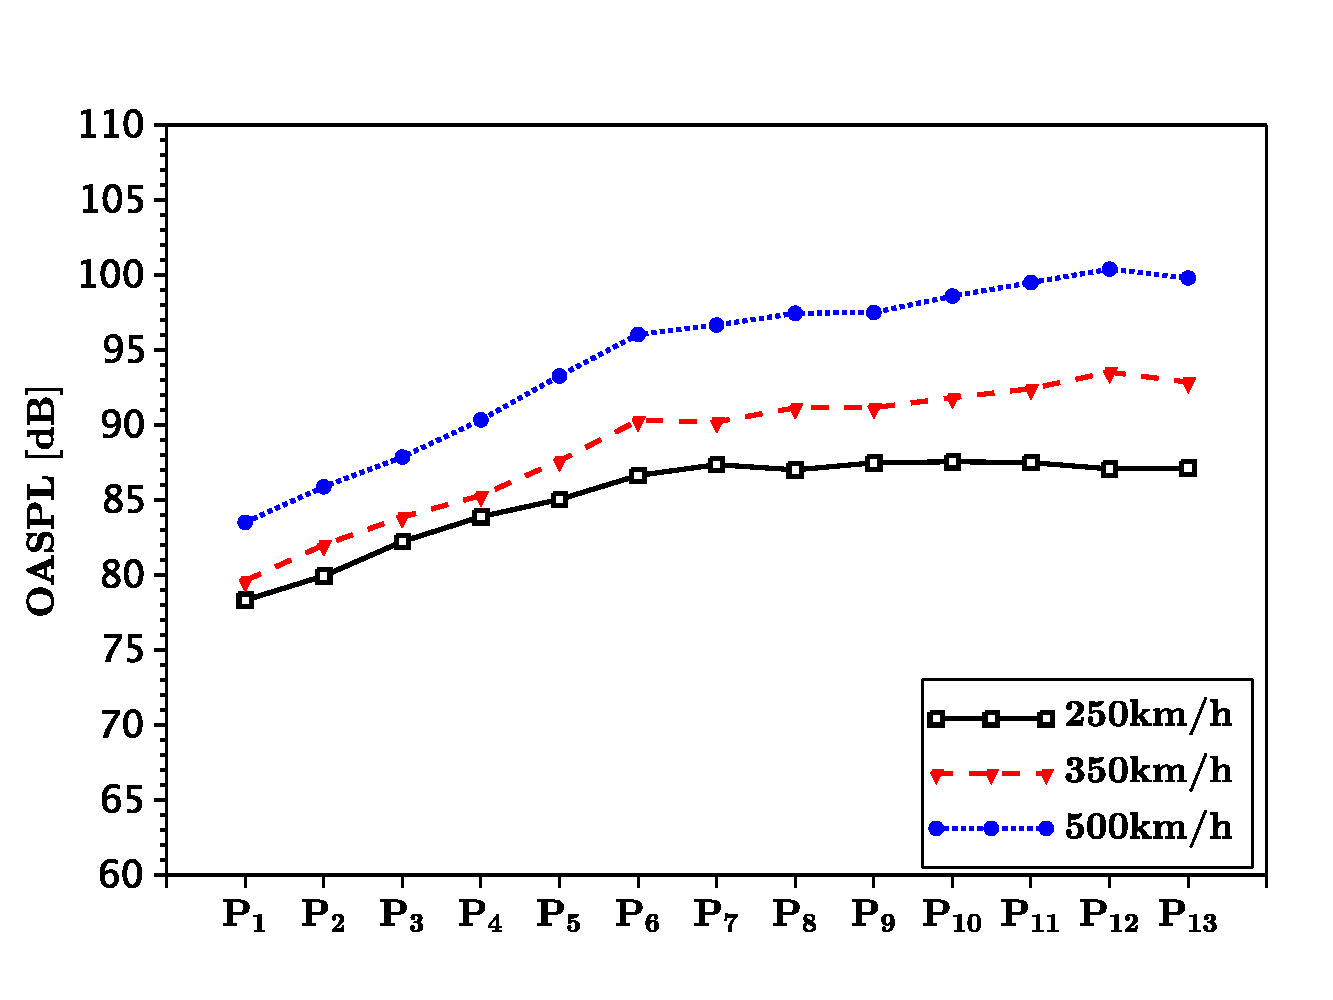
\includegraphics[width=0.55\textwidth]{Figures/oaspl_a.pdf}
  \neufigcaption{fig:ch0-cover}{外部图片插入样例}{Example of Including an External Image}
\end{figure}

\neufigref{fig:ch0-cover} 展示了通过 \verb|\includegraphics| 插入图片文件的方式。
正式论文中建议将图片统一放入 \texttt{Figures} 目录，并使用相对路径引用。

\subsection{PDF 或位图图片}
\begin{figure}[!htbp]
  \centering
  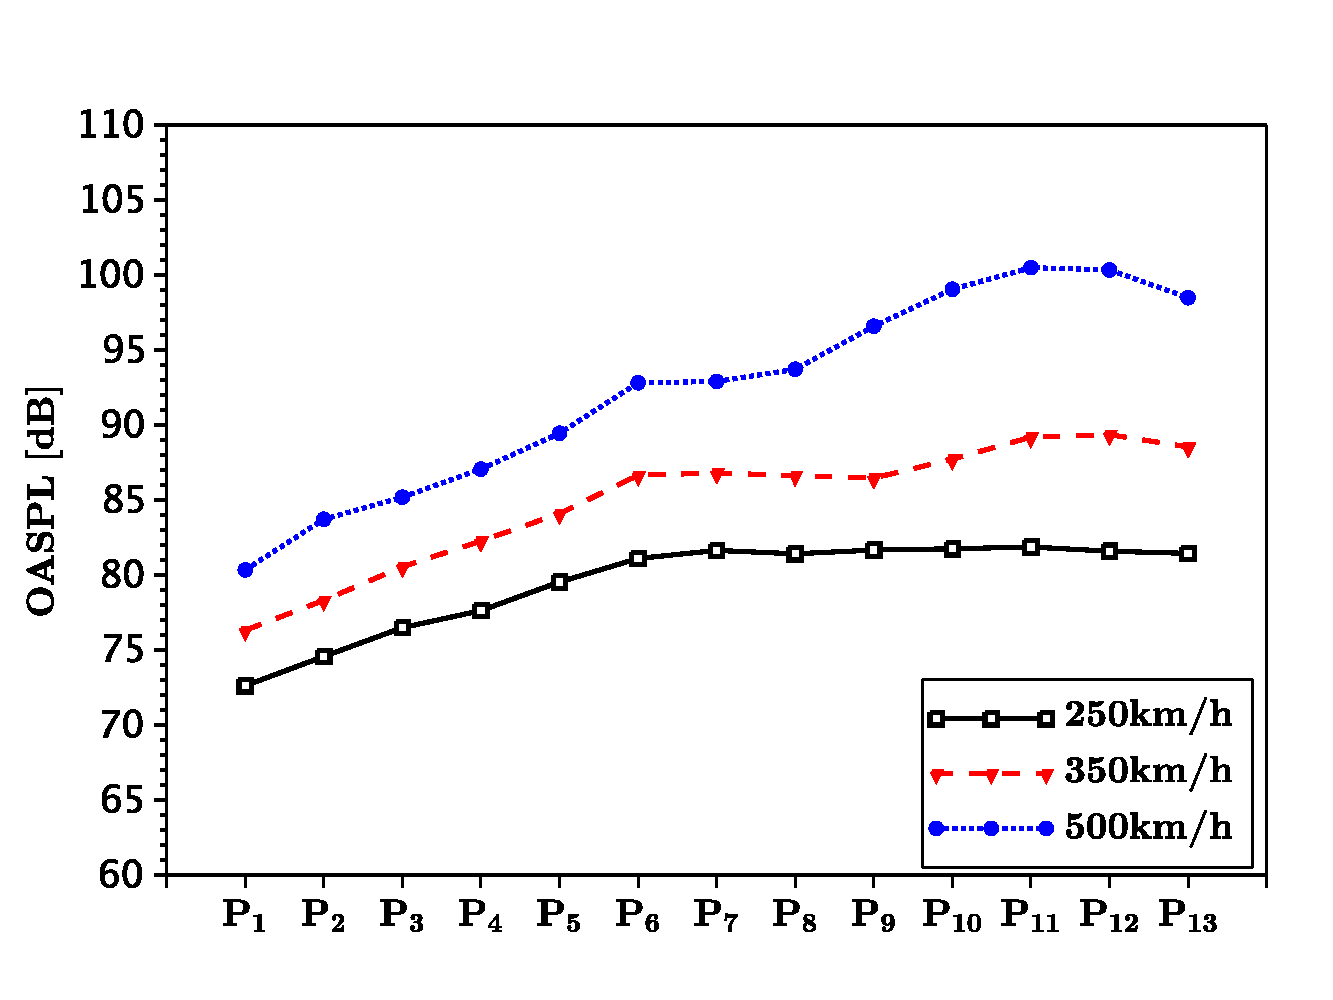
\includegraphics[width=0.55\textwidth]{Figures/oaspl_b.pdf}
  \neufigcaption{fig:ch0-pdf}{PDF 图片插入样例}{Example of Including a PDF Figure}
\end{figure}

PDF、PNG、JPG 等常见图片格式均可通过 \verb|\includegraphics| 插入。
若图片由绘图软件或数据分析程序导出，建议优先使用 PDF 格式以保持较清晰的显示效果。

\subsection{并列图片}
\begin{figure}[!htbp]
  \centering
  \begin{minipage}[t]{0.49\linewidth}
    \centering
    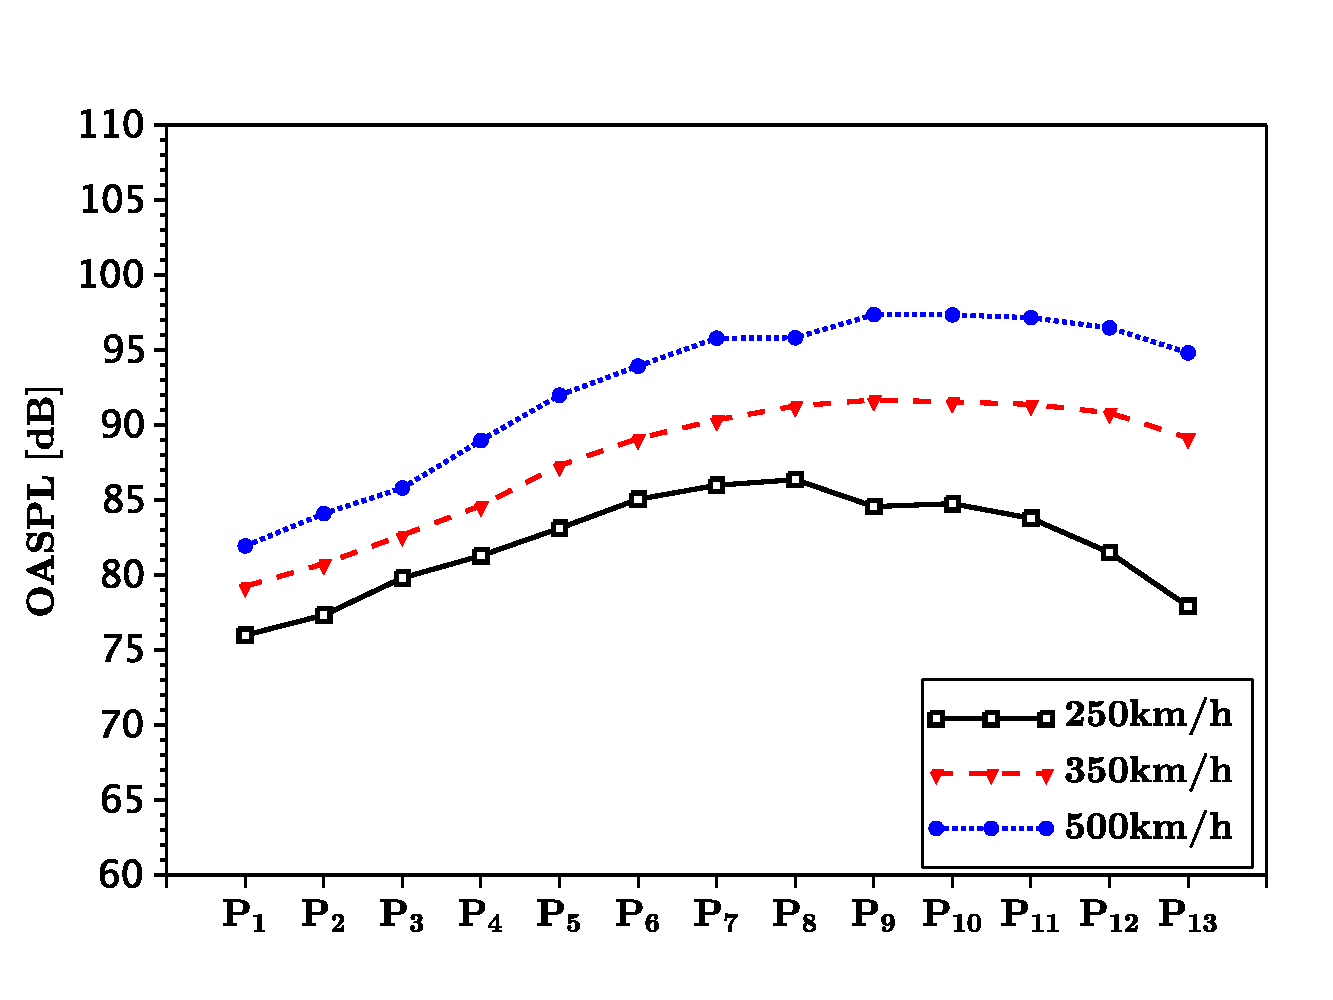
\includegraphics[width=\linewidth]{Figures/oaspl_c.pdf}
  \end{minipage}
  \hfill
  \begin{minipage}[t]{0.49\linewidth}
    \centering
    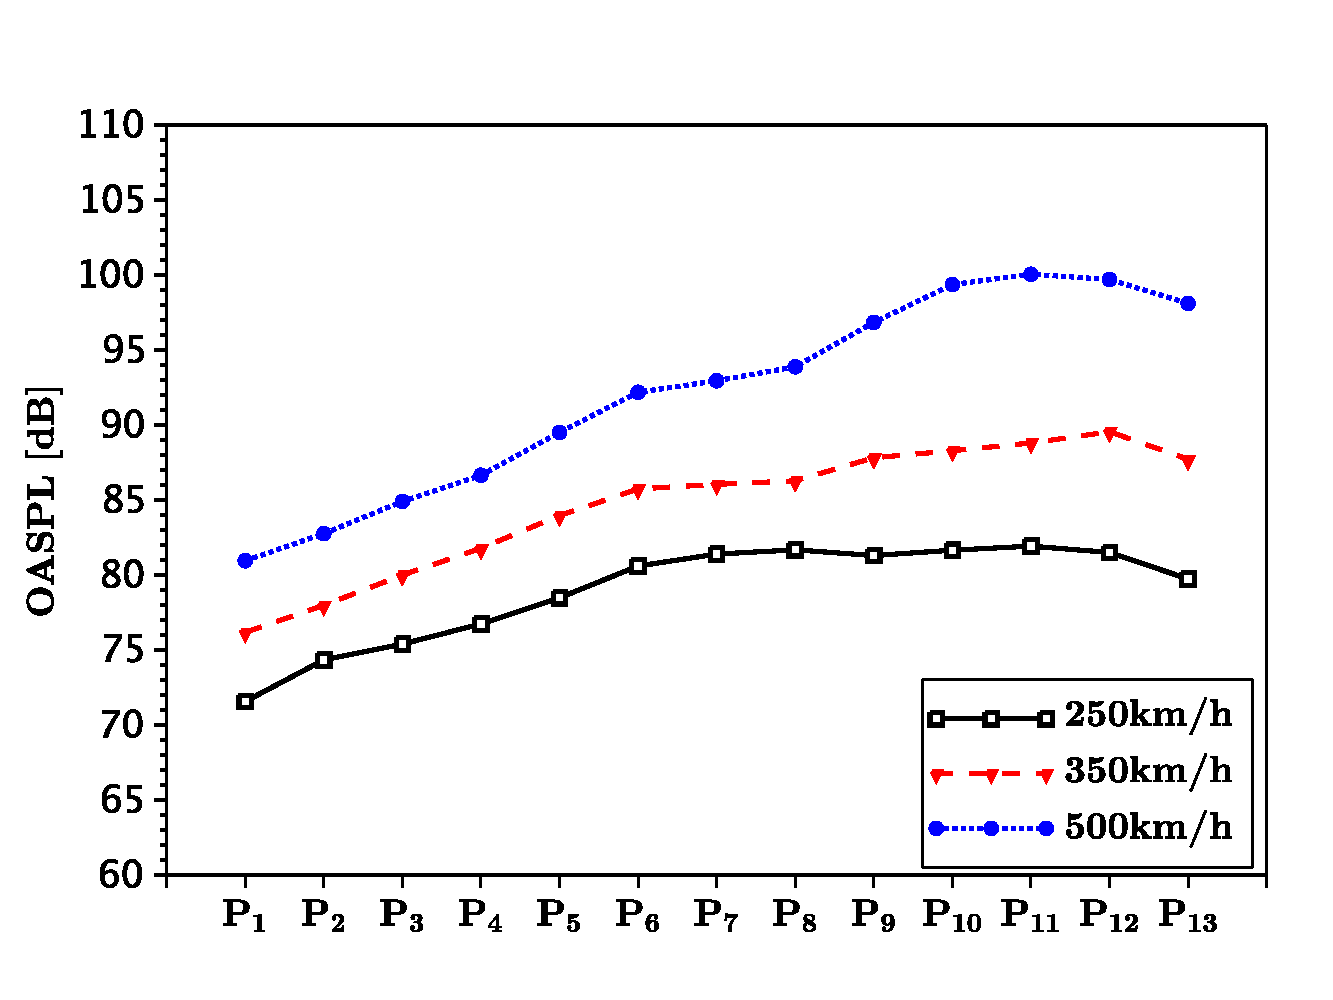
\includegraphics[width=\linewidth]{Figures/oaspl_d.pdf}
  \end{minipage}
  \neufigcaption{fig:ch0-side-by-side}{普通并列图形排版样例}{Example of Side-by-Side Figures}
\end{figure}

\neufigref{fig:ch0-side-by-side} 使用 \texttt{minipage} 完成普通并列排版。
当两幅图共享一个总标题且不需要分别引用时，可使用这种方式。

\subsection{并列子图}
\begin{figure}[!htbp]
  \centering
  \begin{neusubfigure}{0.49\linewidth}
    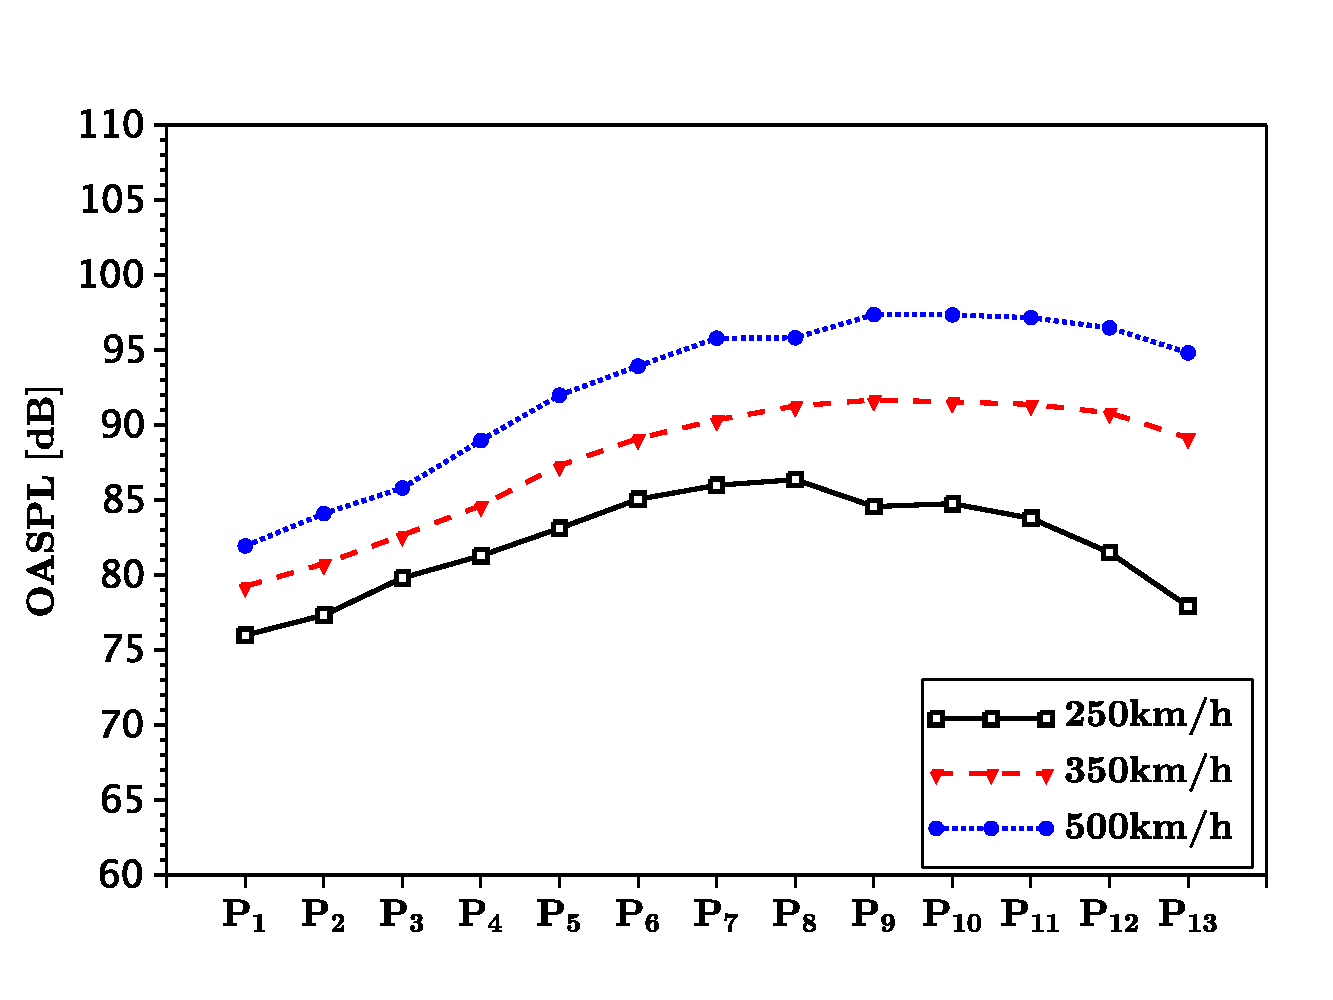
\includegraphics[width=\linewidth]{Figures/oaspl_c.pdf}
    \neusubfigcaption{fig:ch0-side-by-side-a}{工况一}
  \end{neusubfigure}
  \hfill
  \begin{neusubfigure}{0.49\linewidth}
    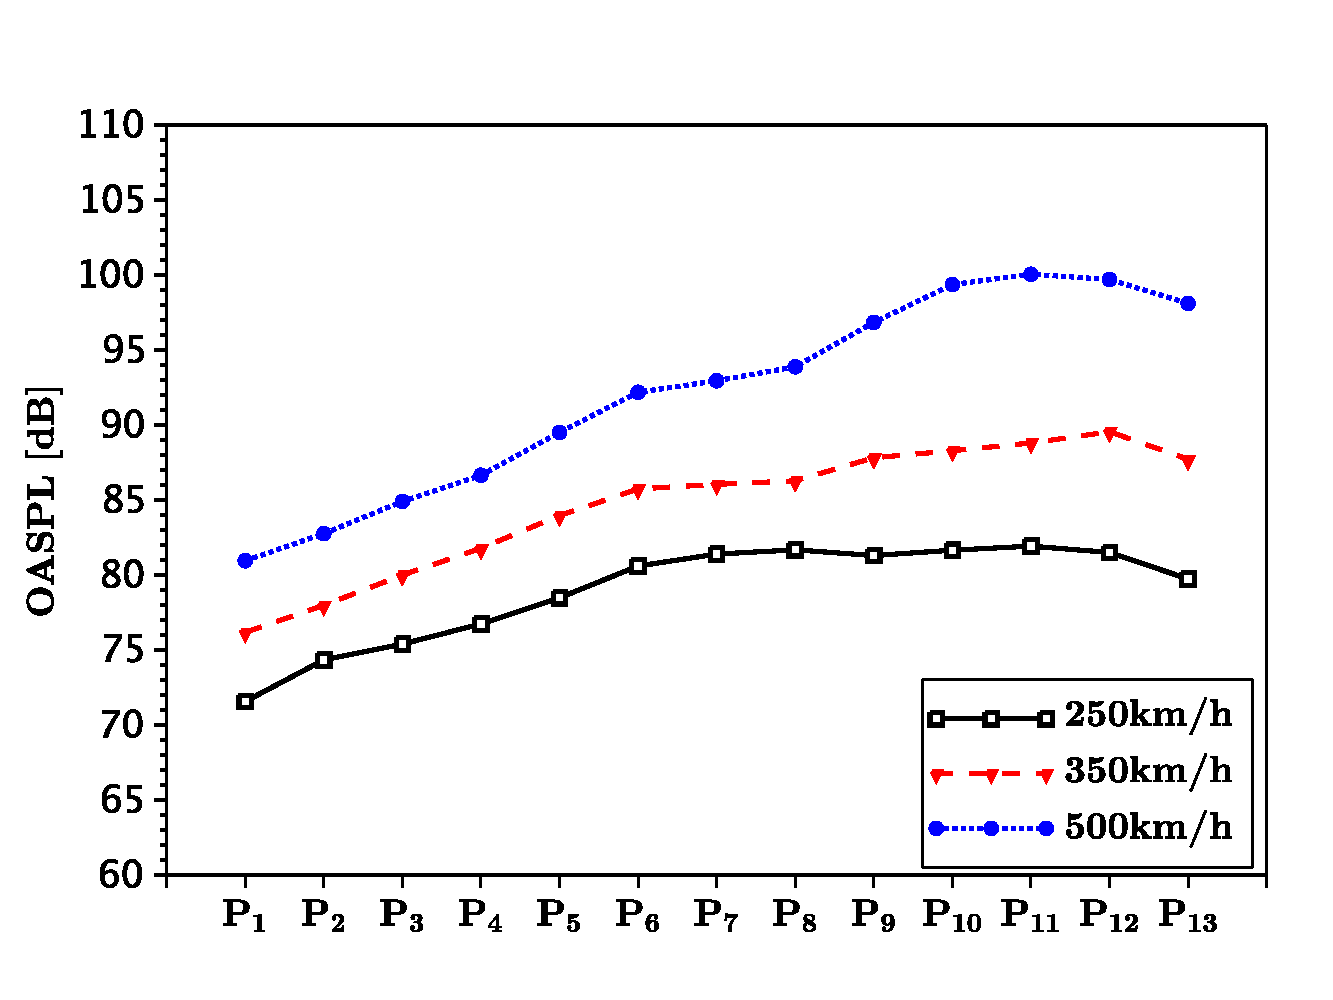
\includegraphics[width=\linewidth]{Figures/oaspl_d.pdf}
    \neusubfigcaption{fig:ch0-side-by-side-b}{工况二}
  \end{neusubfigure}
  \neufigcaption{fig:ch0-subfigures}{并列子图排版样例}{Example of Side-by-Side Subfigures}
\end{figure}

\neufigref{fig:ch0-subfigures} 使用 \texttt{neusubfigure} 完成并列子图排版。
其中 \neusubfigref{fig:ch0-side-by-side-a} 和 \neusubfigref{fig:ch0-side-by-side-b} 可分别引用到子图。
当两幅图共享一个总标题且需要分别引用时，可使用这种方式；如果每幅图需要完全独立的图号，建议拆成两个独立的 \texttt{figure} 环境。

\subsection{二乘二子图}
\begin{figure}[!htbp]
  \centering
  \begin{neusubfigure}{0.49\linewidth}
    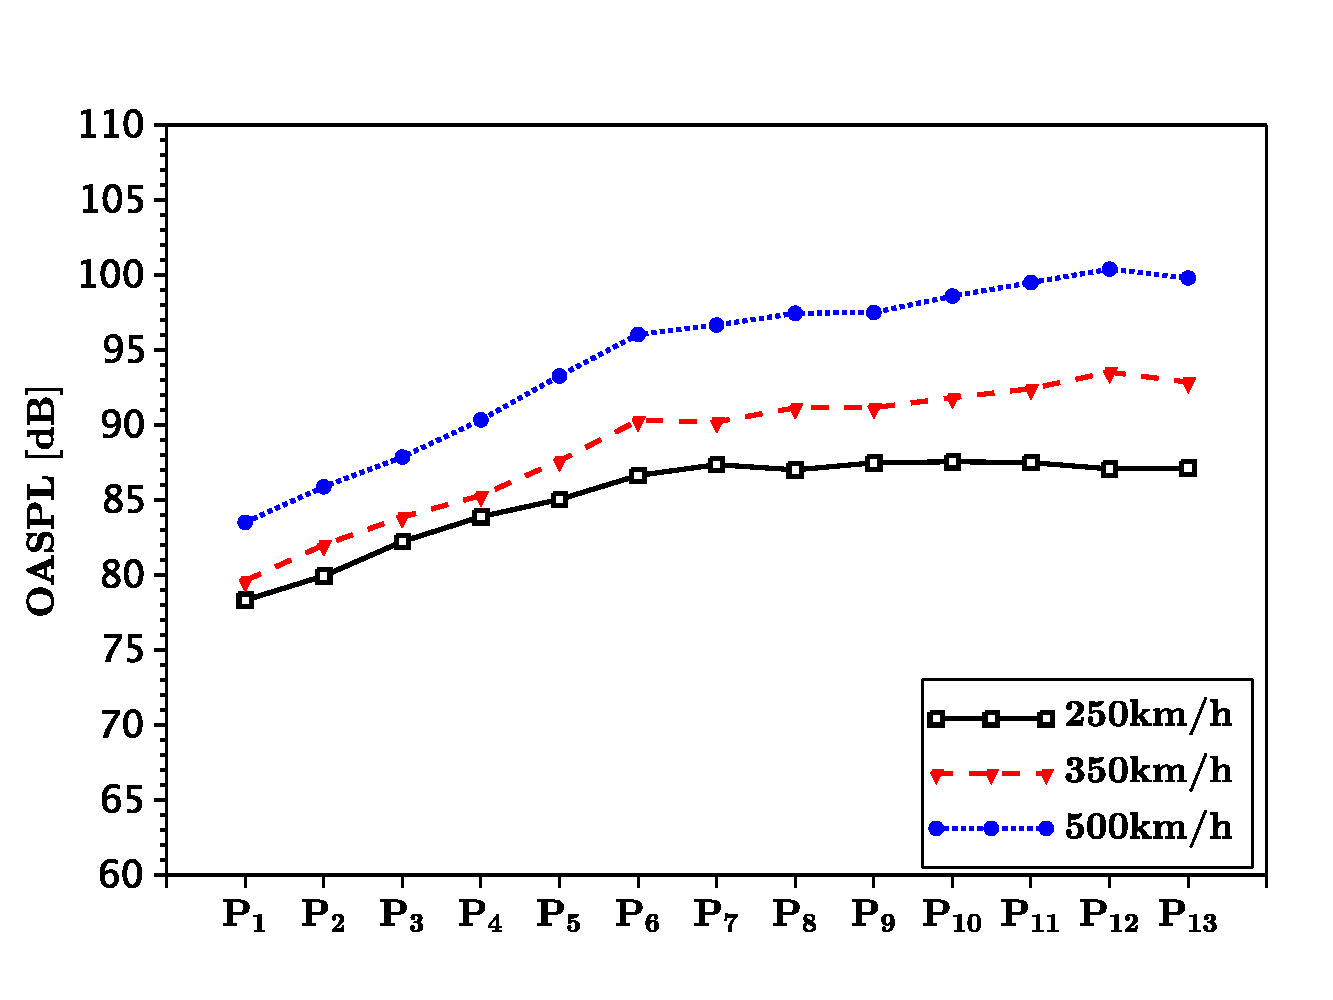
\includegraphics[width=\linewidth]{Figures/oaspl_a.pdf}
    \neusubfigcaption{fig:ch0-four-subfig-a}{工况一}
  \end{neusubfigure}
  \hfill
  \begin{neusubfigure}{0.49\linewidth}
    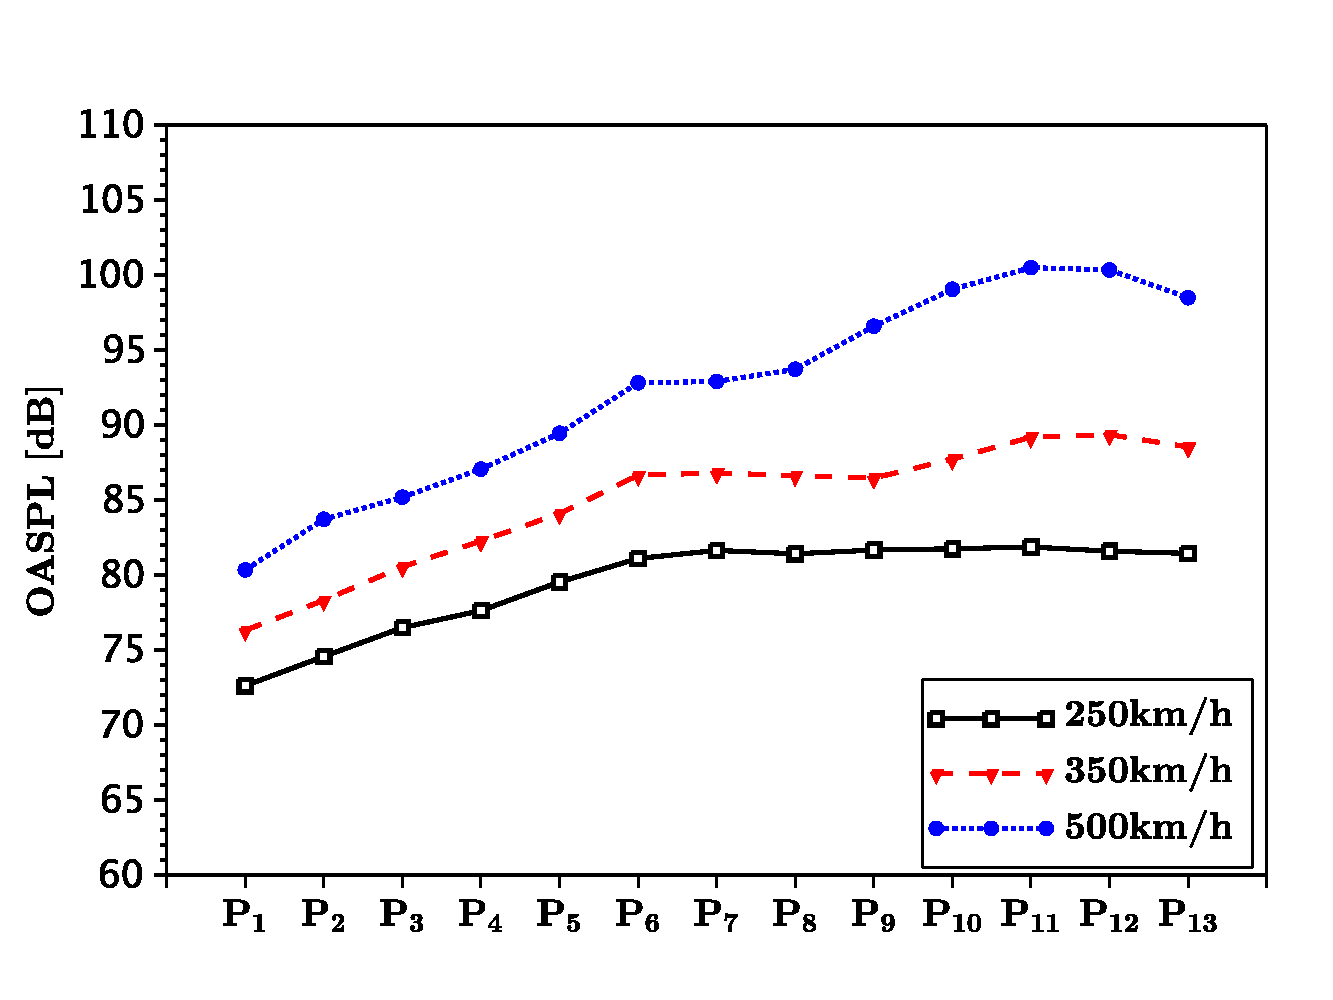
\includegraphics[width=\linewidth]{Figures/oaspl_b.pdf}
    \neusubfigcaption{fig:ch0-four-subfig-b}{工况二}
  \end{neusubfigure}
  \par\vspace{2bp}

  \begin{neusubfigure}{0.49\linewidth}
    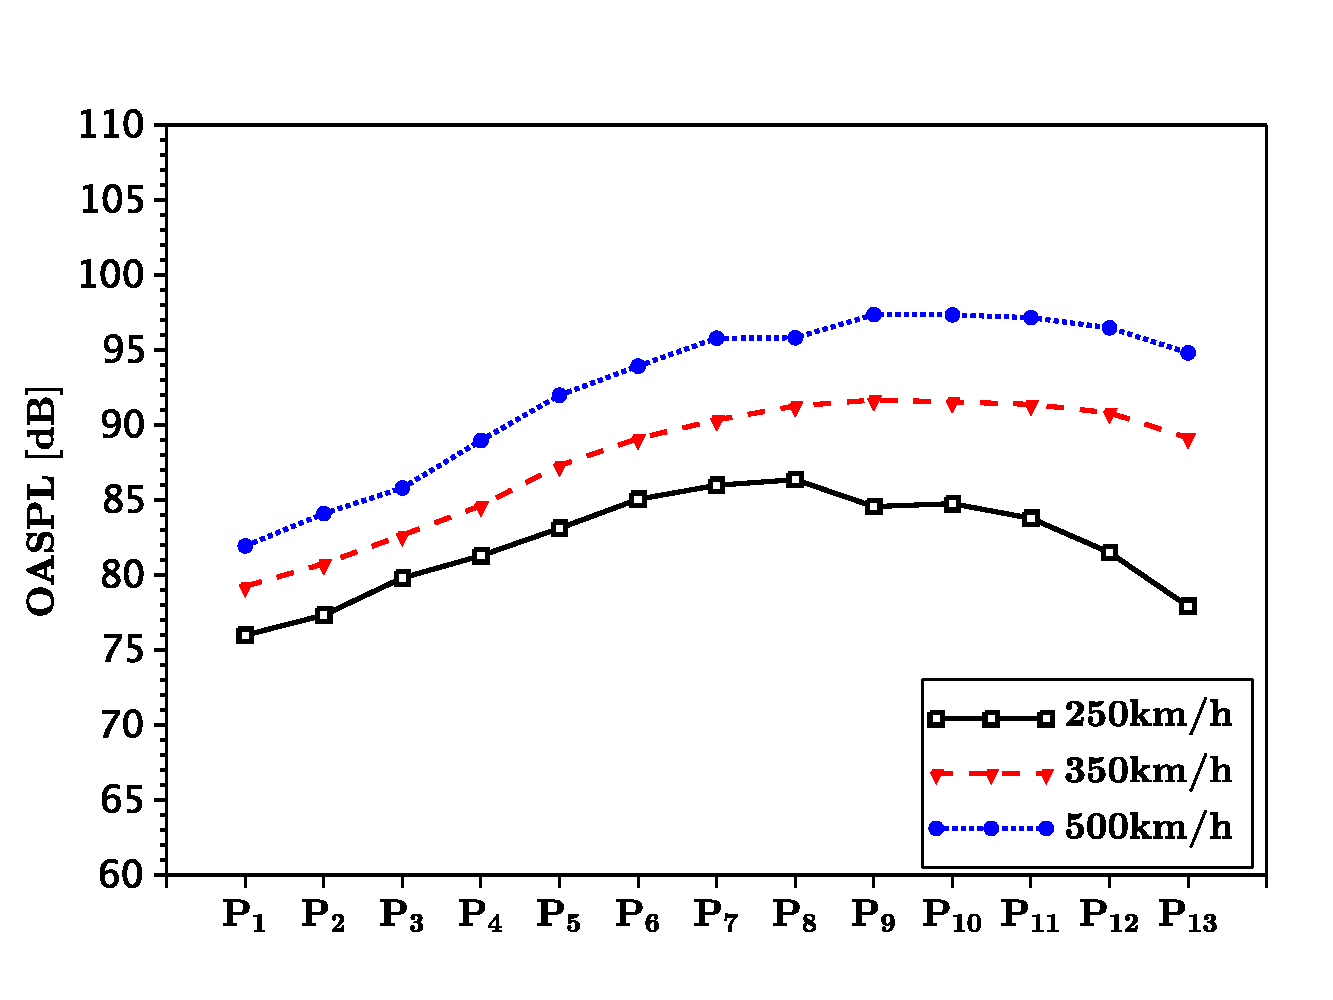
\includegraphics[width=\linewidth]{Figures/oaspl_c.pdf}
    \neusubfigcaption{fig:ch0-four-subfig-c}{工况三}
  \end{neusubfigure}
  \hfill
  \begin{neusubfigure}{0.49\linewidth}
    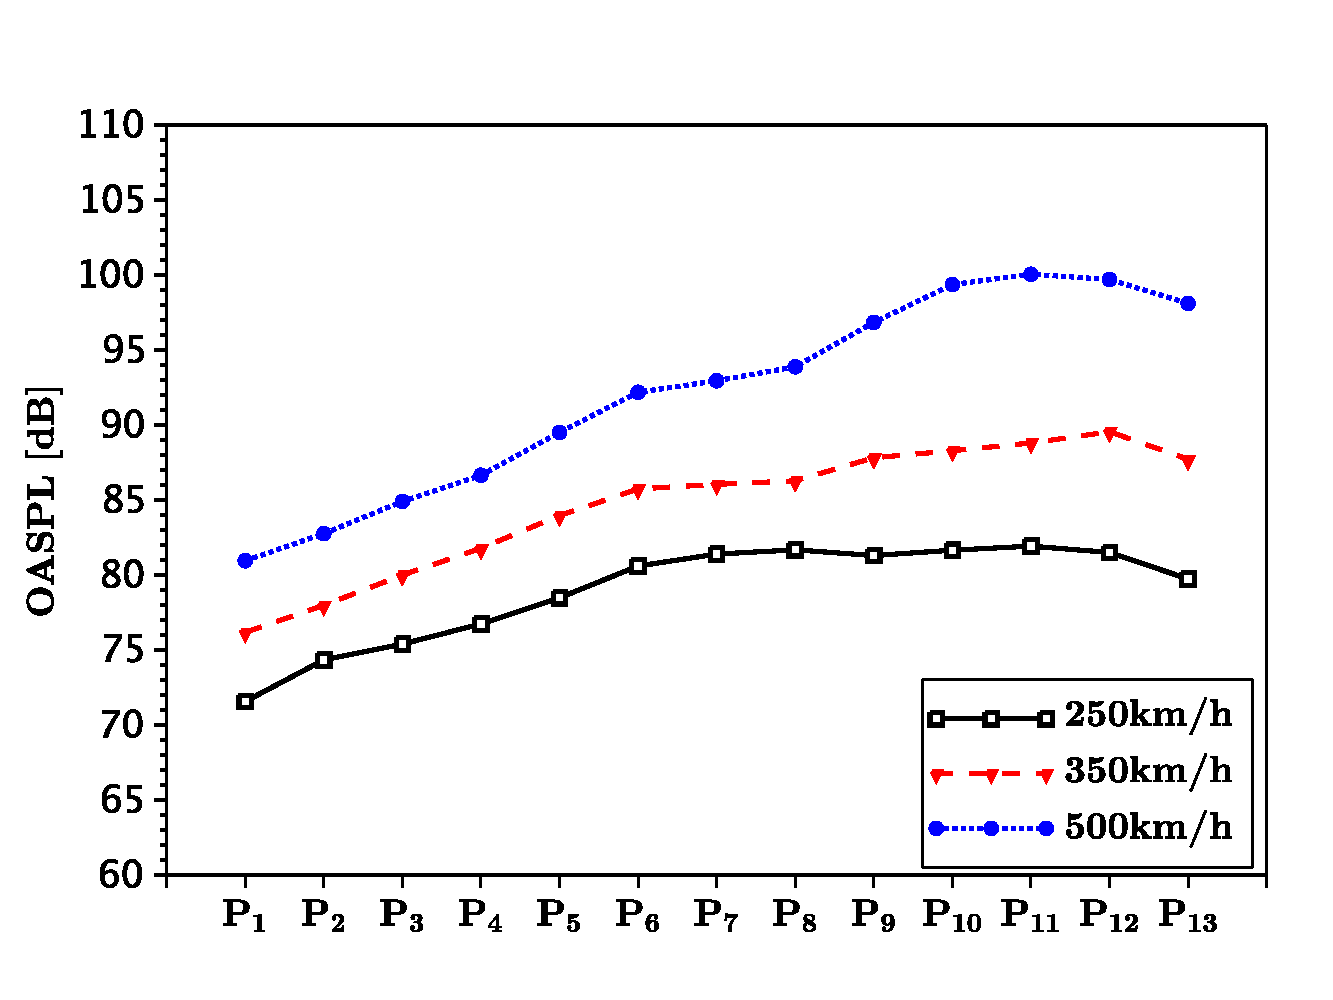
\includegraphics[width=\linewidth]{Figures/oaspl_d.pdf}
    \neusubfigcaption{fig:ch0-four-subfig-d}{工况四}
  \end{neusubfigure}
  \neufigcaption{fig:ch0-four-subfigures}{二乘二子图排版样例}{Example of Two-by-Two Subfigures}
\end{figure}

\neufigref{fig:ch0-four-subfigures} 展示了四幅子图的二乘二排布。
例如 \neusubfigref{fig:ch0-four-subfig-a} 至 \neusubfigref{fig:ch0-four-subfig-d} 可分别引用到四个子图。
排版时建议注意以下几点：
\begin{itemize}
  \item 子图宽度通常可取 \verb|0.48\linewidth| 至 \verb|0.49\linewidth|。
  \item 每行两个子图之间使用 \verb|\hfill| 自动拉开横向间距。
  \item 两行之间可用少量 \verb|\par\vspace| 控制垂直间距。
\end{itemize}

\section{表格排版}

本模板提供 \verb|\neutabcaption{label}{中文题名}{English title}| 用于生成中英文表题。
表题应置于表格上方，正文中使用 \verb|\neutabref{label}| 引用。
表格同样建议使用 \verb|[!htbp]|。如果表格过高导致页底空白，优先考虑缩小字号、调整列宽、拆分表格或使用跨页表格，而不是强制分页。

\subsection{三线表}

\begin{table}[!htbp]
  \centering
  \neutabcaption{tab:ch0-booktabs}{三线表样例}{Example of a Three-Line Table}
  \begin{tabular}{lccc}
    \toprule
    方法       & 准确率（\%）       & 召回率（\%）       & F1 值           \\
    \midrule
    Baseline & 85.2          & 84.1          & 0.846          \\
    Method A & 89.7          & 88.9          & 0.893          \\
    Proposed & \textbf{92.1} & \textbf{91.5} & \textbf{0.918} \\
    \bottomrule
  \end{tabular}
\end{table}

\neutabref{tab:ch0-booktabs} 展示了推荐的三线表格式。
论文中应尽量避免过多竖线，以保持表格简洁。

\subsection{复杂表格}
\begin{table}[!htbp]
  \centering
  \neutabcaption{tab:ch0-complex}{合并单元格与自动换行表格样例}{Example of Merged Cells and Auto-Wrapping Columns}
  \begin{tabularx}{\textwidth}{llXc}
    \toprule
    类别                  & 指标  & 说明                               & 是否必需 \\
    \midrule
    \multirow{2}{*}{图形} & 分辨率 & 位图图片应保证在最终 PDF 中清晰可辨。            & 是    \\
                        & 题名  & 图题使用中英文双语标题，并位于图片下方。             & 是    \\
    \midrule
    \multirow{2}{*}{表格} & 宽度  & 宽表格可使用 \texttt{tabularx} 自动分配列宽。 & 否    \\
                        & 表注  & 表内说明应简明，必要时可在正文中解释。              & 否    \\
    \bottomrule
  \end{tabularx}
\end{table}

\neutabref{tab:ch0-complex} 同时展示了 \verb|\multirow|、\verb|\makecell| 可配合使用的复杂表格场景。
若单元格内容较长，优先使用 \texttt{tabularx} 或 \texttt{p\{...\}} 列类型控制宽度。

\section{公式排版}

公式应使用标准数学环境，并通过 \verb|\label| 设置标签。
引用公式时建议使用模板提供的 \verb|\neueqref{label}|。

\subsection{单行公式}
以分类任务中的交叉熵损失为例，可写为
\begin{equation}
  \mathcal{L}(\theta)
  = - \frac{1}{N}\sum_{i=1}^{N}\sum_{k=1}^{K} y_{ik}\log p_{ik}
  \label{eq:ch0-loss}
\end{equation}

如 \neueqref{eq:ch0-loss} 所示，带编号公式适合放置正文中需要引用的重要定义。

\subsection{多行公式}
循环模型中的状态更新和输出计算可写为
\begin{align}
  h_t       & = \sigma(W_x x_t + W_h h_{t-1} + b), \label{eq:ch0-state} \\
  \hat{y}_t & = \operatorname{softmax}(W_o h_t). \label{eq:ch0-output}
\end{align}

\neueqref{eq:ch0-state} 和 \neueqref{eq:ch0-output} 展示了多行公式的编号方式。
如果多行推导只需要一个编号，可使用 \texttt{aligned} 放在 \texttt{equation} 环境内部。

\subsection{分段函数与矩阵}
分段函数和矩阵经常同时出现在数学定义中，例如
\begin{equation}
  g(x)=
  \begin{cases}
    0, & x < 0,       \\
    x, & 0 \le x < 1, \\
    1, & x \ge 1,
  \end{cases}
  \qquad
  A =
  \begin{bmatrix}
    1 & 0 & 0 \\
    0 & 1 & 0 \\
    0 & 0 & 1
  \end{bmatrix}.
  \label{eq:ch0-piecewise}
\end{equation}

\neueqref{eq:ch0-piecewise} 展示了分段函数和矩阵的常见写法。

\section{算法伪代码}

计算机类论文常需要给出算法步骤。本文档在 \texttt{main.tex} 中加载了 \texttt{algorithm} 和 \texttt{algorithmic} 宏包，可以直接使用如下环境。

\begin{algorithm}[!htbp]
  \caption{样例训练流程}
  \label{alg:ch0-training}
  \begin{algorithmic}[1]
    \REQUIRE Training set $\mathcal{D}$, learning rate $\eta$, maximum epoch $T$
    \ENSURE Model parameters $\theta$
    \STATE Initialize parameters $\theta$
    \FOR{$t = 1$ to $T$}
    \STATE Sample a mini-batch $\mathcal{B}$ from $\mathcal{D}$
    \STATE Compute loss $\mathcal{L}(\theta)$ by \neueqref{eq:ch0-loss}
    \STATE Update $\theta \leftarrow \theta - \eta \nabla_{\theta}\mathcal{L}(\theta)$
    \ENDFOR
    \RETURN $\theta$
  \end{algorithmic}
\end{algorithm}

算法~\ref{alg:ch0-training} 展示了带行号的伪代码。
若需要中文关键字，可在导言区重定义相应命令。

\section{引用、链接与交叉引用}

参考文献引用可使用两种模板命令：
\begin{itemize}
  \item 上标引用使用 \verb|\upcite{key}|，适合放在句末，例如已有研究讨论了神经网络轻量化问题\upcite{guo_2023_research}。
  \item 正文引用使用 \verb|\inlinecite{key}|，适合作为句子成分，例如文献 \inlinecite{thakkar_2018_performance} 给出了系统性能评测案例。
\end{itemize}
多篇文献可写在同一条引用命令中，例如区块链平台相关研究\upcite{zheng_2019_nutbaas,thakkar_2018_performance}。

交叉引用建议统一使用模板命令：
\begin{itemize}
  \item 图引用：\verb|\neufigref{fig:ch0-pdf}|，效果为 \neufigref{fig:ch0-pdf}。
  \item 子图引用：\verb|\neusubfigref{fig:ch0-four-subfig-a}|，效果为 \neusubfigref{fig:ch0-four-subfig-a}。
  \item 表引用：\verb|\neutabref{tab:ch0-complex}|，效果为 \neutabref{tab:ch0-complex}。
  \item 公式引用：\verb|\neueqref{eq:ch0-loss}|，效果为 \neueqref{eq:ch0-loss}。
  \item 算法引用：当前模板未单独封装算法引用命令，可写作“算法~\ref{alg:ch0-training}”。
\end{itemize}
模板提供的公开命令和环境可参考 \texttt{README.md} 中的“模板命令说明”一节。
|。
脚注示例如此处所示\footnote{脚注用于补充说明，不宜放置过长的正文内容。}。
若某页因图表浮动或分页规则没有排满，脚注可能跟随正文排版区而显得略高，这是正常的 LaTeX 页面构建结果。

\subsection{字体、字号与强调}

模板预定义了常用中文字体命令。正式论文中通常不需要手动切换字体；只有在展示样式、术语强调或特殊说明时才建议使用。
当前模板已经为默认宋体和 \verb|\song| 字族配置伪粗体，因此 \verb|\textbf| 或 \verb|\bfseries| 可以用于中文局部强调。
需要注意的是，中文加粗应克制使用；标题层级、术语定义或表格重点值可以适当加粗，大段正文不建议整体加粗。
如果需要更明显的标题式强调，可使用黑体或调整标题层级；如果只是普通正文重点，优先使用 \verb|\textbf|。

\begin{table}[!htbp]
  \centering
  \neutabcaption{tab:ch0-fonts}{字体与强调样例}{Examples of Fonts and Emphasis}
  \begin{tabular}{lll}
    \toprule
    命令             & 显示效果                         & 使用建议       \\
    \midrule
    \verb|\song|   & {\song 宋体文字示例}               & 正文默认字体     \\
    \verb|\textbf| & \textbf{加粗文字示例}              & 局部强调、表格重点值 \\
    \verb|\hei|    & {\hei 黑体文字示例}                & 标题或较强强调场景  \\
    \verb|\kai|    & {\kai 楷体文字示例}                & 摘要、题签或引用语  \\
    \verb|\fs|     & {\fs 仿宋文字示例}                 & 特殊文书类内容    \\
    \verb|\textit| & \textit{Italic text example} & 英文斜体或变量说明  \\
    \bottomrule
  \end{tabular}
\end{table}

\subsection{列表环境}

无序列表适合列出并列事项：
\begin{itemize}
  \item 图题位于图下方，表题位于表上方。
  \item 图表应使用中英文双语标题。
  \item 公式、图、表、算法均应使用标签进行交叉引用。
\end{itemize}

有序列表适合描述步骤：
\begin{enumerate}
  \item 在 \texttt{main.tex} 中填写论文元信息。
  \item 在各章文件中撰写正文内容。
  \item 使用 \texttt{latexmk -xelatex main.tex} 完成编译。
\end{enumerate}

\section{图形排版}

本模板提供 \verb|\neufigcaption{label}{中文题名}{English title}| 用于生成中英文图题。
图题应置于图形下方，正文中使用 \verb|\neufigref{label}| 引用。
图形建议使用 \verb|[!htbp]| 浮动参数，让 LaTeX 在当前位置、页顶、页底或浮动页中选择较合适的位置；除非必须固定位置，否则不建议使用 \verb|[H]|。

\subsection{外部图片}
\begin{figure}[!htbp]
  \centering
  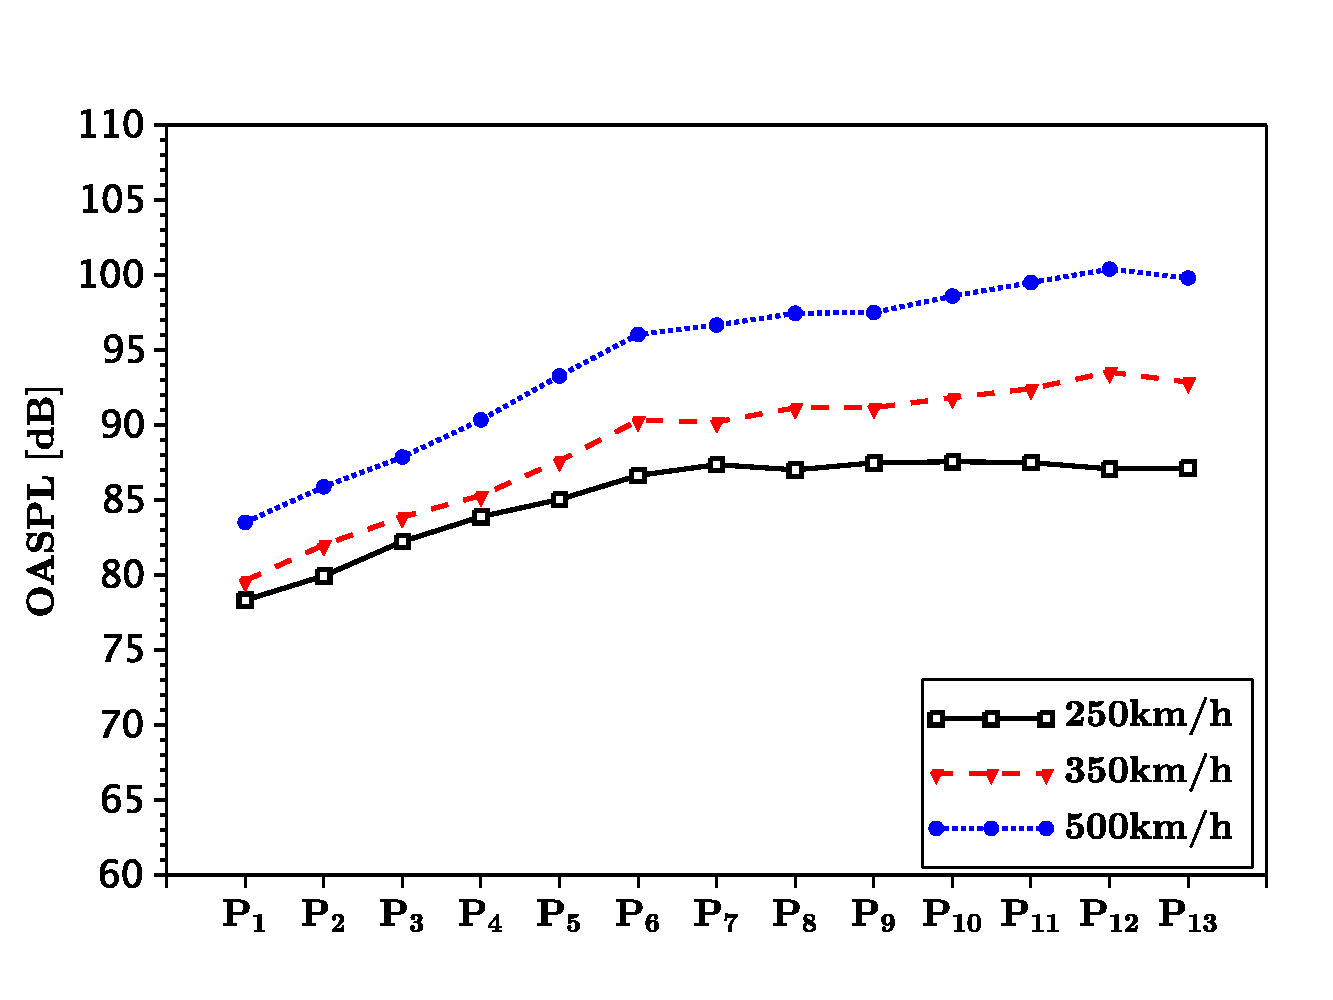
\includegraphics[width=0.55\textwidth]{Figures/oaspl_a.pdf}
  \neufigcaption{fig:ch0-cover}{外部图片插入样例}{Example of Including an External Image}
\end{figure}

\neufigref{fig:ch0-cover} 展示了通过 \verb|\includegraphics| 插入图片文件的方式。
正式论文中建议将图片统一放入 \texttt{Figures} 目录，并使用相对路径引用。

\subsection{PDF 或位图图片}
\begin{figure}[!htbp]
  \centering
  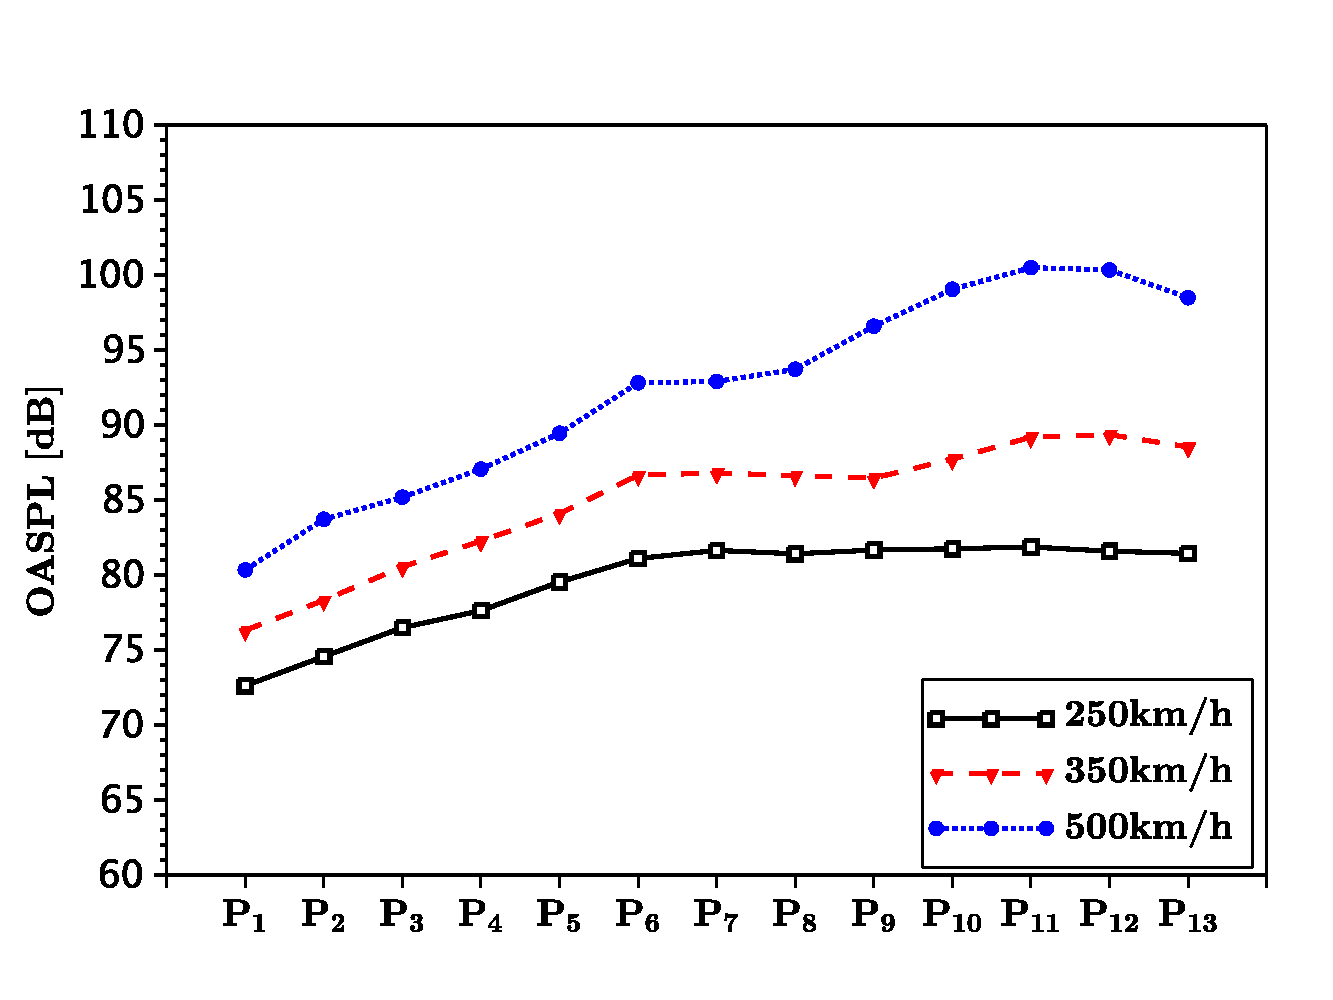
\includegraphics[width=0.55\textwidth]{Figures/oaspl_b.pdf}
  \neufigcaption{fig:ch0-pdf}{PDF 图片插入样例}{Example of Including a PDF Figure}
\end{figure}

PDF、PNG、JPG 等常见图片格式均可通过 \verb|\includegraphics| 插入。
若图片由绘图软件或数据分析程序导出，建议优先使用 PDF 格式以保持较清晰的显示效果。

\subsection{并列图片}
\begin{figure}[!htbp]
  \centering
  \begin{minipage}[t]{0.49\linewidth}
    \centering
    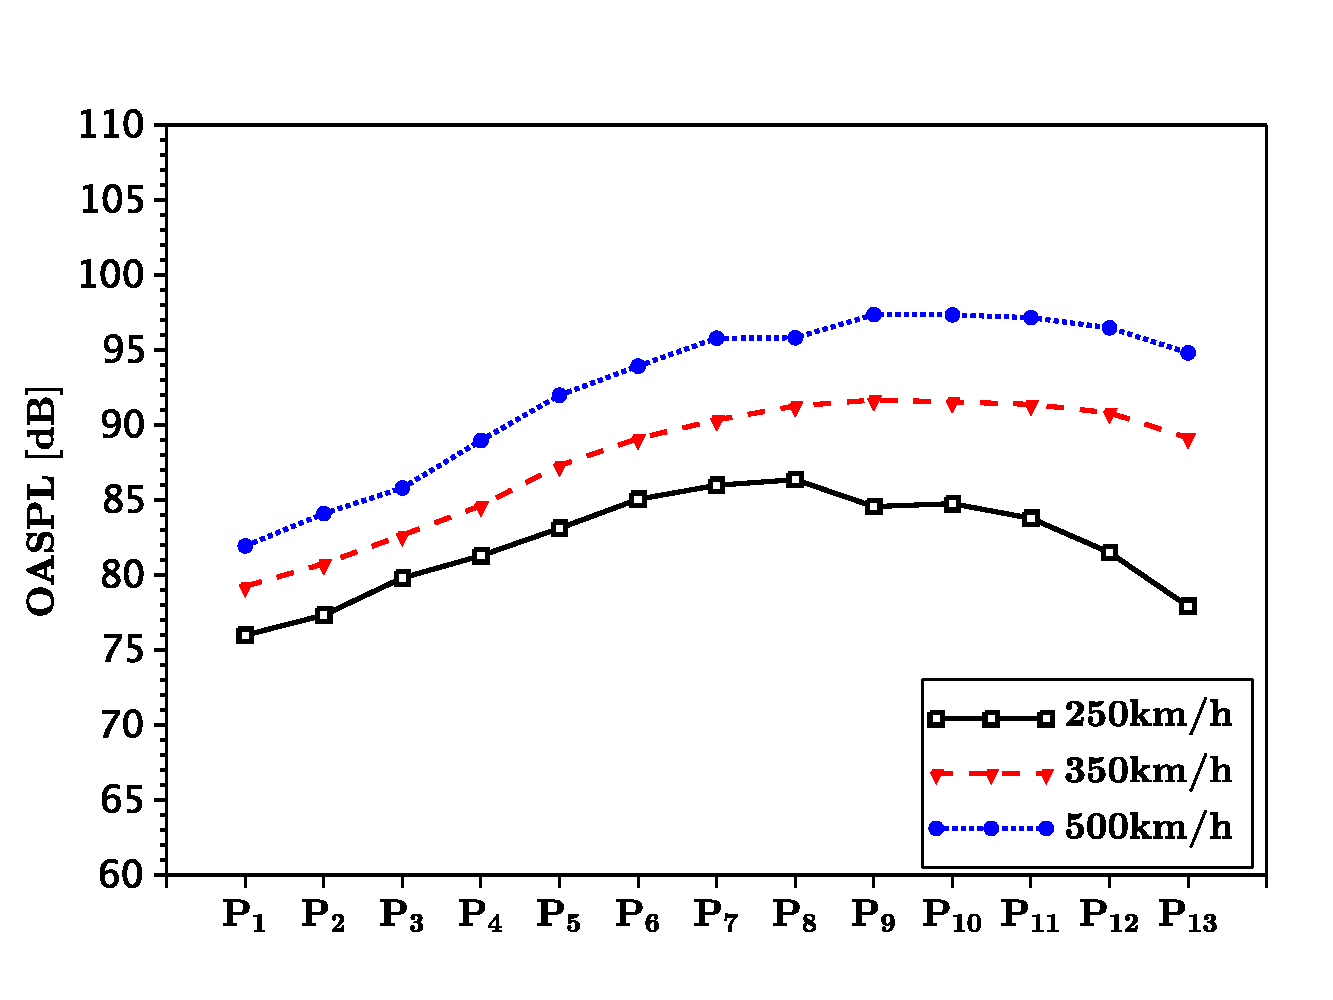
\includegraphics[width=\linewidth]{Figures/oaspl_c.pdf}
  \end{minipage}
  \hfill
  \begin{minipage}[t]{0.49\linewidth}
    \centering
    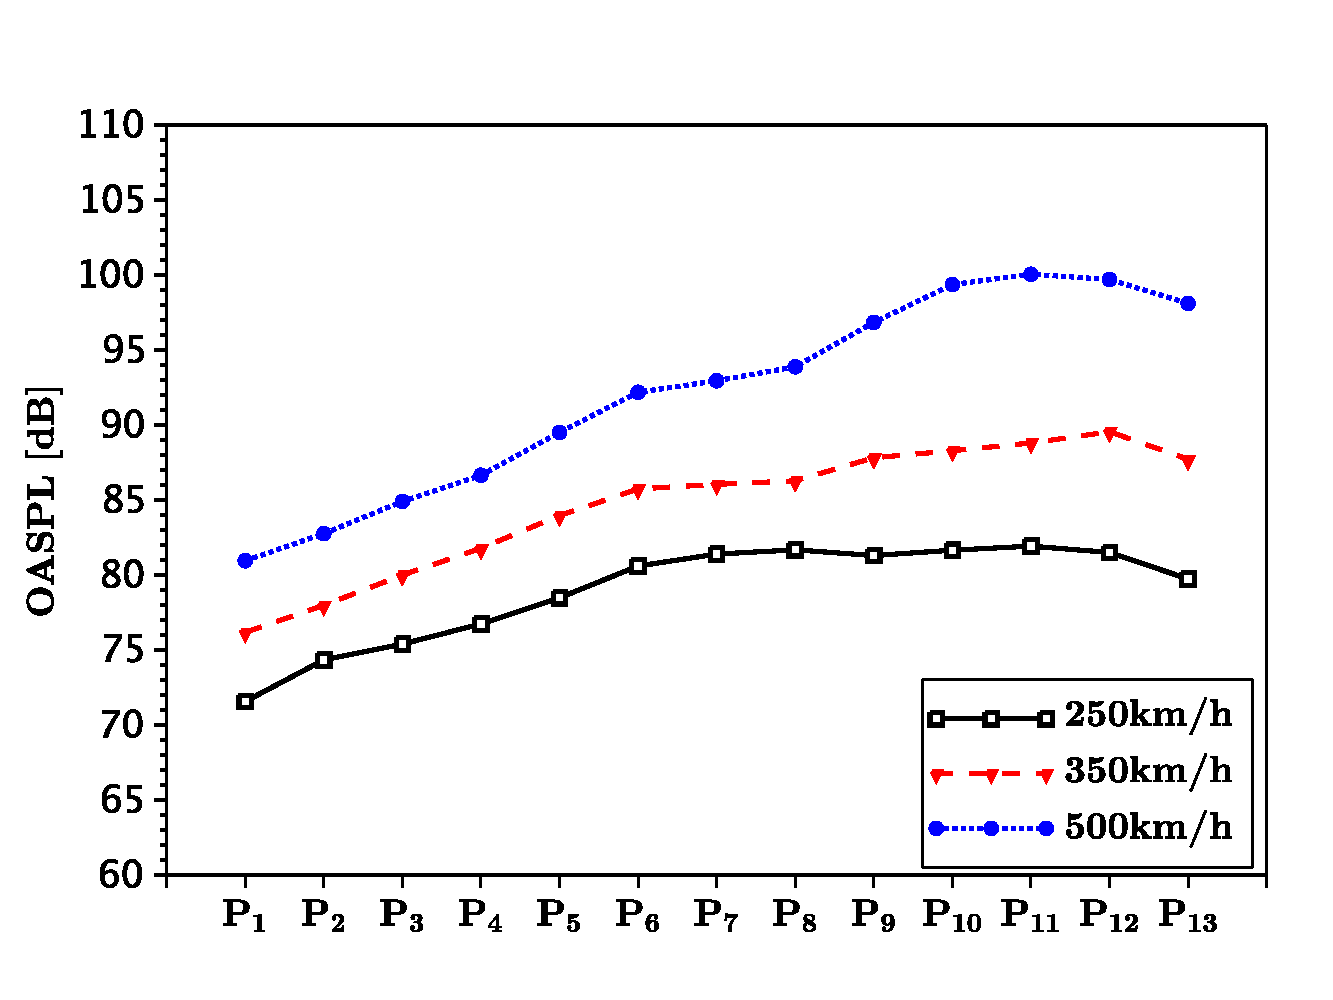
\includegraphics[width=\linewidth]{Figures/oaspl_d.pdf}
  \end{minipage}
  \neufigcaption{fig:ch0-side-by-side}{普通并列图形排版样例}{Example of Side-by-Side Figures}
\end{figure}

\neufigref{fig:ch0-side-by-side} 使用 \texttt{minipage} 完成普通并列排版。
当两幅图共享一个总标题且不需要分别引用时，可使用这种方式。

\subsection{并列子图}
\begin{figure}[!htbp]
  \centering
  \begin{neusubfigure}{0.49\linewidth}
    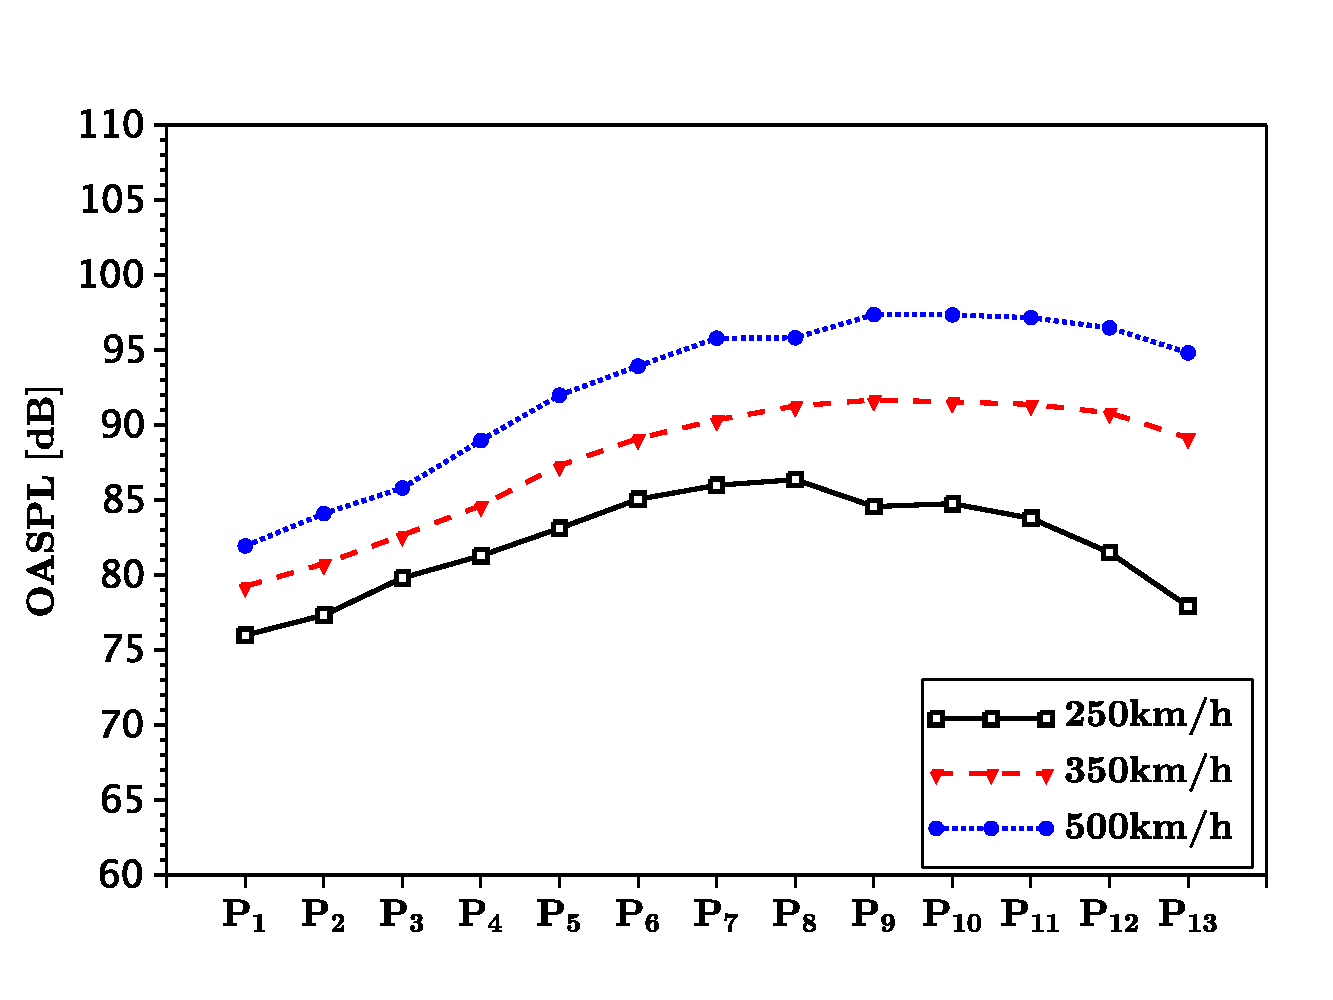
\includegraphics[width=\linewidth]{Figures/oaspl_c.pdf}
    \neusubfigcaption{fig:ch0-side-by-side-a}{工况一}
  \end{neusubfigure}
  \hfill
  \begin{neusubfigure}{0.49\linewidth}
    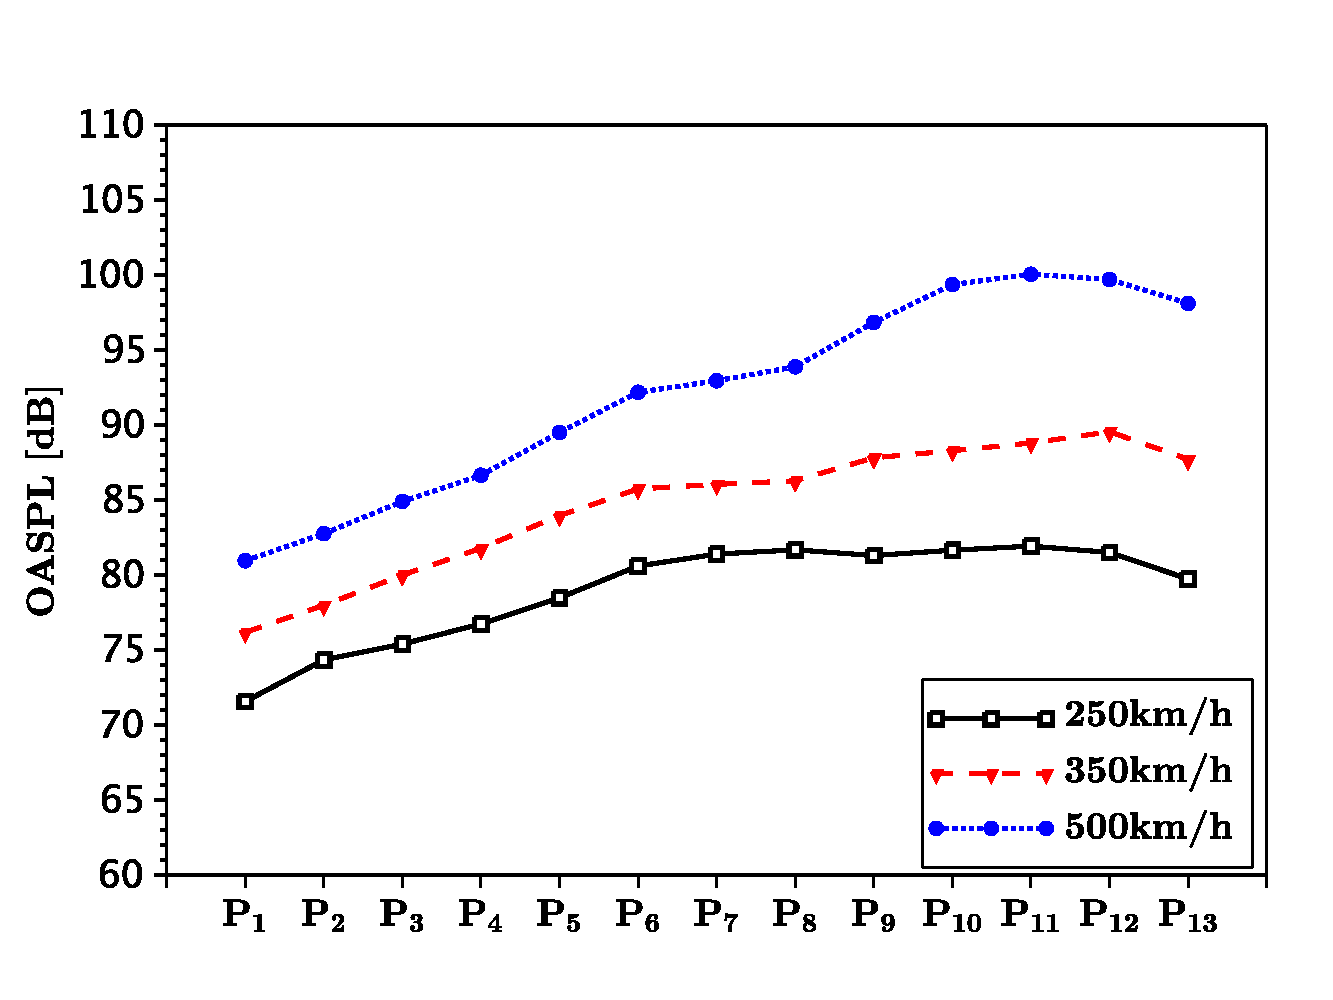
\includegraphics[width=\linewidth]{Figures/oaspl_d.pdf}
    \neusubfigcaption{fig:ch0-side-by-side-b}{工况二}
  \end{neusubfigure}
  \neufigcaption{fig:ch0-subfigures}{并列子图排版样例}{Example of Side-by-Side Subfigures}
\end{figure}

\neufigref{fig:ch0-subfigures} 使用 \texttt{neusubfigure} 完成并列子图排版。
其中 \neusubfigref{fig:ch0-side-by-side-a} 和 \neusubfigref{fig:ch0-side-by-side-b} 可分别引用到子图。
当两幅图共享一个总标题且需要分别引用时，可使用这种方式；如果每幅图需要完全独立的图号，建议拆成两个独立的 \texttt{figure} 环境。

\subsection{二乘二子图}
\begin{figure}[!htbp]
  \centering
  \begin{neusubfigure}{0.49\linewidth}
    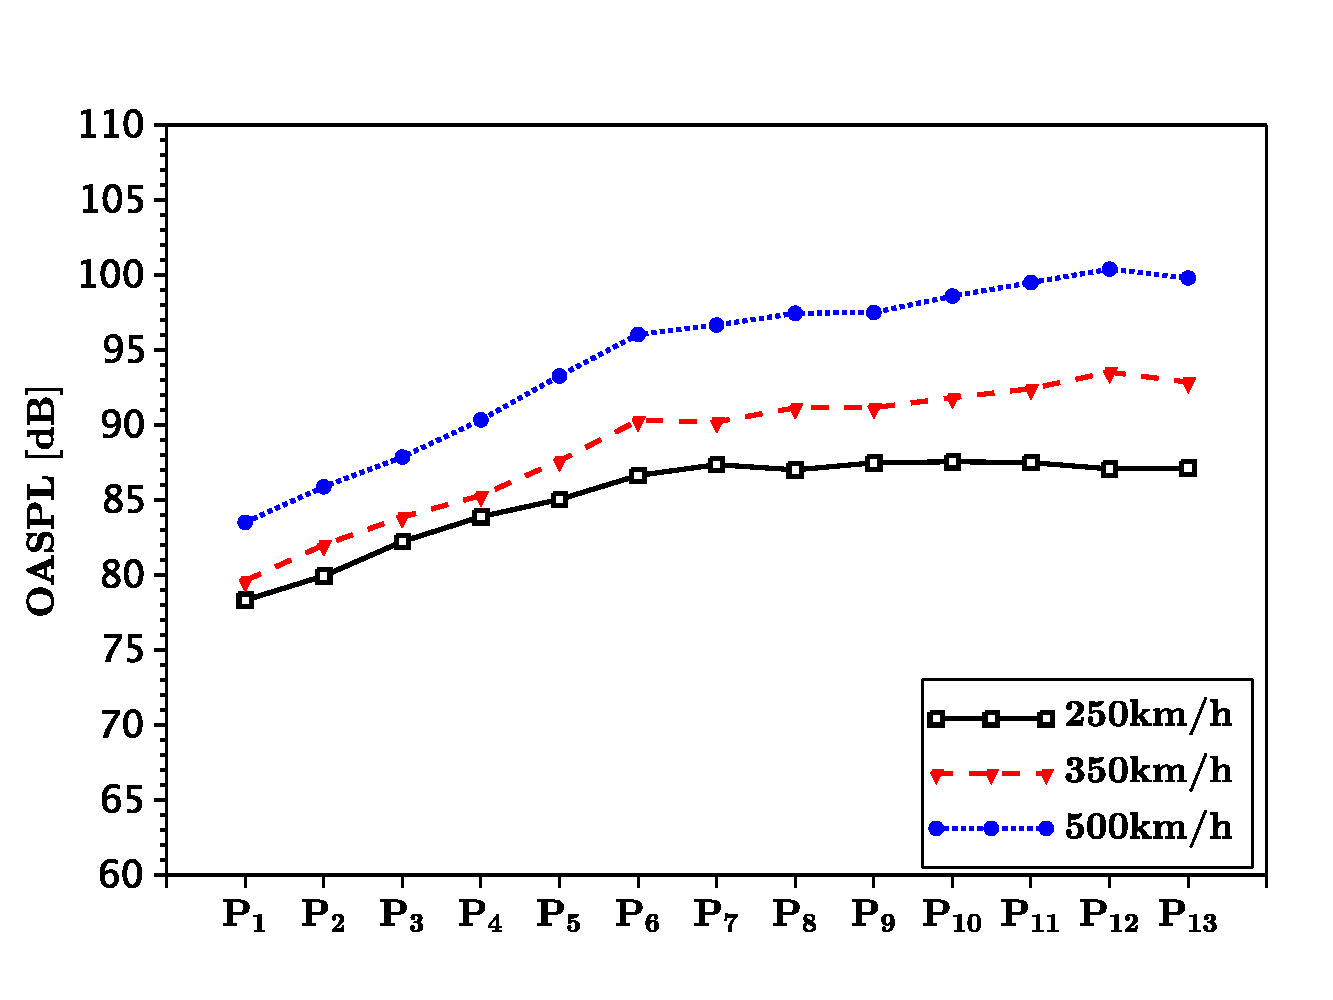
\includegraphics[width=\linewidth]{Figures/oaspl_a.pdf}
    \neusubfigcaption{fig:ch0-four-subfig-a}{工况一}
  \end{neusubfigure}
  \hfill
  \begin{neusubfigure}{0.49\linewidth}
    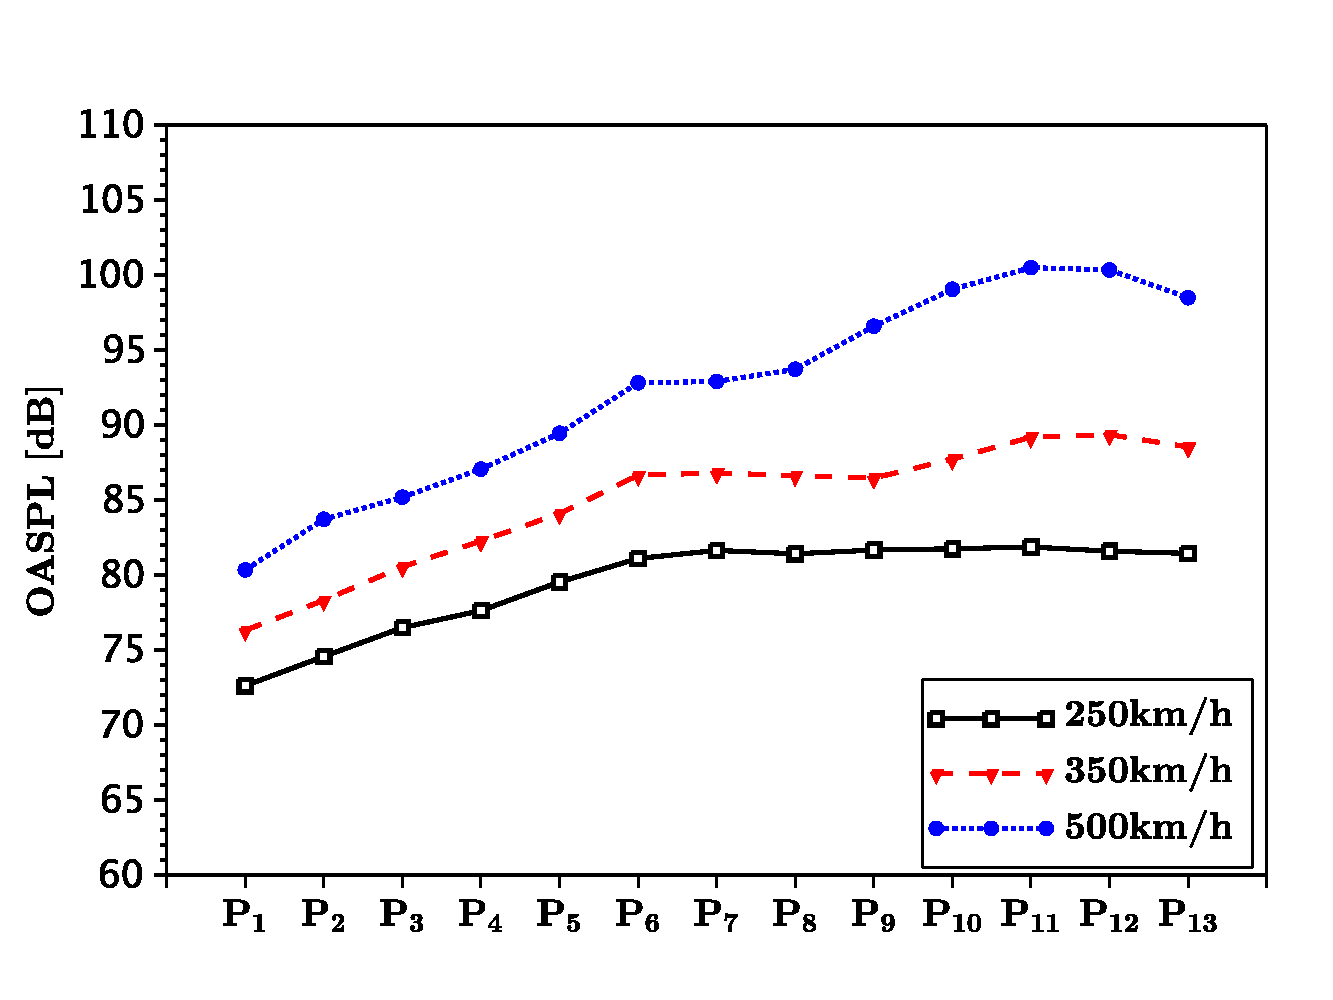
\includegraphics[width=\linewidth]{Figures/oaspl_b.pdf}
    \neusubfigcaption{fig:ch0-four-subfig-b}{工况二}
  \end{neusubfigure}
  \par\vspace{2bp}

  \begin{neusubfigure}{0.49\linewidth}
    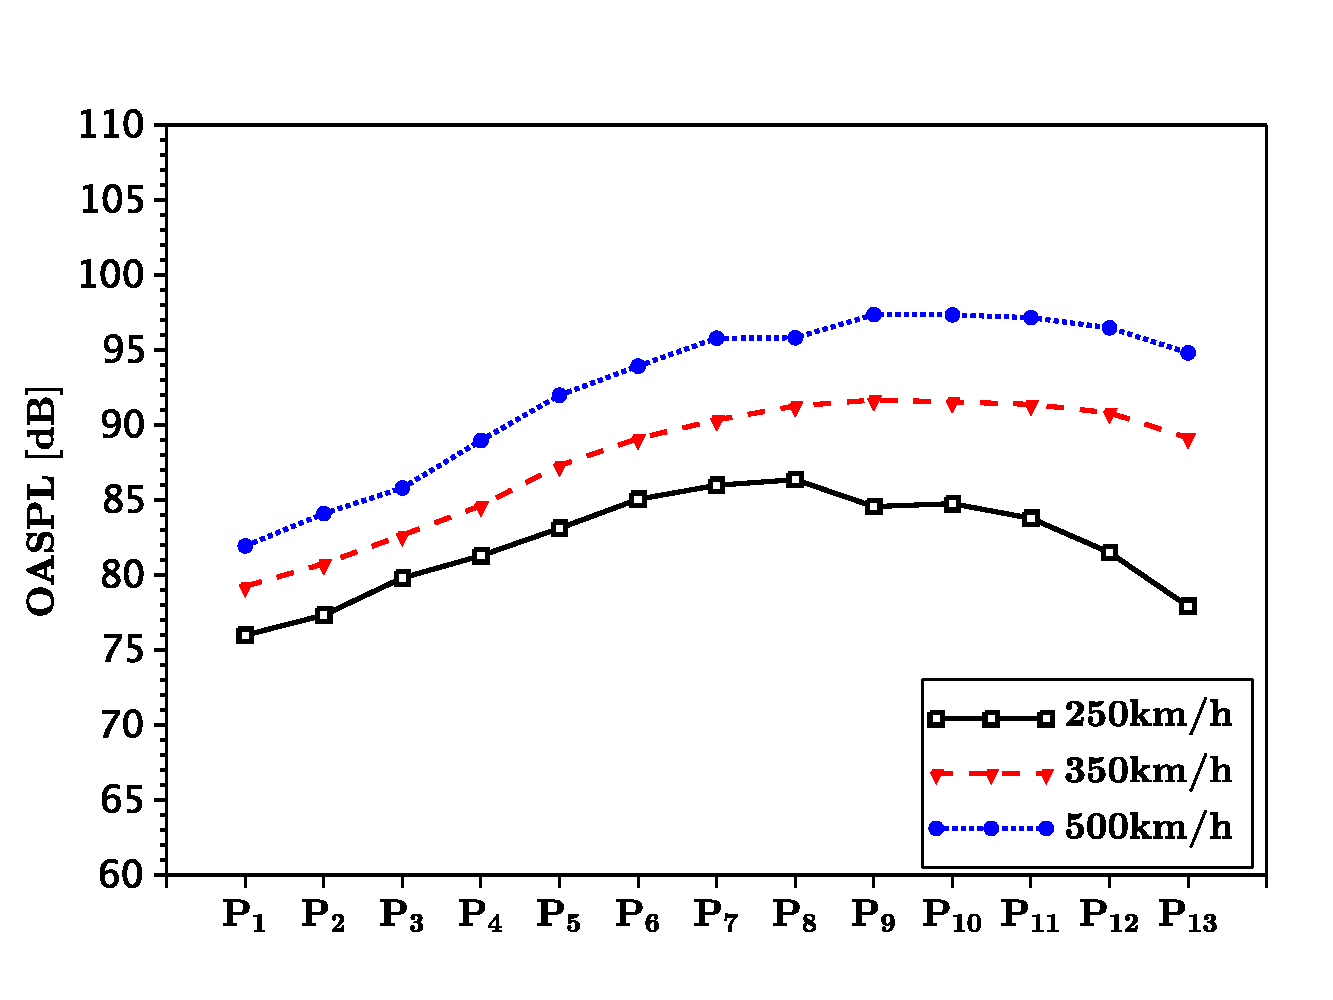
\includegraphics[width=\linewidth]{Figures/oaspl_c.pdf}
    \neusubfigcaption{fig:ch0-four-subfig-c}{工况三}
  \end{neusubfigure}
  \hfill
  \begin{neusubfigure}{0.49\linewidth}
    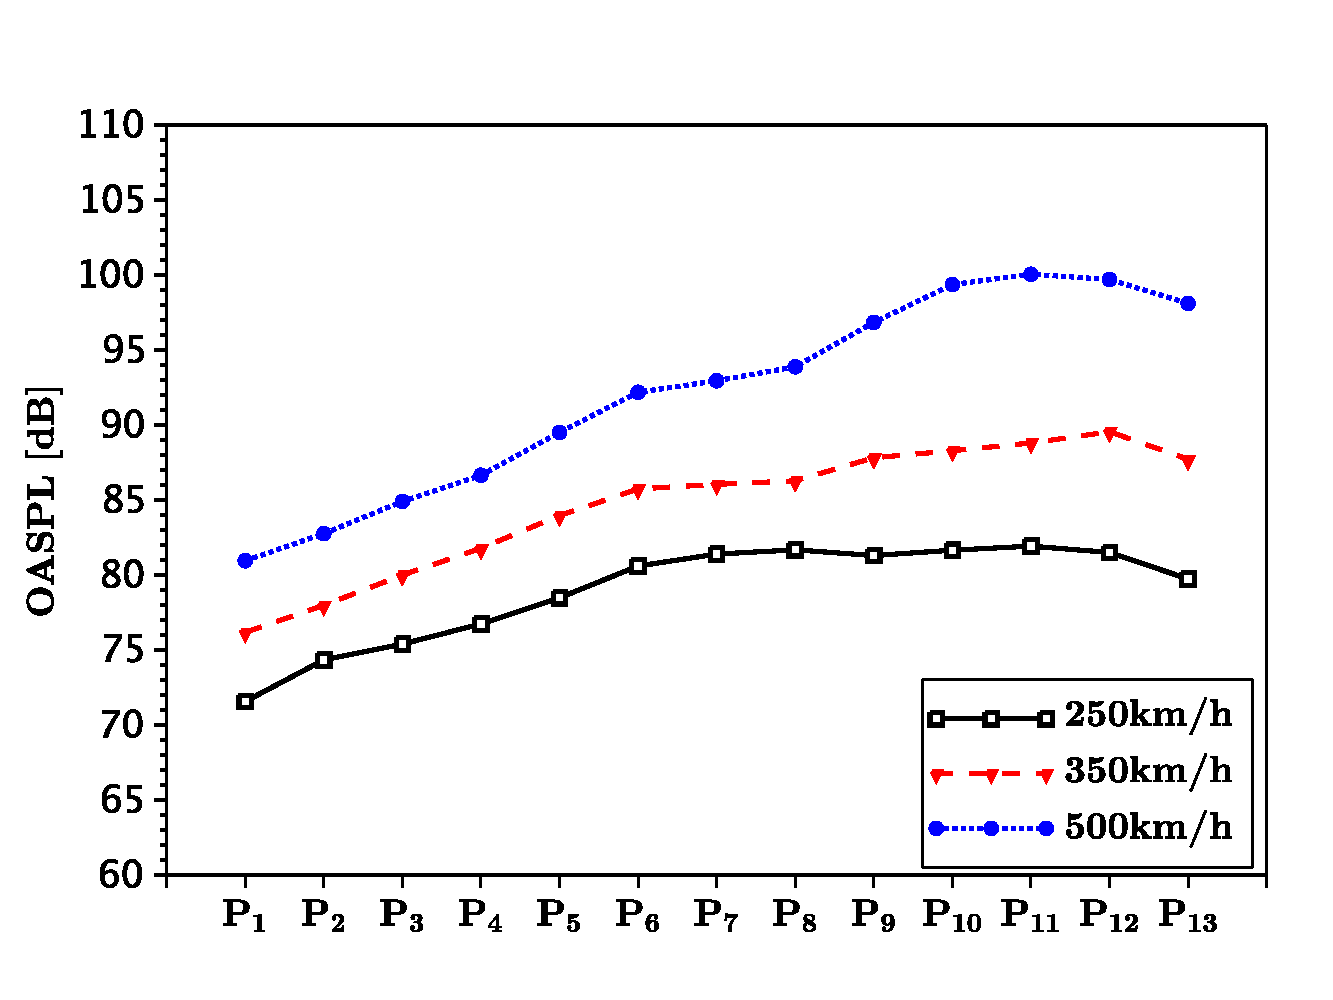
\includegraphics[width=\linewidth]{Figures/oaspl_d.pdf}
    \neusubfigcaption{fig:ch0-four-subfig-d}{工况四}
  \end{neusubfigure}
  \neufigcaption{fig:ch0-four-subfigures}{二乘二子图排版样例}{Example of Two-by-Two Subfigures}
\end{figure}

\neufigref{fig:ch0-four-subfigures} 展示了四幅子图的二乘二排布。
例如 \neusubfigref{fig:ch0-four-subfig-a} 至 \neusubfigref{fig:ch0-four-subfig-d} 可分别引用到四个子图。
排版时建议注意以下几点：
\begin{itemize}
  \item 子图宽度通常可取 \verb|0.48\linewidth| 至 \verb|0.49\linewidth|。
  \item 每行两个子图之间使用 \verb|\hfill| 自动拉开横向间距。
  \item 两行之间可用少量 \verb|\par\vspace| 控制垂直间距。
\end{itemize}

\section{表格排版}

本模板提供 \verb|\neutabcaption{label}{中文题名}{English title}| 用于生成中英文表题。
表题应置于表格上方，正文中使用 \verb|\neutabref{label}| 引用。
表格同样建议使用 \verb|[!htbp]|。如果表格过高导致页底空白，优先考虑缩小字号、调整列宽、拆分表格或使用跨页表格，而不是强制分页。

\subsection{三线表}

\begin{table}[!htbp]
  \centering
  \neutabcaption{tab:ch0-booktabs}{三线表样例}{Example of a Three-Line Table}
  \begin{tabular}{lccc}
    \toprule
    方法       & 准确率（\%）       & 召回率（\%）       & F1 值           \\
    \midrule
    Baseline & 85.2          & 84.1          & 0.846          \\
    Method A & 89.7          & 88.9          & 0.893          \\
    Proposed & \textbf{92.1} & \textbf{91.5} & \textbf{0.918} \\
    \bottomrule
  \end{tabular}
\end{table}

\neutabref{tab:ch0-booktabs} 展示了推荐的三线表格式。
论文中应尽量避免过多竖线，以保持表格简洁。

\subsection{复杂表格}
\begin{table}[!htbp]
  \centering
  \neutabcaption{tab:ch0-complex}{合并单元格与自动换行表格样例}{Example of Merged Cells and Auto-Wrapping Columns}
  \begin{tabularx}{\textwidth}{llXc}
    \toprule
    类别                  & 指标  & 说明                               & 是否必需 \\
    \midrule
    \multirow{2}{*}{图形} & 分辨率 & 位图图片应保证在最终 PDF 中清晰可辨。            & 是    \\
                        & 题名  & 图题使用中英文双语标题，并位于图片下方。             & 是    \\
    \midrule
    \multirow{2}{*}{表格} & 宽度  & 宽表格可使用 \texttt{tabularx} 自动分配列宽。 & 否    \\
                        & 表注  & 表内说明应简明，必要时可在正文中解释。              & 否    \\
    \bottomrule
  \end{tabularx}
\end{table}

\neutabref{tab:ch0-complex} 同时展示了 \verb|\multirow|、\verb|\makecell| 可配合使用的复杂表格场景。
若单元格内容较长，优先使用 \texttt{tabularx} 或 \texttt{p\{...\}} 列类型控制宽度。

\section{公式排版}

公式应使用标准数学环境，并通过 \verb|\label| 设置标签。
引用公式时建议使用模板提供的 \verb|\neueqref{label}|。

\subsection{单行公式}
以分类任务中的交叉熵损失为例，可写为
\begin{equation}
  \mathcal{L}(\theta)
  = - \frac{1}{N}\sum_{i=1}^{N}\sum_{k=1}^{K} y_{ik}\log p_{ik}
  \label{eq:ch0-loss}
\end{equation}

如 \neueqref{eq:ch0-loss} 所示，带编号公式适合放置正文中需要引用的重要定义。

\subsection{多行公式}
循环模型中的状态更新和输出计算可写为
\begin{align}
  h_t       & = \sigma(W_x x_t + W_h h_{t-1} + b), \label{eq:ch0-state} \\
  \hat{y}_t & = \operatorname{softmax}(W_o h_t). \label{eq:ch0-output}
\end{align}

\neueqref{eq:ch0-state} 和 \neueqref{eq:ch0-output} 展示了多行公式的编号方式。
如果多行推导只需要一个编号，可使用 \texttt{aligned} 放在 \texttt{equation} 环境内部。

\subsection{分段函数与矩阵}
分段函数和矩阵经常同时出现在数学定义中，例如
\begin{equation}
  g(x)=
  \begin{cases}
    0, & x < 0,       \\
    x, & 0 \le x < 1, \\
    1, & x \ge 1,
  \end{cases}
  \qquad
  A =
  \begin{bmatrix}
    1 & 0 & 0 \\
    0 & 1 & 0 \\
    0 & 0 & 1
  \end{bmatrix}.
  \label{eq:ch0-piecewise}
\end{equation}

\neueqref{eq:ch0-piecewise} 展示了分段函数和矩阵的常见写法。

\section{算法伪代码}

计算机类论文常需要给出算法步骤。本文档在 \texttt{main.tex} 中加载了 \texttt{algorithm} 和 \texttt{algorithmic} 宏包，可以直接使用如下环境。

\begin{algorithm}[!htbp]
  \caption{样例训练流程}
  \label{alg:ch0-training}
  \begin{algorithmic}[1]
    \REQUIRE Training set $\mathcal{D}$, learning rate $\eta$, maximum epoch $T$
    \ENSURE Model parameters $\theta$
    \STATE Initialize parameters $\theta$
    \FOR{$t = 1$ to $T$}
    \STATE Sample a mini-batch $\mathcal{B}$ from $\mathcal{D}$
    \STATE Compute loss $\mathcal{L}(\theta)$ by \neueqref{eq:ch0-loss}
    \STATE Update $\theta \leftarrow \theta - \eta \nabla_{\theta}\mathcal{L}(\theta)$
    \ENDFOR
    \RETURN $\theta$
  \end{algorithmic}
\end{algorithm}

算法~\ref{alg:ch0-training} 展示了带行号的伪代码。
若需要中文关键字，可在导言区重定义相应命令。

\section{引用、链接与交叉引用}

参考文献引用可使用两种模板命令：
\begin{itemize}
  \item 上标引用使用 \verb|\upcite{key}|，适合放在句末，例如已有研究讨论了神经网络轻量化问题\upcite{guo_2023_research}。
  \item 正文引用使用 \verb|\inlinecite{key}|，适合作为句子成分，例如文献 \inlinecite{thakkar_2018_performance} 给出了系统性能评测案例。
\end{itemize}
多篇文献可写在同一条引用命令中，例如区块链平台相关研究\upcite{zheng_2019_nutbaas,thakkar_2018_performance}。

交叉引用建议统一使用模板命令：
\begin{itemize}
  \item 图引用：\verb|\neufigref{fig:ch0-pdf}|，效果为 \neufigref{fig:ch0-pdf}。
  \item 子图引用：\verb|\neusubfigref{fig:ch0-four-subfig-a}|，效果为 \neusubfigref{fig:ch0-four-subfig-a}。
  \item 表引用：\verb|\neutabref{tab:ch0-complex}|，效果为 \neutabref{tab:ch0-complex}。
  \item 公式引用：\verb|\neueqref{eq:ch0-loss}|，效果为 \neueqref{eq:ch0-loss}。
  \item 算法引用：当前模板未单独封装算法引用命令，可写作“算法~\ref{alg:ch0-training}”。
\end{itemize}
模板提供的公开命令和环境可参考 \texttt{README.md} 中的“模板命令说明”一节。
|，并从第~\ref{chap:introduction}~章开始组织正式内容。

\section{章节层级与正文段落}

论文正文通常从一级标题开始组织内容，一级标题使用 \verb|\chapter|，二级标题使用 \verb|\section|，三级标题使用 \verb|\subsection|。
本模板会自动设置章标题、节标题、页眉、页码和目录格式，作者只需要关注正文内容。
正文段落首行缩进、行距和中英文字体均由模板统一控制，一般不需要在正文中手动设置字号、字体或段间距。

中文正文可以直接书写；英文术语建议在首次出现时给出全称，例如自然语言处理（Natural Language Processing, NLP）。
行内公式可以写作 $E=mc^2$，行内代码或命令可以使用 \verb|\verb|，例如 \verb|%!TEX root = ./main.tex
\chapter{论文格式样例与模板验证}

本章作为模板的集中样例章，用于快速检查正文中常见排版元素的显示效果。
样例覆盖章节层级、正文段落、列表、脚注、图、表、公式、算法、交叉引用和参考文献引用等内容。
编写正式论文时，可以保留本章作为排版对照；定稿前可在 \texttt{main.tex} 中删除或注释 \verb|%!TEX root = ./main.tex
\chapter{论文格式样例与模板验证}

本章作为模板的集中样例章，用于快速检查正文中常见排版元素的显示效果。
样例覆盖章节层级、正文段落、列表、脚注、图、表、公式、算法、交叉引用和参考文献引用等内容。
编写正式论文时，可以保留本章作为排版对照；定稿前可在 \texttt{main.tex} 中删除或注释 \verb|\input{chapter0-guide}|，并从第~\ref{chap:introduction}~章开始组织正式内容。

\section{章节层级与正文段落}

论文正文通常从一级标题开始组织内容，一级标题使用 \verb|\chapter|，二级标题使用 \verb|\section|，三级标题使用 \verb|\subsection|。
本模板会自动设置章标题、节标题、页眉、页码和目录格式，作者只需要关注正文内容。
正文段落首行缩进、行距和中英文字体均由模板统一控制，一般不需要在正文中手动设置字号、字体或段间距。

中文正文可以直接书写；英文术语建议在首次出现时给出全称，例如自然语言处理（Natural Language Processing, NLP）。
行内公式可以写作 $E=mc^2$，行内代码或命令可以使用 \verb|\verb|，例如 \verb|\input{chapter0-guide}|。
脚注示例如此处所示\footnote{脚注用于补充说明，不宜放置过长的正文内容。}。
若某页因图表浮动或分页规则没有排满，脚注可能跟随正文排版区而显得略高，这是正常的 LaTeX 页面构建结果。

\subsection{字体、字号与强调}

模板预定义了常用中文字体命令。正式论文中通常不需要手动切换字体；只有在展示样式、术语强调或特殊说明时才建议使用。
当前模板已经为默认宋体和 \verb|\song| 字族配置伪粗体，因此 \verb|\textbf| 或 \verb|\bfseries| 可以用于中文局部强调。
需要注意的是，中文加粗应克制使用；标题层级、术语定义或表格重点值可以适当加粗，大段正文不建议整体加粗。
如果需要更明显的标题式强调，可使用黑体或调整标题层级；如果只是普通正文重点，优先使用 \verb|\textbf|。

\begin{table}[!htbp]
  \centering
  \neutabcaption{tab:ch0-fonts}{字体与强调样例}{Examples of Fonts and Emphasis}
  \begin{tabular}{lll}
    \toprule
    命令             & 显示效果                         & 使用建议       \\
    \midrule
    \verb|\song|   & {\song 宋体文字示例}               & 正文默认字体     \\
    \verb|\textbf| & \textbf{加粗文字示例}              & 局部强调、表格重点值 \\
    \verb|\hei|    & {\hei 黑体文字示例}                & 标题或较强强调场景  \\
    \verb|\kai|    & {\kai 楷体文字示例}                & 摘要、题签或引用语  \\
    \verb|\fs|     & {\fs 仿宋文字示例}                 & 特殊文书类内容    \\
    \verb|\textit| & \textit{Italic text example} & 英文斜体或变量说明  \\
    \bottomrule
  \end{tabular}
\end{table}

\subsection{列表环境}

无序列表适合列出并列事项：
\begin{itemize}
  \item 图题位于图下方，表题位于表上方。
  \item 图表应使用中英文双语标题。
  \item 公式、图、表、算法均应使用标签进行交叉引用。
\end{itemize}

有序列表适合描述步骤：
\begin{enumerate}
  \item 在 \texttt{main.tex} 中填写论文元信息。
  \item 在各章文件中撰写正文内容。
  \item 使用 \texttt{latexmk -xelatex main.tex} 完成编译。
\end{enumerate}

\section{图形排版}

本模板提供 \verb|\neufigcaption{label}{中文题名}{English title}| 用于生成中英文图题。
图题应置于图形下方，正文中使用 \verb|\neufigref{label}| 引用。
图形建议使用 \verb|[!htbp]| 浮动参数，让 LaTeX 在当前位置、页顶、页底或浮动页中选择较合适的位置；除非必须固定位置，否则不建议使用 \verb|[H]|。

\subsection{外部图片}
\begin{figure}[!htbp]
  \centering
  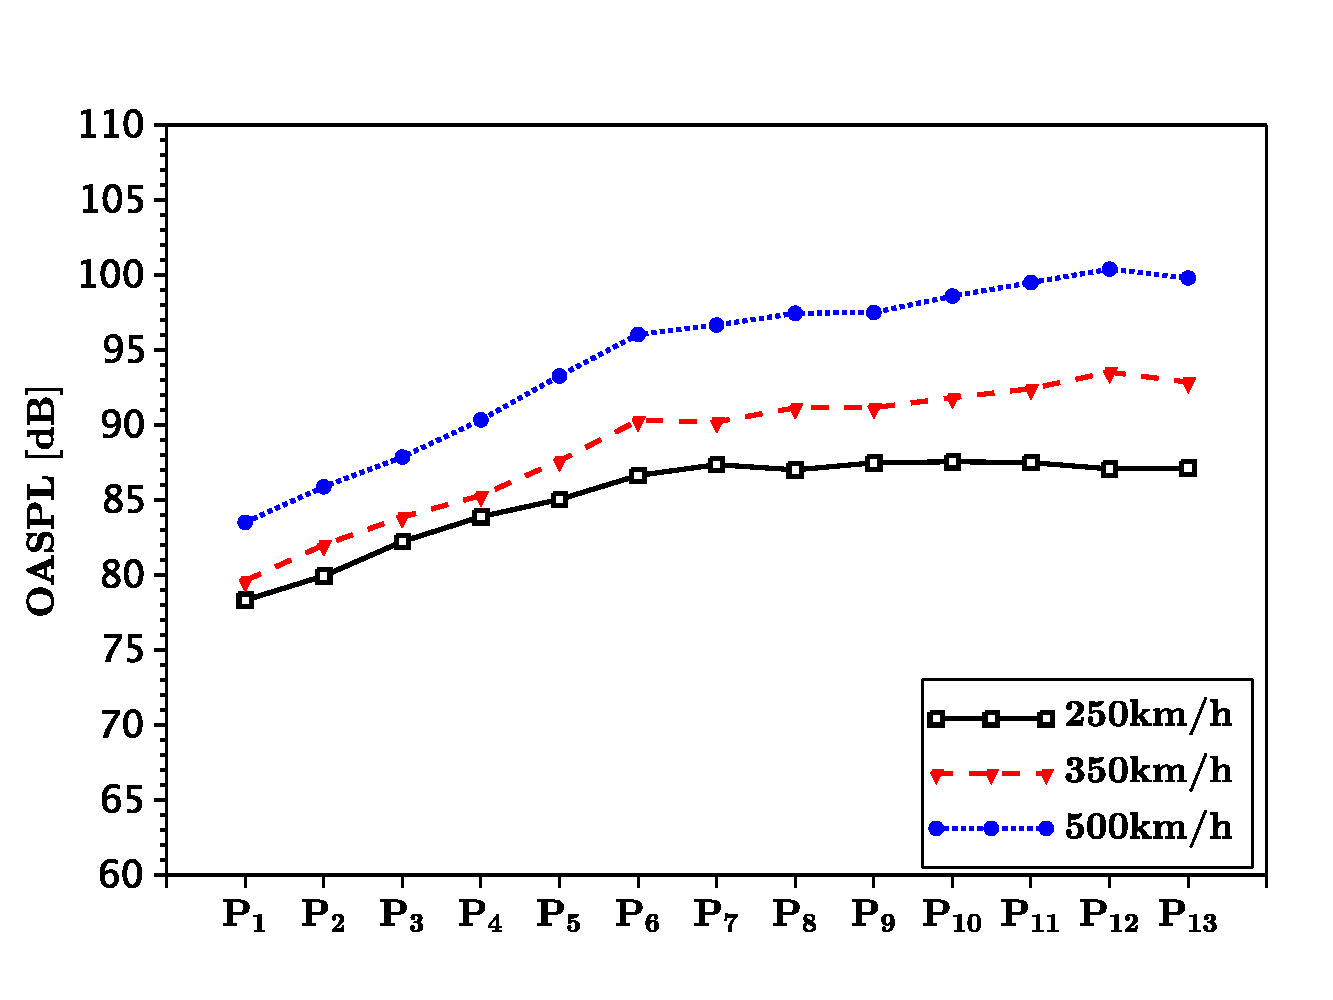
\includegraphics[width=0.55\textwidth]{Figures/oaspl_a.pdf}
  \neufigcaption{fig:ch0-cover}{外部图片插入样例}{Example of Including an External Image}
\end{figure}

\neufigref{fig:ch0-cover} 展示了通过 \verb|\includegraphics| 插入图片文件的方式。
正式论文中建议将图片统一放入 \texttt{Figures} 目录，并使用相对路径引用。

\subsection{PDF 或位图图片}
\begin{figure}[!htbp]
  \centering
  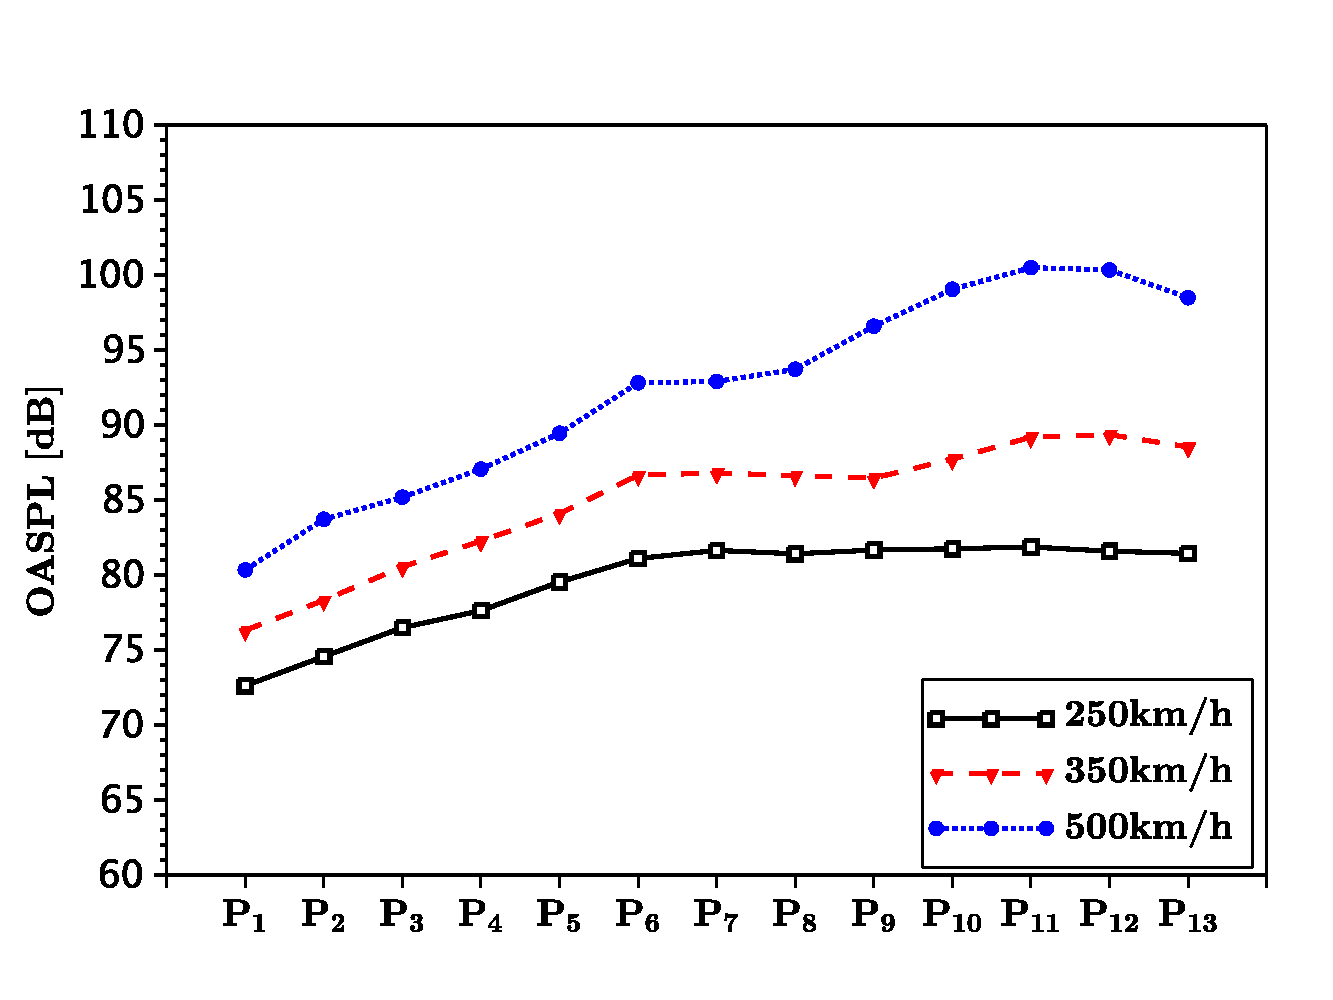
\includegraphics[width=0.55\textwidth]{Figures/oaspl_b.pdf}
  \neufigcaption{fig:ch0-pdf}{PDF 图片插入样例}{Example of Including a PDF Figure}
\end{figure}

PDF、PNG、JPG 等常见图片格式均可通过 \verb|\includegraphics| 插入。
若图片由绘图软件或数据分析程序导出，建议优先使用 PDF 格式以保持较清晰的显示效果。

\subsection{并列图片}
\begin{figure}[!htbp]
  \centering
  \begin{minipage}[t]{0.49\linewidth}
    \centering
    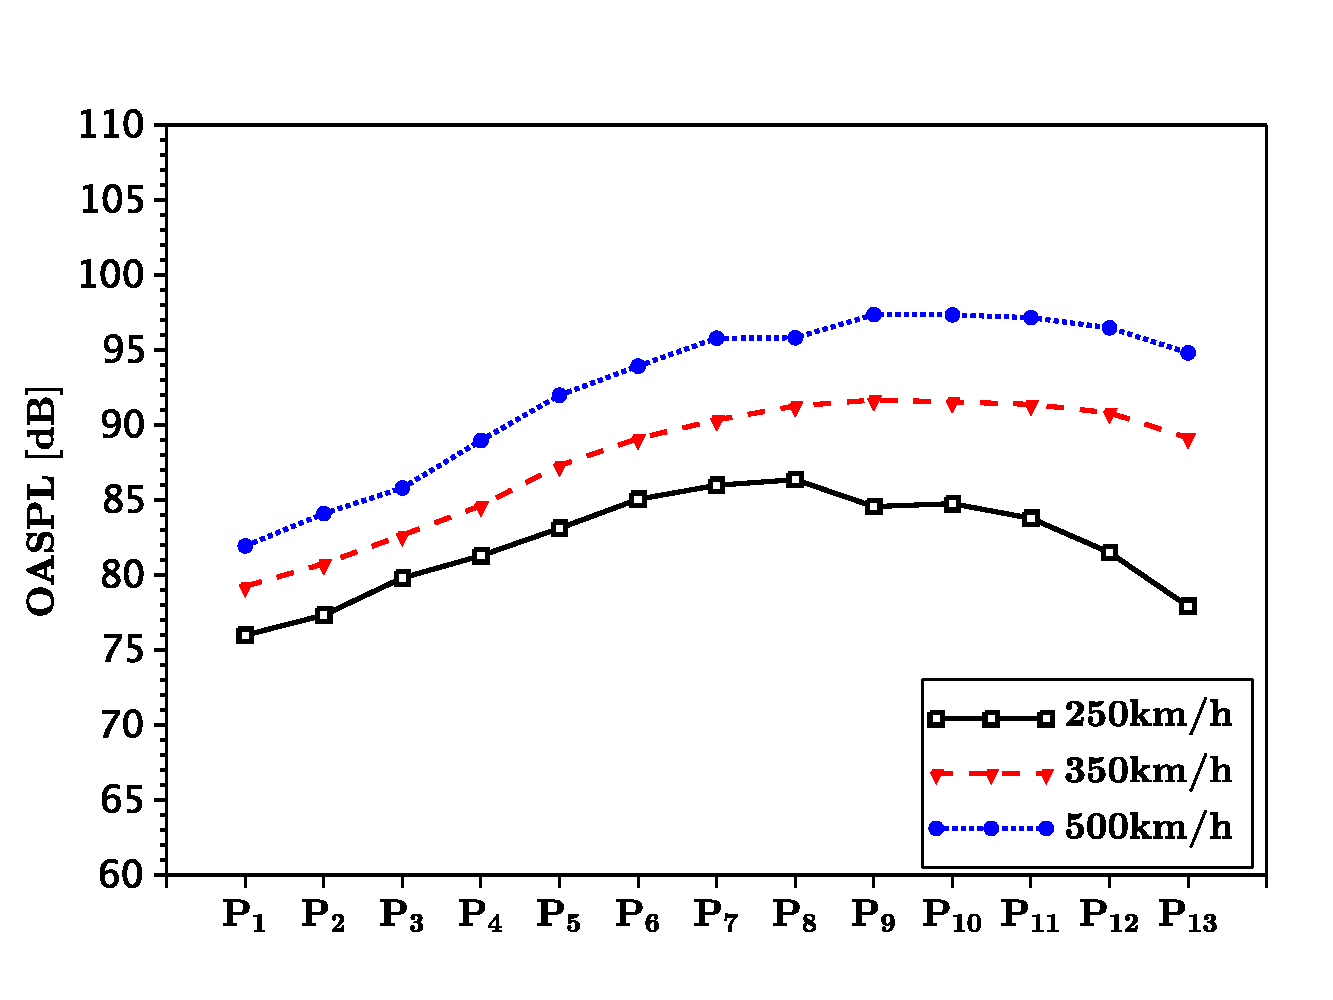
\includegraphics[width=\linewidth]{Figures/oaspl_c.pdf}
  \end{minipage}
  \hfill
  \begin{minipage}[t]{0.49\linewidth}
    \centering
    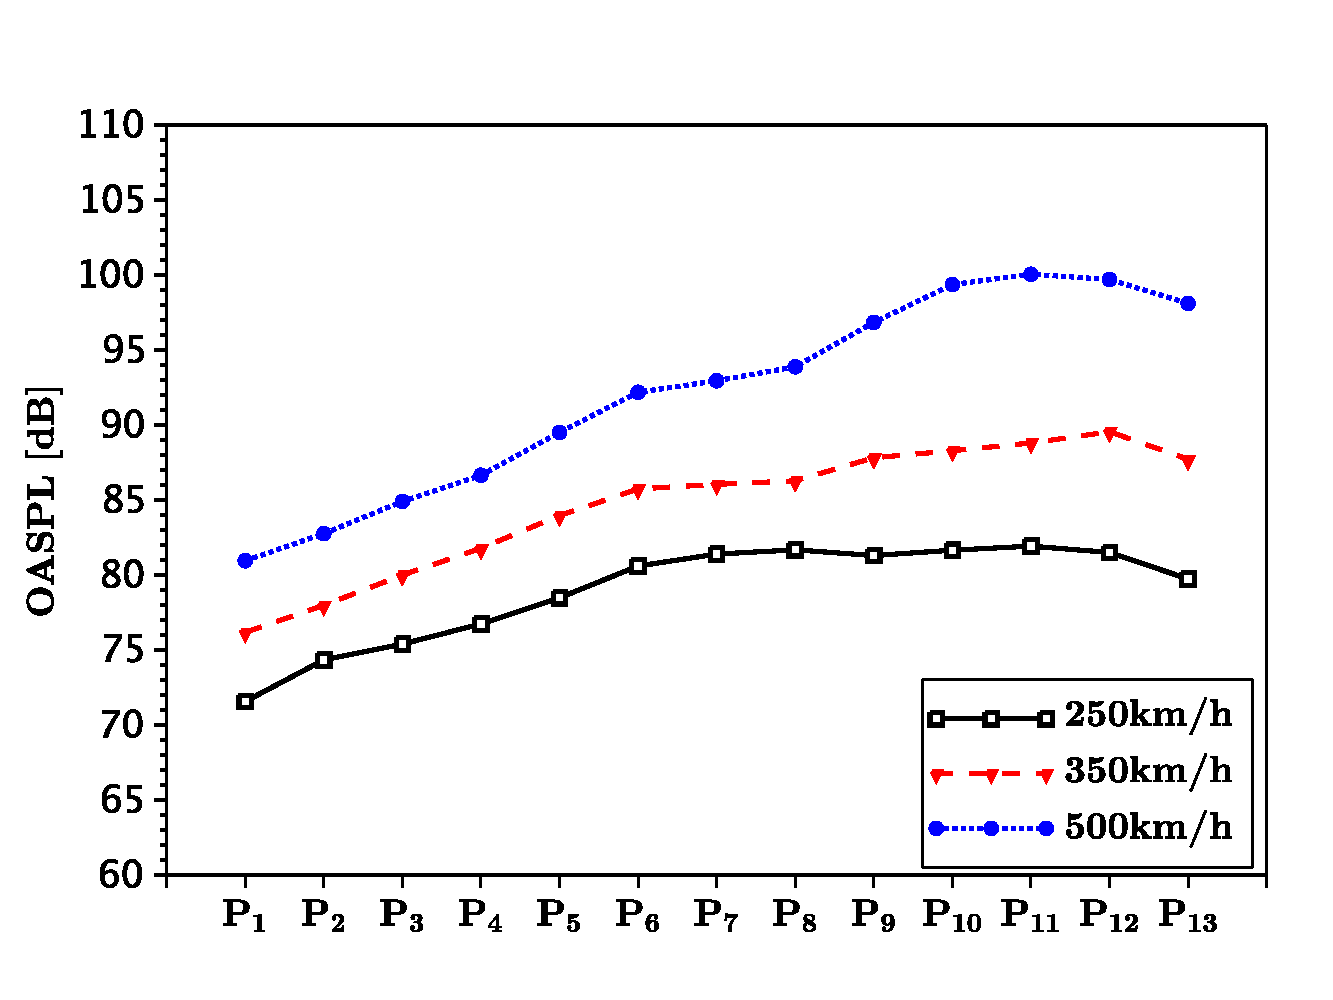
\includegraphics[width=\linewidth]{Figures/oaspl_d.pdf}
  \end{minipage}
  \neufigcaption{fig:ch0-side-by-side}{普通并列图形排版样例}{Example of Side-by-Side Figures}
\end{figure}

\neufigref{fig:ch0-side-by-side} 使用 \texttt{minipage} 完成普通并列排版。
当两幅图共享一个总标题且不需要分别引用时，可使用这种方式。

\subsection{并列子图}
\begin{figure}[!htbp]
  \centering
  \begin{neusubfigure}{0.49\linewidth}
    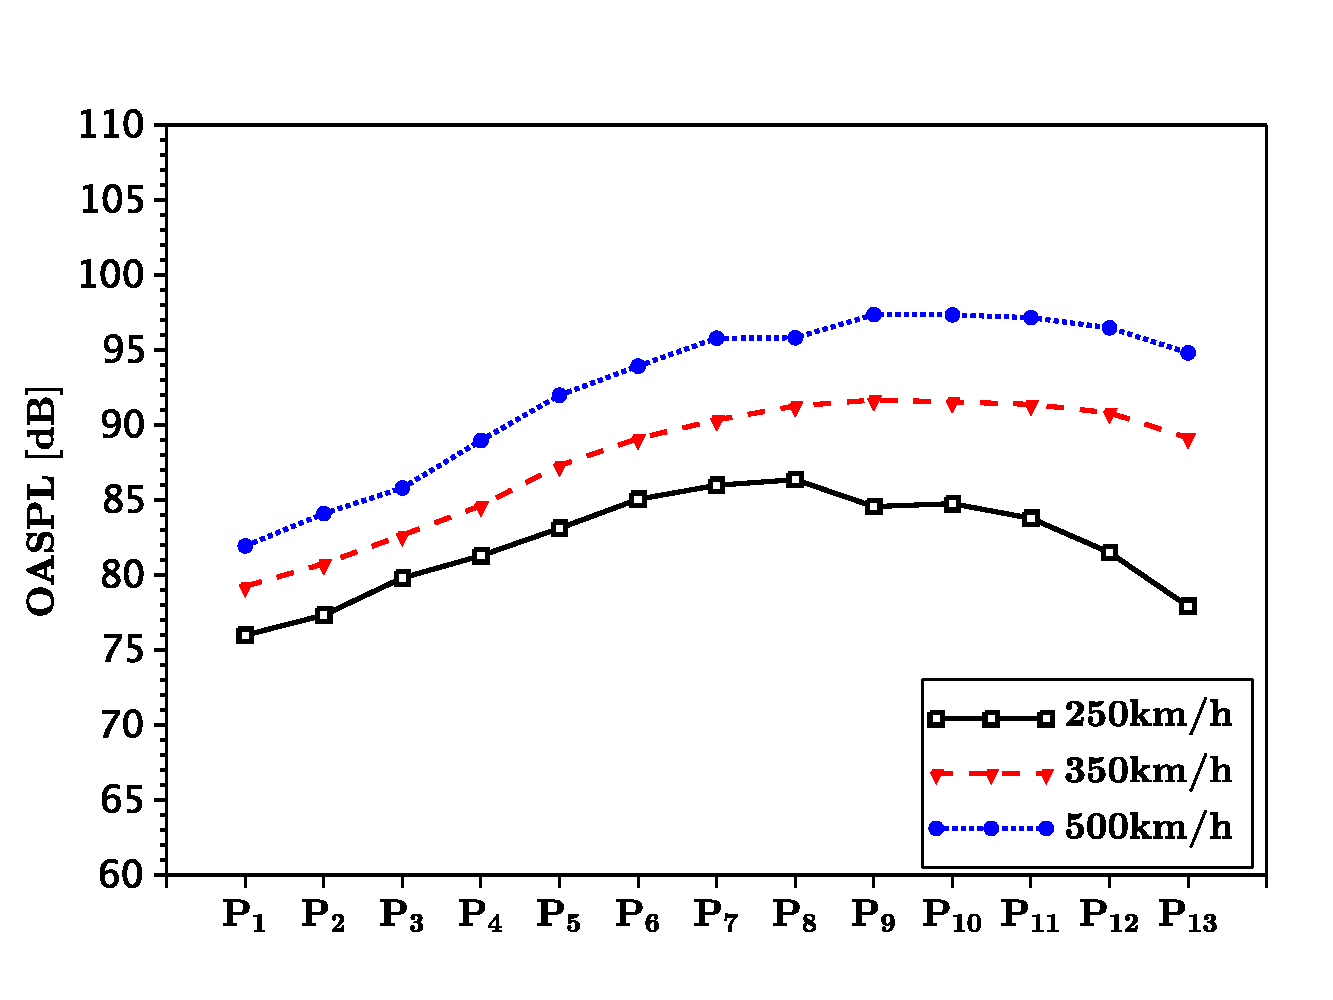
\includegraphics[width=\linewidth]{Figures/oaspl_c.pdf}
    \neusubfigcaption{fig:ch0-side-by-side-a}{工况一}
  \end{neusubfigure}
  \hfill
  \begin{neusubfigure}{0.49\linewidth}
    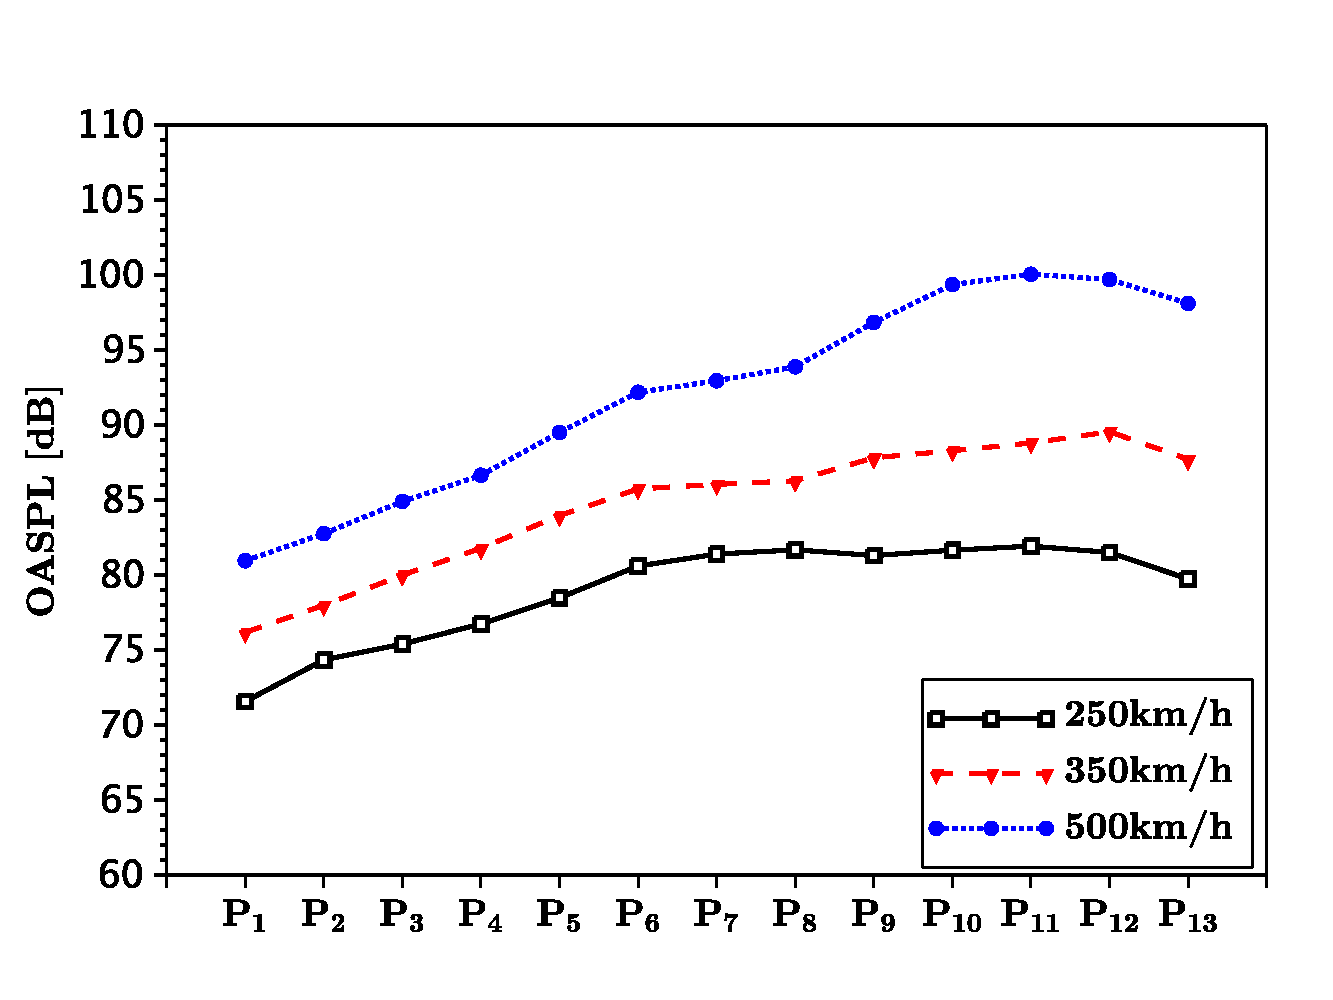
\includegraphics[width=\linewidth]{Figures/oaspl_d.pdf}
    \neusubfigcaption{fig:ch0-side-by-side-b}{工况二}
  \end{neusubfigure}
  \neufigcaption{fig:ch0-subfigures}{并列子图排版样例}{Example of Side-by-Side Subfigures}
\end{figure}

\neufigref{fig:ch0-subfigures} 使用 \texttt{neusubfigure} 完成并列子图排版。
其中 \neusubfigref{fig:ch0-side-by-side-a} 和 \neusubfigref{fig:ch0-side-by-side-b} 可分别引用到子图。
当两幅图共享一个总标题且需要分别引用时，可使用这种方式；如果每幅图需要完全独立的图号，建议拆成两个独立的 \texttt{figure} 环境。

\subsection{二乘二子图}
\begin{figure}[!htbp]
  \centering
  \begin{neusubfigure}{0.49\linewidth}
    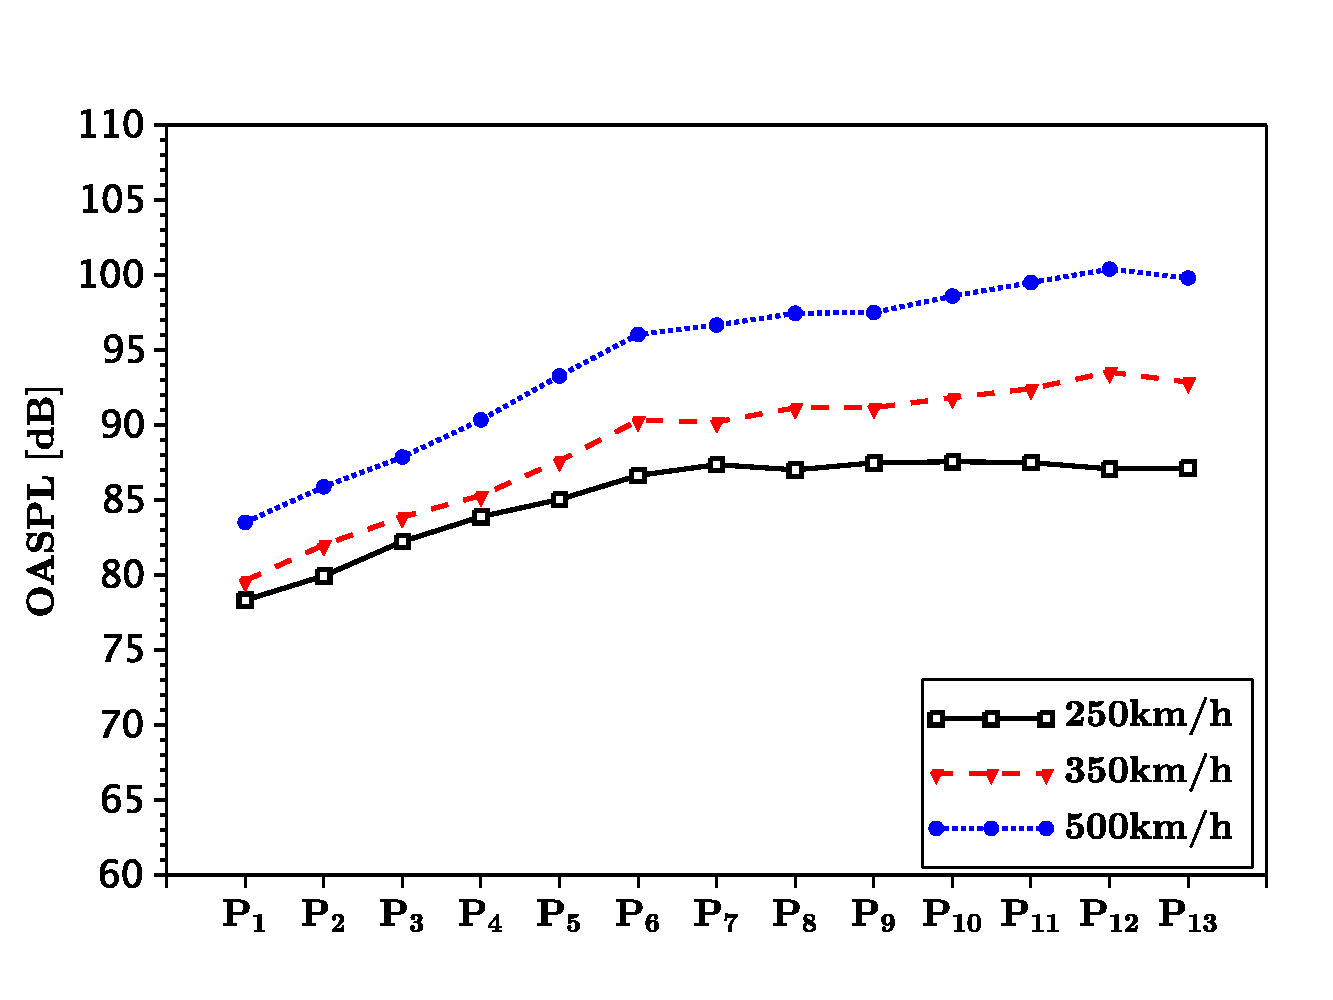
\includegraphics[width=\linewidth]{Figures/oaspl_a.pdf}
    \neusubfigcaption{fig:ch0-four-subfig-a}{工况一}
  \end{neusubfigure}
  \hfill
  \begin{neusubfigure}{0.49\linewidth}
    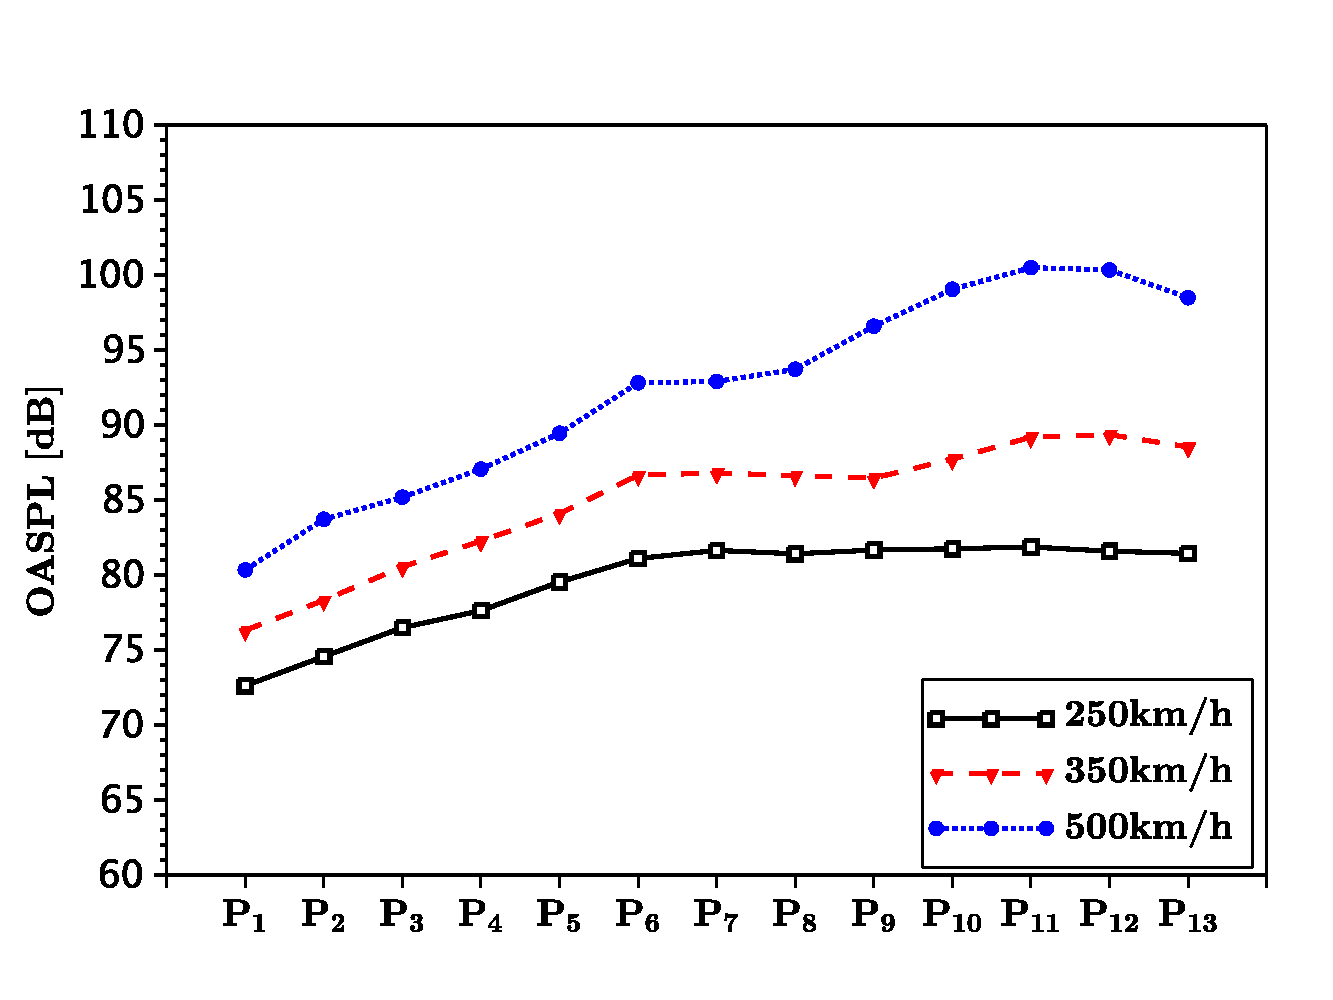
\includegraphics[width=\linewidth]{Figures/oaspl_b.pdf}
    \neusubfigcaption{fig:ch0-four-subfig-b}{工况二}
  \end{neusubfigure}
  \par\vspace{2bp}

  \begin{neusubfigure}{0.49\linewidth}
    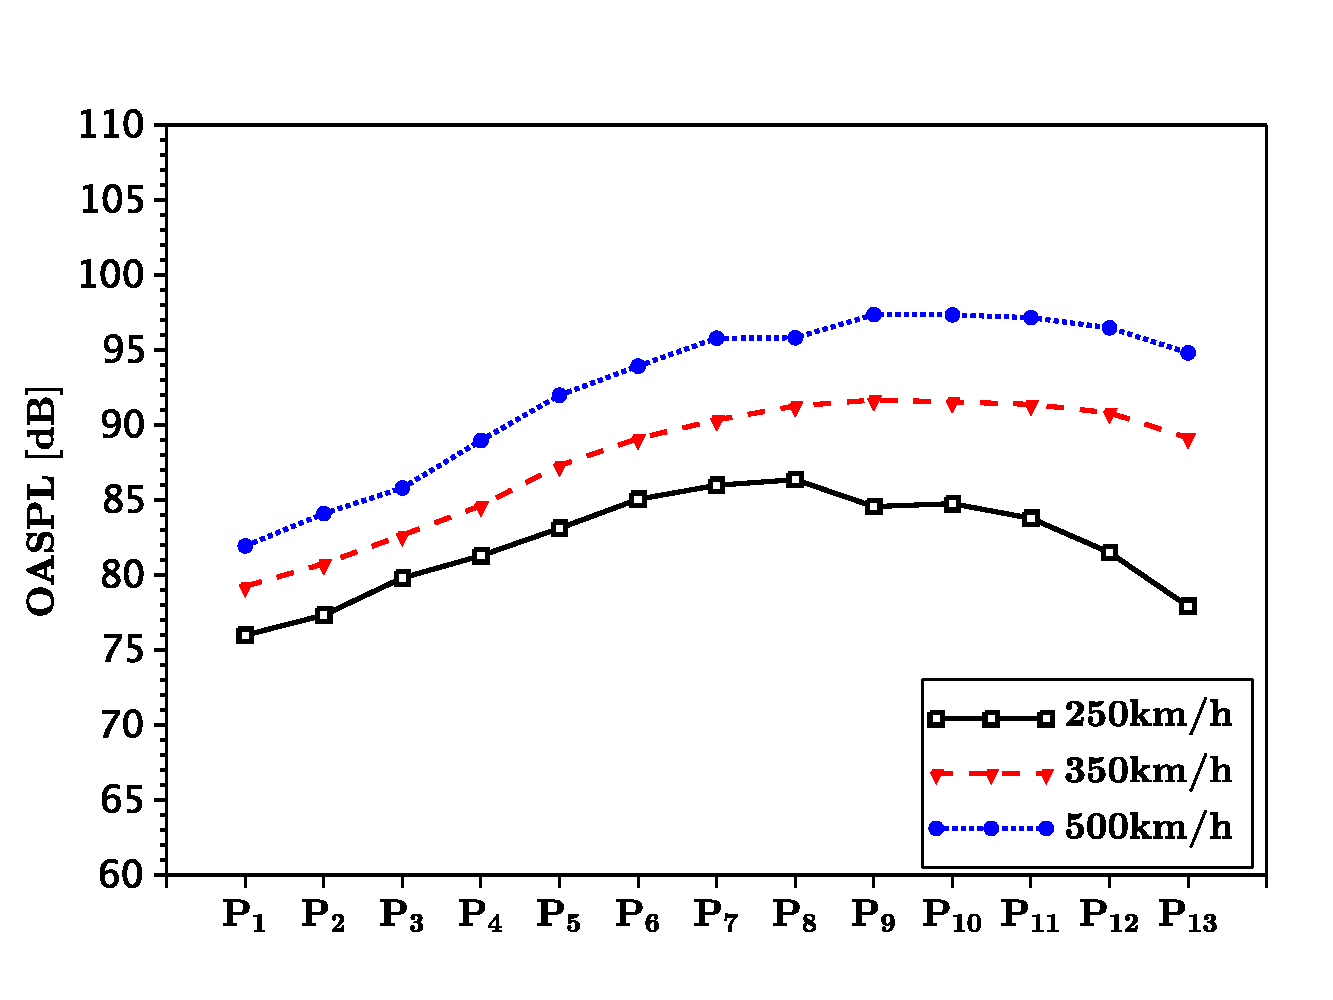
\includegraphics[width=\linewidth]{Figures/oaspl_c.pdf}
    \neusubfigcaption{fig:ch0-four-subfig-c}{工况三}
  \end{neusubfigure}
  \hfill
  \begin{neusubfigure}{0.49\linewidth}
    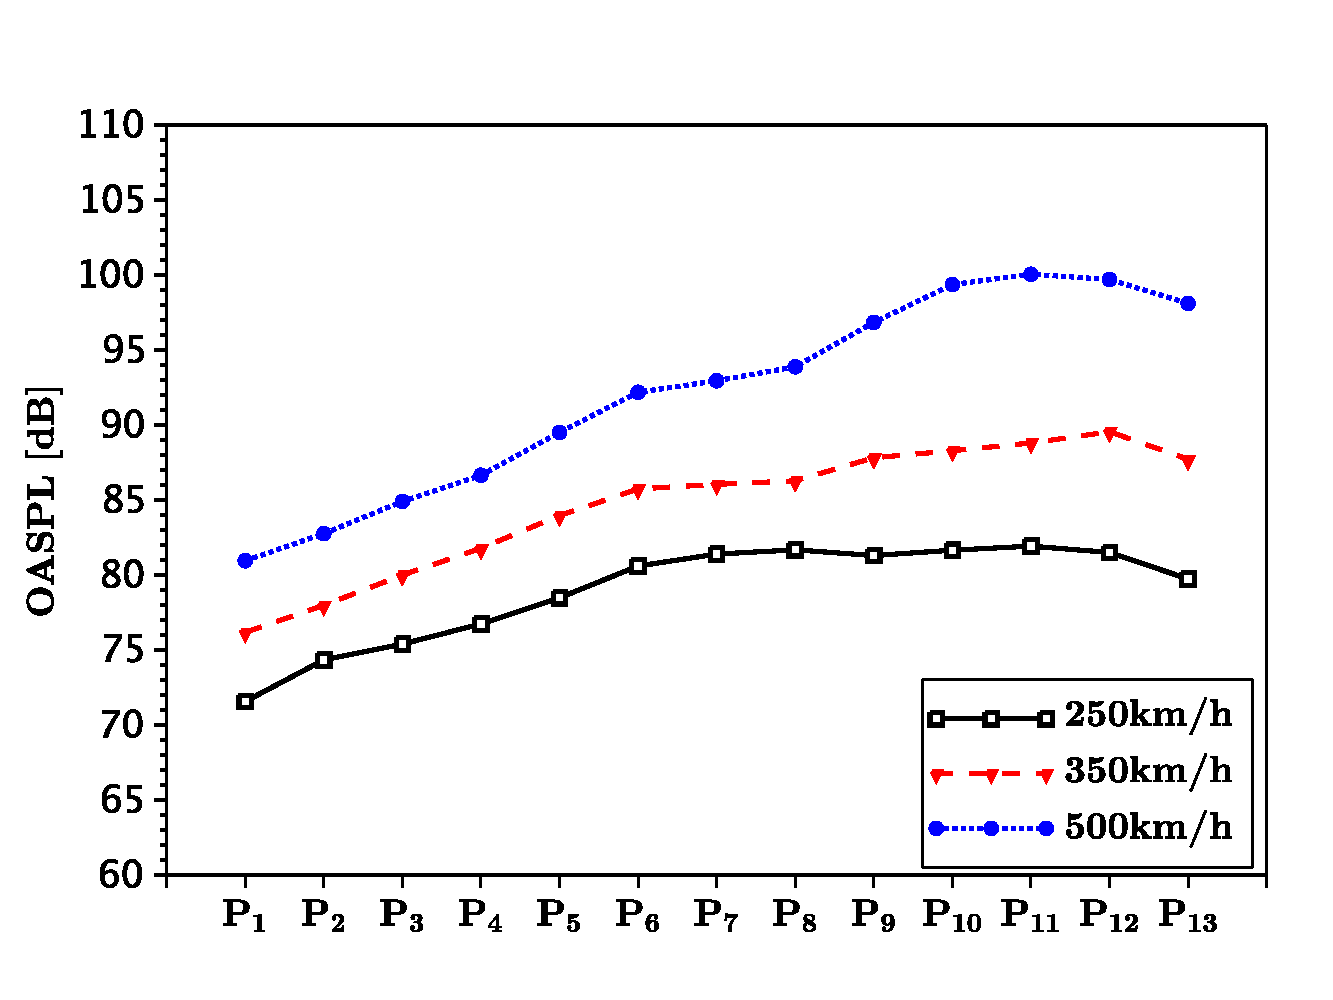
\includegraphics[width=\linewidth]{Figures/oaspl_d.pdf}
    \neusubfigcaption{fig:ch0-four-subfig-d}{工况四}
  \end{neusubfigure}
  \neufigcaption{fig:ch0-four-subfigures}{二乘二子图排版样例}{Example of Two-by-Two Subfigures}
\end{figure}

\neufigref{fig:ch0-four-subfigures} 展示了四幅子图的二乘二排布。
例如 \neusubfigref{fig:ch0-four-subfig-a} 至 \neusubfigref{fig:ch0-four-subfig-d} 可分别引用到四个子图。
排版时建议注意以下几点：
\begin{itemize}
  \item 子图宽度通常可取 \verb|0.48\linewidth| 至 \verb|0.49\linewidth|。
  \item 每行两个子图之间使用 \verb|\hfill| 自动拉开横向间距。
  \item 两行之间可用少量 \verb|\par\vspace| 控制垂直间距。
\end{itemize}

\section{表格排版}

本模板提供 \verb|\neutabcaption{label}{中文题名}{English title}| 用于生成中英文表题。
表题应置于表格上方，正文中使用 \verb|\neutabref{label}| 引用。
表格同样建议使用 \verb|[!htbp]|。如果表格过高导致页底空白，优先考虑缩小字号、调整列宽、拆分表格或使用跨页表格，而不是强制分页。

\subsection{三线表}

\begin{table}[!htbp]
  \centering
  \neutabcaption{tab:ch0-booktabs}{三线表样例}{Example of a Three-Line Table}
  \begin{tabular}{lccc}
    \toprule
    方法       & 准确率（\%）       & 召回率（\%）       & F1 值           \\
    \midrule
    Baseline & 85.2          & 84.1          & 0.846          \\
    Method A & 89.7          & 88.9          & 0.893          \\
    Proposed & \textbf{92.1} & \textbf{91.5} & \textbf{0.918} \\
    \bottomrule
  \end{tabular}
\end{table}

\neutabref{tab:ch0-booktabs} 展示了推荐的三线表格式。
论文中应尽量避免过多竖线，以保持表格简洁。

\subsection{复杂表格}
\begin{table}[!htbp]
  \centering
  \neutabcaption{tab:ch0-complex}{合并单元格与自动换行表格样例}{Example of Merged Cells and Auto-Wrapping Columns}
  \begin{tabularx}{\textwidth}{llXc}
    \toprule
    类别                  & 指标  & 说明                               & 是否必需 \\
    \midrule
    \multirow{2}{*}{图形} & 分辨率 & 位图图片应保证在最终 PDF 中清晰可辨。            & 是    \\
                        & 题名  & 图题使用中英文双语标题，并位于图片下方。             & 是    \\
    \midrule
    \multirow{2}{*}{表格} & 宽度  & 宽表格可使用 \texttt{tabularx} 自动分配列宽。 & 否    \\
                        & 表注  & 表内说明应简明，必要时可在正文中解释。              & 否    \\
    \bottomrule
  \end{tabularx}
\end{table}

\neutabref{tab:ch0-complex} 同时展示了 \verb|\multirow|、\verb|\makecell| 可配合使用的复杂表格场景。
若单元格内容较长，优先使用 \texttt{tabularx} 或 \texttt{p\{...\}} 列类型控制宽度。

\section{公式排版}

公式应使用标准数学环境，并通过 \verb|\label| 设置标签。
引用公式时建议使用模板提供的 \verb|\neueqref{label}|。

\subsection{单行公式}
以分类任务中的交叉熵损失为例，可写为
\begin{equation}
  \mathcal{L}(\theta)
  = - \frac{1}{N}\sum_{i=1}^{N}\sum_{k=1}^{K} y_{ik}\log p_{ik}
  \label{eq:ch0-loss}
\end{equation}

如 \neueqref{eq:ch0-loss} 所示，带编号公式适合放置正文中需要引用的重要定义。

\subsection{多行公式}
循环模型中的状态更新和输出计算可写为
\begin{align}
  h_t       & = \sigma(W_x x_t + W_h h_{t-1} + b), \label{eq:ch0-state} \\
  \hat{y}_t & = \operatorname{softmax}(W_o h_t). \label{eq:ch0-output}
\end{align}

\neueqref{eq:ch0-state} 和 \neueqref{eq:ch0-output} 展示了多行公式的编号方式。
如果多行推导只需要一个编号，可使用 \texttt{aligned} 放在 \texttt{equation} 环境内部。

\subsection{分段函数与矩阵}
分段函数和矩阵经常同时出现在数学定义中，例如
\begin{equation}
  g(x)=
  \begin{cases}
    0, & x < 0,       \\
    x, & 0 \le x < 1, \\
    1, & x \ge 1,
  \end{cases}
  \qquad
  A =
  \begin{bmatrix}
    1 & 0 & 0 \\
    0 & 1 & 0 \\
    0 & 0 & 1
  \end{bmatrix}.
  \label{eq:ch0-piecewise}
\end{equation}

\neueqref{eq:ch0-piecewise} 展示了分段函数和矩阵的常见写法。

\section{算法伪代码}

计算机类论文常需要给出算法步骤。本文档在 \texttt{main.tex} 中加载了 \texttt{algorithm} 和 \texttt{algorithmic} 宏包，可以直接使用如下环境。

\begin{algorithm}[!htbp]
  \caption{样例训练流程}
  \label{alg:ch0-training}
  \begin{algorithmic}[1]
    \REQUIRE Training set $\mathcal{D}$, learning rate $\eta$, maximum epoch $T$
    \ENSURE Model parameters $\theta$
    \STATE Initialize parameters $\theta$
    \FOR{$t = 1$ to $T$}
    \STATE Sample a mini-batch $\mathcal{B}$ from $\mathcal{D}$
    \STATE Compute loss $\mathcal{L}(\theta)$ by \neueqref{eq:ch0-loss}
    \STATE Update $\theta \leftarrow \theta - \eta \nabla_{\theta}\mathcal{L}(\theta)$
    \ENDFOR
    \RETURN $\theta$
  \end{algorithmic}
\end{algorithm}

算法~\ref{alg:ch0-training} 展示了带行号的伪代码。
若需要中文关键字，可在导言区重定义相应命令。

\section{引用、链接与交叉引用}

参考文献引用可使用两种模板命令：
\begin{itemize}
  \item 上标引用使用 \verb|\upcite{key}|，适合放在句末，例如已有研究讨论了神经网络轻量化问题\upcite{guo_2023_research}。
  \item 正文引用使用 \verb|\inlinecite{key}|，适合作为句子成分，例如文献 \inlinecite{thakkar_2018_performance} 给出了系统性能评测案例。
\end{itemize}
多篇文献可写在同一条引用命令中，例如区块链平台相关研究\upcite{zheng_2019_nutbaas,thakkar_2018_performance}。

交叉引用建议统一使用模板命令：
\begin{itemize}
  \item 图引用：\verb|\neufigref{fig:ch0-pdf}|，效果为 \neufigref{fig:ch0-pdf}。
  \item 子图引用：\verb|\neusubfigref{fig:ch0-four-subfig-a}|，效果为 \neusubfigref{fig:ch0-four-subfig-a}。
  \item 表引用：\verb|\neutabref{tab:ch0-complex}|，效果为 \neutabref{tab:ch0-complex}。
  \item 公式引用：\verb|\neueqref{eq:ch0-loss}|，效果为 \neueqref{eq:ch0-loss}。
  \item 算法引用：当前模板未单独封装算法引用命令，可写作“算法~\ref{alg:ch0-training}”。
\end{itemize}
模板提供的公开命令和环境可参考 \texttt{README.md} 中的“模板命令说明”一节。
|，并从第~\ref{chap:introduction}~章开始组织正式内容。

\section{章节层级与正文段落}

论文正文通常从一级标题开始组织内容，一级标题使用 \verb|\chapter|，二级标题使用 \verb|\section|，三级标题使用 \verb|\subsection|。
本模板会自动设置章标题、节标题、页眉、页码和目录格式，作者只需要关注正文内容。
正文段落首行缩进、行距和中英文字体均由模板统一控制，一般不需要在正文中手动设置字号、字体或段间距。

中文正文可以直接书写；英文术语建议在首次出现时给出全称，例如自然语言处理（Natural Language Processing, NLP）。
行内公式可以写作 $E=mc^2$，行内代码或命令可以使用 \verb|\verb|，例如 \verb|%!TEX root = ./main.tex
\chapter{论文格式样例与模板验证}

本章作为模板的集中样例章，用于快速检查正文中常见排版元素的显示效果。
样例覆盖章节层级、正文段落、列表、脚注、图、表、公式、算法、交叉引用和参考文献引用等内容。
编写正式论文时，可以保留本章作为排版对照；定稿前可在 \texttt{main.tex} 中删除或注释 \verb|\input{chapter0-guide}|，并从第~\ref{chap:introduction}~章开始组织正式内容。

\section{章节层级与正文段落}

论文正文通常从一级标题开始组织内容，一级标题使用 \verb|\chapter|，二级标题使用 \verb|\section|，三级标题使用 \verb|\subsection|。
本模板会自动设置章标题、节标题、页眉、页码和目录格式，作者只需要关注正文内容。
正文段落首行缩进、行距和中英文字体均由模板统一控制，一般不需要在正文中手动设置字号、字体或段间距。

中文正文可以直接书写；英文术语建议在首次出现时给出全称，例如自然语言处理（Natural Language Processing, NLP）。
行内公式可以写作 $E=mc^2$，行内代码或命令可以使用 \verb|\verb|，例如 \verb|\input{chapter0-guide}|。
脚注示例如此处所示\footnote{脚注用于补充说明，不宜放置过长的正文内容。}。
若某页因图表浮动或分页规则没有排满，脚注可能跟随正文排版区而显得略高，这是正常的 LaTeX 页面构建结果。

\subsection{字体、字号与强调}

模板预定义了常用中文字体命令。正式论文中通常不需要手动切换字体；只有在展示样式、术语强调或特殊说明时才建议使用。
当前模板已经为默认宋体和 \verb|\song| 字族配置伪粗体，因此 \verb|\textbf| 或 \verb|\bfseries| 可以用于中文局部强调。
需要注意的是，中文加粗应克制使用；标题层级、术语定义或表格重点值可以适当加粗，大段正文不建议整体加粗。
如果需要更明显的标题式强调，可使用黑体或调整标题层级；如果只是普通正文重点，优先使用 \verb|\textbf|。

\begin{table}[!htbp]
  \centering
  \neutabcaption{tab:ch0-fonts}{字体与强调样例}{Examples of Fonts and Emphasis}
  \begin{tabular}{lll}
    \toprule
    命令             & 显示效果                         & 使用建议       \\
    \midrule
    \verb|\song|   & {\song 宋体文字示例}               & 正文默认字体     \\
    \verb|\textbf| & \textbf{加粗文字示例}              & 局部强调、表格重点值 \\
    \verb|\hei|    & {\hei 黑体文字示例}                & 标题或较强强调场景  \\
    \verb|\kai|    & {\kai 楷体文字示例}                & 摘要、题签或引用语  \\
    \verb|\fs|     & {\fs 仿宋文字示例}                 & 特殊文书类内容    \\
    \verb|\textit| & \textit{Italic text example} & 英文斜体或变量说明  \\
    \bottomrule
  \end{tabular}
\end{table}

\subsection{列表环境}

无序列表适合列出并列事项：
\begin{itemize}
  \item 图题位于图下方，表题位于表上方。
  \item 图表应使用中英文双语标题。
  \item 公式、图、表、算法均应使用标签进行交叉引用。
\end{itemize}

有序列表适合描述步骤：
\begin{enumerate}
  \item 在 \texttt{main.tex} 中填写论文元信息。
  \item 在各章文件中撰写正文内容。
  \item 使用 \texttt{latexmk -xelatex main.tex} 完成编译。
\end{enumerate}

\section{图形排版}

本模板提供 \verb|\neufigcaption{label}{中文题名}{English title}| 用于生成中英文图题。
图题应置于图形下方，正文中使用 \verb|\neufigref{label}| 引用。
图形建议使用 \verb|[!htbp]| 浮动参数，让 LaTeX 在当前位置、页顶、页底或浮动页中选择较合适的位置；除非必须固定位置，否则不建议使用 \verb|[H]|。

\subsection{外部图片}
\begin{figure}[!htbp]
  \centering
  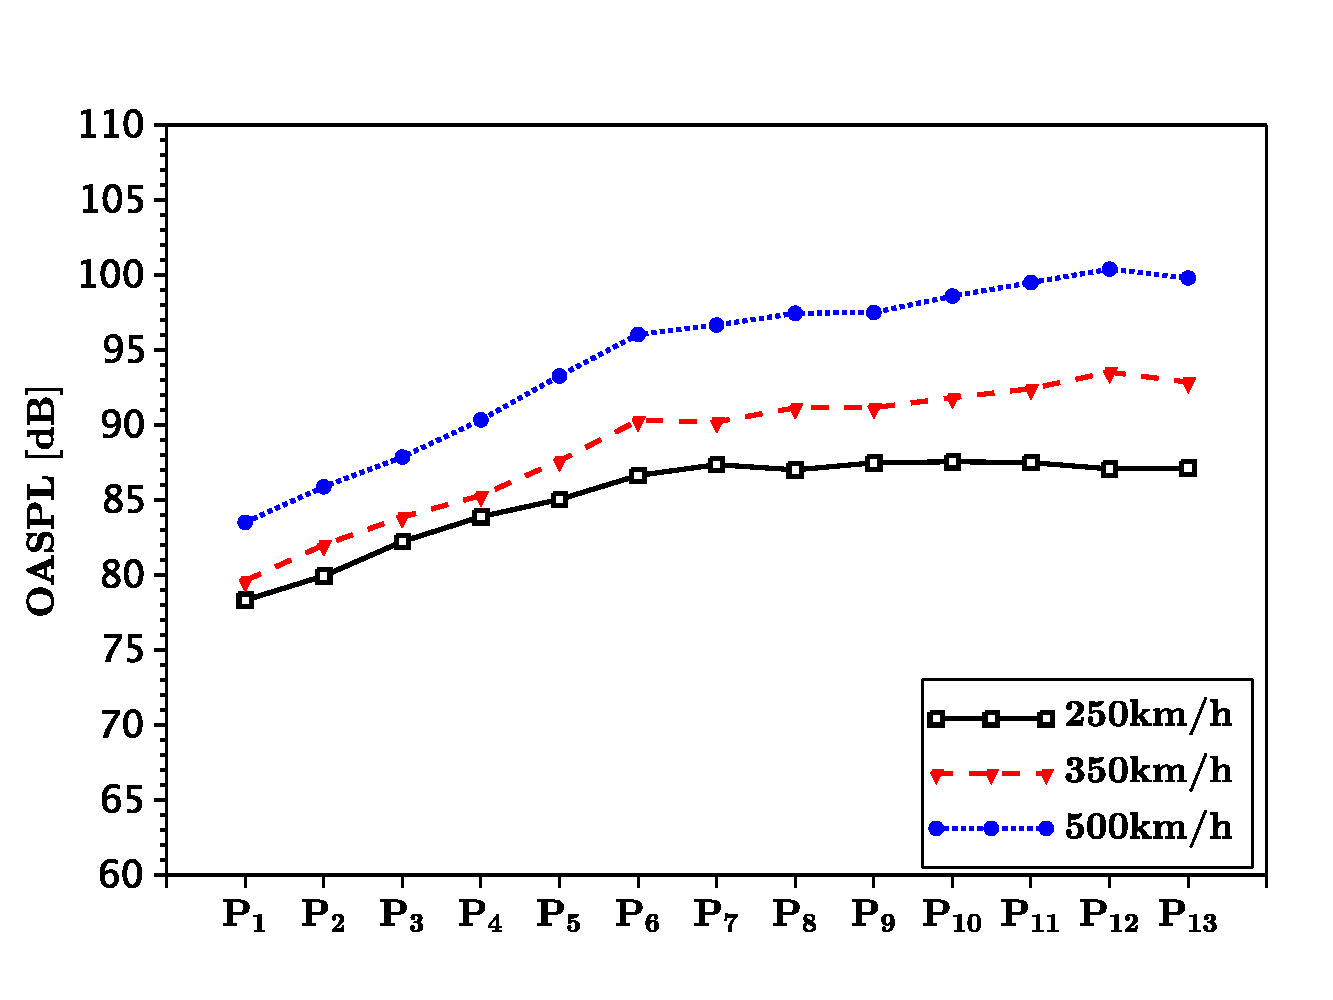
\includegraphics[width=0.55\textwidth]{Figures/oaspl_a.pdf}
  \neufigcaption{fig:ch0-cover}{外部图片插入样例}{Example of Including an External Image}
\end{figure}

\neufigref{fig:ch0-cover} 展示了通过 \verb|\includegraphics| 插入图片文件的方式。
正式论文中建议将图片统一放入 \texttt{Figures} 目录，并使用相对路径引用。

\subsection{PDF 或位图图片}
\begin{figure}[!htbp]
  \centering
  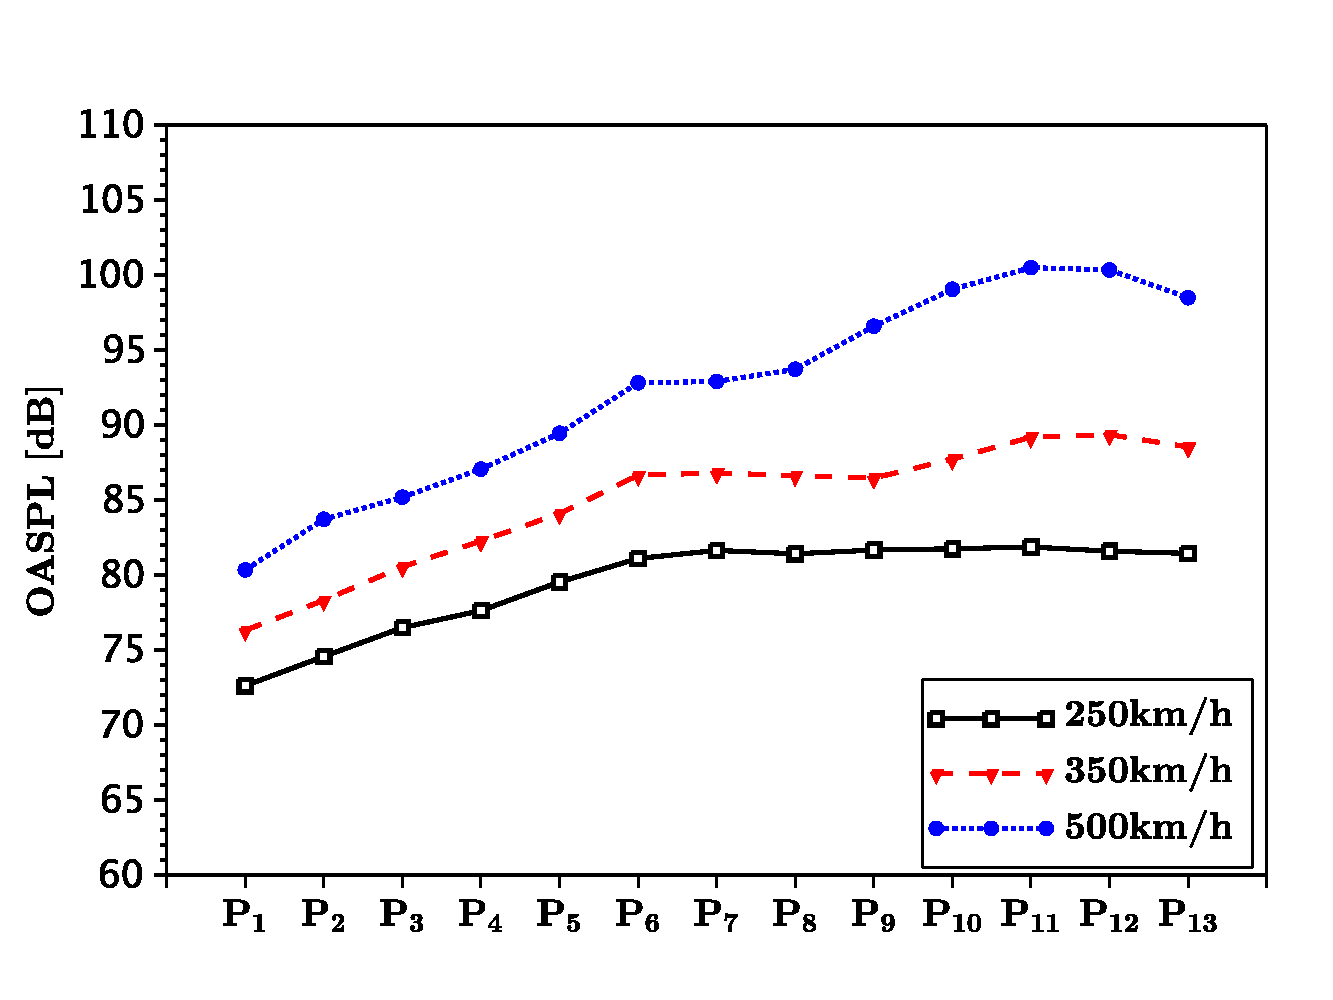
\includegraphics[width=0.55\textwidth]{Figures/oaspl_b.pdf}
  \neufigcaption{fig:ch0-pdf}{PDF 图片插入样例}{Example of Including a PDF Figure}
\end{figure}

PDF、PNG、JPG 等常见图片格式均可通过 \verb|\includegraphics| 插入。
若图片由绘图软件或数据分析程序导出，建议优先使用 PDF 格式以保持较清晰的显示效果。

\subsection{并列图片}
\begin{figure}[!htbp]
  \centering
  \begin{minipage}[t]{0.49\linewidth}
    \centering
    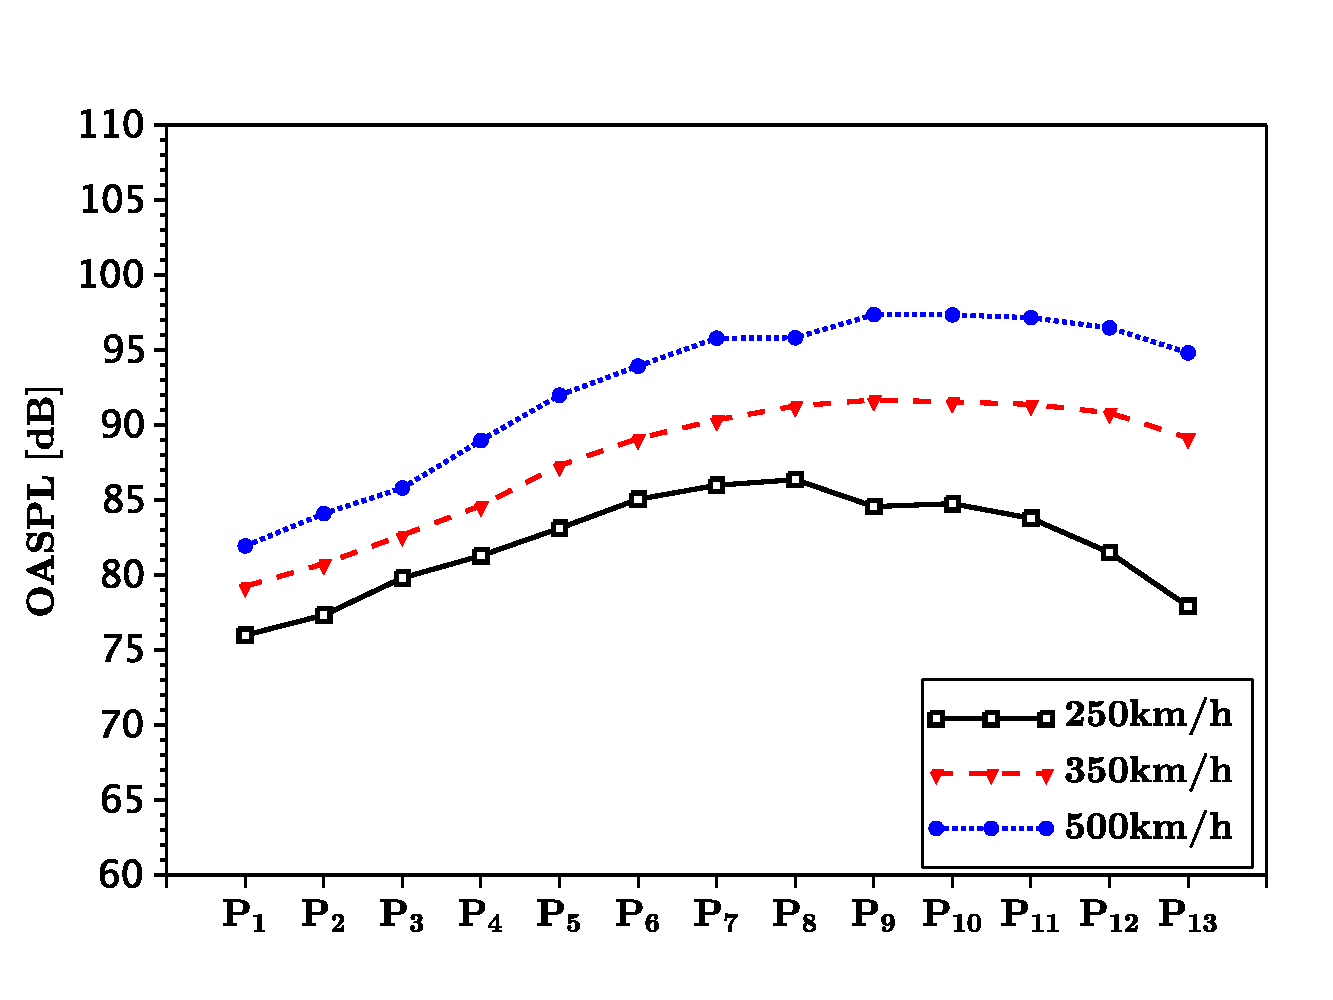
\includegraphics[width=\linewidth]{Figures/oaspl_c.pdf}
  \end{minipage}
  \hfill
  \begin{minipage}[t]{0.49\linewidth}
    \centering
    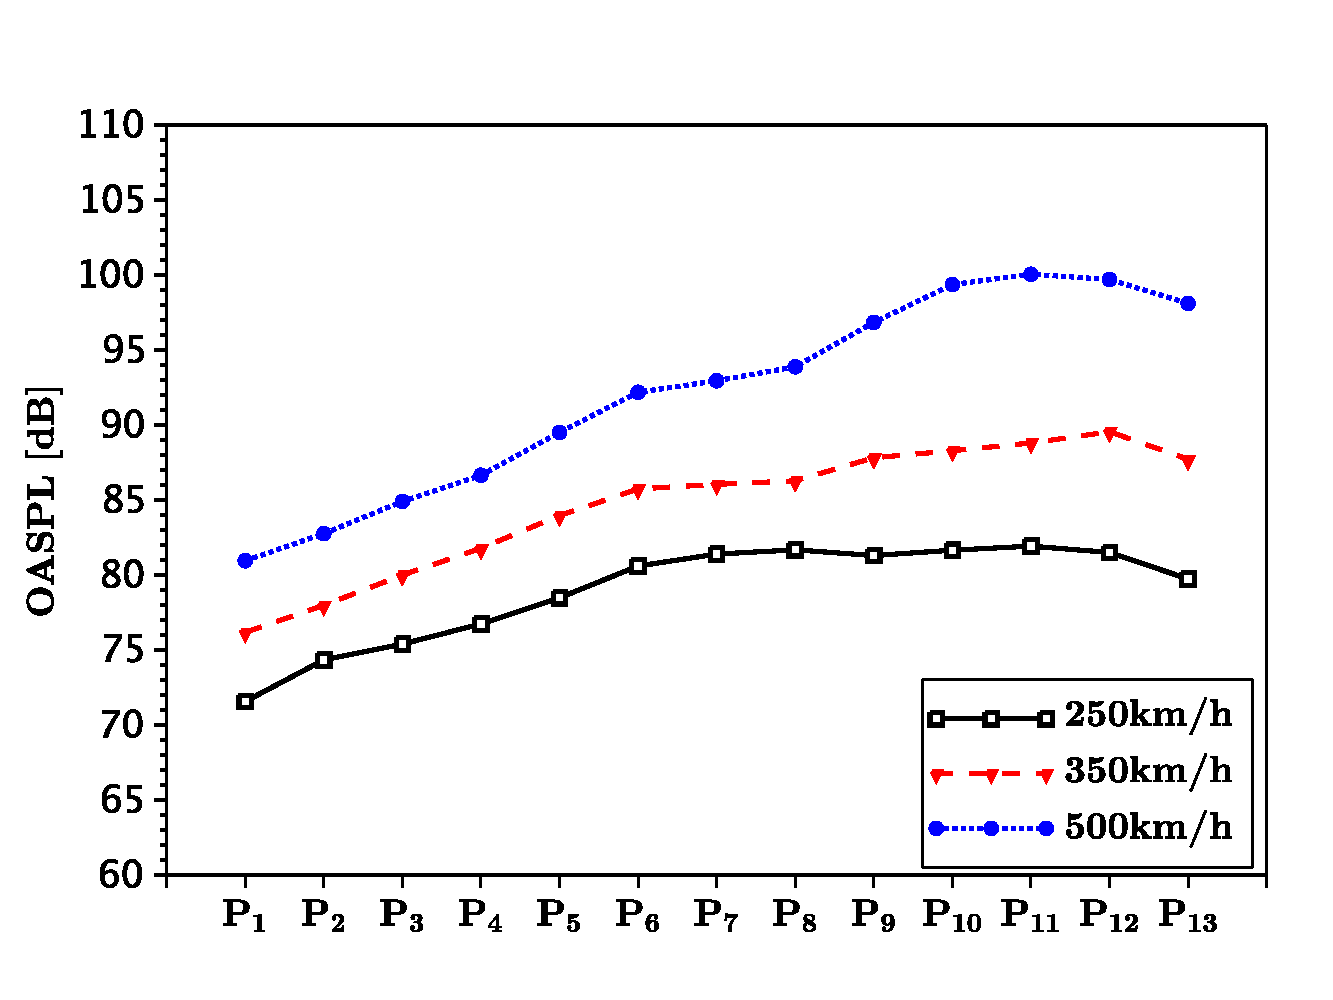
\includegraphics[width=\linewidth]{Figures/oaspl_d.pdf}
  \end{minipage}
  \neufigcaption{fig:ch0-side-by-side}{普通并列图形排版样例}{Example of Side-by-Side Figures}
\end{figure}

\neufigref{fig:ch0-side-by-side} 使用 \texttt{minipage} 完成普通并列排版。
当两幅图共享一个总标题且不需要分别引用时，可使用这种方式。

\subsection{并列子图}
\begin{figure}[!htbp]
  \centering
  \begin{neusubfigure}{0.49\linewidth}
    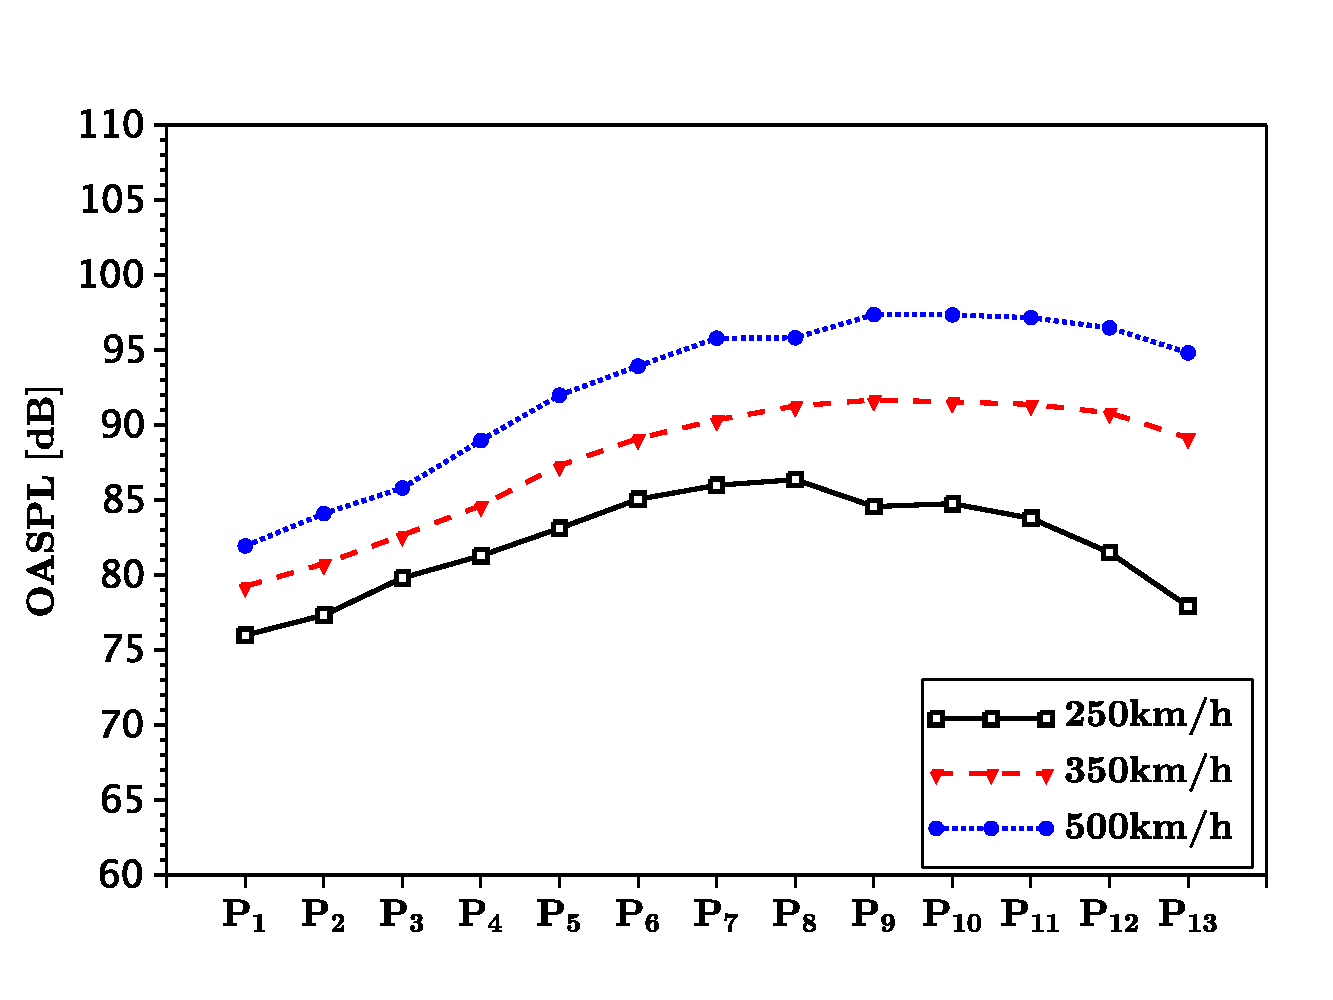
\includegraphics[width=\linewidth]{Figures/oaspl_c.pdf}
    \neusubfigcaption{fig:ch0-side-by-side-a}{工况一}
  \end{neusubfigure}
  \hfill
  \begin{neusubfigure}{0.49\linewidth}
    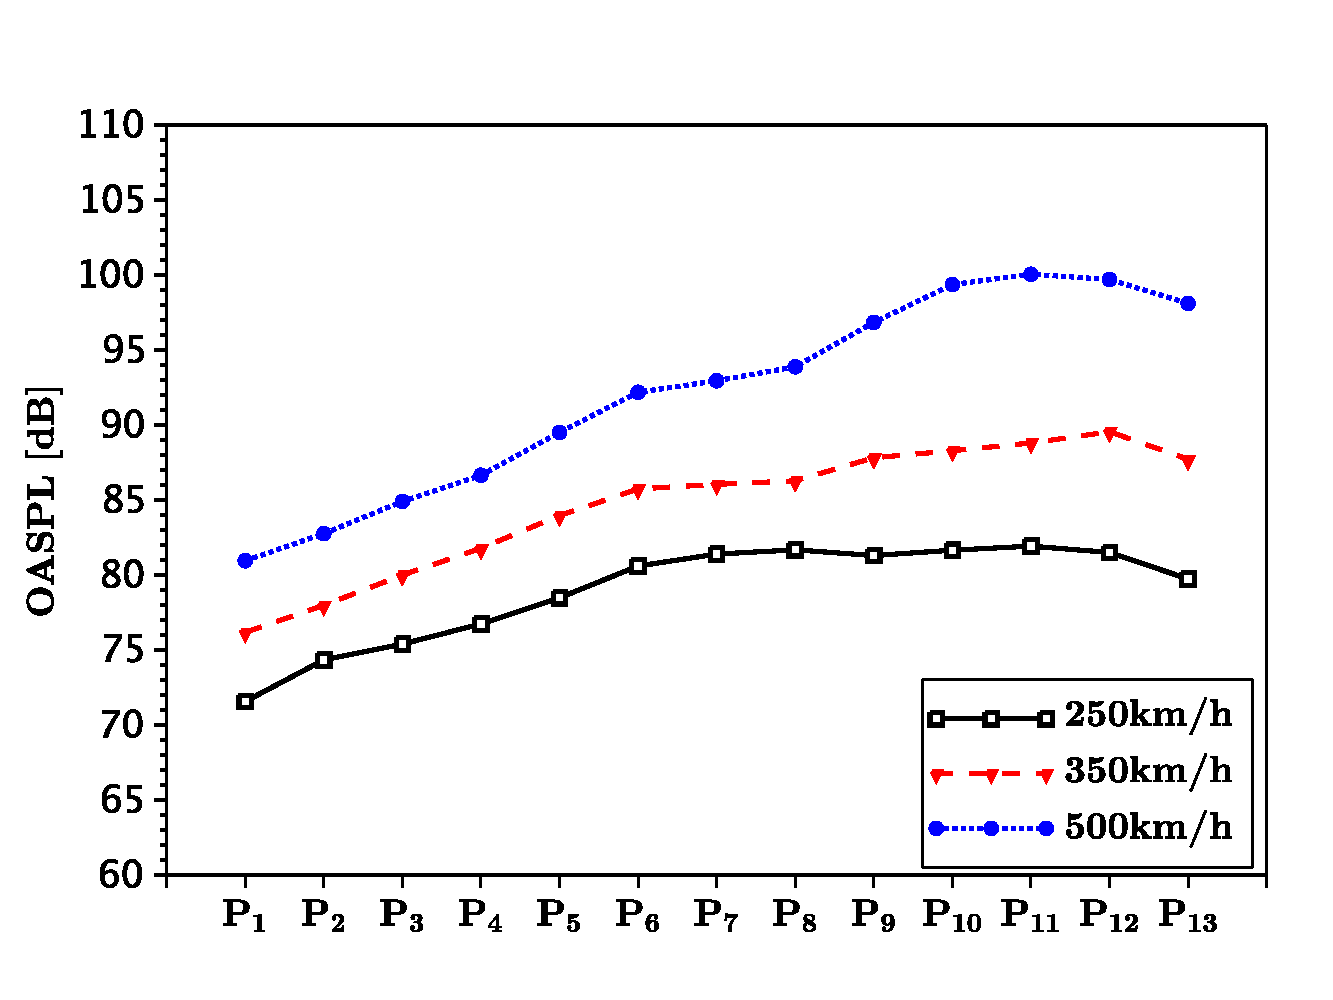
\includegraphics[width=\linewidth]{Figures/oaspl_d.pdf}
    \neusubfigcaption{fig:ch0-side-by-side-b}{工况二}
  \end{neusubfigure}
  \neufigcaption{fig:ch0-subfigures}{并列子图排版样例}{Example of Side-by-Side Subfigures}
\end{figure}

\neufigref{fig:ch0-subfigures} 使用 \texttt{neusubfigure} 完成并列子图排版。
其中 \neusubfigref{fig:ch0-side-by-side-a} 和 \neusubfigref{fig:ch0-side-by-side-b} 可分别引用到子图。
当两幅图共享一个总标题且需要分别引用时，可使用这种方式；如果每幅图需要完全独立的图号，建议拆成两个独立的 \texttt{figure} 环境。

\subsection{二乘二子图}
\begin{figure}[!htbp]
  \centering
  \begin{neusubfigure}{0.49\linewidth}
    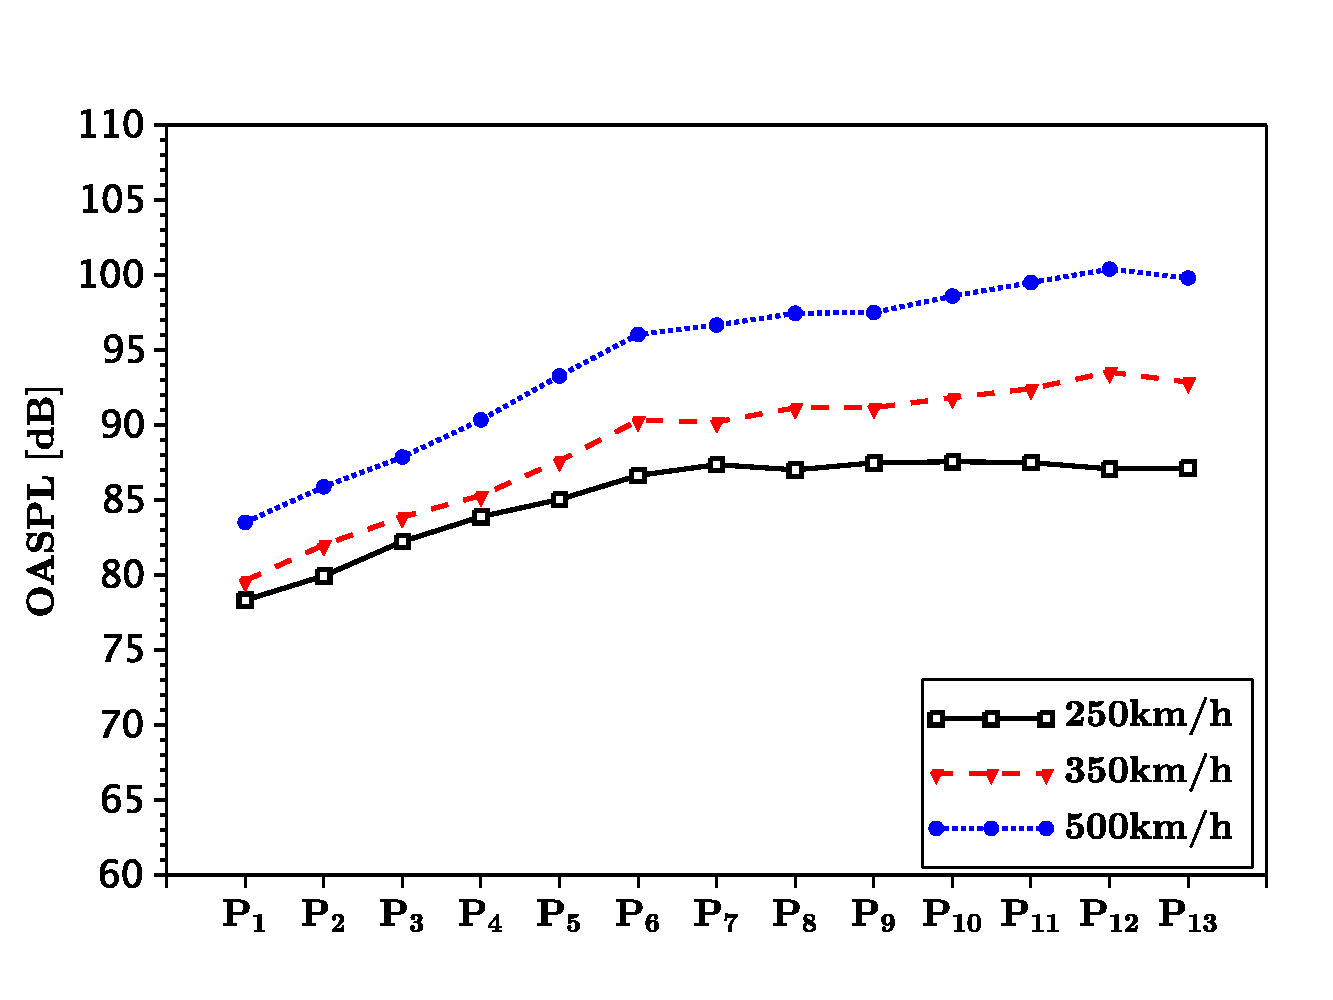
\includegraphics[width=\linewidth]{Figures/oaspl_a.pdf}
    \neusubfigcaption{fig:ch0-four-subfig-a}{工况一}
  \end{neusubfigure}
  \hfill
  \begin{neusubfigure}{0.49\linewidth}
    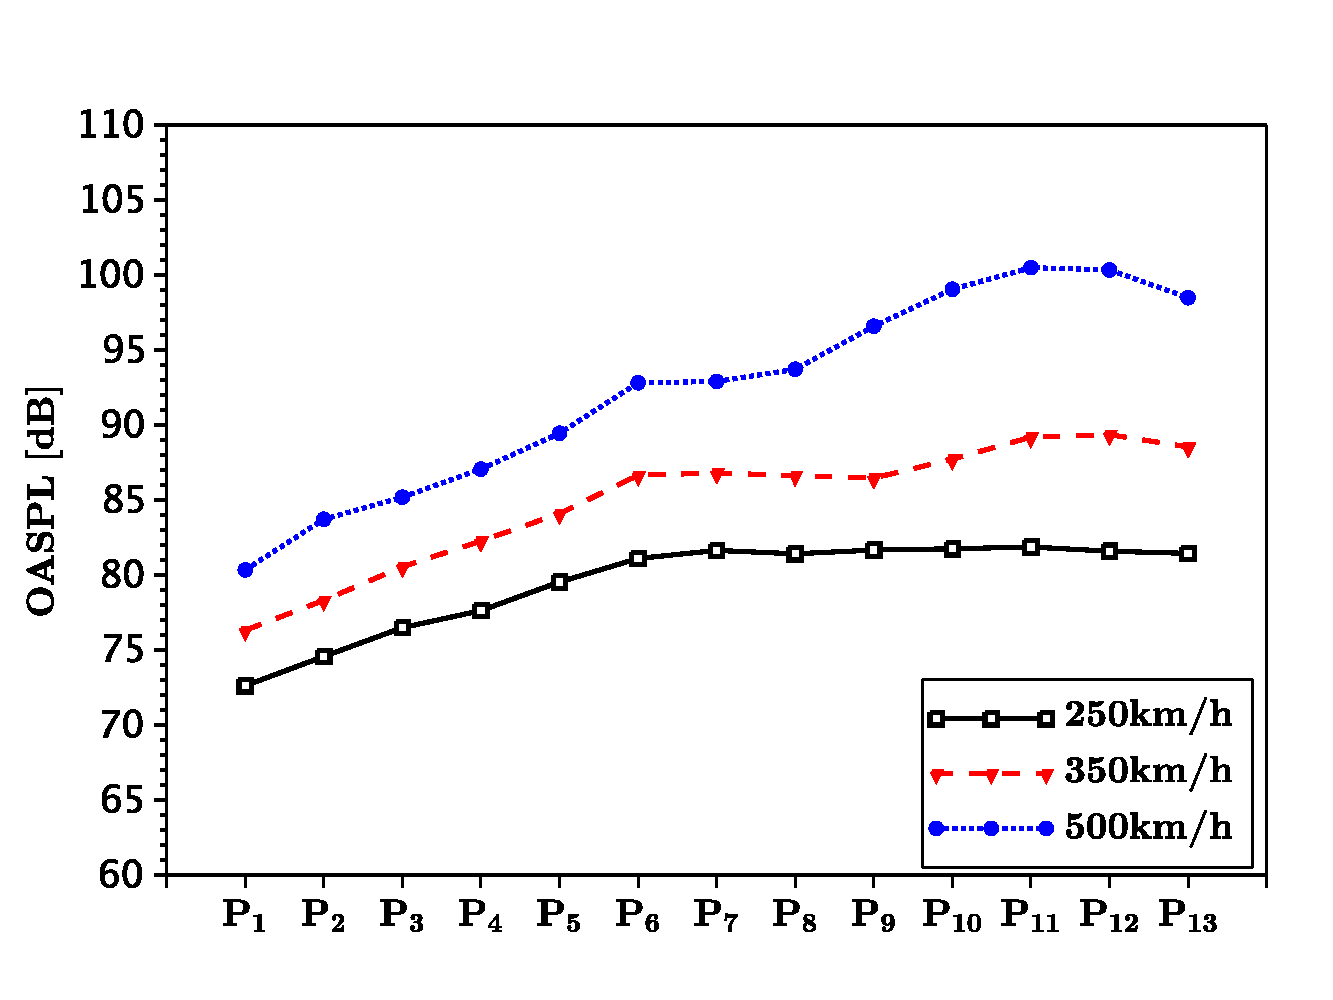
\includegraphics[width=\linewidth]{Figures/oaspl_b.pdf}
    \neusubfigcaption{fig:ch0-four-subfig-b}{工况二}
  \end{neusubfigure}
  \par\vspace{2bp}

  \begin{neusubfigure}{0.49\linewidth}
    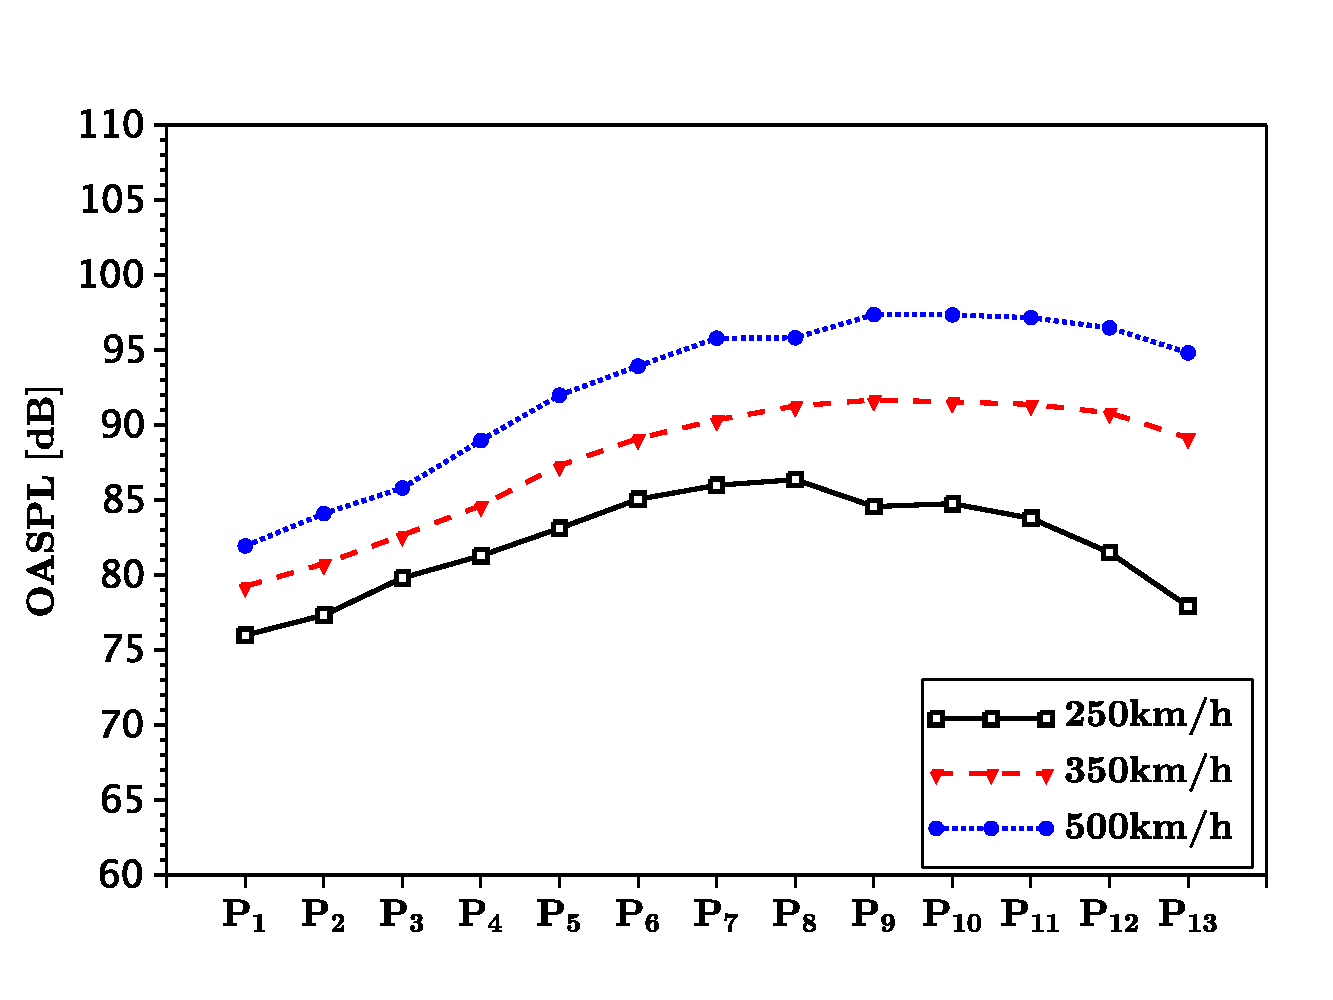
\includegraphics[width=\linewidth]{Figures/oaspl_c.pdf}
    \neusubfigcaption{fig:ch0-four-subfig-c}{工况三}
  \end{neusubfigure}
  \hfill
  \begin{neusubfigure}{0.49\linewidth}
    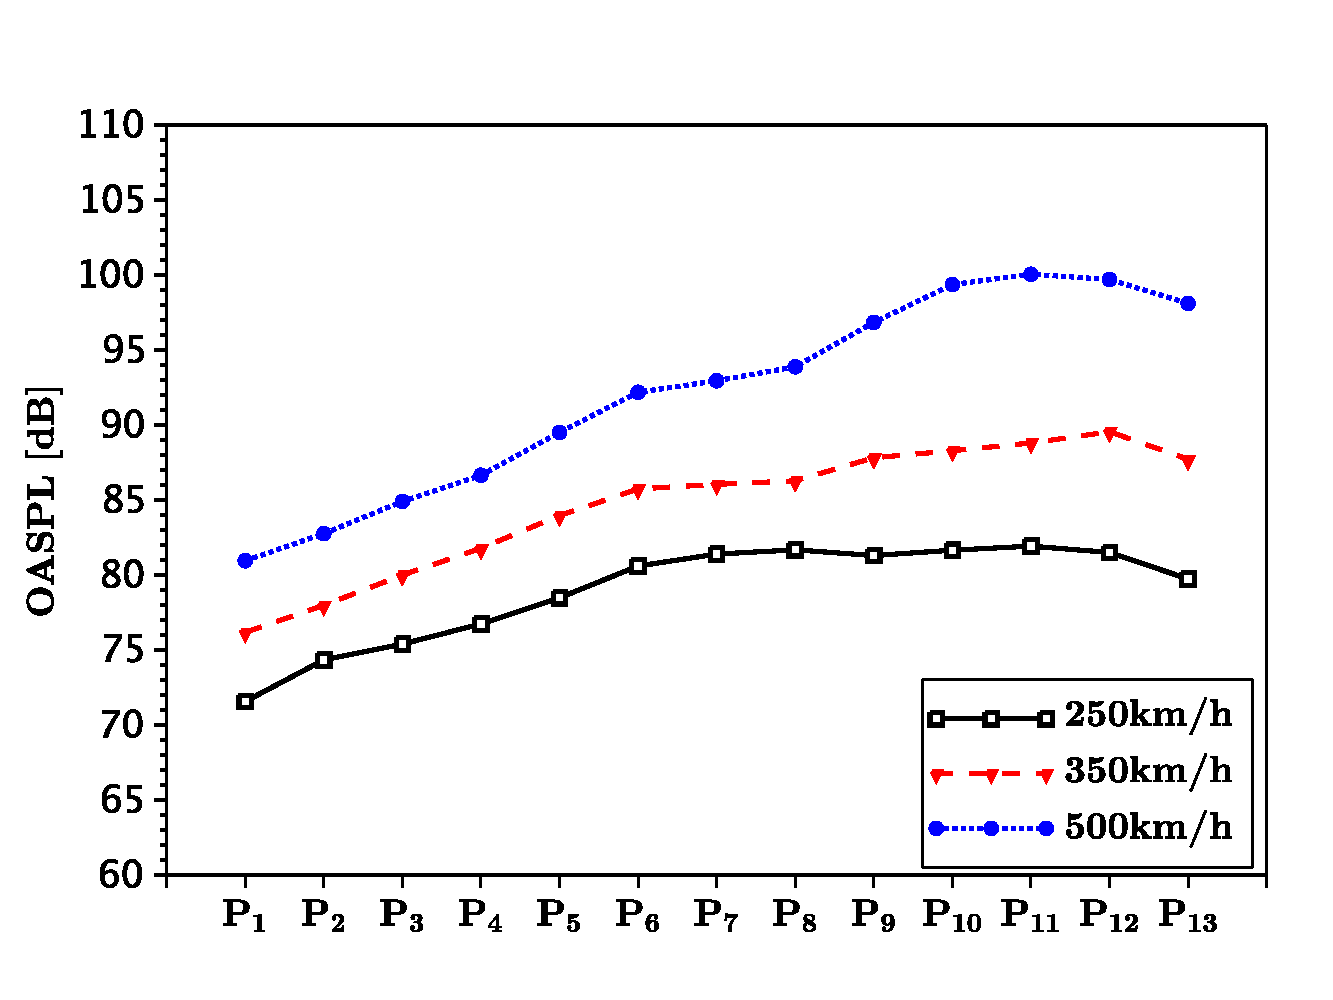
\includegraphics[width=\linewidth]{Figures/oaspl_d.pdf}
    \neusubfigcaption{fig:ch0-four-subfig-d}{工况四}
  \end{neusubfigure}
  \neufigcaption{fig:ch0-four-subfigures}{二乘二子图排版样例}{Example of Two-by-Two Subfigures}
\end{figure}

\neufigref{fig:ch0-four-subfigures} 展示了四幅子图的二乘二排布。
例如 \neusubfigref{fig:ch0-four-subfig-a} 至 \neusubfigref{fig:ch0-four-subfig-d} 可分别引用到四个子图。
排版时建议注意以下几点：
\begin{itemize}
  \item 子图宽度通常可取 \verb|0.48\linewidth| 至 \verb|0.49\linewidth|。
  \item 每行两个子图之间使用 \verb|\hfill| 自动拉开横向间距。
  \item 两行之间可用少量 \verb|\par\vspace| 控制垂直间距。
\end{itemize}

\section{表格排版}

本模板提供 \verb|\neutabcaption{label}{中文题名}{English title}| 用于生成中英文表题。
表题应置于表格上方，正文中使用 \verb|\neutabref{label}| 引用。
表格同样建议使用 \verb|[!htbp]|。如果表格过高导致页底空白，优先考虑缩小字号、调整列宽、拆分表格或使用跨页表格，而不是强制分页。

\subsection{三线表}

\begin{table}[!htbp]
  \centering
  \neutabcaption{tab:ch0-booktabs}{三线表样例}{Example of a Three-Line Table}
  \begin{tabular}{lccc}
    \toprule
    方法       & 准确率（\%）       & 召回率（\%）       & F1 值           \\
    \midrule
    Baseline & 85.2          & 84.1          & 0.846          \\
    Method A & 89.7          & 88.9          & 0.893          \\
    Proposed & \textbf{92.1} & \textbf{91.5} & \textbf{0.918} \\
    \bottomrule
  \end{tabular}
\end{table}

\neutabref{tab:ch0-booktabs} 展示了推荐的三线表格式。
论文中应尽量避免过多竖线，以保持表格简洁。

\subsection{复杂表格}
\begin{table}[!htbp]
  \centering
  \neutabcaption{tab:ch0-complex}{合并单元格与自动换行表格样例}{Example of Merged Cells and Auto-Wrapping Columns}
  \begin{tabularx}{\textwidth}{llXc}
    \toprule
    类别                  & 指标  & 说明                               & 是否必需 \\
    \midrule
    \multirow{2}{*}{图形} & 分辨率 & 位图图片应保证在最终 PDF 中清晰可辨。            & 是    \\
                        & 题名  & 图题使用中英文双语标题，并位于图片下方。             & 是    \\
    \midrule
    \multirow{2}{*}{表格} & 宽度  & 宽表格可使用 \texttt{tabularx} 自动分配列宽。 & 否    \\
                        & 表注  & 表内说明应简明，必要时可在正文中解释。              & 否    \\
    \bottomrule
  \end{tabularx}
\end{table}

\neutabref{tab:ch0-complex} 同时展示了 \verb|\multirow|、\verb|\makecell| 可配合使用的复杂表格场景。
若单元格内容较长，优先使用 \texttt{tabularx} 或 \texttt{p\{...\}} 列类型控制宽度。

\section{公式排版}

公式应使用标准数学环境，并通过 \verb|\label| 设置标签。
引用公式时建议使用模板提供的 \verb|\neueqref{label}|。

\subsection{单行公式}
以分类任务中的交叉熵损失为例，可写为
\begin{equation}
  \mathcal{L}(\theta)
  = - \frac{1}{N}\sum_{i=1}^{N}\sum_{k=1}^{K} y_{ik}\log p_{ik}
  \label{eq:ch0-loss}
\end{equation}

如 \neueqref{eq:ch0-loss} 所示，带编号公式适合放置正文中需要引用的重要定义。

\subsection{多行公式}
循环模型中的状态更新和输出计算可写为
\begin{align}
  h_t       & = \sigma(W_x x_t + W_h h_{t-1} + b), \label{eq:ch0-state} \\
  \hat{y}_t & = \operatorname{softmax}(W_o h_t). \label{eq:ch0-output}
\end{align}

\neueqref{eq:ch0-state} 和 \neueqref{eq:ch0-output} 展示了多行公式的编号方式。
如果多行推导只需要一个编号，可使用 \texttt{aligned} 放在 \texttt{equation} 环境内部。

\subsection{分段函数与矩阵}
分段函数和矩阵经常同时出现在数学定义中，例如
\begin{equation}
  g(x)=
  \begin{cases}
    0, & x < 0,       \\
    x, & 0 \le x < 1, \\
    1, & x \ge 1,
  \end{cases}
  \qquad
  A =
  \begin{bmatrix}
    1 & 0 & 0 \\
    0 & 1 & 0 \\
    0 & 0 & 1
  \end{bmatrix}.
  \label{eq:ch0-piecewise}
\end{equation}

\neueqref{eq:ch0-piecewise} 展示了分段函数和矩阵的常见写法。

\section{算法伪代码}

计算机类论文常需要给出算法步骤。本文档在 \texttt{main.tex} 中加载了 \texttt{algorithm} 和 \texttt{algorithmic} 宏包，可以直接使用如下环境。

\begin{algorithm}[!htbp]
  \caption{样例训练流程}
  \label{alg:ch0-training}
  \begin{algorithmic}[1]
    \REQUIRE Training set $\mathcal{D}$, learning rate $\eta$, maximum epoch $T$
    \ENSURE Model parameters $\theta$
    \STATE Initialize parameters $\theta$
    \FOR{$t = 1$ to $T$}
    \STATE Sample a mini-batch $\mathcal{B}$ from $\mathcal{D}$
    \STATE Compute loss $\mathcal{L}(\theta)$ by \neueqref{eq:ch0-loss}
    \STATE Update $\theta \leftarrow \theta - \eta \nabla_{\theta}\mathcal{L}(\theta)$
    \ENDFOR
    \RETURN $\theta$
  \end{algorithmic}
\end{algorithm}

算法~\ref{alg:ch0-training} 展示了带行号的伪代码。
若需要中文关键字，可在导言区重定义相应命令。

\section{引用、链接与交叉引用}

参考文献引用可使用两种模板命令：
\begin{itemize}
  \item 上标引用使用 \verb|\upcite{key}|，适合放在句末，例如已有研究讨论了神经网络轻量化问题\upcite{guo_2023_research}。
  \item 正文引用使用 \verb|\inlinecite{key}|，适合作为句子成分，例如文献 \inlinecite{thakkar_2018_performance} 给出了系统性能评测案例。
\end{itemize}
多篇文献可写在同一条引用命令中，例如区块链平台相关研究\upcite{zheng_2019_nutbaas,thakkar_2018_performance}。

交叉引用建议统一使用模板命令：
\begin{itemize}
  \item 图引用：\verb|\neufigref{fig:ch0-pdf}|，效果为 \neufigref{fig:ch0-pdf}。
  \item 子图引用：\verb|\neusubfigref{fig:ch0-four-subfig-a}|，效果为 \neusubfigref{fig:ch0-four-subfig-a}。
  \item 表引用：\verb|\neutabref{tab:ch0-complex}|，效果为 \neutabref{tab:ch0-complex}。
  \item 公式引用：\verb|\neueqref{eq:ch0-loss}|，效果为 \neueqref{eq:ch0-loss}。
  \item 算法引用：当前模板未单独封装算法引用命令，可写作“算法~\ref{alg:ch0-training}”。
\end{itemize}
模板提供的公开命令和环境可参考 \texttt{README.md} 中的“模板命令说明”一节。
|。
脚注示例如此处所示\footnote{脚注用于补充说明，不宜放置过长的正文内容。}。
若某页因图表浮动或分页规则没有排满，脚注可能跟随正文排版区而显得略高，这是正常的 LaTeX 页面构建结果。

\subsection{字体、字号与强调}

模板预定义了常用中文字体命令。正式论文中通常不需要手动切换字体；只有在展示样式、术语强调或特殊说明时才建议使用。
当前模板已经为默认宋体和 \verb|\song| 字族配置伪粗体，因此 \verb|\textbf| 或 \verb|\bfseries| 可以用于中文局部强调。
需要注意的是，中文加粗应克制使用；标题层级、术语定义或表格重点值可以适当加粗，大段正文不建议整体加粗。
如果需要更明显的标题式强调，可使用黑体或调整标题层级；如果只是普通正文重点，优先使用 \verb|\textbf|。

\begin{table}[!htbp]
  \centering
  \neutabcaption{tab:ch0-fonts}{字体与强调样例}{Examples of Fonts and Emphasis}
  \begin{tabular}{lll}
    \toprule
    命令             & 显示效果                         & 使用建议       \\
    \midrule
    \verb|\song|   & {\song 宋体文字示例}               & 正文默认字体     \\
    \verb|\textbf| & \textbf{加粗文字示例}              & 局部强调、表格重点值 \\
    \verb|\hei|    & {\hei 黑体文字示例}                & 标题或较强强调场景  \\
    \verb|\kai|    & {\kai 楷体文字示例}                & 摘要、题签或引用语  \\
    \verb|\fs|     & {\fs 仿宋文字示例}                 & 特殊文书类内容    \\
    \verb|\textit| & \textit{Italic text example} & 英文斜体或变量说明  \\
    \bottomrule
  \end{tabular}
\end{table}

\subsection{列表环境}

无序列表适合列出并列事项：
\begin{itemize}
  \item 图题位于图下方，表题位于表上方。
  \item 图表应使用中英文双语标题。
  \item 公式、图、表、算法均应使用标签进行交叉引用。
\end{itemize}

有序列表适合描述步骤：
\begin{enumerate}
  \item 在 \texttt{main.tex} 中填写论文元信息。
  \item 在各章文件中撰写正文内容。
  \item 使用 \texttt{latexmk -xelatex main.tex} 完成编译。
\end{enumerate}

\section{图形排版}

本模板提供 \verb|\neufigcaption{label}{中文题名}{English title}| 用于生成中英文图题。
图题应置于图形下方，正文中使用 \verb|\neufigref{label}| 引用。
图形建议使用 \verb|[!htbp]| 浮动参数，让 LaTeX 在当前位置、页顶、页底或浮动页中选择较合适的位置；除非必须固定位置，否则不建议使用 \verb|[H]|。

\subsection{外部图片}
\begin{figure}[!htbp]
  \centering
  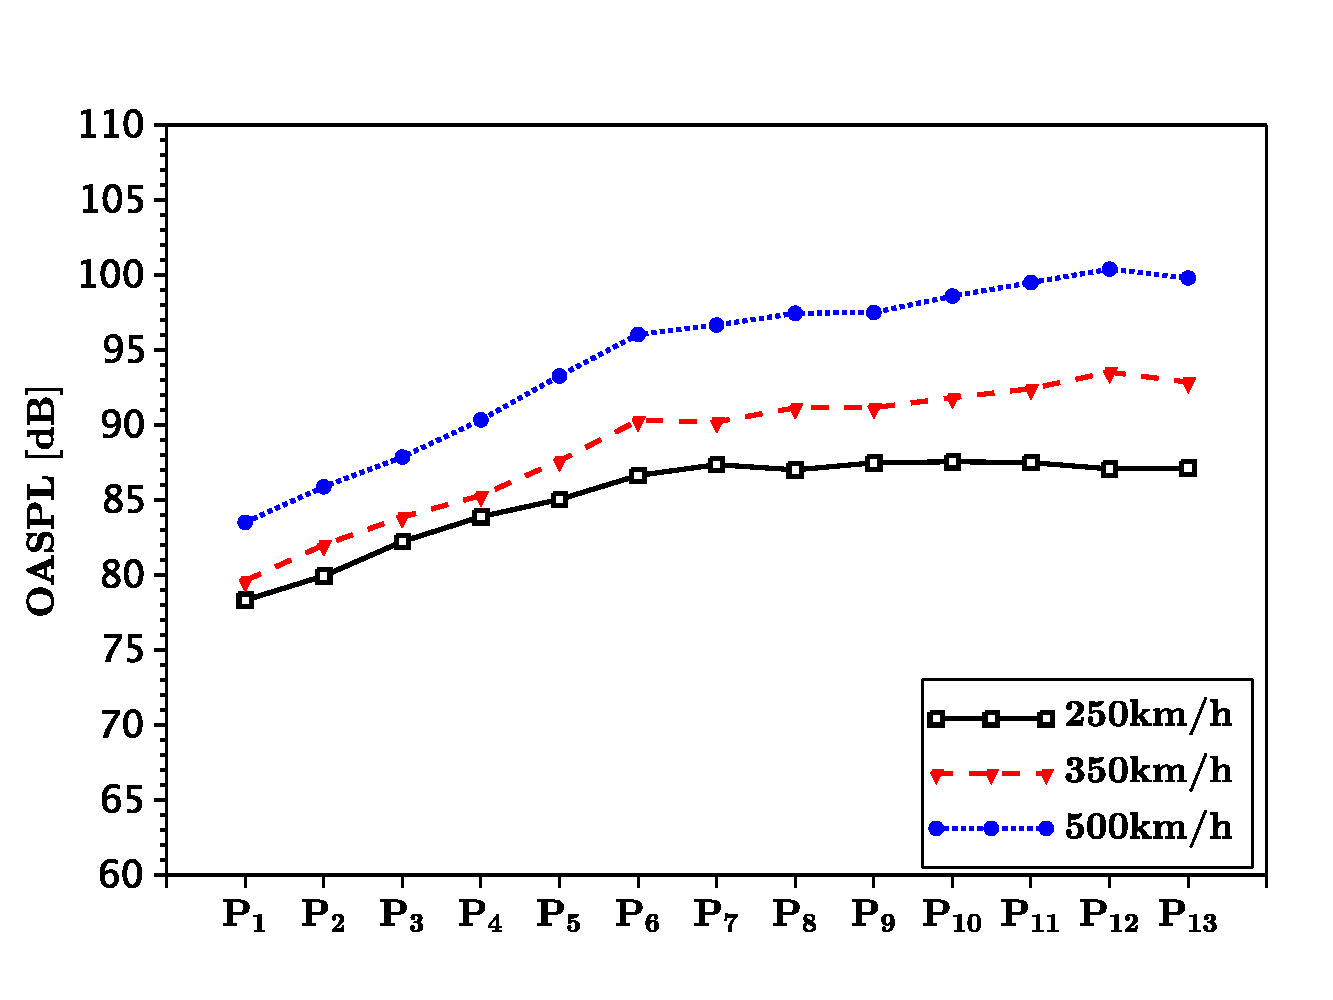
\includegraphics[width=0.55\textwidth]{Figures/oaspl_a.pdf}
  \neufigcaption{fig:ch0-cover}{外部图片插入样例}{Example of Including an External Image}
\end{figure}

\neufigref{fig:ch0-cover} 展示了通过 \verb|\includegraphics| 插入图片文件的方式。
正式论文中建议将图片统一放入 \texttt{Figures} 目录，并使用相对路径引用。

\subsection{PDF 或位图图片}
\begin{figure}[!htbp]
  \centering
  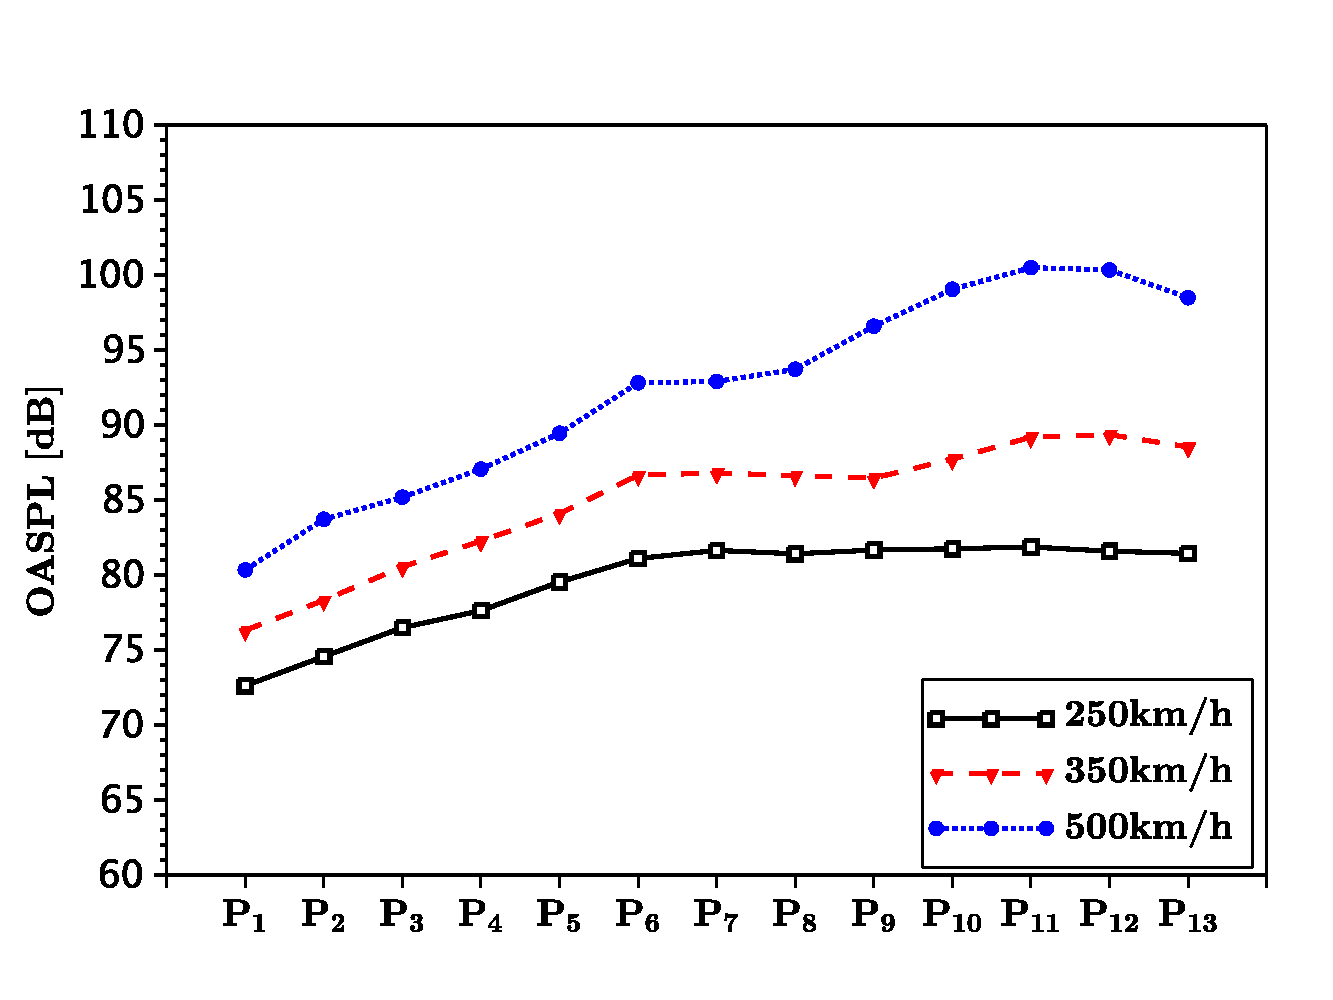
\includegraphics[width=0.55\textwidth]{Figures/oaspl_b.pdf}
  \neufigcaption{fig:ch0-pdf}{PDF 图片插入样例}{Example of Including a PDF Figure}
\end{figure}

PDF、PNG、JPG 等常见图片格式均可通过 \verb|\includegraphics| 插入。
若图片由绘图软件或数据分析程序导出，建议优先使用 PDF 格式以保持较清晰的显示效果。

\subsection{并列图片}
\begin{figure}[!htbp]
  \centering
  \begin{minipage}[t]{0.49\linewidth}
    \centering
    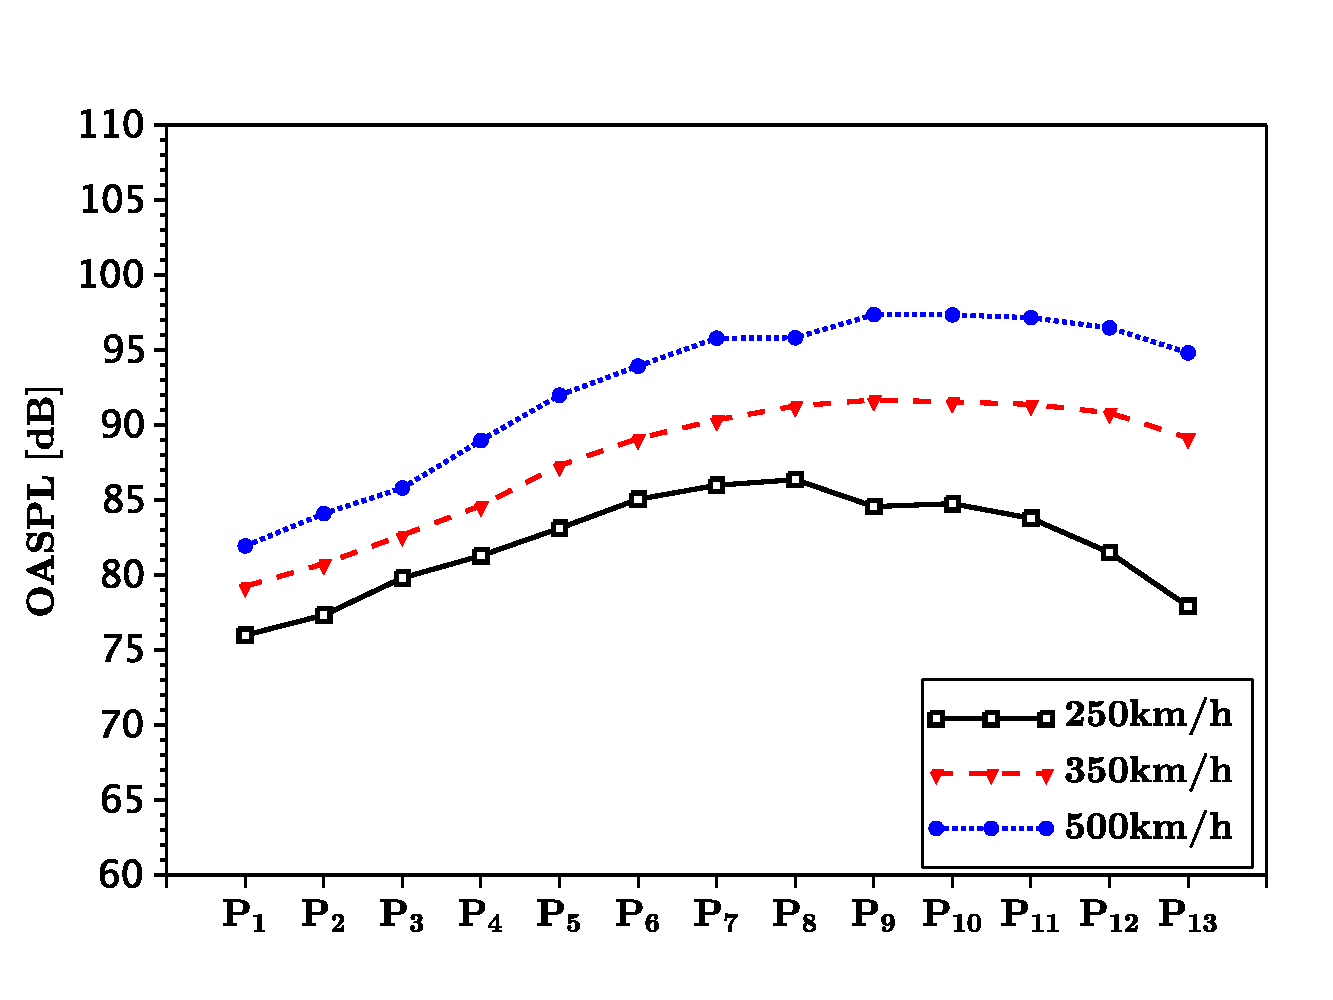
\includegraphics[width=\linewidth]{Figures/oaspl_c.pdf}
  \end{minipage}
  \hfill
  \begin{minipage}[t]{0.49\linewidth}
    \centering
    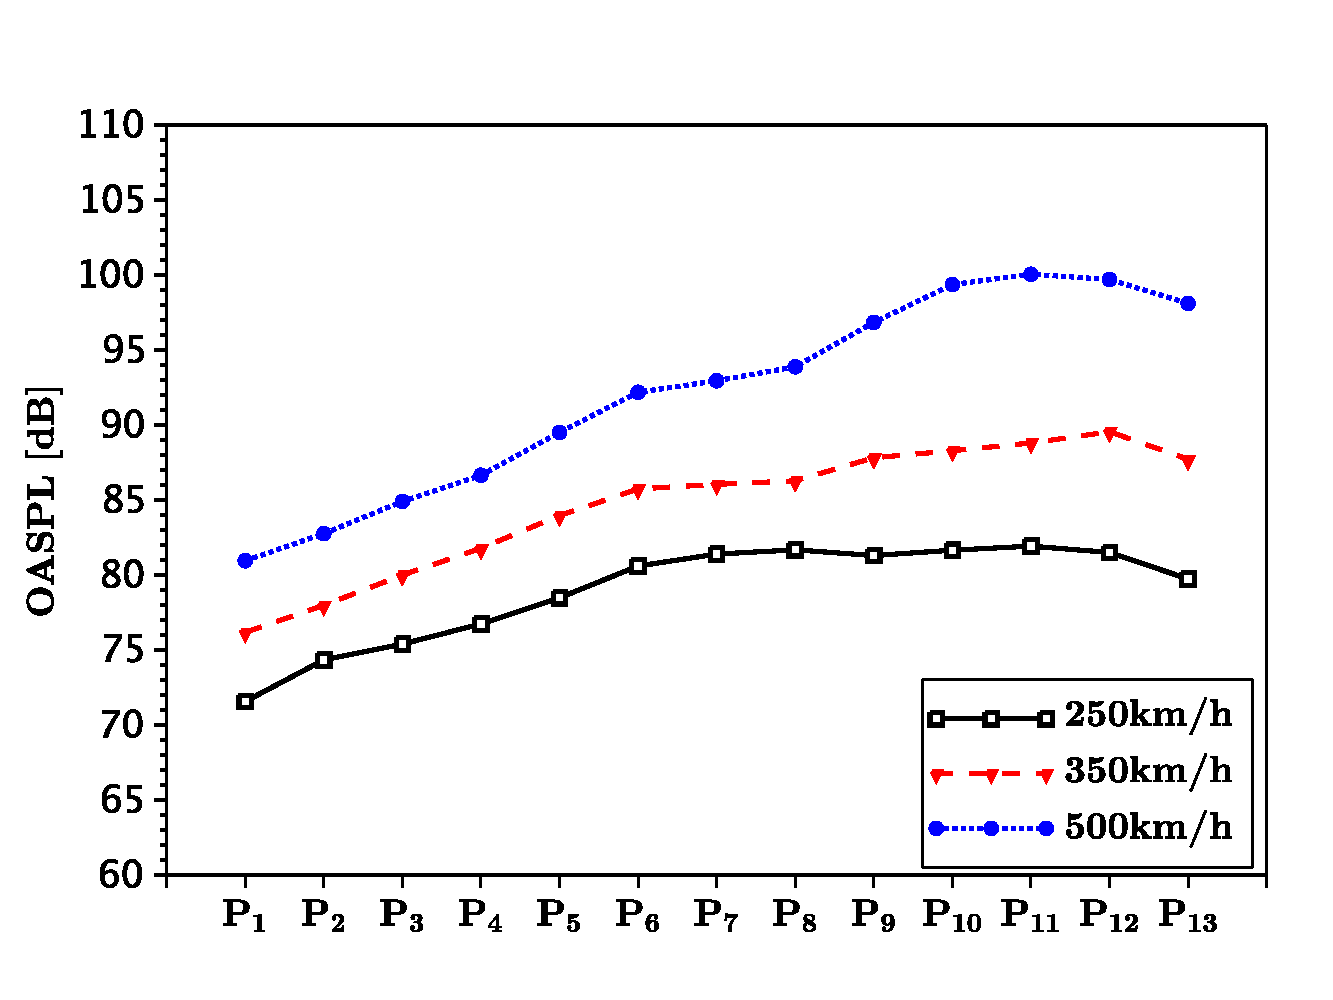
\includegraphics[width=\linewidth]{Figures/oaspl_d.pdf}
  \end{minipage}
  \neufigcaption{fig:ch0-side-by-side}{普通并列图形排版样例}{Example of Side-by-Side Figures}
\end{figure}

\neufigref{fig:ch0-side-by-side} 使用 \texttt{minipage} 完成普通并列排版。
当两幅图共享一个总标题且不需要分别引用时，可使用这种方式。

\subsection{并列子图}
\begin{figure}[!htbp]
  \centering
  \begin{neusubfigure}{0.49\linewidth}
    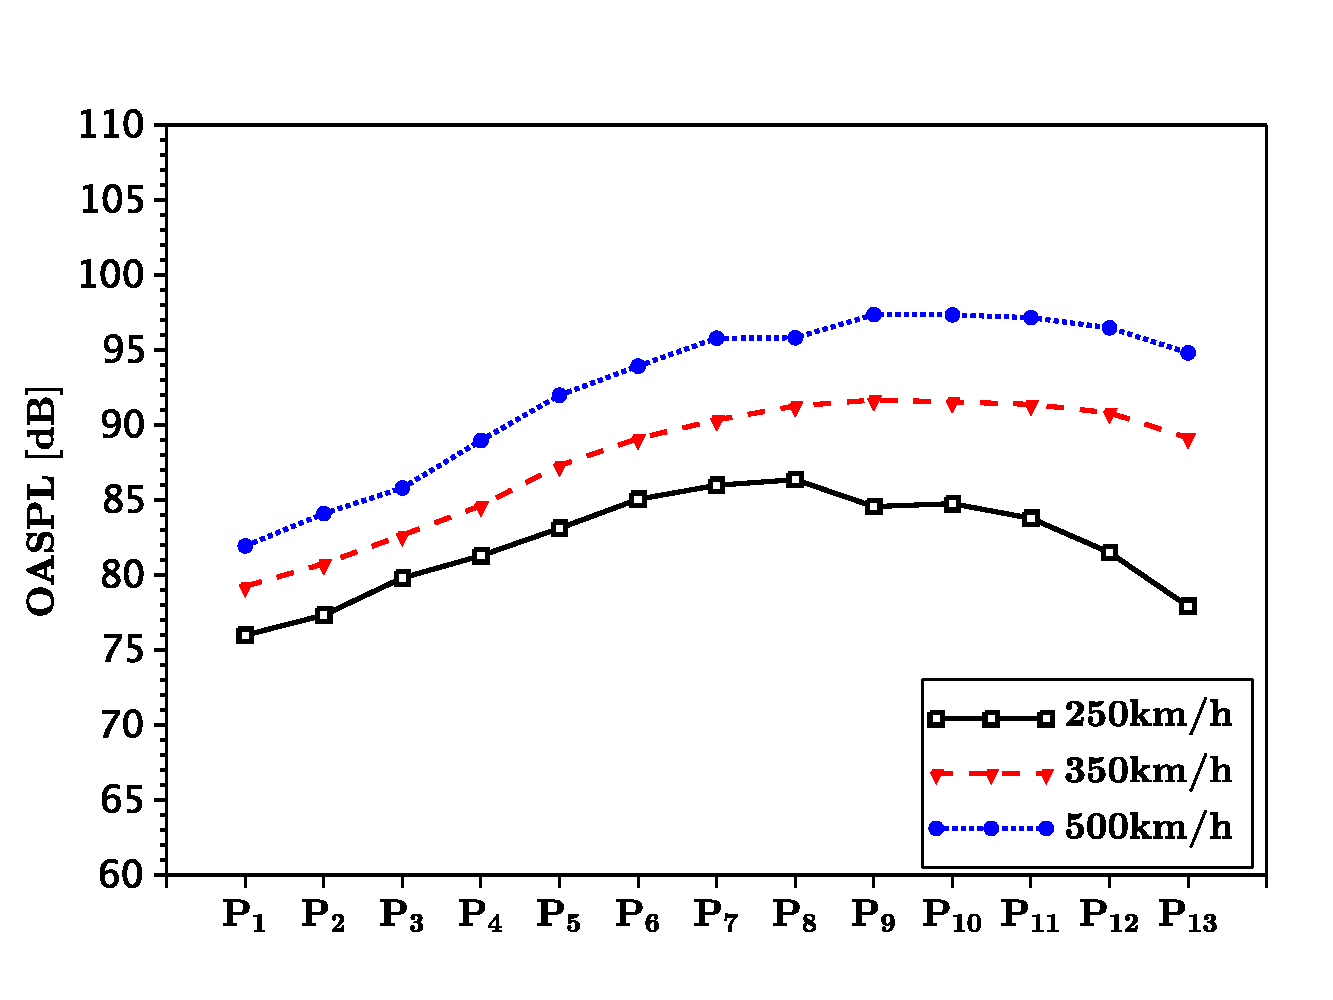
\includegraphics[width=\linewidth]{Figures/oaspl_c.pdf}
    \neusubfigcaption{fig:ch0-side-by-side-a}{工况一}
  \end{neusubfigure}
  \hfill
  \begin{neusubfigure}{0.49\linewidth}
    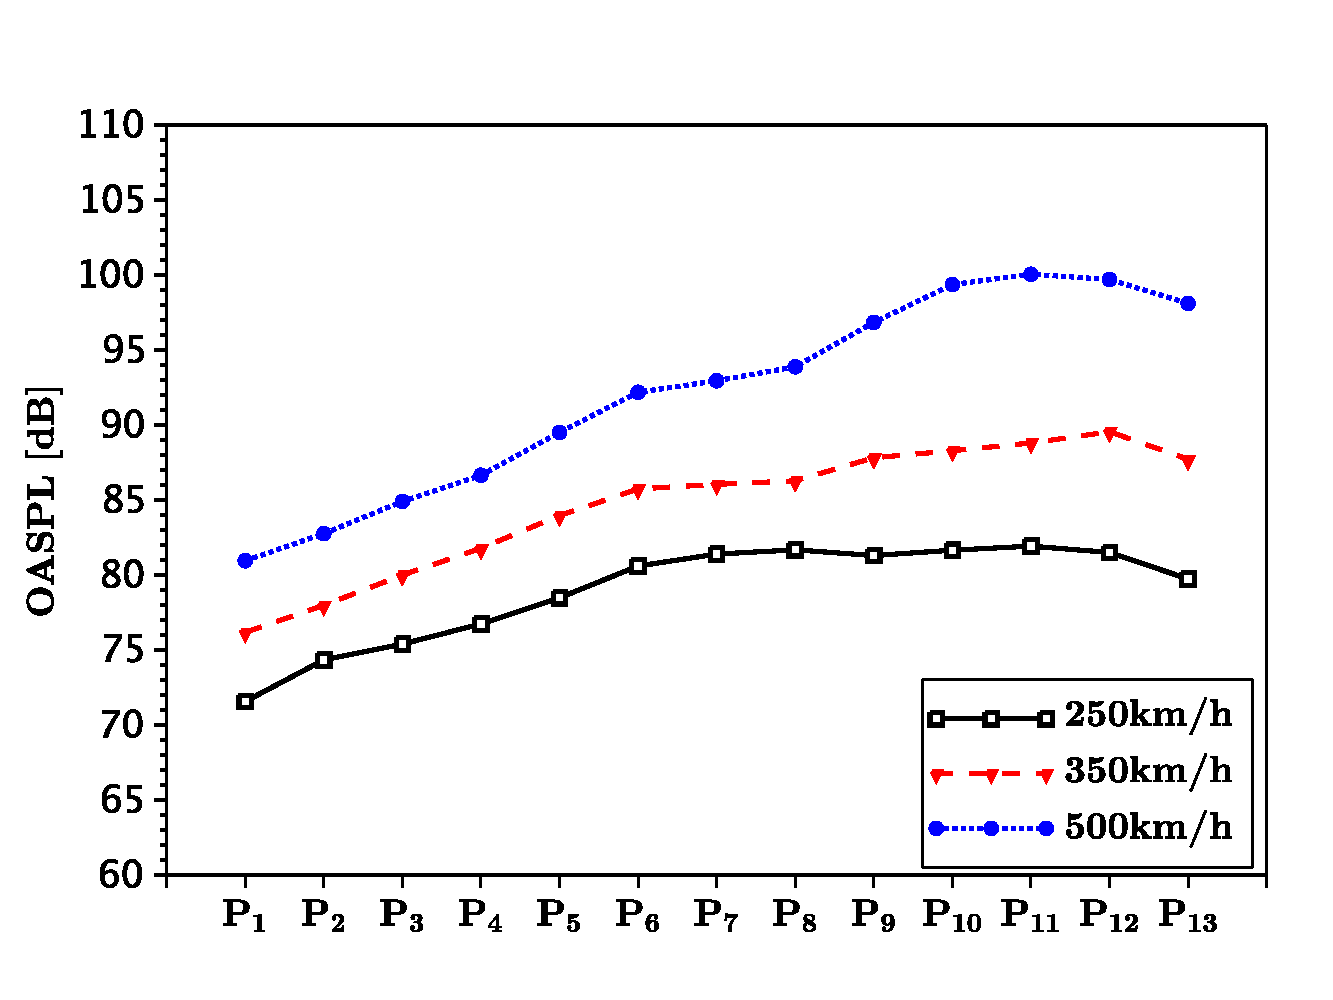
\includegraphics[width=\linewidth]{Figures/oaspl_d.pdf}
    \neusubfigcaption{fig:ch0-side-by-side-b}{工况二}
  \end{neusubfigure}
  \neufigcaption{fig:ch0-subfigures}{并列子图排版样例}{Example of Side-by-Side Subfigures}
\end{figure}

\neufigref{fig:ch0-subfigures} 使用 \texttt{neusubfigure} 完成并列子图排版。
其中 \neusubfigref{fig:ch0-side-by-side-a} 和 \neusubfigref{fig:ch0-side-by-side-b} 可分别引用到子图。
当两幅图共享一个总标题且需要分别引用时，可使用这种方式；如果每幅图需要完全独立的图号，建议拆成两个独立的 \texttt{figure} 环境。

\subsection{二乘二子图}
\begin{figure}[!htbp]
  \centering
  \begin{neusubfigure}{0.49\linewidth}
    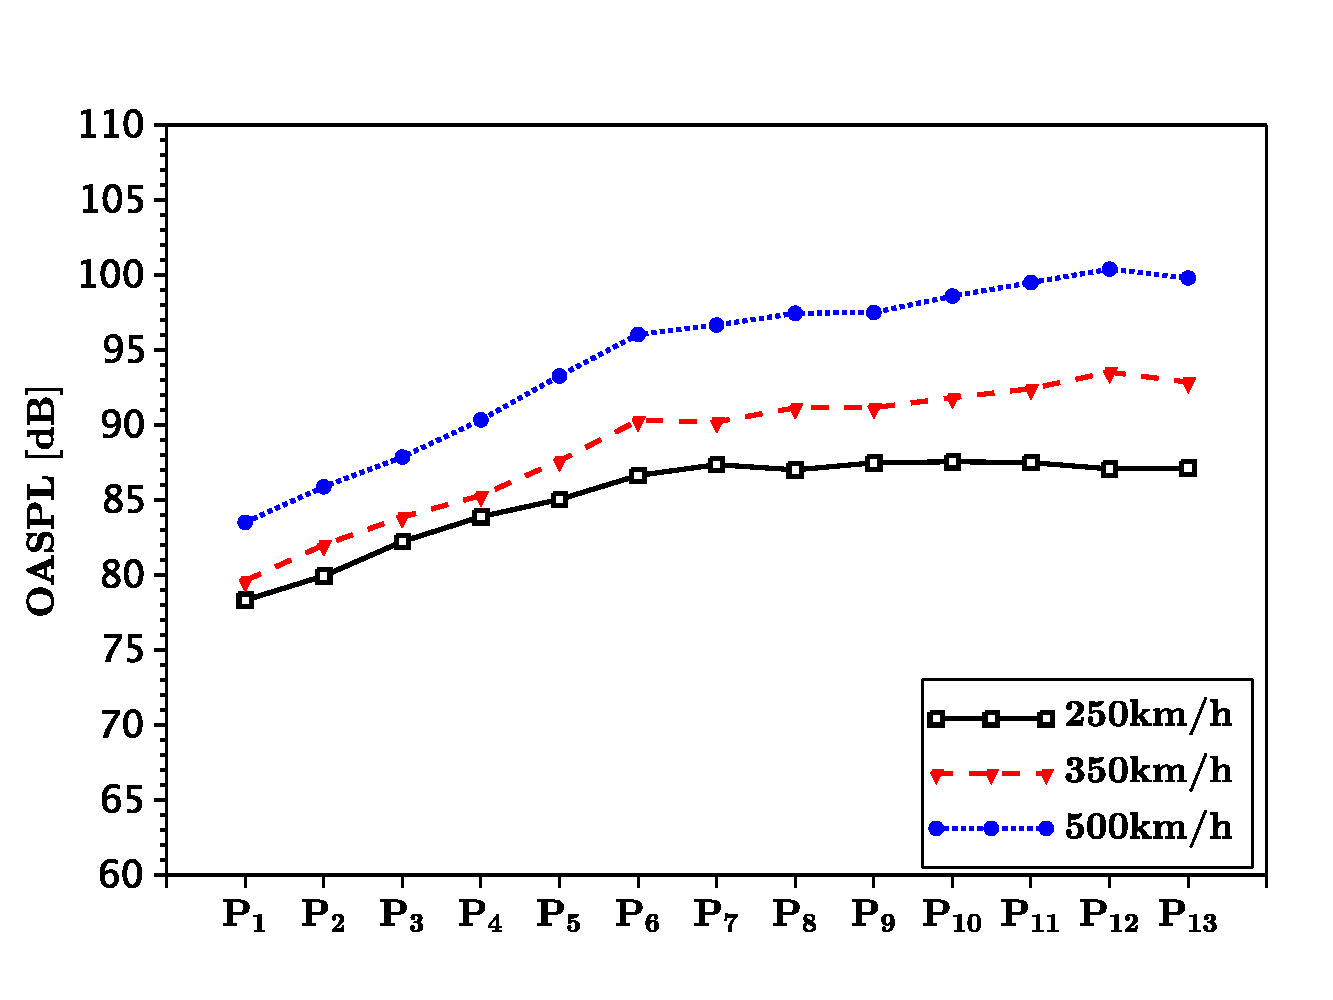
\includegraphics[width=\linewidth]{Figures/oaspl_a.pdf}
    \neusubfigcaption{fig:ch0-four-subfig-a}{工况一}
  \end{neusubfigure}
  \hfill
  \begin{neusubfigure}{0.49\linewidth}
    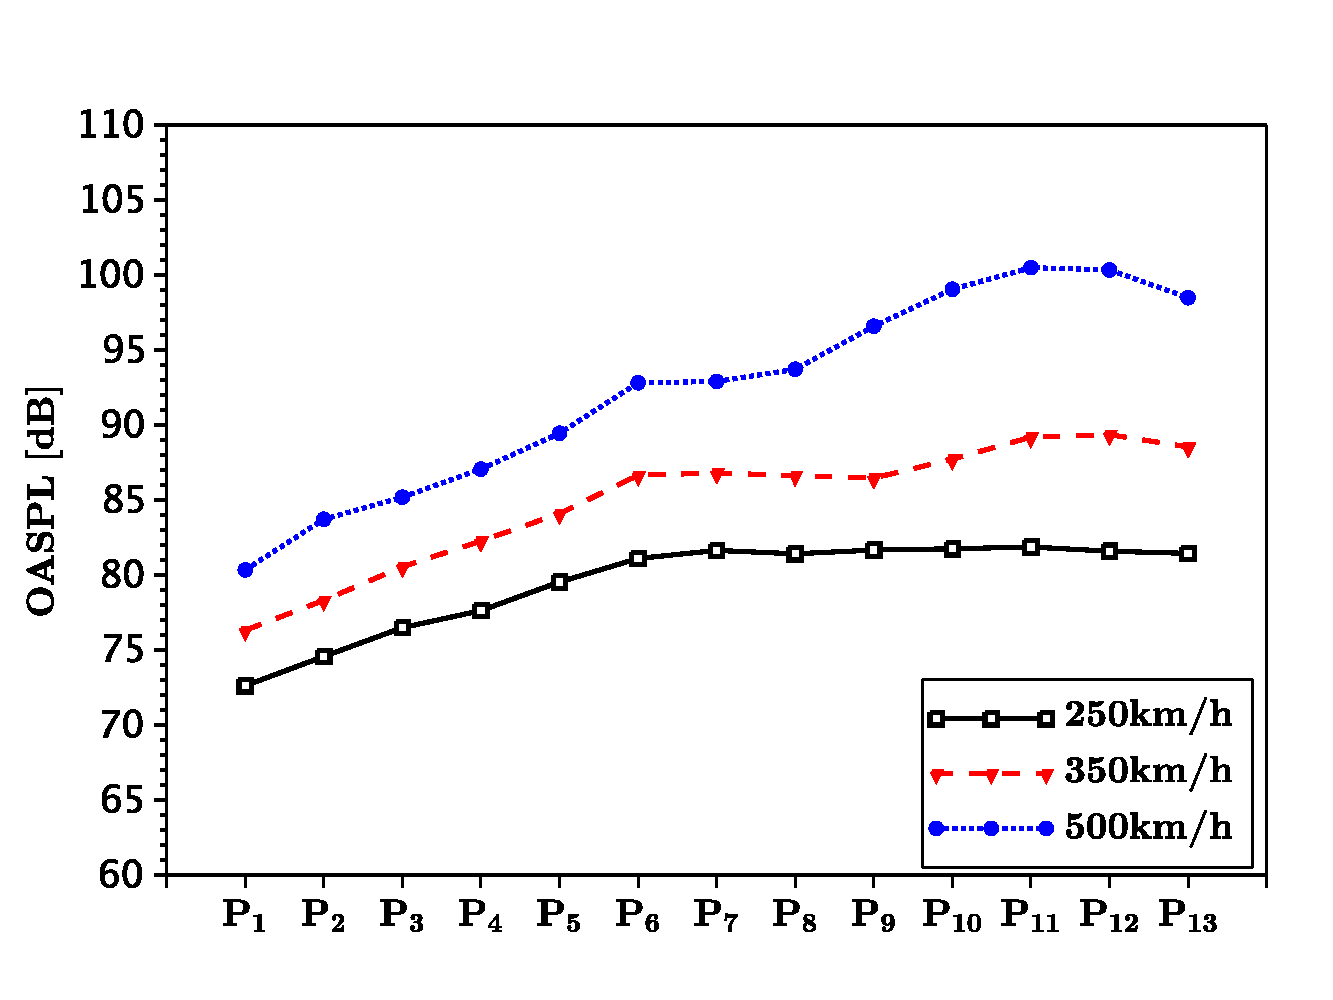
\includegraphics[width=\linewidth]{Figures/oaspl_b.pdf}
    \neusubfigcaption{fig:ch0-four-subfig-b}{工况二}
  \end{neusubfigure}
  \par\vspace{2bp}

  \begin{neusubfigure}{0.49\linewidth}
    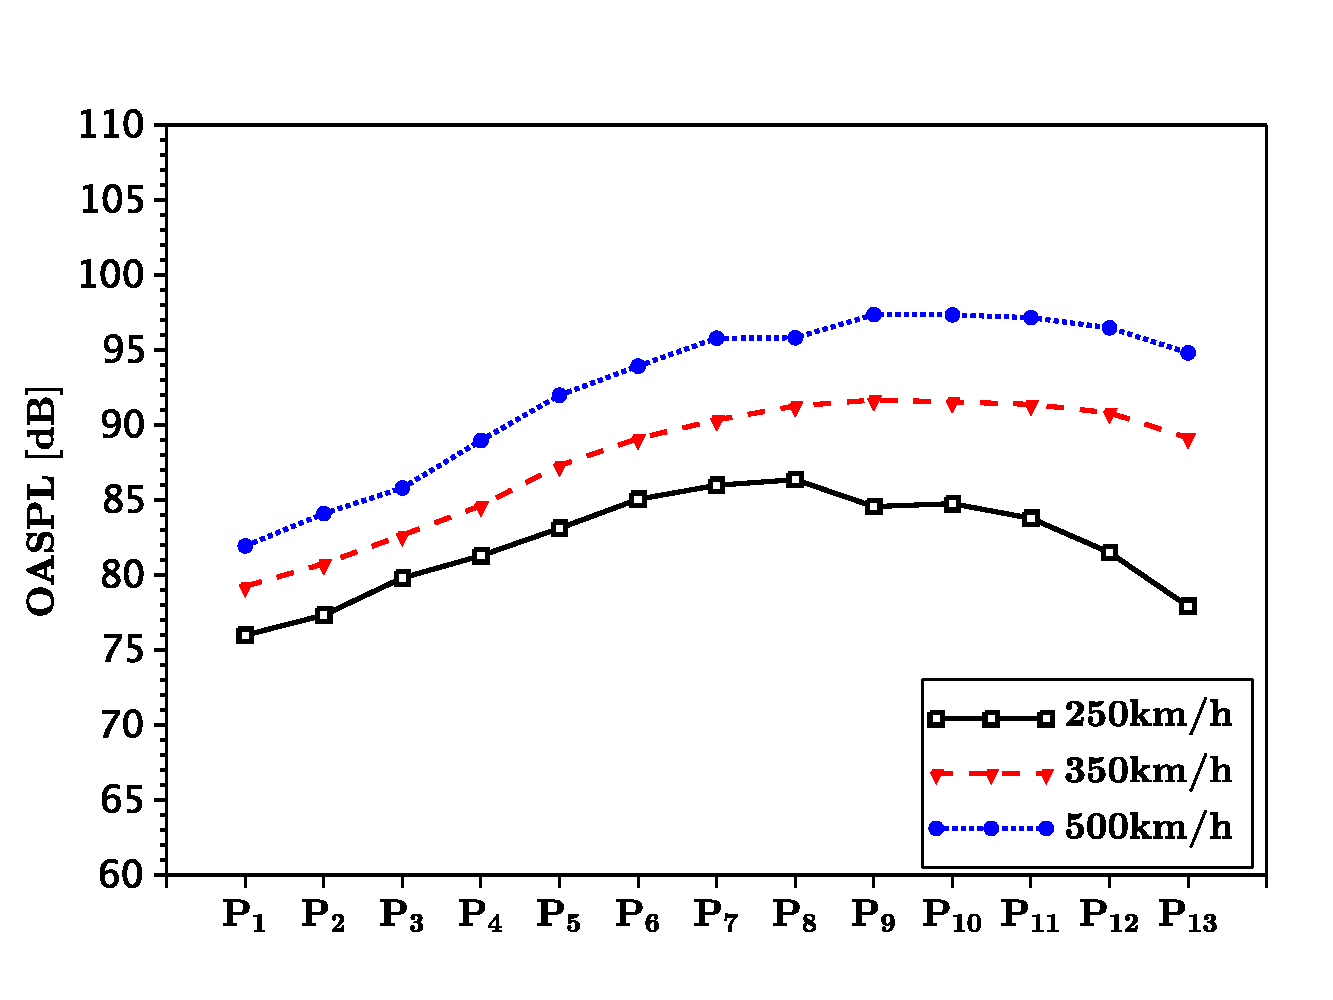
\includegraphics[width=\linewidth]{Figures/oaspl_c.pdf}
    \neusubfigcaption{fig:ch0-four-subfig-c}{工况三}
  \end{neusubfigure}
  \hfill
  \begin{neusubfigure}{0.49\linewidth}
    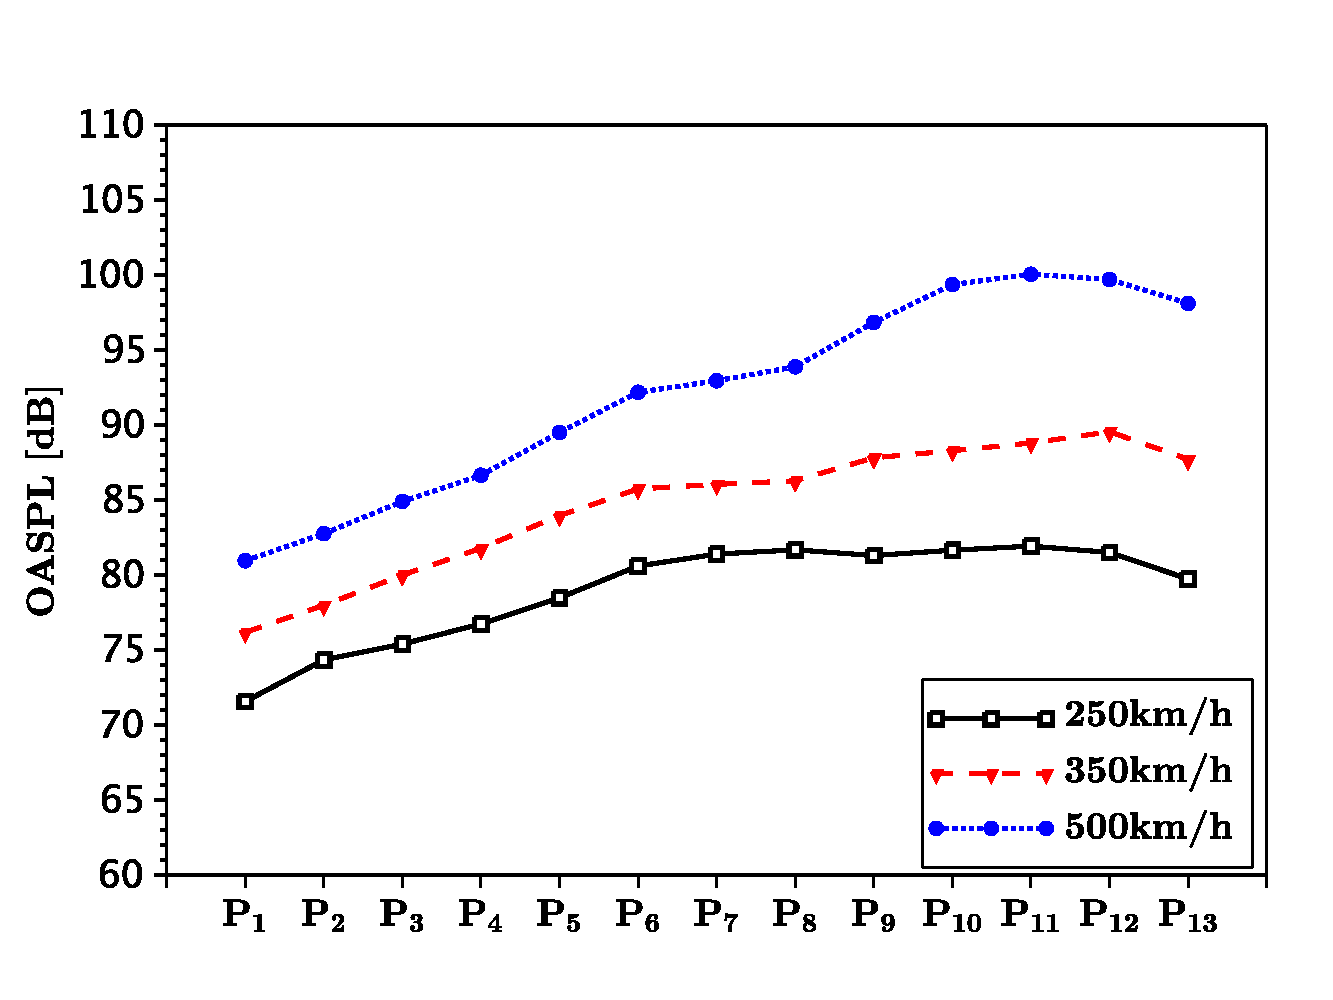
\includegraphics[width=\linewidth]{Figures/oaspl_d.pdf}
    \neusubfigcaption{fig:ch0-four-subfig-d}{工况四}
  \end{neusubfigure}
  \neufigcaption{fig:ch0-four-subfigures}{二乘二子图排版样例}{Example of Two-by-Two Subfigures}
\end{figure}

\neufigref{fig:ch0-four-subfigures} 展示了四幅子图的二乘二排布。
例如 \neusubfigref{fig:ch0-four-subfig-a} 至 \neusubfigref{fig:ch0-four-subfig-d} 可分别引用到四个子图。
排版时建议注意以下几点：
\begin{itemize}
  \item 子图宽度通常可取 \verb|0.48\linewidth| 至 \verb|0.49\linewidth|。
  \item 每行两个子图之间使用 \verb|\hfill| 自动拉开横向间距。
  \item 两行之间可用少量 \verb|\par\vspace| 控制垂直间距。
\end{itemize}

\section{表格排版}

本模板提供 \verb|\neutabcaption{label}{中文题名}{English title}| 用于生成中英文表题。
表题应置于表格上方，正文中使用 \verb|\neutabref{label}| 引用。
表格同样建议使用 \verb|[!htbp]|。如果表格过高导致页底空白，优先考虑缩小字号、调整列宽、拆分表格或使用跨页表格，而不是强制分页。

\subsection{三线表}

\begin{table}[!htbp]
  \centering
  \neutabcaption{tab:ch0-booktabs}{三线表样例}{Example of a Three-Line Table}
  \begin{tabular}{lccc}
    \toprule
    方法       & 准确率（\%）       & 召回率（\%）       & F1 值           \\
    \midrule
    Baseline & 85.2          & 84.1          & 0.846          \\
    Method A & 89.7          & 88.9          & 0.893          \\
    Proposed & \textbf{92.1} & \textbf{91.5} & \textbf{0.918} \\
    \bottomrule
  \end{tabular}
\end{table}

\neutabref{tab:ch0-booktabs} 展示了推荐的三线表格式。
论文中应尽量避免过多竖线，以保持表格简洁。

\subsection{复杂表格}
\begin{table}[!htbp]
  \centering
  \neutabcaption{tab:ch0-complex}{合并单元格与自动换行表格样例}{Example of Merged Cells and Auto-Wrapping Columns}
  \begin{tabularx}{\textwidth}{llXc}
    \toprule
    类别                  & 指标  & 说明                               & 是否必需 \\
    \midrule
    \multirow{2}{*}{图形} & 分辨率 & 位图图片应保证在最终 PDF 中清晰可辨。            & 是    \\
                        & 题名  & 图题使用中英文双语标题，并位于图片下方。             & 是    \\
    \midrule
    \multirow{2}{*}{表格} & 宽度  & 宽表格可使用 \texttt{tabularx} 自动分配列宽。 & 否    \\
                        & 表注  & 表内说明应简明，必要时可在正文中解释。              & 否    \\
    \bottomrule
  \end{tabularx}
\end{table}

\neutabref{tab:ch0-complex} 同时展示了 \verb|\multirow|、\verb|\makecell| 可配合使用的复杂表格场景。
若单元格内容较长，优先使用 \texttt{tabularx} 或 \texttt{p\{...\}} 列类型控制宽度。

\section{公式排版}

公式应使用标准数学环境，并通过 \verb|\label| 设置标签。
引用公式时建议使用模板提供的 \verb|\neueqref{label}|。

\subsection{单行公式}
以分类任务中的交叉熵损失为例，可写为
\begin{equation}
  \mathcal{L}(\theta)
  = - \frac{1}{N}\sum_{i=1}^{N}\sum_{k=1}^{K} y_{ik}\log p_{ik}
  \label{eq:ch0-loss}
\end{equation}

如 \neueqref{eq:ch0-loss} 所示，带编号公式适合放置正文中需要引用的重要定义。

\subsection{多行公式}
循环模型中的状态更新和输出计算可写为
\begin{align}
  h_t       & = \sigma(W_x x_t + W_h h_{t-1} + b), \label{eq:ch0-state} \\
  \hat{y}_t & = \operatorname{softmax}(W_o h_t). \label{eq:ch0-output}
\end{align}

\neueqref{eq:ch0-state} 和 \neueqref{eq:ch0-output} 展示了多行公式的编号方式。
如果多行推导只需要一个编号，可使用 \texttt{aligned} 放在 \texttt{equation} 环境内部。

\subsection{分段函数与矩阵}
分段函数和矩阵经常同时出现在数学定义中，例如
\begin{equation}
  g(x)=
  \begin{cases}
    0, & x < 0,       \\
    x, & 0 \le x < 1, \\
    1, & x \ge 1,
  \end{cases}
  \qquad
  A =
  \begin{bmatrix}
    1 & 0 & 0 \\
    0 & 1 & 0 \\
    0 & 0 & 1
  \end{bmatrix}.
  \label{eq:ch0-piecewise}
\end{equation}

\neueqref{eq:ch0-piecewise} 展示了分段函数和矩阵的常见写法。

\section{算法伪代码}

计算机类论文常需要给出算法步骤。本文档在 \texttt{main.tex} 中加载了 \texttt{algorithm} 和 \texttt{algorithmic} 宏包，可以直接使用如下环境。

\begin{algorithm}[!htbp]
  \caption{样例训练流程}
  \label{alg:ch0-training}
  \begin{algorithmic}[1]
    \REQUIRE Training set $\mathcal{D}$, learning rate $\eta$, maximum epoch $T$
    \ENSURE Model parameters $\theta$
    \STATE Initialize parameters $\theta$
    \FOR{$t = 1$ to $T$}
    \STATE Sample a mini-batch $\mathcal{B}$ from $\mathcal{D}$
    \STATE Compute loss $\mathcal{L}(\theta)$ by \neueqref{eq:ch0-loss}
    \STATE Update $\theta \leftarrow \theta - \eta \nabla_{\theta}\mathcal{L}(\theta)$
    \ENDFOR
    \RETURN $\theta$
  \end{algorithmic}
\end{algorithm}

算法~\ref{alg:ch0-training} 展示了带行号的伪代码。
若需要中文关键字，可在导言区重定义相应命令。

\section{引用、链接与交叉引用}

参考文献引用可使用两种模板命令：
\begin{itemize}
  \item 上标引用使用 \verb|\upcite{key}|，适合放在句末，例如已有研究讨论了神经网络轻量化问题\upcite{guo_2023_research}。
  \item 正文引用使用 \verb|\inlinecite{key}|，适合作为句子成分，例如文献 \inlinecite{thakkar_2018_performance} 给出了系统性能评测案例。
\end{itemize}
多篇文献可写在同一条引用命令中，例如区块链平台相关研究\upcite{zheng_2019_nutbaas,thakkar_2018_performance}。

交叉引用建议统一使用模板命令：
\begin{itemize}
  \item 图引用：\verb|\neufigref{fig:ch0-pdf}|，效果为 \neufigref{fig:ch0-pdf}。
  \item 子图引用：\verb|\neusubfigref{fig:ch0-four-subfig-a}|，效果为 \neusubfigref{fig:ch0-four-subfig-a}。
  \item 表引用：\verb|\neutabref{tab:ch0-complex}|，效果为 \neutabref{tab:ch0-complex}。
  \item 公式引用：\verb|\neueqref{eq:ch0-loss}|，效果为 \neueqref{eq:ch0-loss}。
  \item 算法引用：当前模板未单独封装算法引用命令，可写作“算法~\ref{alg:ch0-training}”。
\end{itemize}
模板提供的公开命令和环境可参考 \texttt{README.md} 中的“模板命令说明”一节。
|。
脚注示例如此处所示\footnote{脚注用于补充说明，不宜放置过长的正文内容。}。
若某页因图表浮动或分页规则没有排满，脚注可能跟随正文排版区而显得略高，这是正常的 LaTeX 页面构建结果。

\subsection{字体、字号与强调}

模板预定义了常用中文字体命令。正式论文中通常不需要手动切换字体；只有在展示样式、术语强调或特殊说明时才建议使用。
当前模板已经为默认宋体和 \verb|\song| 字族配置伪粗体，因此 \verb|\textbf| 或 \verb|\bfseries| 可以用于中文局部强调。
需要注意的是，中文加粗应克制使用；标题层级、术语定义或表格重点值可以适当加粗，大段正文不建议整体加粗。
如果需要更明显的标题式强调，可使用黑体或调整标题层级；如果只是普通正文重点，优先使用 \verb|\textbf|。

\begin{table}[!htbp]
  \centering
  \neutabcaption{tab:ch0-fonts}{字体与强调样例}{Examples of Fonts and Emphasis}
  \begin{tabular}{lll}
    \toprule
    命令             & 显示效果                         & 使用建议       \\
    \midrule
    \verb|\song|   & {\song 宋体文字示例}               & 正文默认字体     \\
    \verb|\textbf| & \textbf{加粗文字示例}              & 局部强调、表格重点值 \\
    \verb|\hei|    & {\hei 黑体文字示例}                & 标题或较强强调场景  \\
    \verb|\kai|    & {\kai 楷体文字示例}                & 摘要、题签或引用语  \\
    \verb|\fs|     & {\fs 仿宋文字示例}                 & 特殊文书类内容    \\
    \verb|\textit| & \textit{Italic text example} & 英文斜体或变量说明  \\
    \bottomrule
  \end{tabular}
\end{table}

\subsection{列表环境}

无序列表适合列出并列事项：
\begin{itemize}
  \item 图题位于图下方，表题位于表上方。
  \item 图表应使用中英文双语标题。
  \item 公式、图、表、算法均应使用标签进行交叉引用。
\end{itemize}

有序列表适合描述步骤：
\begin{enumerate}
  \item 在 \texttt{main.tex} 中填写论文元信息。
  \item 在各章文件中撰写正文内容。
  \item 使用 \texttt{latexmk -xelatex main.tex} 完成编译。
\end{enumerate}

\section{图形排版}

本模板提供 \verb|\neufigcaption{label}{中文题名}{English title}| 用于生成中英文图题。
图题应置于图形下方，正文中使用 \verb|\neufigref{label}| 引用。
图形建议使用 \verb|[!htbp]| 浮动参数，让 LaTeX 在当前位置、页顶、页底或浮动页中选择较合适的位置；除非必须固定位置，否则不建议使用 \verb|[H]|。

\subsection{外部图片}
\begin{figure}[!htbp]
  \centering
  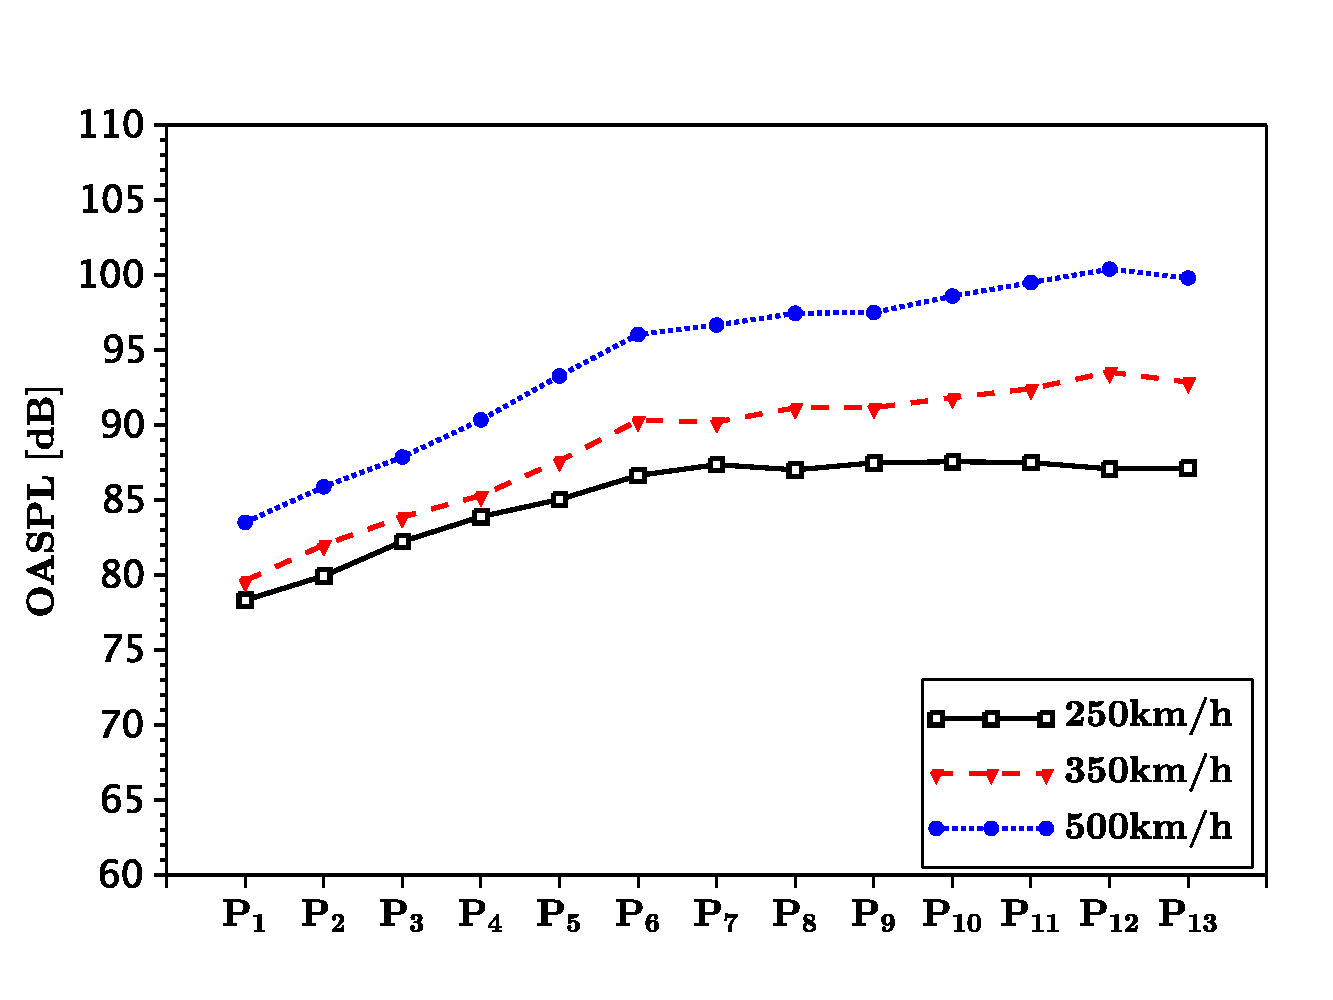
\includegraphics[width=0.55\textwidth]{Figures/oaspl_a.pdf}
  \neufigcaption{fig:ch0-cover}{外部图片插入样例}{Example of Including an External Image}
\end{figure}

\neufigref{fig:ch0-cover} 展示了通过 \verb|\includegraphics| 插入图片文件的方式。
正式论文中建议将图片统一放入 \texttt{Figures} 目录，并使用相对路径引用。

\subsection{PDF 或位图图片}
\begin{figure}[!htbp]
  \centering
  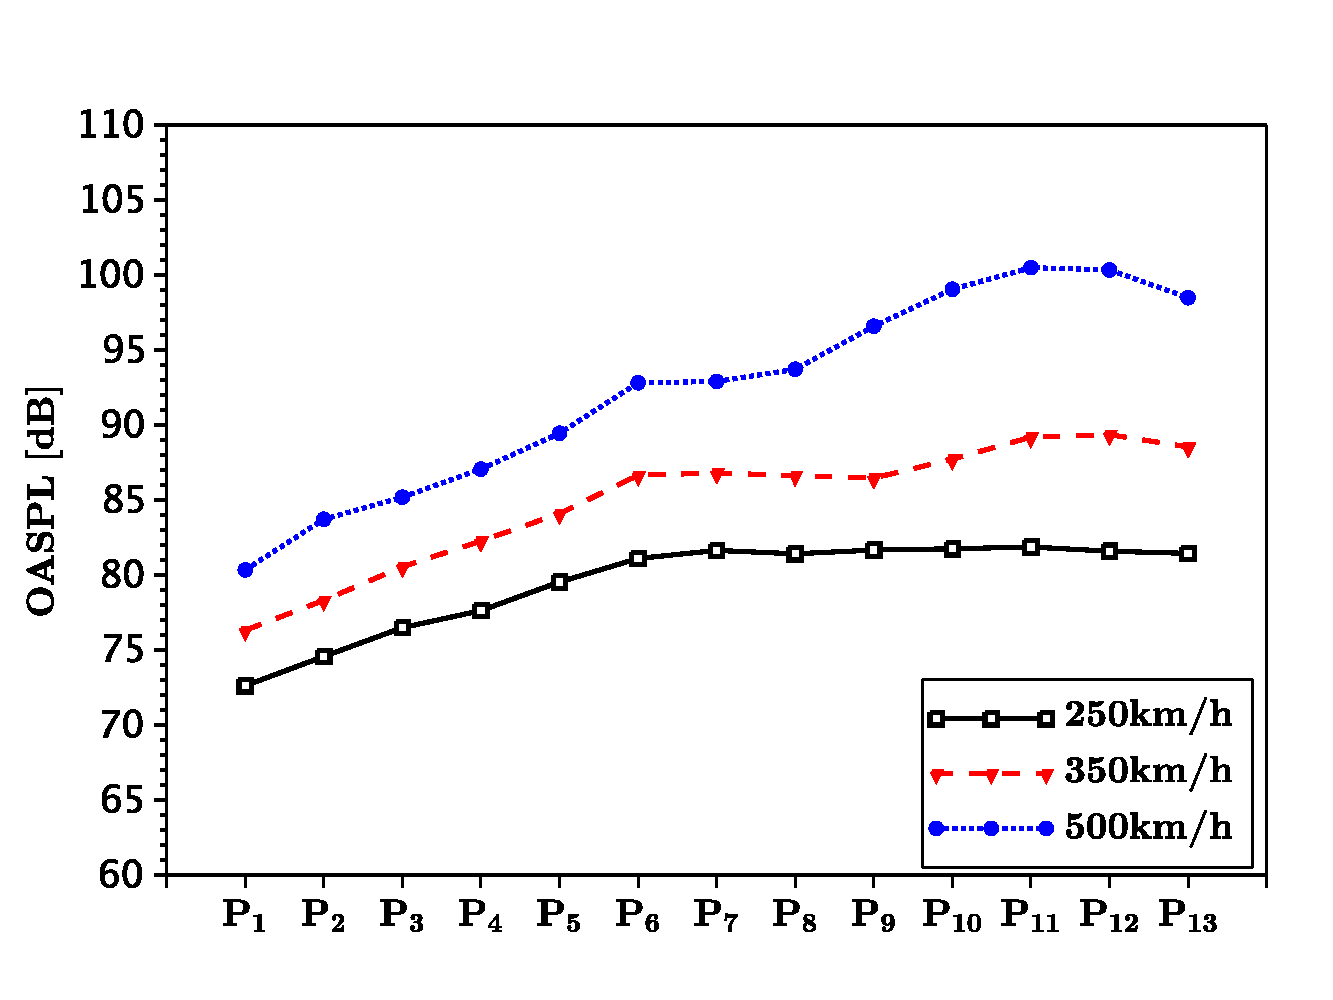
\includegraphics[width=0.55\textwidth]{Figures/oaspl_b.pdf}
  \neufigcaption{fig:ch0-pdf}{PDF 图片插入样例}{Example of Including a PDF Figure}
\end{figure}

PDF、PNG、JPG 等常见图片格式均可通过 \verb|\includegraphics| 插入。
若图片由绘图软件或数据分析程序导出，建议优先使用 PDF 格式以保持较清晰的显示效果。

\subsection{并列图片}
\begin{figure}[!htbp]
  \centering
  \begin{minipage}[t]{0.49\linewidth}
    \centering
    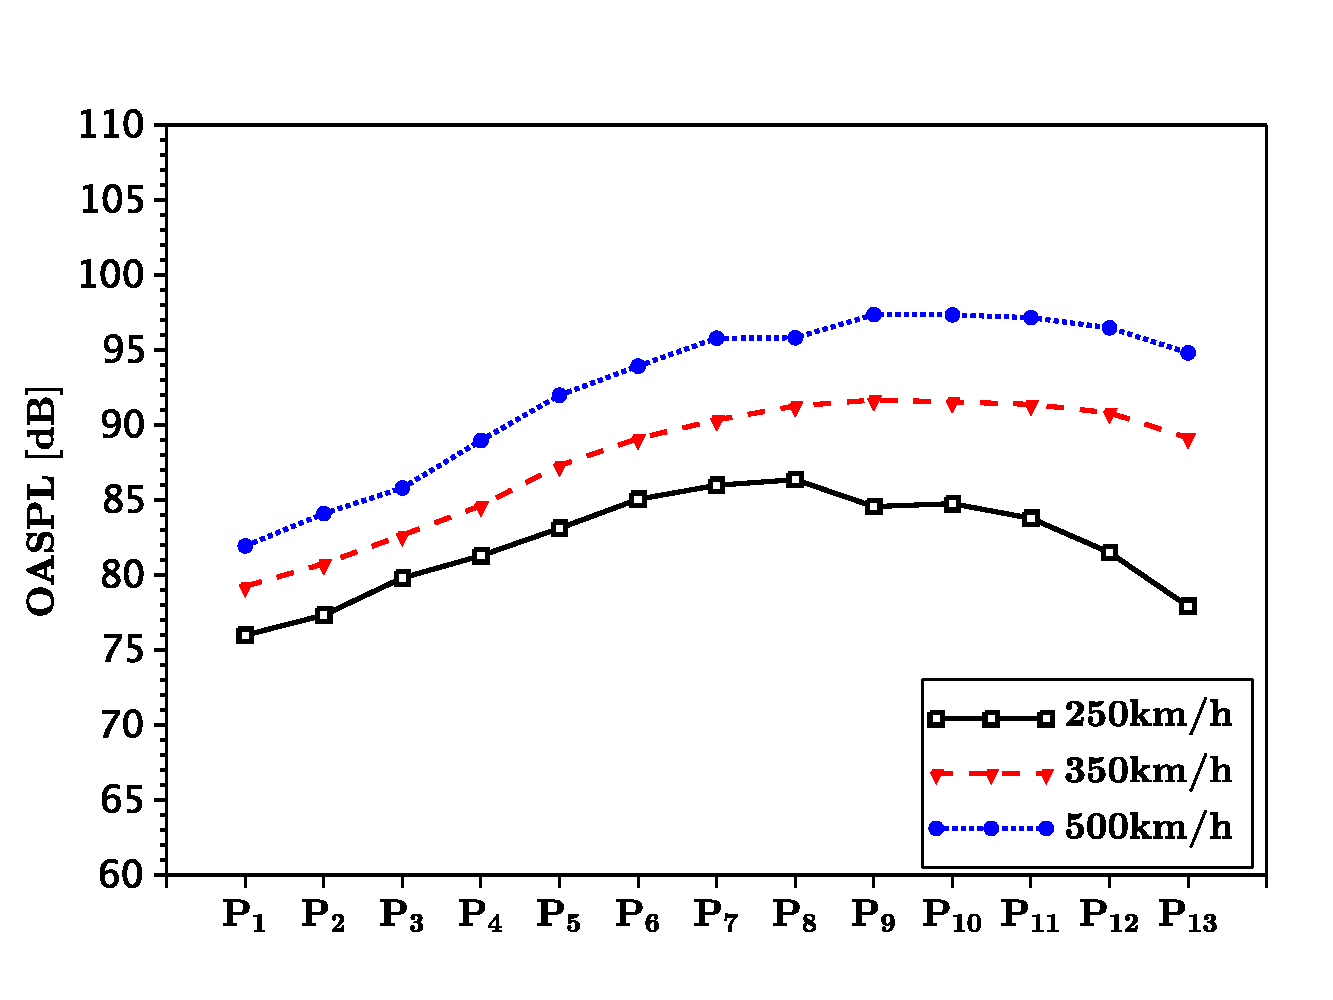
\includegraphics[width=\linewidth]{Figures/oaspl_c.pdf}
  \end{minipage}
  \hfill
  \begin{minipage}[t]{0.49\linewidth}
    \centering
    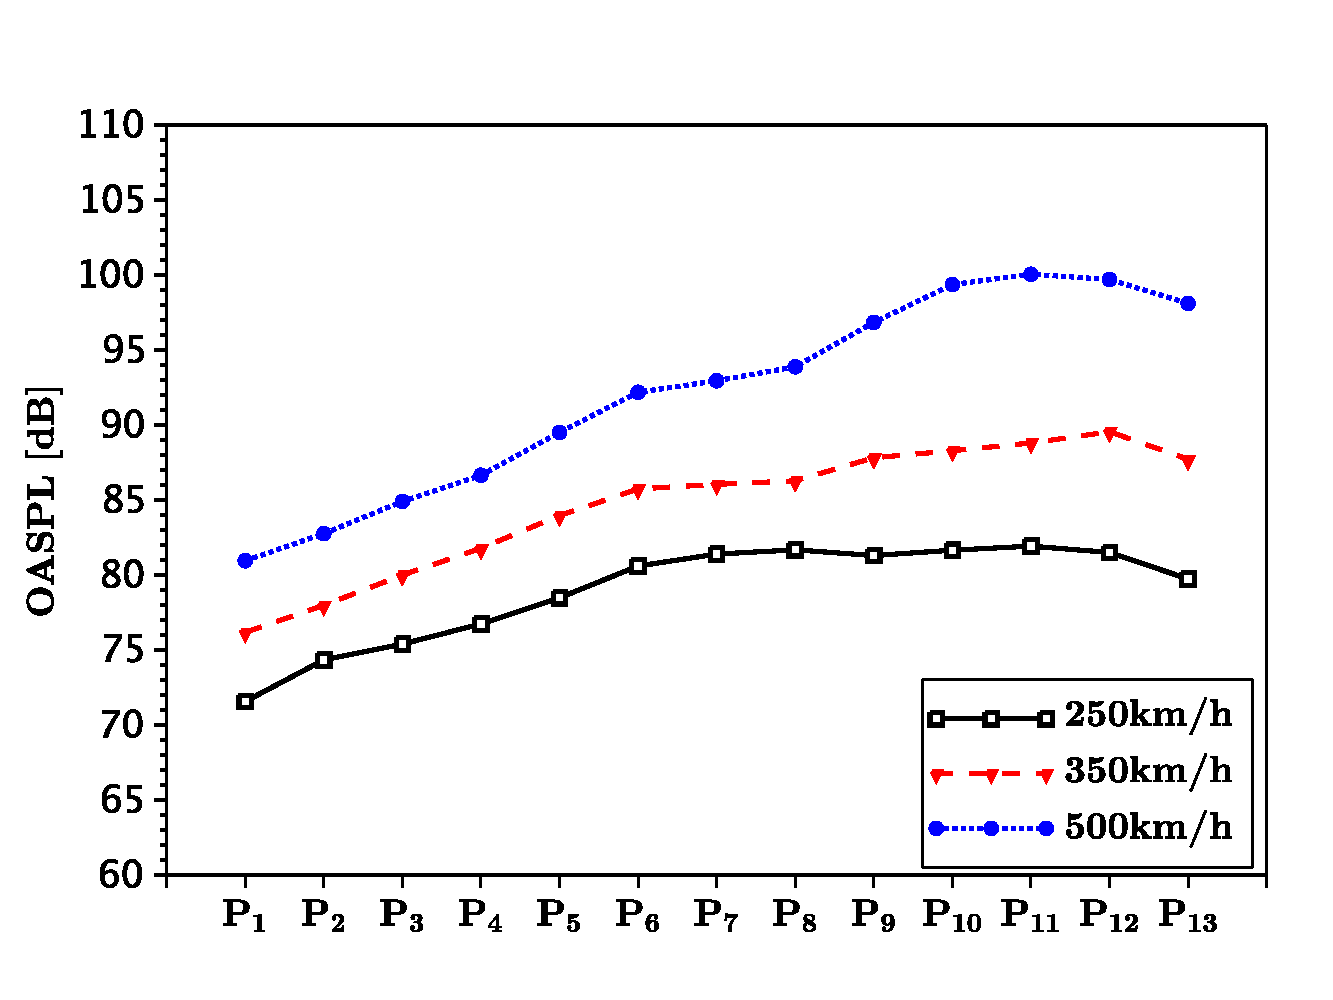
\includegraphics[width=\linewidth]{Figures/oaspl_d.pdf}
  \end{minipage}
  \neufigcaption{fig:ch0-side-by-side}{普通并列图形排版样例}{Example of Side-by-Side Figures}
\end{figure}

\neufigref{fig:ch0-side-by-side} 使用 \texttt{minipage} 完成普通并列排版。
当两幅图共享一个总标题且不需要分别引用时，可使用这种方式。

\subsection{并列子图}
\begin{figure}[!htbp]
  \centering
  \begin{neusubfigure}{0.49\linewidth}
    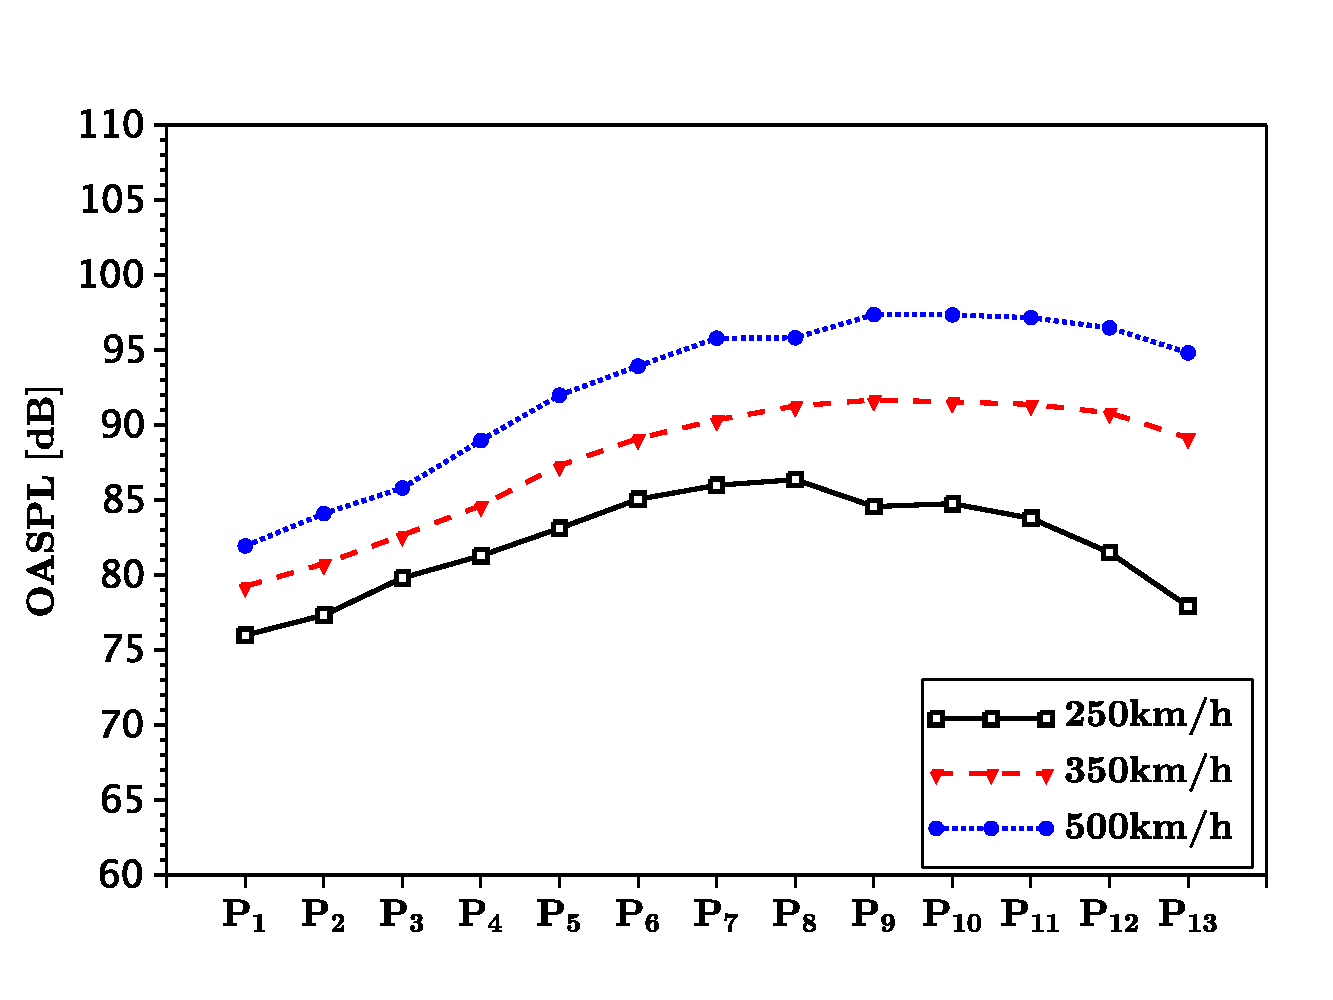
\includegraphics[width=\linewidth]{Figures/oaspl_c.pdf}
    \neusubfigcaption{fig:ch0-side-by-side-a}{工况一}
  \end{neusubfigure}
  \hfill
  \begin{neusubfigure}{0.49\linewidth}
    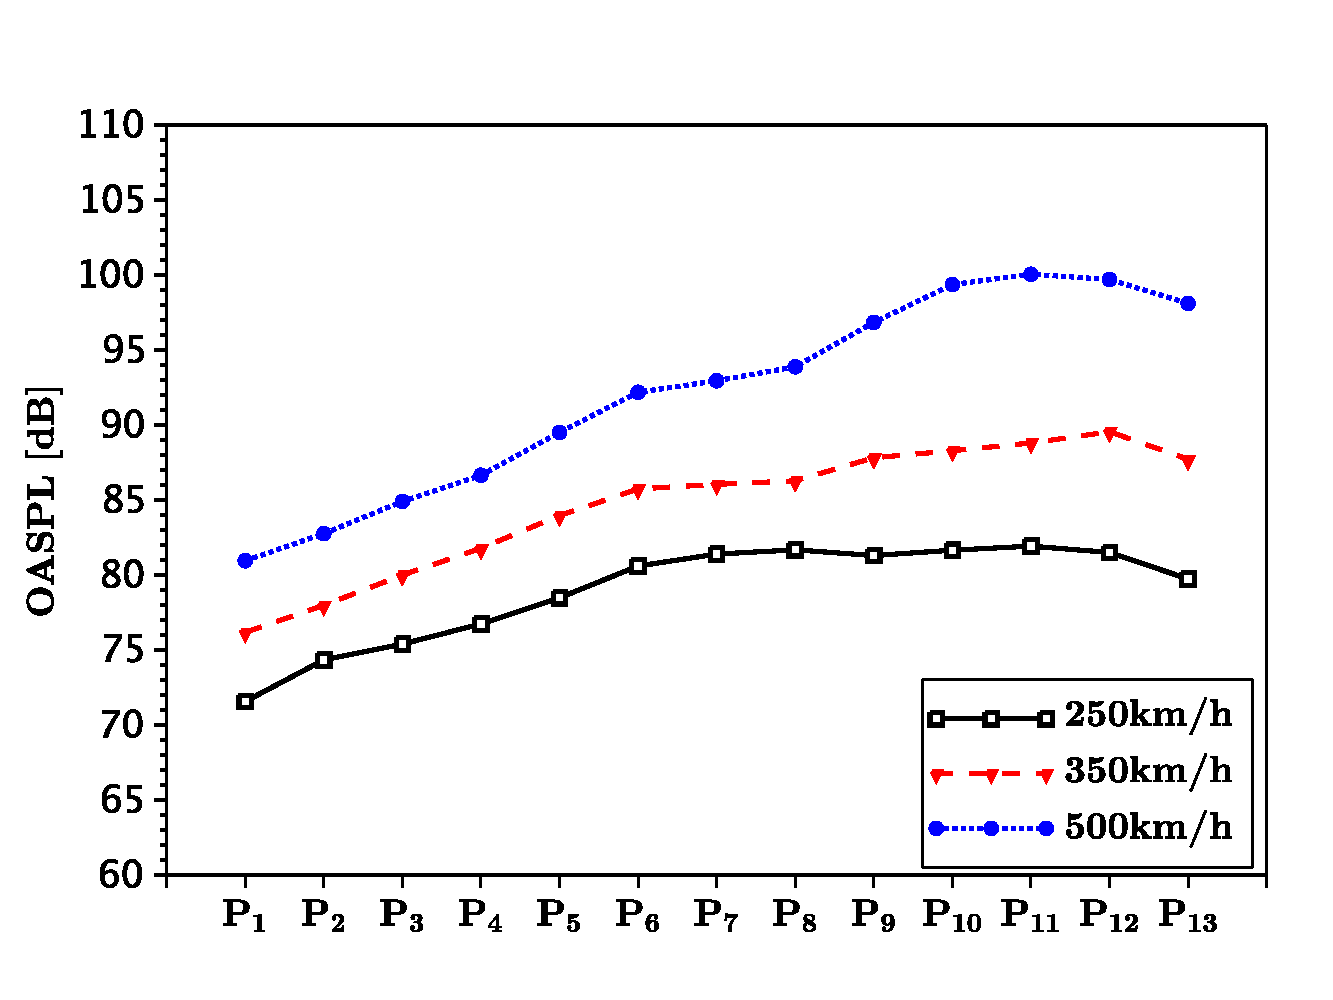
\includegraphics[width=\linewidth]{Figures/oaspl_d.pdf}
    \neusubfigcaption{fig:ch0-side-by-side-b}{工况二}
  \end{neusubfigure}
  \neufigcaption{fig:ch0-subfigures}{并列子图排版样例}{Example of Side-by-Side Subfigures}
\end{figure}

\neufigref{fig:ch0-subfigures} 使用 \texttt{neusubfigure} 完成并列子图排版。
其中 \neusubfigref{fig:ch0-side-by-side-a} 和 \neusubfigref{fig:ch0-side-by-side-b} 可分别引用到子图。
当两幅图共享一个总标题且需要分别引用时，可使用这种方式；如果每幅图需要完全独立的图号，建议拆成两个独立的 \texttt{figure} 环境。

\subsection{二乘二子图}
\begin{figure}[!htbp]
  \centering
  \begin{neusubfigure}{0.49\linewidth}
    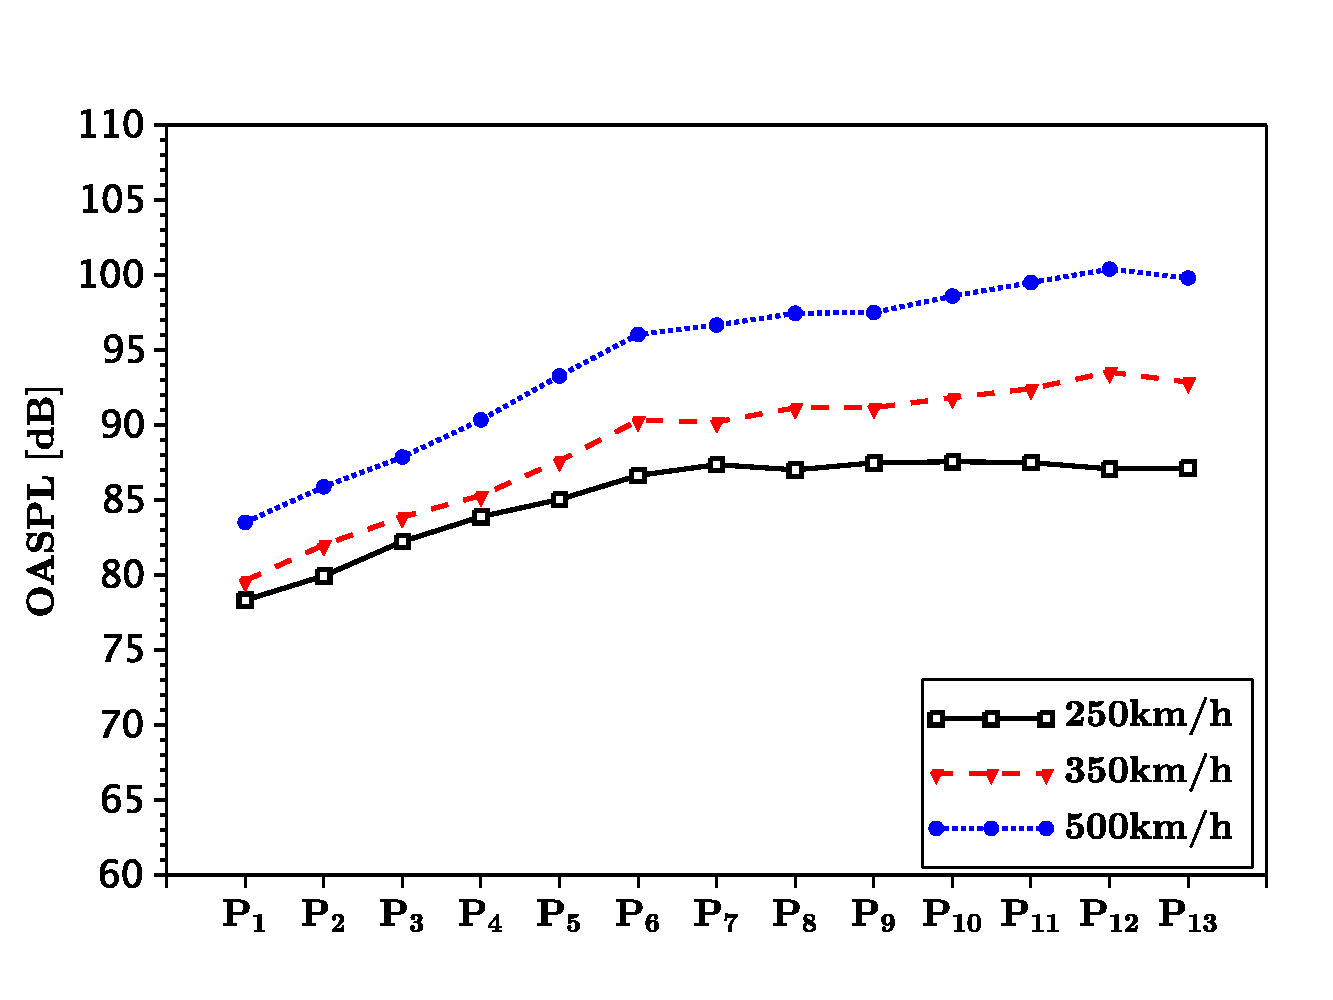
\includegraphics[width=\linewidth]{Figures/oaspl_a.pdf}
    \neusubfigcaption{fig:ch0-four-subfig-a}{工况一}
  \end{neusubfigure}
  \hfill
  \begin{neusubfigure}{0.49\linewidth}
    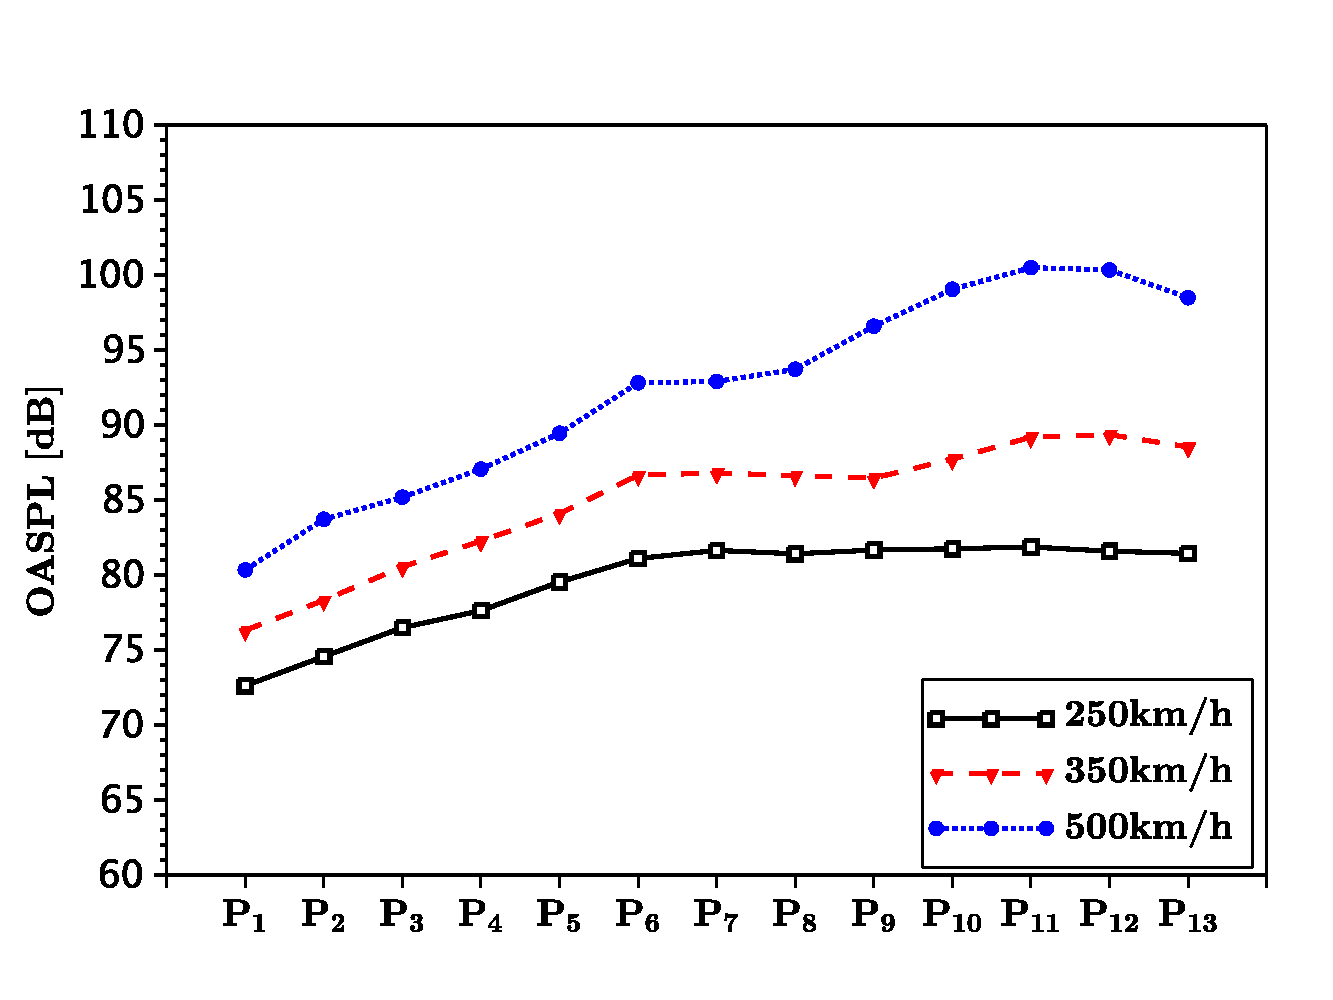
\includegraphics[width=\linewidth]{Figures/oaspl_b.pdf}
    \neusubfigcaption{fig:ch0-four-subfig-b}{工况二}
  \end{neusubfigure}
  \par\vspace{2bp}

  \begin{neusubfigure}{0.49\linewidth}
    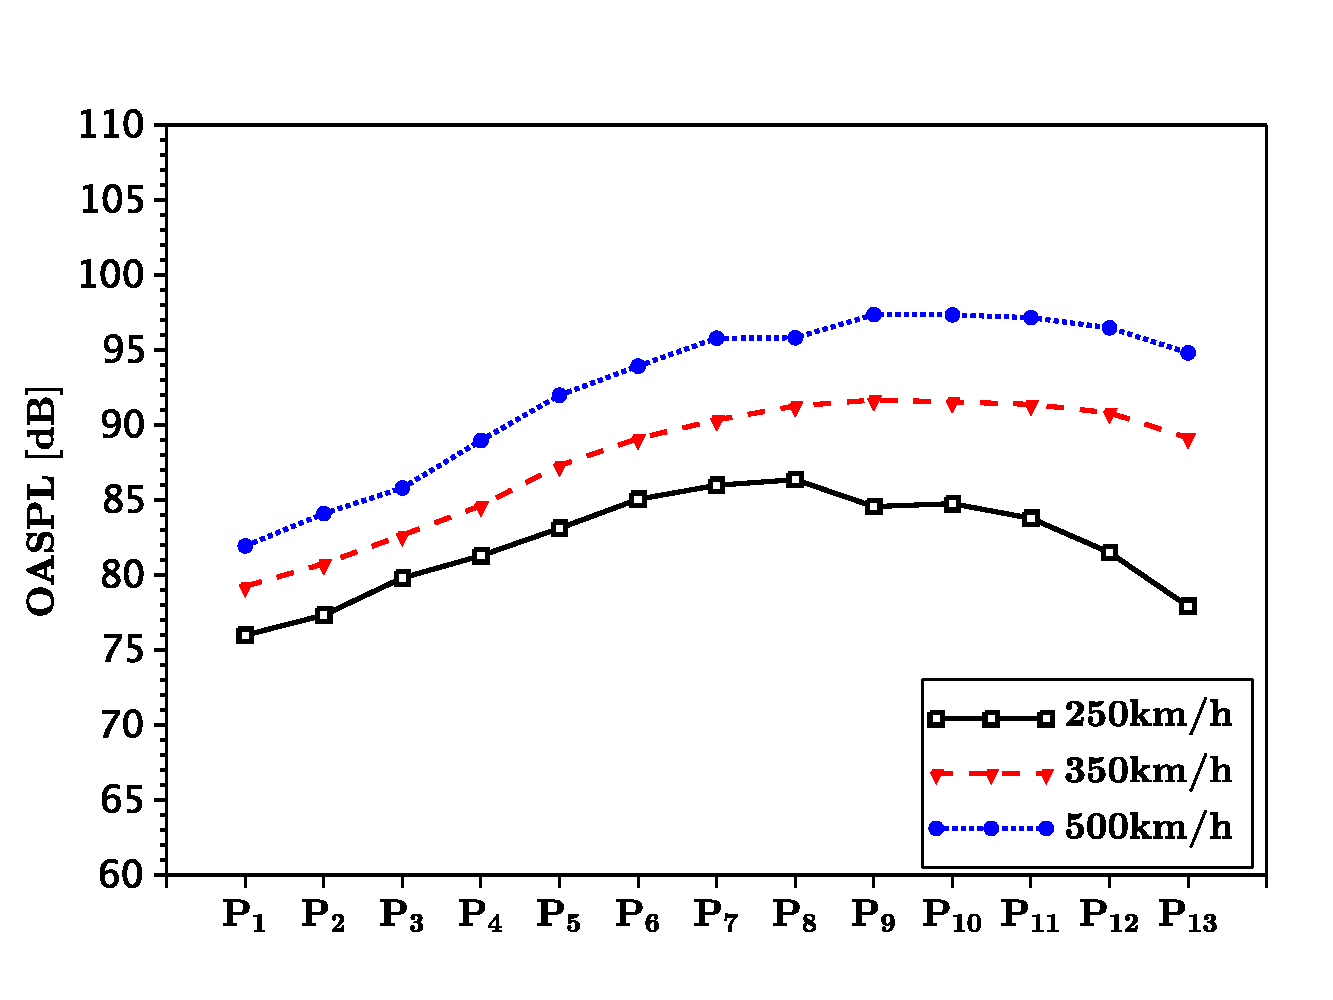
\includegraphics[width=\linewidth]{Figures/oaspl_c.pdf}
    \neusubfigcaption{fig:ch0-four-subfig-c}{工况三}
  \end{neusubfigure}
  \hfill
  \begin{neusubfigure}{0.49\linewidth}
    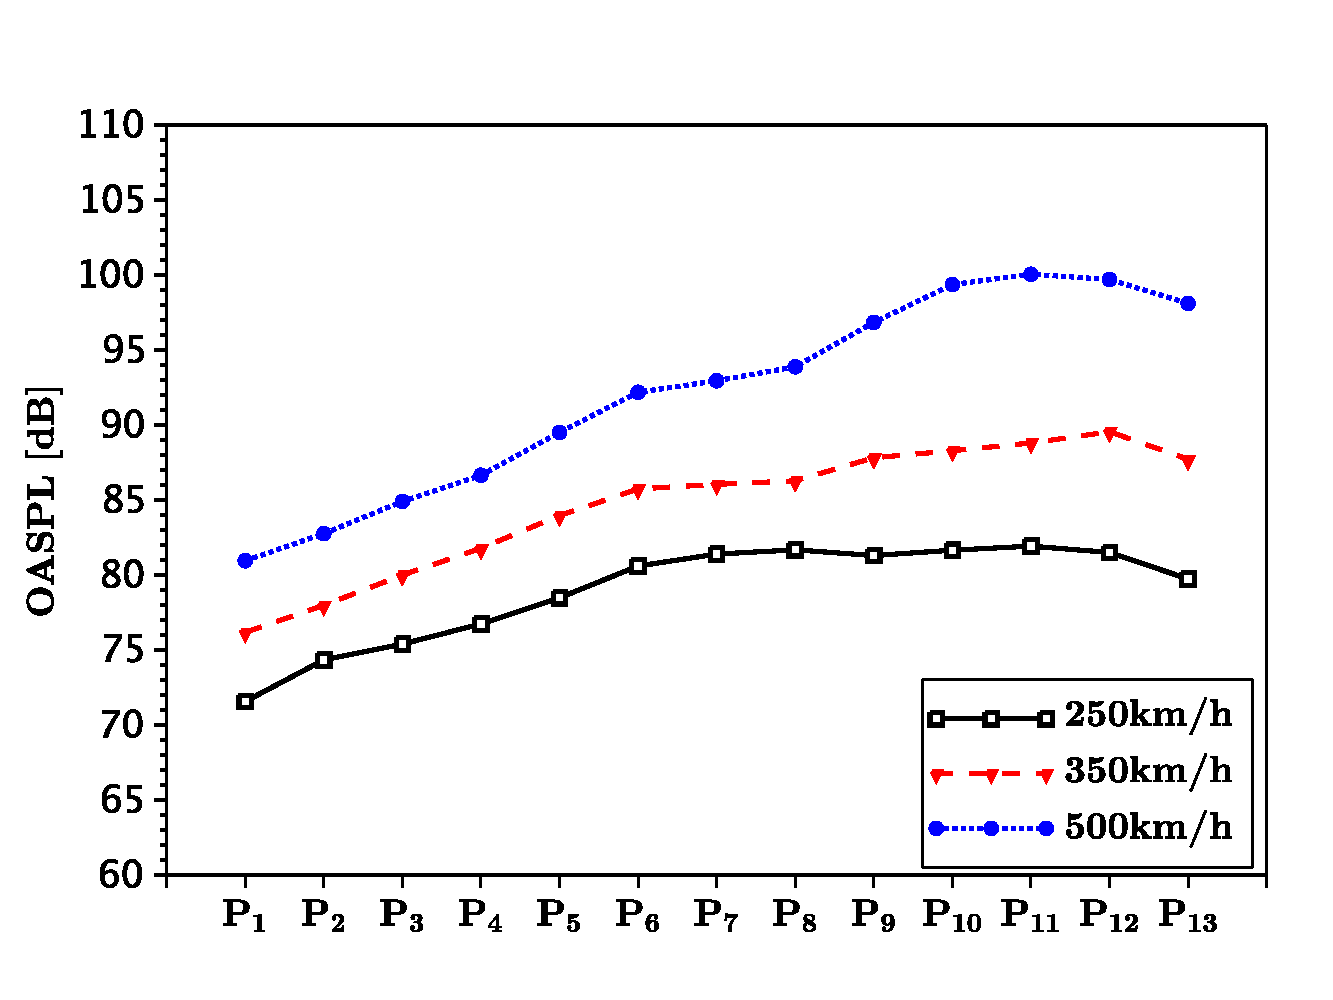
\includegraphics[width=\linewidth]{Figures/oaspl_d.pdf}
    \neusubfigcaption{fig:ch0-four-subfig-d}{工况四}
  \end{neusubfigure}
  \neufigcaption{fig:ch0-four-subfigures}{二乘二子图排版样例}{Example of Two-by-Two Subfigures}
\end{figure}

\neufigref{fig:ch0-four-subfigures} 展示了四幅子图的二乘二排布。
例如 \neusubfigref{fig:ch0-four-subfig-a} 至 \neusubfigref{fig:ch0-four-subfig-d} 可分别引用到四个子图。
排版时建议注意以下几点：
\begin{itemize}
  \item 子图宽度通常可取 \verb|0.48\linewidth| 至 \verb|0.49\linewidth|。
  \item 每行两个子图之间使用 \verb|\hfill| 自动拉开横向间距。
  \item 两行之间可用少量 \verb|\par\vspace| 控制垂直间距。
\end{itemize}

\section{表格排版}

本模板提供 \verb|\neutabcaption{label}{中文题名}{English title}| 用于生成中英文表题。
表题应置于表格上方，正文中使用 \verb|\neutabref{label}| 引用。
表格同样建议使用 \verb|[!htbp]|。如果表格过高导致页底空白，优先考虑缩小字号、调整列宽、拆分表格或使用跨页表格，而不是强制分页。

\subsection{三线表}

\begin{table}[!htbp]
  \centering
  \neutabcaption{tab:ch0-booktabs}{三线表样例}{Example of a Three-Line Table}
  \begin{tabular}{lccc}
    \toprule
    方法       & 准确率（\%）       & 召回率（\%）       & F1 值           \\
    \midrule
    Baseline & 85.2          & 84.1          & 0.846          \\
    Method A & 89.7          & 88.9          & 0.893          \\
    Proposed & \textbf{92.1} & \textbf{91.5} & \textbf{0.918} \\
    \bottomrule
  \end{tabular}
\end{table}

\neutabref{tab:ch0-booktabs} 展示了推荐的三线表格式。
论文中应尽量避免过多竖线，以保持表格简洁。

\subsection{复杂表格}
\begin{table}[!htbp]
  \centering
  \neutabcaption{tab:ch0-complex}{合并单元格与自动换行表格样例}{Example of Merged Cells and Auto-Wrapping Columns}
  \begin{tabularx}{\textwidth}{llXc}
    \toprule
    类别                  & 指标  & 说明                               & 是否必需 \\
    \midrule
    \multirow{2}{*}{图形} & 分辨率 & 位图图片应保证在最终 PDF 中清晰可辨。            & 是    \\
                        & 题名  & 图题使用中英文双语标题，并位于图片下方。             & 是    \\
    \midrule
    \multirow{2}{*}{表格} & 宽度  & 宽表格可使用 \texttt{tabularx} 自动分配列宽。 & 否    \\
                        & 表注  & 表内说明应简明，必要时可在正文中解释。              & 否    \\
    \bottomrule
  \end{tabularx}
\end{table}

\neutabref{tab:ch0-complex} 同时展示了 \verb|\multirow|、\verb|\makecell| 可配合使用的复杂表格场景。
若单元格内容较长，优先使用 \texttt{tabularx} 或 \texttt{p\{...\}} 列类型控制宽度。

\section{公式排版}

公式应使用标准数学环境，并通过 \verb|\label| 设置标签。
引用公式时建议使用模板提供的 \verb|\neueqref{label}|。

\subsection{单行公式}
以分类任务中的交叉熵损失为例，可写为
\begin{equation}
  \mathcal{L}(\theta)
  = - \frac{1}{N}\sum_{i=1}^{N}\sum_{k=1}^{K} y_{ik}\log p_{ik}
  \label{eq:ch0-loss}
\end{equation}

如 \neueqref{eq:ch0-loss} 所示，带编号公式适合放置正文中需要引用的重要定义。

\subsection{多行公式}
循环模型中的状态更新和输出计算可写为
\begin{align}
  h_t       & = \sigma(W_x x_t + W_h h_{t-1} + b), \label{eq:ch0-state} \\
  \hat{y}_t & = \operatorname{softmax}(W_o h_t). \label{eq:ch0-output}
\end{align}

\neueqref{eq:ch0-state} 和 \neueqref{eq:ch0-output} 展示了多行公式的编号方式。
如果多行推导只需要一个编号，可使用 \texttt{aligned} 放在 \texttt{equation} 环境内部。

\subsection{分段函数与矩阵}
分段函数和矩阵经常同时出现在数学定义中，例如
\begin{equation}
  g(x)=
  \begin{cases}
    0, & x < 0,       \\
    x, & 0 \le x < 1, \\
    1, & x \ge 1,
  \end{cases}
  \qquad
  A =
  \begin{bmatrix}
    1 & 0 & 0 \\
    0 & 1 & 0 \\
    0 & 0 & 1
  \end{bmatrix}.
  \label{eq:ch0-piecewise}
\end{equation}

\neueqref{eq:ch0-piecewise} 展示了分段函数和矩阵的常见写法。

\section{算法伪代码}

计算机类论文常需要给出算法步骤。本文档在 \texttt{main.tex} 中加载了 \texttt{algorithm} 和 \texttt{algorithmic} 宏包，可以直接使用如下环境。

\begin{algorithm}[!htbp]
  \caption{样例训练流程}
  \label{alg:ch0-training}
  \begin{algorithmic}[1]
    \REQUIRE Training set $\mathcal{D}$, learning rate $\eta$, maximum epoch $T$
    \ENSURE Model parameters $\theta$
    \STATE Initialize parameters $\theta$
    \FOR{$t = 1$ to $T$}
    \STATE Sample a mini-batch $\mathcal{B}$ from $\mathcal{D}$
    \STATE Compute loss $\mathcal{L}(\theta)$ by \neueqref{eq:ch0-loss}
    \STATE Update $\theta \leftarrow \theta - \eta \nabla_{\theta}\mathcal{L}(\theta)$
    \ENDFOR
    \RETURN $\theta$
  \end{algorithmic}
\end{algorithm}

算法~\ref{alg:ch0-training} 展示了带行号的伪代码。
若需要中文关键字，可在导言区重定义相应命令。

\section{引用、链接与交叉引用}

参考文献引用可使用两种模板命令：
\begin{itemize}
  \item 上标引用使用 \verb|\upcite{key}|，适合放在句末，例如已有研究讨论了神经网络轻量化问题\upcite{guo_2023_research}。
  \item 正文引用使用 \verb|\inlinecite{key}|，适合作为句子成分，例如文献 \inlinecite{thakkar_2018_performance} 给出了系统性能评测案例。
\end{itemize}
多篇文献可写在同一条引用命令中，例如区块链平台相关研究\upcite{zheng_2019_nutbaas,thakkar_2018_performance}。

交叉引用建议统一使用模板命令：
\begin{itemize}
  \item 图引用：\verb|\neufigref{fig:ch0-pdf}|，效果为 \neufigref{fig:ch0-pdf}。
  \item 子图引用：\verb|\neusubfigref{fig:ch0-four-subfig-a}|，效果为 \neusubfigref{fig:ch0-four-subfig-a}。
  \item 表引用：\verb|\neutabref{tab:ch0-complex}|，效果为 \neutabref{tab:ch0-complex}。
  \item 公式引用：\verb|\neueqref{eq:ch0-loss}|，效果为 \neueqref{eq:ch0-loss}。
  \item 算法引用：当前模板未单独封装算法引用命令，可写作“算法~\ref{alg:ch0-training}”。
\end{itemize}
模板提供的公开命令和环境可参考 \texttt{README.md} 中的“模板命令说明”一节。
|。
脚注示例如此处所示\footnote{脚注用于补充说明，不宜放置过长的正文内容。}。
若某页因图表浮动或分页规则没有排满，脚注可能跟随正文排版区而显得略高，这是正常的 LaTeX 页面构建结果。

\subsection{字体、字号与强调}

模板预定义了常用中文字体命令。正式论文中通常不需要手动切换字体；只有在展示样式、术语强调或特殊说明时才建议使用。
当前模板已经为默认宋体和 \verb|\song| 字族配置伪粗体，因此 \verb|\textbf| 或 \verb|\bfseries| 可以用于中文局部强调。
需要注意的是，中文加粗应克制使用；标题层级、术语定义或表格重点值可以适当加粗，大段正文不建议整体加粗。
如果需要更明显的标题式强调，可使用黑体或调整标题层级；如果只是普通正文重点，优先使用 \verb|\textbf|。

\begin{table}[!htbp]
  \centering
  \neutabcaption{tab:ch0-fonts}{字体与强调样例}{Examples of Fonts and Emphasis}
  \begin{tabular}{lll}
    \toprule
    命令             & 显示效果                         & 使用建议       \\
    \midrule
    \verb|\song|   & {\song 宋体文字示例}               & 正文默认字体     \\
    \verb|\textbf| & \textbf{加粗文字示例}              & 局部强调、表格重点值 \\
    \verb|\hei|    & {\hei 黑体文字示例}                & 标题或较强强调场景  \\
    \verb|\kai|    & {\kai 楷体文字示例}                & 摘要、题签或引用语  \\
    \verb|\fs|     & {\fs 仿宋文字示例}                 & 特殊文书类内容    \\
    \verb|\textit| & \textit{Italic text example} & 英文斜体或变量说明  \\
    \bottomrule
  \end{tabular}
\end{table}

\subsection{列表环境}

无序列表适合列出并列事项：
\begin{itemize}
  \item 图题位于图下方，表题位于表上方。
  \item 图表应使用中英文双语标题。
  \item 公式、图、表、算法均应使用标签进行交叉引用。
\end{itemize}

有序列表适合描述步骤：
\begin{enumerate}
  \item 在 \texttt{main.tex} 中填写论文元信息。
  \item 在各章文件中撰写正文内容。
  \item 使用 \texttt{latexmk -xelatex main.tex} 完成编译。
\end{enumerate}

\section{图形排版}

本模板提供 \verb|\neufigcaption{label}{中文题名}{English title}| 用于生成中英文图题。
图题应置于图形下方，正文中使用 \verb|\neufigref{label}| 引用。
图形建议使用 \verb|[!htbp]| 浮动参数，让 LaTeX 在当前位置、页顶、页底或浮动页中选择较合适的位置；除非必须固定位置，否则不建议使用 \verb|[H]|。

\subsection{外部图片}
\begin{figure}[!htbp]
  \centering
  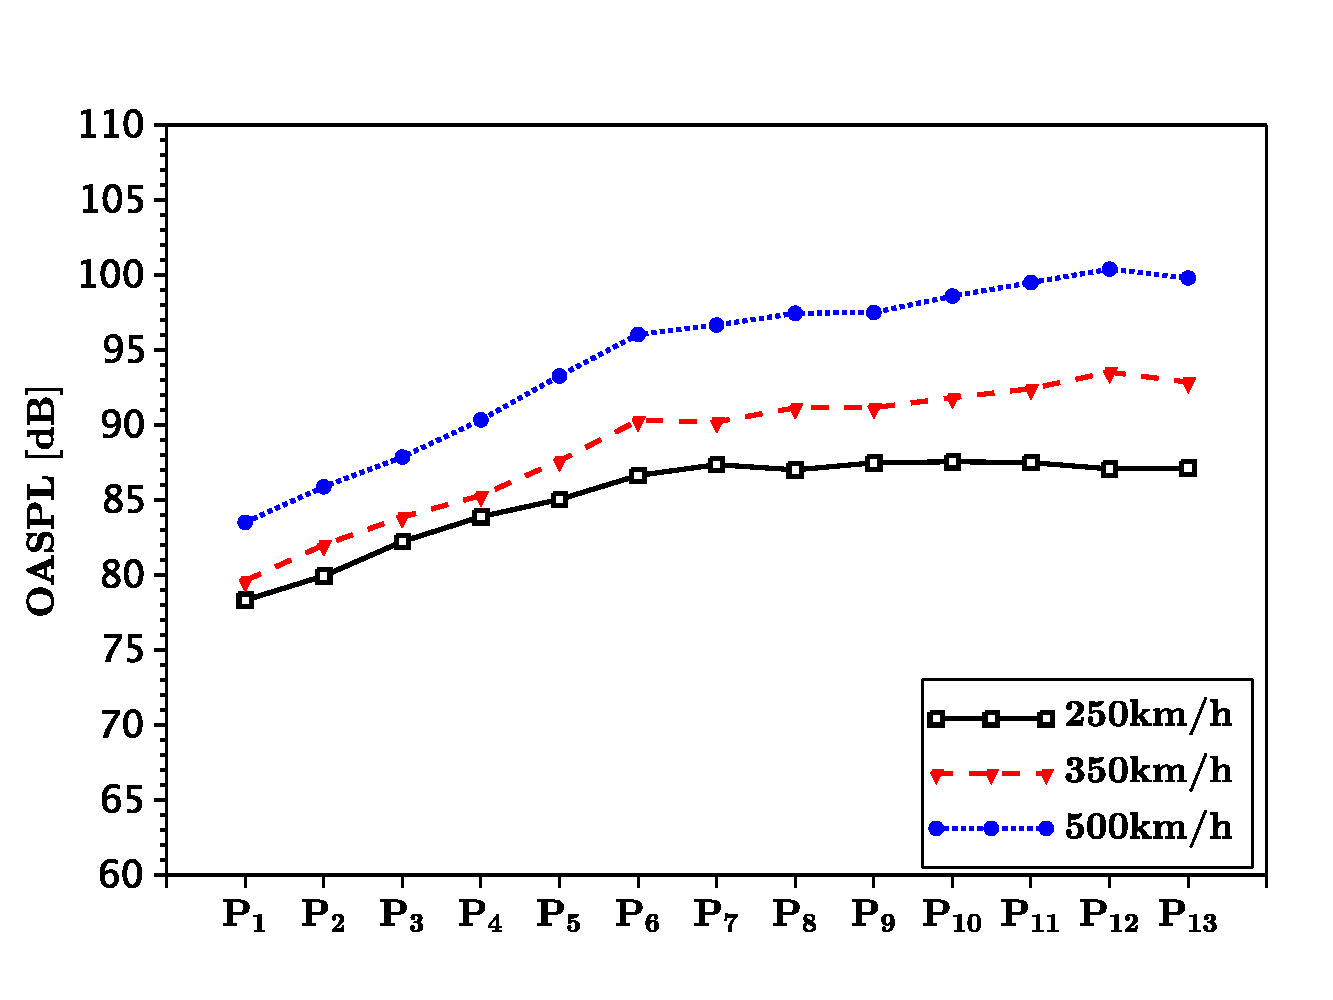
\includegraphics[width=0.55\textwidth]{Figures/oaspl_a.pdf}
  \neufigcaption{fig:ch0-cover}{外部图片插入样例}{Example of Including an External Image}
\end{figure}

\neufigref{fig:ch0-cover} 展示了通过 \verb|\includegraphics| 插入图片文件的方式。
正式论文中建议将图片统一放入 \texttt{Figures} 目录，并使用相对路径引用。

\subsection{PDF 或位图图片}
\begin{figure}[!htbp]
  \centering
  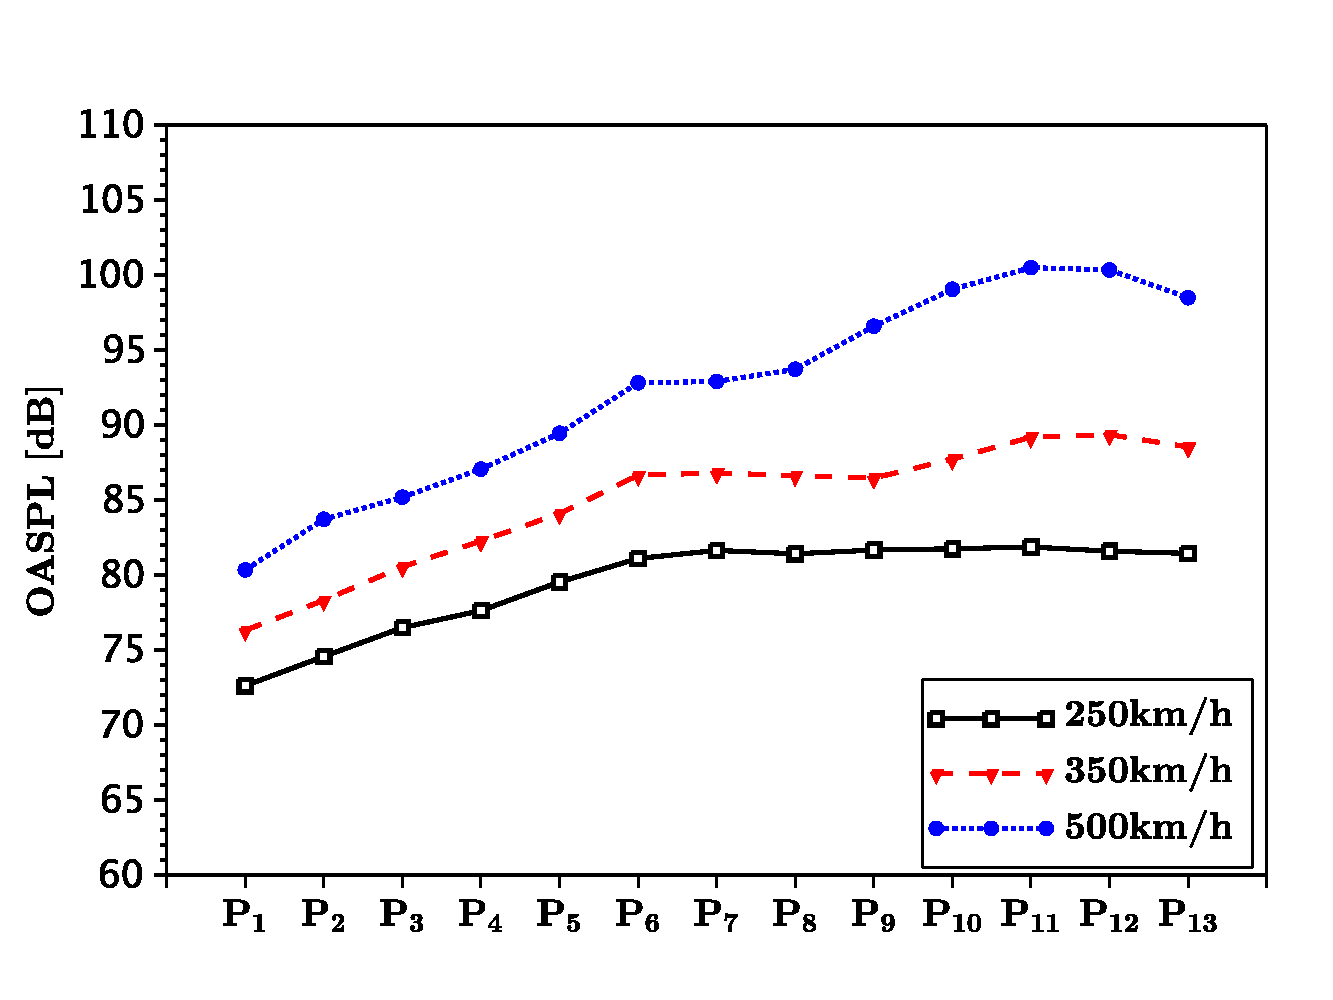
\includegraphics[width=0.55\textwidth]{Figures/oaspl_b.pdf}
  \neufigcaption{fig:ch0-pdf}{PDF 图片插入样例}{Example of Including a PDF Figure}
\end{figure}

PDF、PNG、JPG 等常见图片格式均可通过 \verb|\includegraphics| 插入。
若图片由绘图软件或数据分析程序导出，建议优先使用 PDF 格式以保持较清晰的显示效果。

\subsection{并列图片}
\begin{figure}[!htbp]
  \centering
  \begin{minipage}[t]{0.49\linewidth}
    \centering
    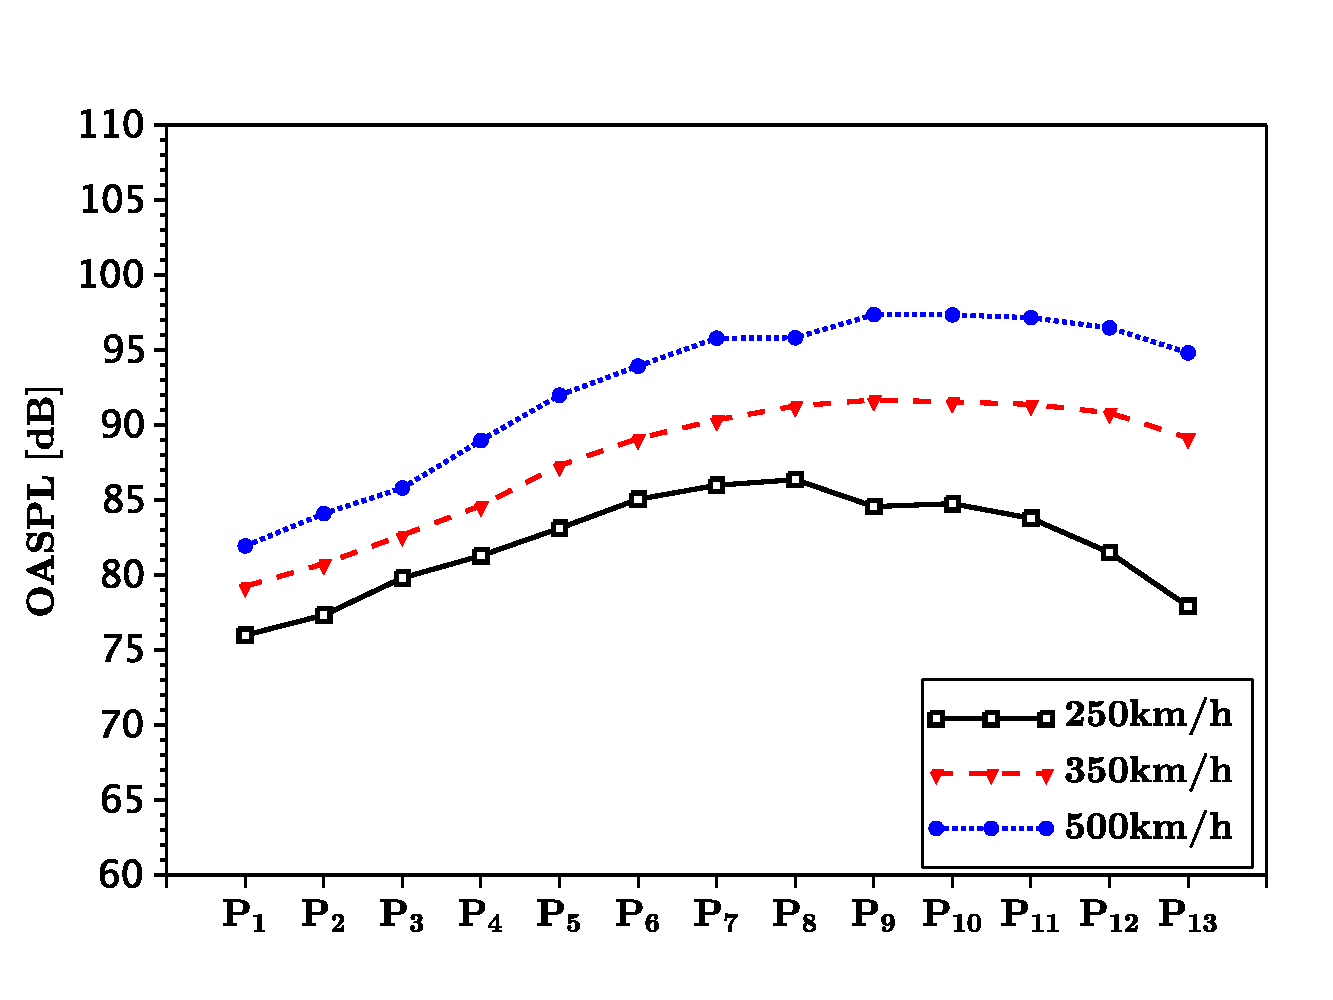
\includegraphics[width=\linewidth]{Figures/oaspl_c.pdf}
  \end{minipage}
  \hfill
  \begin{minipage}[t]{0.49\linewidth}
    \centering
    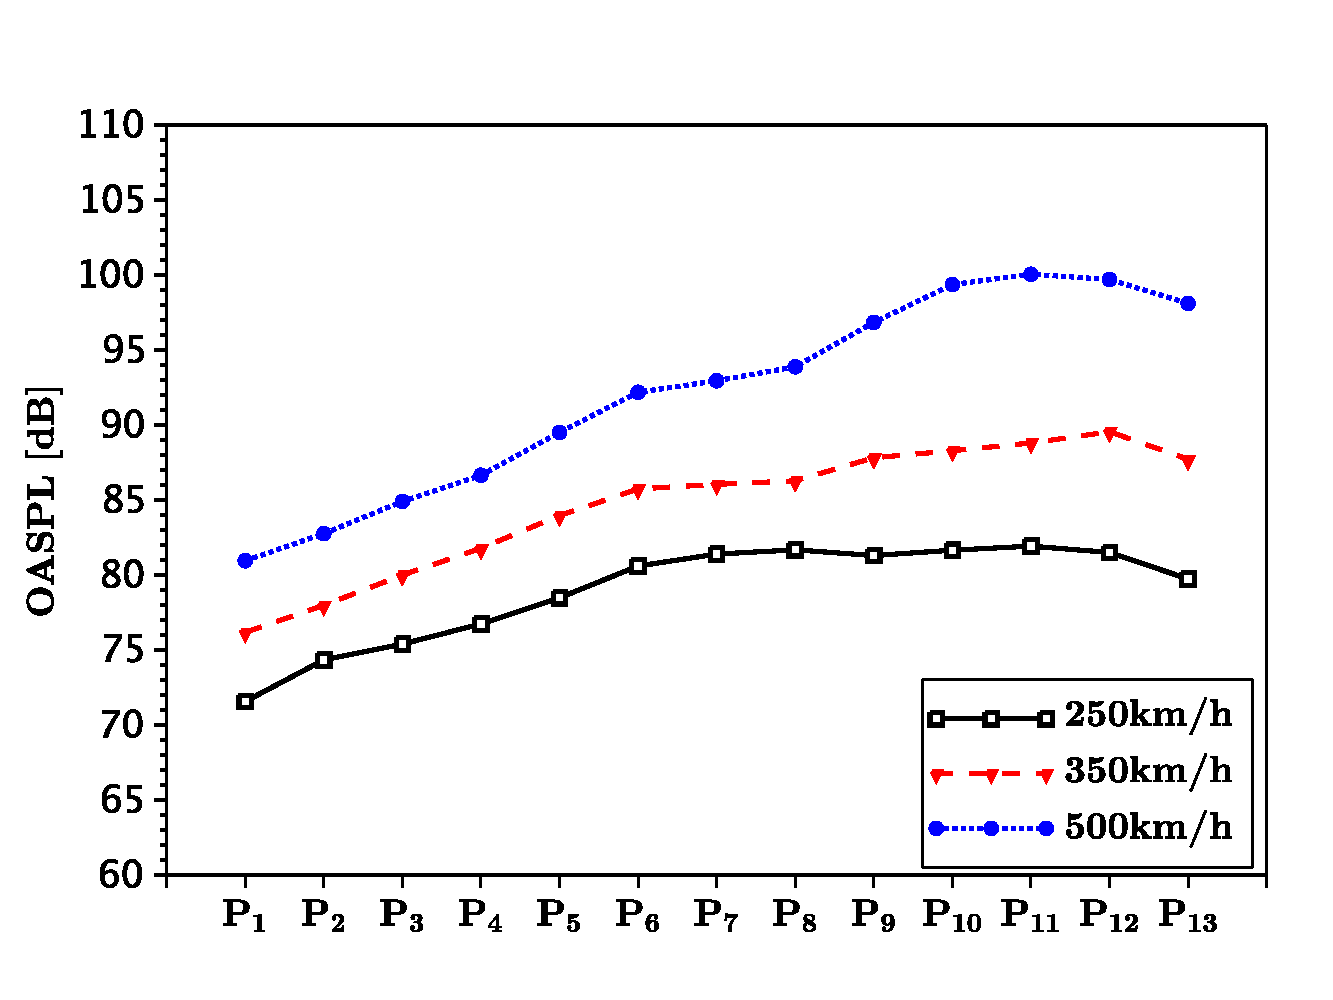
\includegraphics[width=\linewidth]{Figures/oaspl_d.pdf}
  \end{minipage}
  \neufigcaption{fig:ch0-side-by-side}{普通并列图形排版样例}{Example of Side-by-Side Figures}
\end{figure}

\neufigref{fig:ch0-side-by-side} 使用 \texttt{minipage} 完成普通并列排版。
当两幅图共享一个总标题且不需要分别引用时，可使用这种方式。

\subsection{并列子图}
\begin{figure}[!htbp]
  \centering
  \begin{neusubfigure}{0.49\linewidth}
    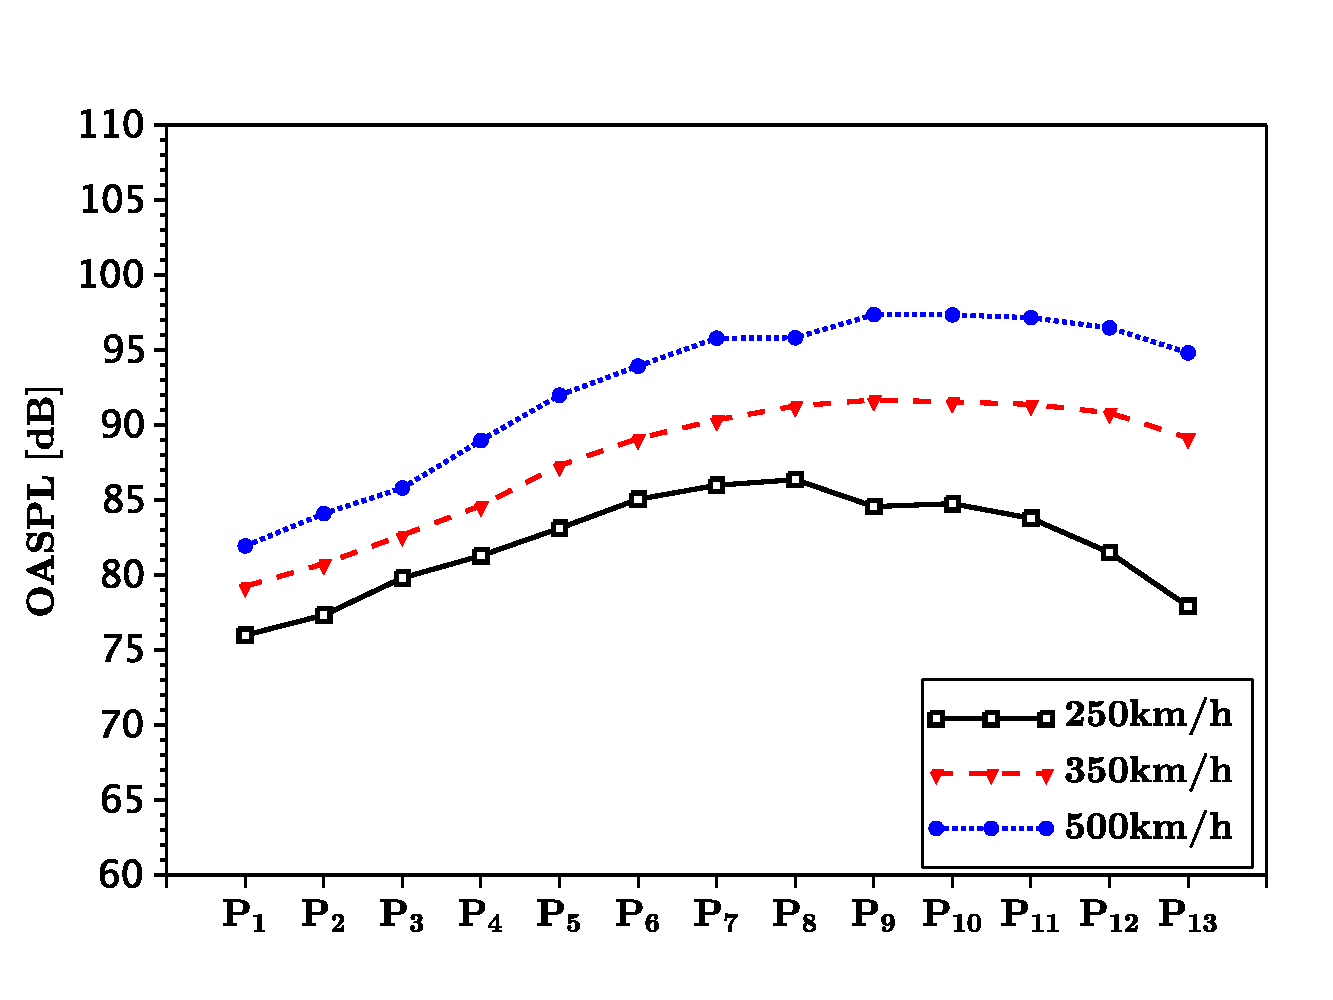
\includegraphics[width=\linewidth]{Figures/oaspl_c.pdf}
    \neusubfigcaption{fig:ch0-side-by-side-a}{工况一}
  \end{neusubfigure}
  \hfill
  \begin{neusubfigure}{0.49\linewidth}
    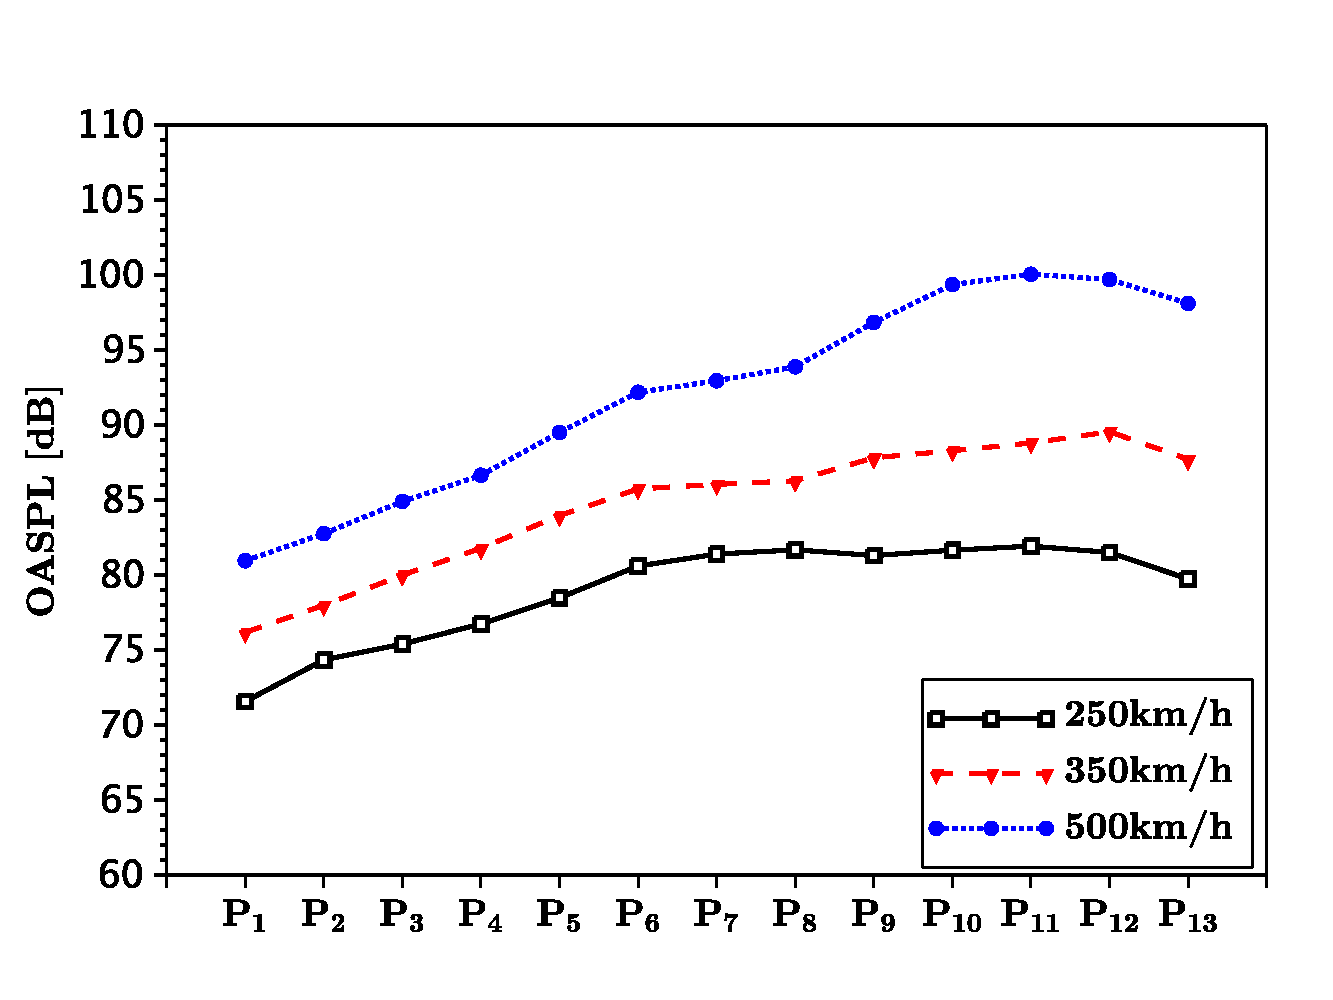
\includegraphics[width=\linewidth]{Figures/oaspl_d.pdf}
    \neusubfigcaption{fig:ch0-side-by-side-b}{工况二}
  \end{neusubfigure}
  \neufigcaption{fig:ch0-subfigures}{并列子图排版样例}{Example of Side-by-Side Subfigures}
\end{figure}

\neufigref{fig:ch0-subfigures} 使用 \texttt{neusubfigure} 完成并列子图排版。
其中 \neusubfigref{fig:ch0-side-by-side-a} 和 \neusubfigref{fig:ch0-side-by-side-b} 可分别引用到子图。
当两幅图共享一个总标题且需要分别引用时，可使用这种方式；如果每幅图需要完全独立的图号，建议拆成两个独立的 \texttt{figure} 环境。

\subsection{二乘二子图}
\begin{figure}[!htbp]
  \centering
  \begin{neusubfigure}{0.49\linewidth}
    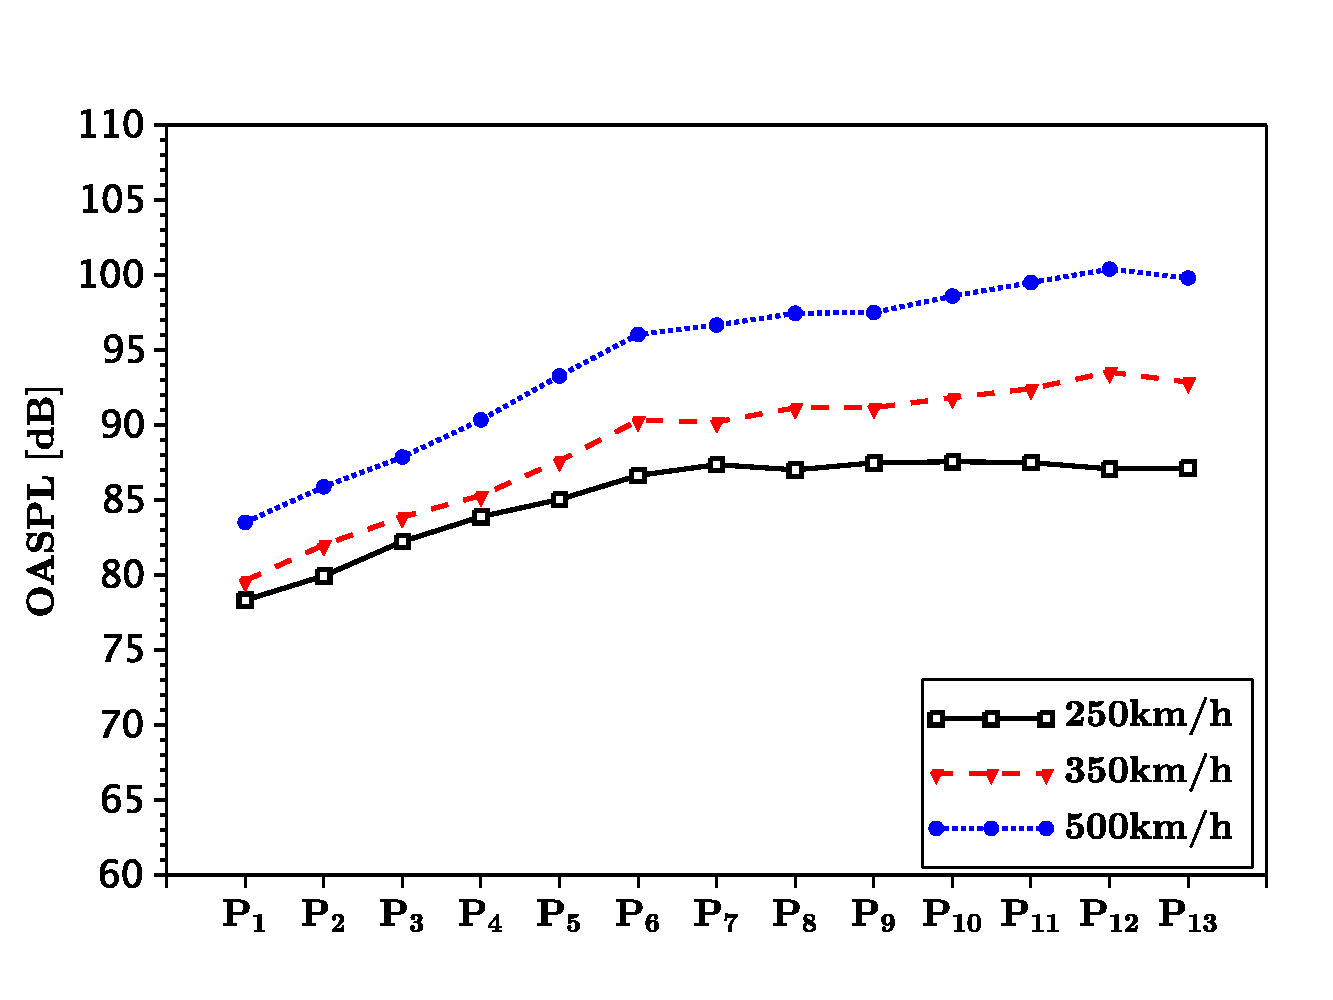
\includegraphics[width=\linewidth]{Figures/oaspl_a.pdf}
    \neusubfigcaption{fig:ch0-four-subfig-a}{工况一}
  \end{neusubfigure}
  \hfill
  \begin{neusubfigure}{0.49\linewidth}
    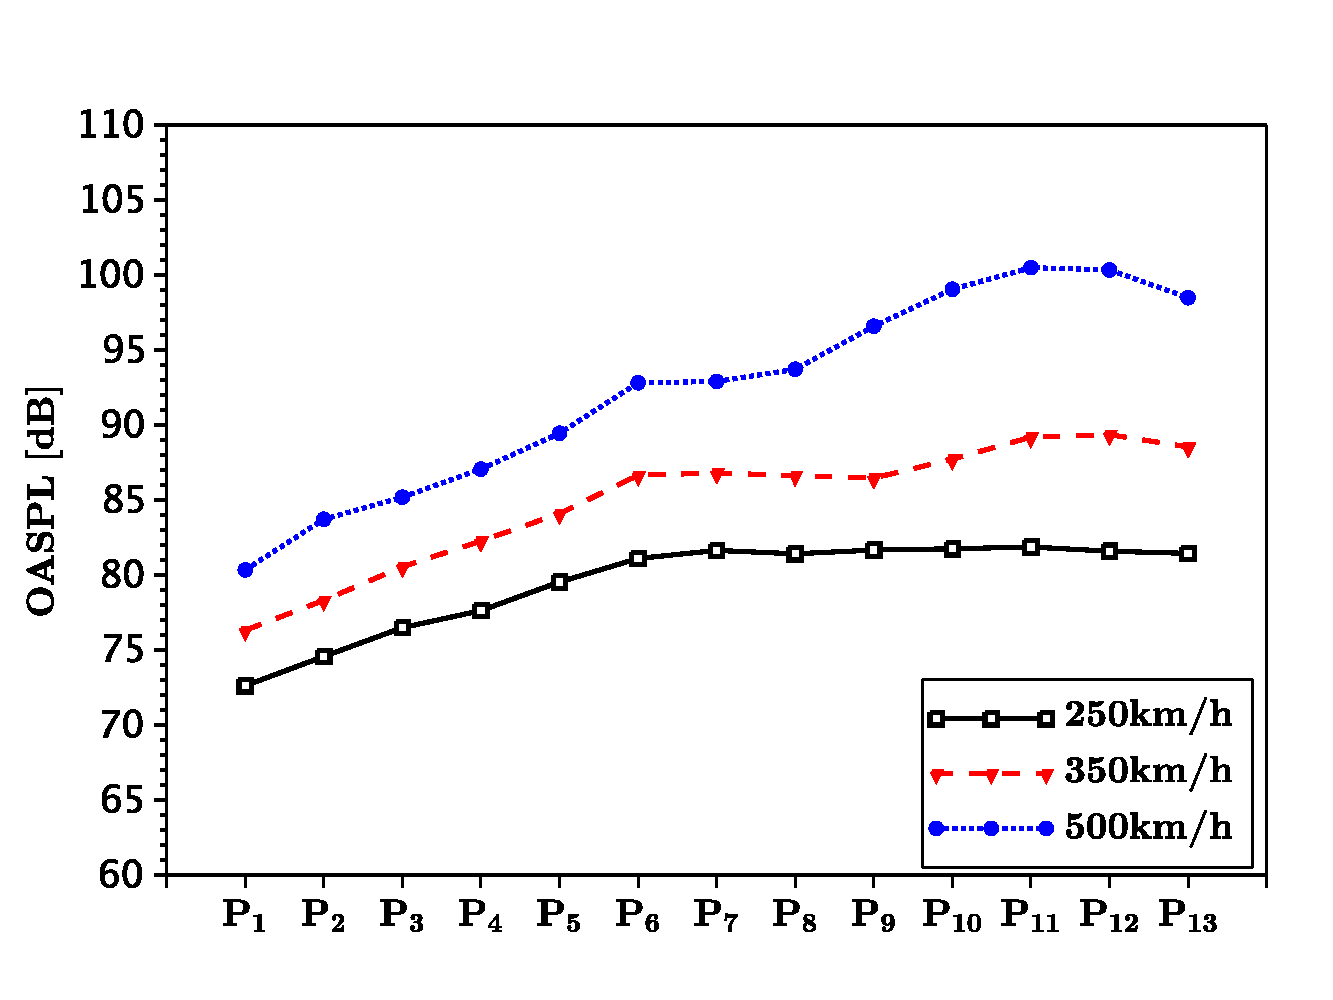
\includegraphics[width=\linewidth]{Figures/oaspl_b.pdf}
    \neusubfigcaption{fig:ch0-four-subfig-b}{工况二}
  \end{neusubfigure}
  \par\vspace{2bp}

  \begin{neusubfigure}{0.49\linewidth}
    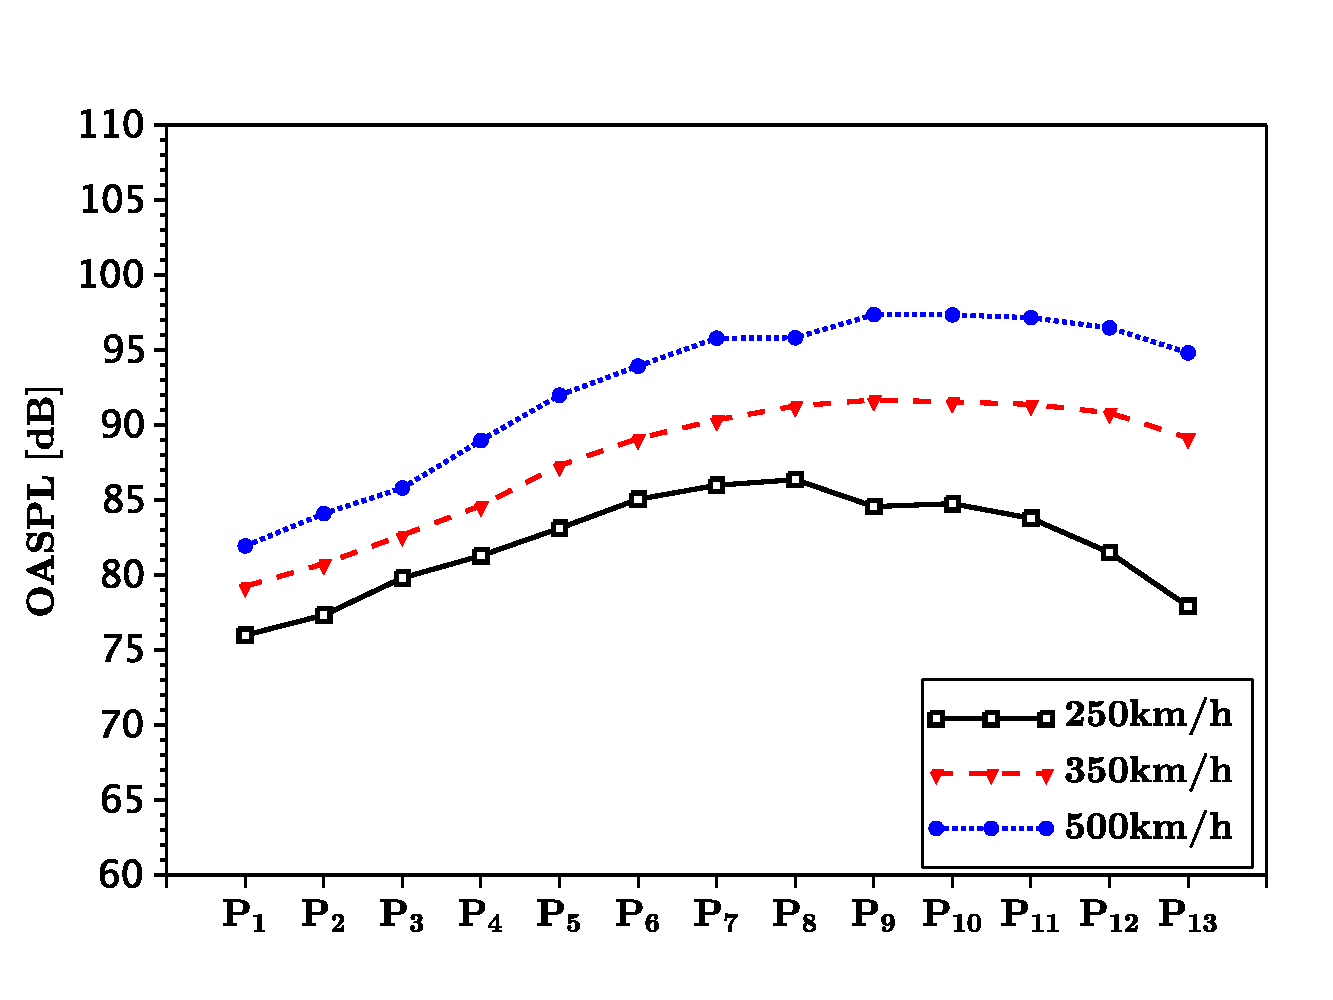
\includegraphics[width=\linewidth]{Figures/oaspl_c.pdf}
    \neusubfigcaption{fig:ch0-four-subfig-c}{工况三}
  \end{neusubfigure}
  \hfill
  \begin{neusubfigure}{0.49\linewidth}
    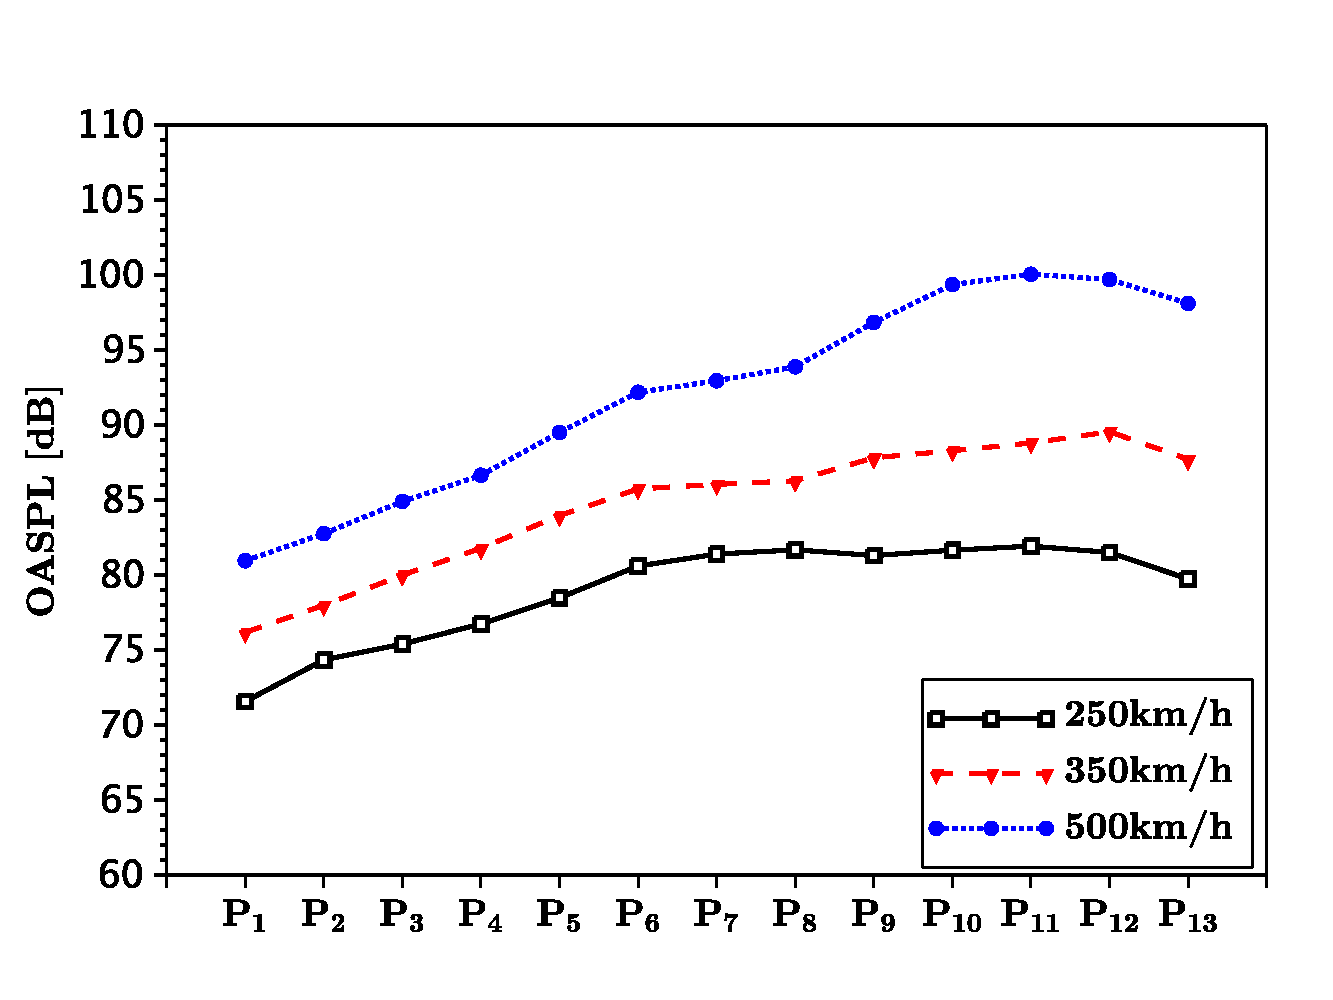
\includegraphics[width=\linewidth]{Figures/oaspl_d.pdf}
    \neusubfigcaption{fig:ch0-four-subfig-d}{工况四}
  \end{neusubfigure}
  \neufigcaption{fig:ch0-four-subfigures}{二乘二子图排版样例}{Example of Two-by-Two Subfigures}
\end{figure}

\neufigref{fig:ch0-four-subfigures} 展示了四幅子图的二乘二排布。
例如 \neusubfigref{fig:ch0-four-subfig-a} 至 \neusubfigref{fig:ch0-four-subfig-d} 可分别引用到四个子图。
排版时建议注意以下几点：
\begin{itemize}
  \item 子图宽度通常可取 \verb|0.48\linewidth| 至 \verb|0.49\linewidth|。
  \item 每行两个子图之间使用 \verb|\hfill| 自动拉开横向间距。
  \item 两行之间可用少量 \verb|\par\vspace| 控制垂直间距。
\end{itemize}

\section{表格排版}

本模板提供 \verb|\neutabcaption{label}{中文题名}{English title}| 用于生成中英文表题。
表题应置于表格上方，正文中使用 \verb|\neutabref{label}| 引用。
表格同样建议使用 \verb|[!htbp]|。如果表格过高导致页底空白，优先考虑缩小字号、调整列宽、拆分表格或使用跨页表格，而不是强制分页。

\subsection{三线表}

\begin{table}[!htbp]
  \centering
  \neutabcaption{tab:ch0-booktabs}{三线表样例}{Example of a Three-Line Table}
  \begin{tabular}{lccc}
    \toprule
    方法       & 准确率（\%）       & 召回率（\%）       & F1 值           \\
    \midrule
    Baseline & 85.2          & 84.1          & 0.846          \\
    Method A & 89.7          & 88.9          & 0.893          \\
    Proposed & \textbf{92.1} & \textbf{91.5} & \textbf{0.918} \\
    \bottomrule
  \end{tabular}
\end{table}

\neutabref{tab:ch0-booktabs} 展示了推荐的三线表格式。
论文中应尽量避免过多竖线，以保持表格简洁。

\subsection{复杂表格}
\begin{table}[!htbp]
  \centering
  \neutabcaption{tab:ch0-complex}{合并单元格与自动换行表格样例}{Example of Merged Cells and Auto-Wrapping Columns}
  \begin{tabularx}{\textwidth}{llXc}
    \toprule
    类别                  & 指标  & 说明                               & 是否必需 \\
    \midrule
    \multirow{2}{*}{图形} & 分辨率 & 位图图片应保证在最终 PDF 中清晰可辨。            & 是    \\
                        & 题名  & 图题使用中英文双语标题，并位于图片下方。             & 是    \\
    \midrule
    \multirow{2}{*}{表格} & 宽度  & 宽表格可使用 \texttt{tabularx} 自动分配列宽。 & 否    \\
                        & 表注  & 表内说明应简明，必要时可在正文中解释。              & 否    \\
    \bottomrule
  \end{tabularx}
\end{table}

\neutabref{tab:ch0-complex} 同时展示了 \verb|\multirow|、\verb|\makecell| 可配合使用的复杂表格场景。
若单元格内容较长，优先使用 \texttt{tabularx} 或 \texttt{p\{...\}} 列类型控制宽度。

\section{公式排版}

公式应使用标准数学环境，并通过 \verb|\label| 设置标签。
引用公式时建议使用模板提供的 \verb|\neueqref{label}|。

\subsection{单行公式}
以分类任务中的交叉熵损失为例，可写为
\begin{equation}
  \mathcal{L}(\theta)
  = - \frac{1}{N}\sum_{i=1}^{N}\sum_{k=1}^{K} y_{ik}\log p_{ik}
  \label{eq:ch0-loss}
\end{equation}

如 \neueqref{eq:ch0-loss} 所示，带编号公式适合放置正文中需要引用的重要定义。

\subsection{多行公式}
循环模型中的状态更新和输出计算可写为
\begin{align}
  h_t       & = \sigma(W_x x_t + W_h h_{t-1} + b), \label{eq:ch0-state} \\
  \hat{y}_t & = \operatorname{softmax}(W_o h_t). \label{eq:ch0-output}
\end{align}

\neueqref{eq:ch0-state} 和 \neueqref{eq:ch0-output} 展示了多行公式的编号方式。
如果多行推导只需要一个编号，可使用 \texttt{aligned} 放在 \texttt{equation} 环境内部。

\subsection{分段函数与矩阵}
分段函数和矩阵经常同时出现在数学定义中，例如
\begin{equation}
  g(x)=
  \begin{cases}
    0, & x < 0,       \\
    x, & 0 \le x < 1, \\
    1, & x \ge 1,
  \end{cases}
  \qquad
  A =
  \begin{bmatrix}
    1 & 0 & 0 \\
    0 & 1 & 0 \\
    0 & 0 & 1
  \end{bmatrix}.
  \label{eq:ch0-piecewise}
\end{equation}

\neueqref{eq:ch0-piecewise} 展示了分段函数和矩阵的常见写法。

\section{算法伪代码}

计算机类论文常需要给出算法步骤。本文档在 \texttt{main.tex} 中加载了 \texttt{algorithm} 和 \texttt{algorithmic} 宏包，可以直接使用如下环境。

\begin{algorithm}[!htbp]
  \caption{样例训练流程}
  \label{alg:ch0-training}
  \begin{algorithmic}[1]
    \REQUIRE Training set $\mathcal{D}$, learning rate $\eta$, maximum epoch $T$
    \ENSURE Model parameters $\theta$
    \STATE Initialize parameters $\theta$
    \FOR{$t = 1$ to $T$}
    \STATE Sample a mini-batch $\mathcal{B}$ from $\mathcal{D}$
    \STATE Compute loss $\mathcal{L}(\theta)$ by \neueqref{eq:ch0-loss}
    \STATE Update $\theta \leftarrow \theta - \eta \nabla_{\theta}\mathcal{L}(\theta)$
    \ENDFOR
    \RETURN $\theta$
  \end{algorithmic}
\end{algorithm}

算法~\ref{alg:ch0-training} 展示了带行号的伪代码。
若需要中文关键字，可在导言区重定义相应命令。

\section{引用、链接与交叉引用}

参考文献引用可使用两种模板命令：
\begin{itemize}
  \item 上标引用使用 \verb|\upcite{key}|，适合放在句末，例如已有研究讨论了神经网络轻量化问题\upcite{guo_2023_research}。
  \item 正文引用使用 \verb|\inlinecite{key}|，适合作为句子成分，例如文献 \inlinecite{thakkar_2018_performance} 给出了系统性能评测案例。
\end{itemize}
多篇文献可写在同一条引用命令中，例如区块链平台相关研究\upcite{zheng_2019_nutbaas,thakkar_2018_performance}。

交叉引用建议统一使用模板命令：
\begin{itemize}
  \item 图引用：\verb|\neufigref{fig:ch0-pdf}|，效果为 \neufigref{fig:ch0-pdf}。
  \item 子图引用：\verb|\neusubfigref{fig:ch0-four-subfig-a}|，效果为 \neusubfigref{fig:ch0-four-subfig-a}。
  \item 表引用：\verb|\neutabref{tab:ch0-complex}|，效果为 \neutabref{tab:ch0-complex}。
  \item 公式引用：\verb|\neueqref{eq:ch0-loss}|，效果为 \neueqref{eq:ch0-loss}。
  \item 算法引用：当前模板未单独封装算法引用命令，可写作“算法~\ref{alg:ch0-training}”。
\end{itemize}
模板提供的公开命令和环境可参考 \texttt{README.md} 中的“模板命令说明”一节。
